%\documentclass[11pt]{proc}
\documentclass[11pt,twocolumn]{article}

\usepackage{graphicx}

\usepackage{subcaption}
\usepackage{epstopdf}
\usepackage{float}
\usepackage{pgfplots}
\usepackage[export]{adjustbox}


\usepackage{hyperref}
\usepackage{cleveref}

\usepackage[round]{natbib}

\usepackage{verbatim}

\usepackage{amsmath}
\usepackage{mathtools}
\usepackage{esint}
\usepackage{mathrsfs}
\usepackage{xfrac}
\usepackage{tabularx}

\usepackage{geometry}

\usepackage[titletoc]{appendix}

\usepackage{subeqnarray}

\usepgfplotslibrary{external} 
\tikzexternalize[prefix=./figures/]

\graphicspath{ {./figures/} }

\renewcommand{\sectionautorefname}{\S}
\renewcommand{\subsectionautorefname}{\S}

\newcommand{\St}{\mathscr{S}}
\newcommand{\CompRatio}{\mathscr{C}}

\newcommand{\crefrangeconjunction}{--}

\newcommand{\squeezeup}{\vspace{-5mm}}
\newcommand{\squeezeupsmall}{\vspace{-2.5mm}}

\usepackage[compact]{titlesec}  
%\titlespacing{\section}{8pt}{10pt}{8pt}

\usepackage[labelformat=simple]{subcaption}
\renewcommand\thesubfigure{(\alph{subfigure})}

\captionsetup[figure]{skip=4pt}

\makeatletter
\newcommand{\specialnumber}[1]{%
  \def\tagform@##1{\maketag@@@{(\ignorespaces##1\unskip\@@italiccorr#1)}}%
}
\newcommand{\specialeqref}[2]{\begingroup
  \def\tagform@##1{\maketag@@@{(\ignorespaces##1\unskip\@@italiccorr#2)}}%
  \eqref{#1}\endgroup}
\makeatother

\addtolength{\topmargin}{-.4in}
\addtolength{\bottommargin}{-.875in}


\begin{document}

\bibliographystyle{plainnat}

%set the line spacing, 13pt is the minimum allowed
\setlength{\baselineskip}{13pt}

%use one column for the title page
\onecolumn

\begin{comment}
%remove the page number from the title page
\clearpage
\thispagestyle{empty}
Candidate number: ... \\
Project number : AO04 \\
Project Title: The seeds of “brinicles”: flow and pattern formation in sea ice and mushy layers \\
The supervisor`s name: Dr A Wells and Dr D Rees-Jones \\
Word count: ...

%start the actual report
%\newpage

\end{comment}

\twocolumn

%set this as page 1
\setcounter{page}{1}

\twocolumn[
  \begin{@twocolumnfalse}
\begin{center}
\huge \textbf{The seeds of `brinicles': flow and pattern formation in sea ice and mushy layers} \normalsize
\end{center}
\squeezeup
\begin{abstract}
During the growth of young sea ice a porous mushy layer forms, consisting of ice crystals bathed in liquid brine, within which convection drives salt fluxes between the ice and the ocean. For a sufficiently large Rayleigh number, channels of liquid brine form within the mushy layer as part of buoyancy-driven convection cells. In contrast to previous studies, which consider a two dimensional planar geometry, I present a model for an axisymmetric cylindrical convection cell which has more physical relevance to sea ice. In doing so I introduce a number of novel simplifying assumptions and methods. In particular, the numerical scheme is implemented on a fixed grid, whilst the free boundary between the brine channel and mushy layer is determined by extrapolation. The behaviour of the system is investigated across a range of Rayleigh numbers and for different sizes of convection cell. In particular, conditions for the presence of brine channels and measures of the magnitude of convection are determined. Comparisons are made with the results of other studies, including a theoretical axisymmetric model and numerical planar models, all of which agree with the observed salt flux parametrizations for large Rayleigh numbers ($50 < Rm < 75$). An instability in the numerical method prevents the resolution of steady states at low Rayleigh numbers ($Rm\sim15$), where differences are expected to occur between flow in the two geometries. It is suggested that implementing a more stable method for determining the size of the brine channel may enable future models to overcome this difficulty.
\end{abstract}
  \end{@twocolumnfalse}
  ]
  
  

\section{Introduction}
\label{sec:intro}
Between 1978 and 2014 the September minimum of Arctic sea ice extent fell by 40.2\%~\citep*{fetterer-02}. Over the same time period, the March maximum extent fell by only 8.7\% and, consequently, a greater area of the Arctic ocean is being refrozen each year. It is therefore of increasing importance that the processes involved in the formation of new sea ice are well understood, such that they can be accurately incorporated into general circulation models. 

In the presence of a cold atmosphere, sea ice forms on the surface of the ocean. This ice is a reactive porous medium consisting of solid ice crystals of low salinity surrounded by an interstitial highly-saline fluid, or brine; such a composite mixture is referred to as a mushy layer. When the mushy layer is cooled the ice crystals grow, reducing the volume occupied by the brine and therefore increasing its salinity. Therefore the salinity is greatest where the temperature is coldest, at the top of the mushy layer, and decreases towards the ocean at the bottom. This gradient drives convection; the super-saline liquid sinks, being replaced by the more buoyant and relatively fresh ocean water. 

A sinking brine parcel has a greater salinity and lower temperature than the local equilibrium. The diffusion of salt is a significantly slower process than the diffusion of heat~\citep*{worster-97}, so local equilibrium is recovered by the melting of ice crystals. The resulting increase in the local liquid volume decreases salinity, whilst the latent heat supplied to melt the solid phase causes cooling. Conversely, rising ocean water is less saline and warmer than its environment and leads to freezing in the mushy layer. Permeability increases as local solid fraction decreases, so is greater where the flow is downward and reduced where the flow is rising. A larger permeability in the downward region permits a stronger flow, which in turn leads to greater melting and eventually the formation of entirely liquid channels, or `chimneys', into which the flow of brine out of the mushy layer is focussed. This process is illustrated in figure~\ref{subfig:convection-in-sea-ice}.

Drainage of brine from sea ice increases the salinity and density of the ocean below. This is known to have an effect on the large scale ocean circulation \citep*{brandon-et-al-10}, whilst the physical properties of the newly formed sea ice are dependant on the quantity of interstitial brine that remains \citep*{petrich-eicken-10}. There are other process through which desalination of sea ice can occur, however a review by \citet*{notz-worster-09} concluded that the only significant process in the winter freezing season (October - March) is buoyancy-driven convection. 

Strong salt fluxes attributed to convection have been observed in the Arctic Ocean \citep*{wettlaufer-et-al-00} and the dense, cold, plumes emanating from them have recently been captured on camera in the Antarctic Ocean~\citep[2011]{frozen-planet-11}. These processes have been reproduced using analogous binary mixtures. For example,~\citet*{wettlaufer-et-al-97} studied NaCl-water solutions cooled from above, whilst several studies have considered $\textrm{NH}_4\textrm{Cl}$-water solutions in which $\textrm{NH}_4\textrm{Cl}$ crystals are formed at the cooled base of a tank. A detailed review of these experiments is presented in~\citet*{zhong-et-al-12}.


\begin{figure*}[t]
\centering
\captionsetup[subfigure]{position=top,singlelinecheck=off,justification=raggedright, aboveskip=-12pt,belowskip=0pt}
\begin{subfigure}[t]{.55\linewidth}
    \centering
    \caption{}
    \includegraphics[width=\linewidth]{convection-in-sea-ice.pdf}
    
    \label{subfig:convection-in-sea-ice}
\end{subfigure}
\quad
\captionsetup[subfigure]{ aboveskip=4pt}
\begin{subfigure}[t]{.36\linewidth}
   \centering
   \caption{}
    \includegraphics[width=0.9\linewidth, right]{mushy-layer-chimneys-photo-schulze-worster.jpg}
    
    \label{subfig:schulze-worster-photo}
\end{subfigure}

\caption{~\subref{subfig:convection-in-sea-ice} Summary of steady state buoyancy-driven convection during the formation of sea ice with fully developed chimneys. Thick arrowed lines are streamlines of fluid flow, which circulate from the underlying ocean through the porous ice and out of the chimneys. The grey circles on the right represent ice crystals, illustrating the reduced permeability at the top of the mushy layer. Temperature, $T$, and salinity, $C$, are both indicated.~\subref{subfig:schulze-worster-photo} Photograph of $\textrm{NH}_4\textrm{Cl}$ directional solidification. Notice the formation of narrow, roughly straight sided, chimneys, and also that, apart from where the chimneys meet the liquid phase, the mush-liquid boundary is roughly flat. Taken from Schulze \& Worster (1998), but reflected in the horizontal plane to conform with the orientation of sea ice.}

\setlength{\belowcaptionskip}{0pt} % make text closer to caption

 \label{fig:overview-diagram-photo}

\end{figure*}


An alternative approach studies convection over a wide range of parameters using numerical models, although solving the full problem in this way is both theoretically and computationally cumbersome. Therefore, motivated by experimental observations and a desire for mathematical tractability, a variety of assumptions and simplifications must be introduced. A brief overview of the existing literature is given below, whilst the methods most relevant to this study are described in greater detail in~\autoref{sec:problem-formulation}.

%whilst more details are provided in~\autoref{sec:problem-formulation} in parallel with a description of the approximations made in this paper.

~\citet*{schulze-worster-98} considered a two-dimensional planar arrangement, in which both the chimney wall and the mush-ocean boundary were modelled as straight sides (figure~\ref{fig:arrangement}). Such an approximation is consistent to first order with experiment, as illustrated in figure~\ref{subfig:schulze-worster-photo}, and is ultimately the same approach that I will take.~\citet*{chung-worster-02} also solved numerically for a viscous flow in the liquid region, allowing them to apply jump conditions across the mush-liquid boundaries and hence resolve their shape. This approach confirmed that a straight sided chimney is a good approximation near the mush-ocean boundary, but less accurate away from ocean where the chimney width can decrease to $0$. Solving for the flow in the liquid region is computationally expensive. Therefore more recent studies \citep*{wells-et-al-10, wells-et-al-13} have combined the Schulze \& Worster approach to the mush-liquid boundary with Chung \& Worster's treatment of the chimney wall. 

All these studies are based on a two dimensional planar model and, as shown by~\citet*{rees-jones-worster-13}, axisymmetric convection displays important qualitative differences. For example, salt flux strongly depends on the far field ocean temperature in axisymmetry but does not in a planar geometry. Moreover,~\citet*{rees-jones-worster-13} also demonstrated that full three dimensional convection could be reasonably approximated by an axisymmetric arrangement. Their results were obtained by constructing a simple model which, through a similarity solution, reduced to a system of ordinary differential equations. In order to test the robustness of their conclusions, I construct a full numerical model for convective flow through brine channels in an axisymmetric geometry. For simplicity, I apply Schulze \& Worster's assumptions of a straight sided chimney and flat mush-ocean boundary and focus on solutions with no azimuthal variation.

The derivation of the governing equations and boundary conditions is presented in~\autoref{sec:problem-formulation}. In~\autoref{sec:computational-procedure} I describe the numerical methods used to solve the problem and how the solution has been verified. Steady states are then found for a range of parameters, and the results of these simulations are presented and discussed in~\autoref{sec:results}. Finally, I conclude in~\autoref{sec:conclusion}.

\section{Problem formulation}
\label{sec:problem-formulation}

\begin{figure*}[t]
       \centering
        \includegraphics[width=\textwidth]{simplified-arrangement}
        \setlength{\belowcaptionskip}{0pt} % make text closer to caption
        
       \caption{Simplified mushy layer geometry (left) showing a radial cross section of an axisymmetric annular region. Dashed lines show the geometry of the full non-linear problem, for comparison. At the top of the convection cell, the mushy layer is at the eutectic temperature - the point where, for any liquid concentration, the binary mixture forms an impermeable solid. This can be seen in the phase diagram (right) where the thick black line illustrates the path taken by a fluid parcel as it is cooled from the ocean to the eutectic solid, under the assumption that it is always in thermodynamic equilibrium.}
    \label{fig:arrangement}
\end{figure*}

I consider steady state convection in a cylindrical region of a mushy layer with a chimney at the centre, as shown in figure~\ref{fig:arrangement}. The chimney is centred on $r=0$ and has radius $a$, whilst the full convection cell has radius $R$ and height $H$. At the top of the mushy layer is a region of ice at or below the eutectic temperature, $T_E$, which is defined as the point at which the binary mixture becomes impermeable for all values of the solute concentration $C$. In line with the previous studies mentioned in~\autoref{sec:intro}, this region is assumed to grow downwards at a constant rate $V$. Although this is not truly representative of sea ice, where the growth rate decreases as freezing progresses, it is a simplifying assumption that allows for steady state solutions. The reference frame is chosen so that the origin remains fixed at the base of the eutectic solid. From this perspective, the mushy layer is pulled upwards between two fixed heat exchangers at the growth rate, $V$.

Following previous authors, I assume that the mushy layer is ideal \citep*{worster-97}. Within this assumption, the temperature $T$ and solute concentration, or salinity, $C$ are in local thermodynamic equilibrium and obey a linear liquidus relationship

\begin{equation}
\label{eq:liquidus}
T = T_L(C) = T_E  - \Gamma (C-C_E) \;
\end{equation}
where $\Gamma$ is the slope of the liquidus. The ocean is assumed to have constant salinity $C_0$ and the temperature at the mush-liquid boundary is therefore given by $T_0 = T_L(C_0)$. The far field temperature in the ocean is $T_\infty$.

\subsection{Governing equations}
Flow in an ideal mushy layer is governed by Darcy's equation for flow in a porous medium, and is assumed to be incompressible:
%\begin{equation}
%\label{eq:darcys-eqn}
 %\mathbf{u} = \frac{\Pi}{\mu} (- \nabla p + \rho \mathbf{g}); \hspace{15ex} \nabla \cdot \mathbf{u} = 0,
%\end{equation}

%\newcolumntype{R}{>{\raggedleft\arraybackslash}X}
  \begin{equation}
  \specialnumber{a,b} \label{eq:darcys-eqn-incompressible} 
  \mathbf{u} = \frac{\Pi}{\mu} (- \nabla p + \rho \mathbf{g}),  \qquad  \nabla \cdot \mathbf{u} = 0,
  \end{equation}
where $\mathbf{u}$ represents the flux of the interstitial fluid relative to the solid phase, known as the Darcy velocity. I have also introduced the permeability $\Pi$, pressure $p$, dynamic viscosity $\mu$, density $\rho$ and gravitational acceleration $\mathbf{g}$. In line with previous studies~\citep*{schulze-worster-98,chung-worster-02} I consider the permeability to be of the form $\Pi = \Pi_0 (1-\phi)^3$, where $\phi$ is the local volume fraction of the solid phase. The density depends on the temperature and salinity through the equation of state, which is linearised to yield
\begin{equation}
\label{eq:eqn-of-state}
\rho = \rho_0 \left[1-\alpha (T-T_0) + \beta (C-C_0) \right],
\end{equation}
where $\rho_0$ is a constant reference density, $\alpha$ is a constant thermal expansion coefficient, and $\beta$ a corresponding constant haline coefficient. Equation~\eqref{eq:eqn-of-state} can be written as a function of $C$ only using the liquidus relationship~\eqref{eq:liquidus} and, upon substitution into equation~\specialeqref{eq:darcys-eqn-incompressible}{a}, it is found that
\begin{equation}
\label{eq:darcys-equation-T}
\mathbf{u} =- \frac{\Pi}{\mu} (\nabla P + \rho_0 g \Gamma^* \mathbf{\hat{z}} (C-C_0) ),
\end{equation}
where $\Gamma^* =  \alpha \Gamma + \beta$ and $P = p + \rho_0 gz$ is the modified pressure. Conservation of heat is determined by
\begin{equation}
\label{eq:heat-conservation}
\left( \frac{\partial}{\partial t} + V\frac{\partial}{\partial z}\right) T + \mathbf{u} \cdot \nabla T = \kappa \nabla^2 T  + \frac{L}{c_p} \left( \frac{\partial}{\partial t} + V\frac{\partial}{\partial z} \right) \phi \; , 
\end{equation}
where $L$ the latent heat of fusion per unit mass, $c_p$ the specific heat capacity and the additional $z-$derivatives are due to the choice of a reference frame moving at $V\mathbf{\hat{z}}$. In addition to the expressions for advection and diffusion, the final term represents the latent heat released during the formation of ice crystals within the mushy layer.

Finally, conservation of solute is given by
\begin{equation}
\label{eq:solute-conservation}
\left( \frac{\partial}{\partial t} + V\frac{\partial}{\partial z}\right) \left[ (1-\phi) C + \phi C_s \right] + \mathbf{u} \cdot \nabla C =  0 \; ,
\end{equation}
where the solute concentration in the solid phase is denoted by $C_s$ and therefore $(1-\phi) C + \phi C_s$ is the volume weighted average concentration. Heat diffusion is a much faster process than solute diffusion, so solute transport is assumed to proceed solely through advection, hence the lack of a diffusion term.

\subsection{Non-dimensionalisation and scaling approximations}
\label{sec:approximations}
Non-dimensional temperature $\theta$ and solute concentration $\Theta$ are defined by
\begin{equation}
\specialnumber{a,b}
\theta = \frac{T-T_0}{\Delta T}, \hspace{15ex} \Theta = \frac{C-C_0}{\Delta C},
\end{equation}
where $\Delta T = T_0 - T_E$ and $\Delta C = C_E - C_0$. Using the liquidus relationship~\eqref{eq:liquidus}, it is possible to see that $\theta = - \Theta$ in the mushy layer. Equations~\eqref{eq:darcys-equation-T}--~\eqref{eq:solute-conservation} can be non-dimensionalised by scaling velocities with $V$, lengths with $\kappa/V$, time with $\kappa/V^2$, permeability with $\Pi_0$ and pressure with $\rho_0 g \Gamma^* \Delta C \kappa / V$. Using primes to denote dimensionless quantities, this gives
\begin{equation}
\specialnumber{a,b} \label{eq:darcy-mass-dimless}
\mathbf{u'} = Rm \, \Pi' \left(-\nabla' P' + \theta \mathbf{\hat{z}} \right),  \qquad \nabla' \cdot \mathbf{u'} = 0,
\end{equation}
\begin{eqnarray}
\left( \frac{\partial}{\partial t'} + \frac{\partial}{\partial z'}\right) \theta + \mathbf{u'} \cdot \nabla' \theta &=& \nabla'^2 \theta  + \St \left( \frac{\partial}{\partial t'} + \frac{\partial}{\partial z'} \right) \phi,  \label{eq:heat-conservation-dimless} \\
\left( \frac{\partial}{\partial t'} + \frac{\partial}{\partial z'}\right) \left[ (1-\phi) \theta - \phi \CompRatio \right] + \mathbf{u'} \cdot \nabla \theta &=&  0, \label{eq:solute-conservation-dimless}
\end{eqnarray}
where I have introduced the Rayleigh number in the mushy layer $Rm$, Stefan number $\St$, concentration ratio $\CompRatio$ and will later use the dimensionless far field temperature $\theta_\infty$.
\begin{equation}
\specialnumber{a,b,c,d}
Rm = \frac{\Pi \rho_0 g \Gamma^* \Delta C}{\mu V}, \hspace{7ex} \St = \frac{L}{c_p \Delta T}, \hspace{7ex} \CompRatio = \frac{C_s - C_0}{\Delta C}, \hspace{7ex} \theta_\infty = \frac{T_\infty - T_0}{\Delta T}.
\end{equation}
%See Worster 97p.102 for description of these constants
The Rayleigh number quantifies the strength of the buoyancy force relative to viscous dissipative forces in the mushy layer; it is the primary measure of the strength of convection. The Stefan number is the ratio between the latent heat released upon solidification and the heat that must be extracted to cool a liquid parcel from $T_0$ to $T_E$. Because heat diffusion occurs quicker than salt diffusion, the rate of solute transport governs the rate of phase change; this is characterised by the concentration ratio. As $\Delta C$ drives the transport of solute, when $\CompRatio$ is large the rate of phase change is slow. For the remainder of this work I will drop the primes, and all quantities, unless otherwise stated, are non-dimensional. I will also employ a subscript notation for partial derivatives.
% In this case $\St$ is large so, as $\Delta T$ drives the heat transport across the mushy layer, the phase boundary with the eutectic solid can be considered as static relative to heat transfer across it.

Following~\citet*{rees-jones-worster-13} I assume that $\CompRatio \gg 1$. In this limit, the equation for solute conservation~\eqref{eq:solute-conservation-dimless} reduces to
\begin{equation}
\phi_t + \phi_z = \frac{ \mathbf{u} \cdot \nabla \theta}{\CompRatio} + O\left(\frac{1}{\CompRatio}\right).
\end{equation}
From the momentum equation~\specialeqref{eq:darcy-mass-dimless}{a}, $\mathbf{u} \cdot \nabla \theta \sim Rm$, so making the further assumption that $Rm \ll \CompRatio$ results in $\phi \ll 1$ and therefore $\Pi = \Pi_0(1-\phi)^3 = \Pi_0$. A second consequence of this result is that, after also assuming that $\St \ll \CompRatio$, the heat equation simplifies to
\begin{equation}
\label{eq:heat-psi}
r \theta_t + r \theta_z - \psi_z \theta_r + \psi_r \theta_z = (r \theta_r)_r + r \theta_{zz},
\end{equation}
where a Stokes streamfunction $\psi = (-\psi_z/r, \psi_r/r)$ that satisfies mass conservation~\specialeqref{eq:darcy-mass-dimless}{b} has been introduced. This is a crucial simplification because it uncouples the temperature and solid fraction. Taking the curl of the momentum equation~\specialeqref{eq:darcy-mass-dimless}{a} eliminates the pressure term, leaving the vorticity equation
\begin{equation}
\label{eq:momentum-simplified}
(\psi_r/r)_r + \psi_{zz}/r = Rm \, \theta_r \; .
\end{equation}

Equations~\specialeqref{eq:darcy-mass-dimless}{a,b},~\eqref{eq:heat-psi} and~\eqref{eq:momentum-simplified} govern the evolution of $\theta$ and $\psi$ in the mushy layer, subject to the boundary conditions which will be derived in the next section.

\subsection{Boundary conditions}
\begin{figure*}[ht!]
    \centering 
    \squeezeup
       \includegraphics[width=0.85\textwidth]{boundary-conditions}
       
       \setlength{\belowcaptionskip}{-10pt} % make text closer to caption
       
       \caption{Summary of the governing equations and boundary conditions, as derived in~\autoref{sec:problem-formulation}.}
    \label{fig:boundary-conditions}
\end{figure*}


The full set of equations and boundary conditions are summarised in figure~\ref{fig:boundary-conditions}, and derived below. At the solid-mush boundary $(z=0)$ the temperature and concentration are fixed at their eutectic values so $\theta = -1$. The constraint that there is no normal flow into the solid ensures that $\psi_r = 0$, which we satisfy by setting $\psi = 0$ along the boundary.

At the edge of the cylindrical region $(r=R)$ the conditions of no normal flow or heat flux require that $\theta_r=0$ and $\psi_z=0$. The latter condition is again satisfied by setting $\psi = 0$ along the boundary.

At the mush-ocean boundary $(z=-H)$ the temperature and concentration are fixed at $T_0$ and $C_0$, so $\theta=0$.~\citet*{emms-fowler-94} have shown that there is approximately constant dynamic pressure along the boundary, so the momentum equation~\specialeqref{eq:darcy-mass-dimless}{a} gives the condition $\psi_z = 0$. 

\subsubsection{The chimney}
At the middle of the chimney $(r=0)$ the conditions that $\psi$ and $u_z$ must be continuous determine the boundary conditions 
\begin{equation}
\label{eq:axi-chimney-bcs}
\psi = 0, \hspace{5ex} (\psi_r/r)_r = 0,   \hspace{5ex} (r=0).
\end{equation}
To avoid solving numerically for the liquid flow inside the chimney, I follow previous authors~\citep*{schulze-worster-98,chung-worster-02,wells-et-al-10} and, adapting their method from a planar to an axisymmetric geometry, use the observation that chimneys are narrow compared to the full convection cell $(a\ll R)$ to analytically integrate from $r=0$ to $r=a$. 

For small $r$, the steady state of the axisymmetric heat conservation equation~\eqref{eq:heat-psi} is dominated by the $(r \theta_r)_r$ term. Therefore the leading order approximation to $\theta$ must not depend on $r$, so I expand
\begin{equation}
\label{eq:theta-approx}
\theta(r,z) = \theta^0(z) + \theta^1(r,z), \hspace{5ex} \theta^1 \ll \theta^0.
\end{equation}
Using this, equation~\eqref{eq:heat-psi} can be integrated to give
\begin{equation}
\label{eq:theta-a-bc}
\psi_q \theta = a \theta_r   \hspace{5ex} (r=a),
\end{equation}
where $\psi_q = \psi + \frac{1}{2} r^2$ is the stream function for $\mathbf{q} = \mathbf{u} + \mathbf{V}$ and $\mathbf{V} =  \mathbf{\hat{z}}$ after being non-dimensionalised.

The Navier-Stokes equation in the chimney simplifies to the Stokes equation, after making the additional assumption that $a \ll H$, for which the $z$-component is
\begin{equation}
\label{eq:stokes-channel}
\nabla^2 (\psi_r/r) \approx \frac{Rm}{Da} \left(P_z + \Theta \right), \quad \text{ and } \nabla^2 \approx (r \partial_r)_r/r,
\end{equation}
where $Da=\Pi_0 V^2 / \kappa^2$ is the Darcy number. In the same limit, the pressure within the chimney is independent of $r$ \citep*{schulze-worster-98}.

Motivated by the observation that the solute concentration within the chimney is roughly a linear function of $z$~\citep*{rees-jones-worster-13}, I make a simplifying approximation that
\begin{equation}
\Theta = \Theta(z) = 1 + \frac{z}{2H},
\end{equation}
and then integrate equation~\eqref{eq:stokes-channel} three times with respect to $r$ within the chimney. Applying the boundary conditions~\eqref{eq:axi-chimney-bcs}, I obtain an expression for $\psi$ on the mush-chimney boundary,
\begin{equation}
\psi = \frac{a^4}{16 Da} \left(\frac{\psi_r}{a} + Rm \left[ \theta -  \left( 1 + \frac{z}{2H} \right) \right] \right)   + \frac{1}{2} a \psi_r   \hspace{5ex} (r=a),
\end{equation}
where the momentum equation~\specialeqref{eq:darcy-mass-dimless}{a} has been used to replace the pressure term.

\subsection{Patching equations}
\label{sec:patching-equations}
The chimney wall is a free boundary whose position is determined by relaxing $a$ to satisfy a constraint of marginal equilibrium (see~\autoref{sec:free-boundaries-theory} and ~\autoref{sec:free-boundary-method} for more details). To avoid having to remap the computational domain at each time step, an artificial boundary is introduced at $r=b$, where $b > a$ but $(b-a) \ll a$. In other words, $b$ is only slightly greater than $a$. The computational grid is then restricted to $b < r < R$. 

The boundary conditions at $r=b$ are found by integrating analytically across the small region of the mushy layer $a < r < b$. The heat equation takes the same form in the liquid and the mushy layer, so the first boundary condition follows as the generalisation of~\eqref{eq:theta-a-bc}. With $b$ replacing $a$,
\begin{equation}
\psi_q \theta = b \theta_r  \hspace{5ex} (r=b).
\end{equation}
The vorticity equation~\eqref{eq:momentum-simplified} in the region $a < r < b$ is well approximated by
\begin{equation}
\label{eq:psi-patch-eq}
(\psi_r/r)_r \approx -Rm \theta_r,
\end{equation}
Taylor expanding~\eqref{eq:theta-approx} about $r=b$ gives the first order approximation $\theta(r, z) \approx \theta(b, z) - (b-r) \theta_r(b, z)$. Applying this approximation in~\eqref{eq:psi-patch-eq}, integrating twice with respect to $r$, and imposing the continuity conditions across the $r=a$ boundary; $[\psi(a)]_{-}^{+} = 0$ and $[\psi_r(a)]_-^+ = 0$, results in
\begin{equation}
  \psi = \frac{1}{2} b \psi_r + \frac{a^4}{16 Da} \left(  \frac{\psi_r}{b}  +   Rm \left[ \theta - \left( 1 + \frac{z}{2H} \right) \right]  \right)  + \frac{1}{6} (b^3-a^3) Rm \, \theta_r \hspace{5ex} (r=b).
\end{equation}

\subsection{Free boundaries}
\label{sec:free-boundaries-theory}

The full problem of steady state convection in a mushy layer, as shown in figure~\ref{fig:arrangement}, has two free boundaries which need to be determined; the chimney wall and mush-ocean interface. Whilst in reality both of these boundaries are curves, I make the simplifying assumption that they are straight sided and therefore only have to solve for their position. A known problem with this approximation for the mush-ocean boundary is that it introduces a singularity at the point where the chimney and ocean meet, but this issue appears to remain localised~\citep*{schulze-worster-98} so is accepted as a necessary compromise.

The mush-ocean boundary is treated in a subtly different way to previous authors.~\citet*{schulze-worster-98} have shown, by balancing advection and diffusion across a thermal boundary layer in the ocean, that the temperature gradient at this boundary is related to the far field temperature by
\begin{equation}
\label{eq:mush-ocean-bc}
\theta_z = - \theta_\infty \, \mathbf{q} \cdot \mathbf{\hat{z}} = - \theta_\infty (\psi_r/r + 1) \hspace{5ex} (z=-H).
\end{equation}
Instead of fixing $\theta_\infty$ and using this condition to determine $z=H$, I instead fix $H$ and then calculate the corresponding $\theta_\infty$ from the resulting steady state. This approach removes the need to adjust the boundary at each time step, simplifying the model and reducing the runtime.

The same approach cannot be taken at the chimney wall, as it is not related to another parameter in the way that $\theta_\infty$ and $H$ are coupled. To determine the position of this free boundary I implement the results of~\citet*{schulze-worster-99} who showed, through thermodynamic considerations and the requirement that the solid fraction must be positive in the mushy layer, that  
\begin{equation}
\label{eq:chimney-bc}
\mathbf{q} \cdot \nabla \theta = 0 \hspace{5ex} ( r=a(z) ).
\end{equation}
This condition is implemented via relaxation, as described in~\autoref{sec:free-boundary-method}.

\section{Computational procedure}
\label{sec:computational-procedure}


\begin{figure*}[t!]
\captionsetup[subfigure]{position=top,singlelinecheck=off,justification=raggedright, aboveskip=-12pt,belowskip=0pt}
\begin{subfigure}[t]{.48\linewidth}
	\centering
	\caption{}
	\newlength\figureheight 
	\newlength\figurewidth 
	\setlength\figureheight{4cm} 
	\setlength\figurewidth{6cm}
	% This file was created by matlab2tikz.
% Minimal pgfplots version: 1.3
%
%The latest updates can be retrieved from
%  http://www.mathworks.com/matlabcentral/fileexchange/22022-matlab2tikz
%where you can also make suggestions and rate matlab2tikz.
%
\tikzsetnextfilename{heated-wire-error}
\begin{tikzpicture}

\begin{axis}[%
width=0.95092\figurewidth,
height=\figureheight,
at={(0\figurewidth,0\figureheight)},
scale only axis,
xmin=0,
xmax=0.005,
xlabel={$(\Delta r)^2$},
ymin=0,
ymax=1.82729036174936e-05,
ylabel={Average fractional error}
]
\addplot [color=black,solid,mark=+,mark options={solid},forget plot]
  table[row sep=crcr]{%
0.00444444444444444	1.52274196812447e-05\\
0.00390625	1.37395837055033e-05\\
0.00346020761245675	1.24618310259161e-05\\
0.00308641975308642	1.13154231273453e-05\\
0.00277008310249307	1.03197003758306e-05\\
0.00226757369614512	8.68471831023681e-06\\
0.00173611111111111	6.92582833014326e-06\\
0.00118906064209275	4.9527513122407e-06\\
0.000657462195923734	3.4472595664917e-06\\
0.000102030405060708	1.11672718080371e-06\\
};
\end{axis}
\end{tikzpicture}%
	\label{subfig:heated-wire-error}
\end{subfigure}
\quad
\captionsetup[subfigure]{aboveskip=-6pt}
\begin{subfigure}[t]{.48\linewidth}
	\centering
	\caption{} 
	%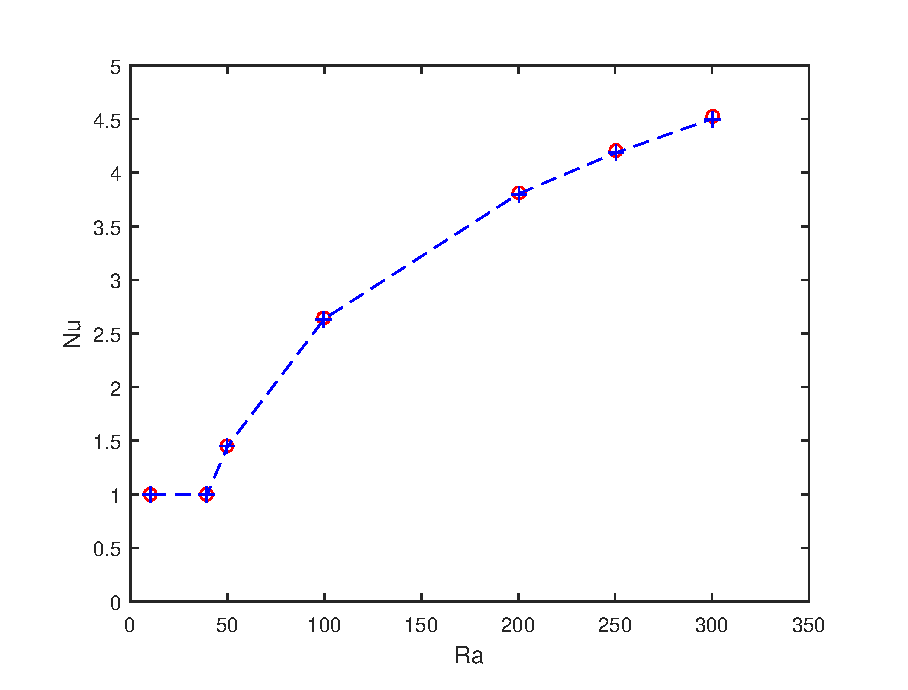
\includegraphics[width = \textwidth]{HRL-Nu-comparison}
	\setlength\figureheight{4cm} 
	\setlength\figurewidth{6cm}
	% This file was created by matlab2tikz.
% Minimal pgfplots version: 1.3
%
%The latest updates can be retrieved from
%  http://www.mathworks.com/matlabcentral/fileexchange/22022-matlab2tikz
%where you can also make suggestions and rate matlab2tikz.
%
\tikzsetnextfilename{HRL-Nu-comparison}
\begin{tikzpicture}

\begin{axis}[%
width=0.95092\figurewidth,
height=\figureheight,
at={(0\figurewidth,0\figureheight)},
scale only axis,
xmin=0,
xmax=350,
xlabel={$Rm$},
ymin=0,
ymax=5,
ylabel={$Nu$},
ylabel style={rotate=-90},
ytick={0,1,2,3,4,5}
]
\addplot [color=red,only marks,mark=o,mark options={solid},forget plot]
  table[row sep=crcr]{%
10	1\\
39.4784176043574	1\\
50	1.45\\
100	2.651\\
200	3.813\\
250	4.199\\
300	4.523\\
};
\addplot [color=blue,dashed,mark=+,mark options={solid},forget plot]
  table[row sep=crcr]{%
10	1\\
39.4784176043574	1\\
50	1.44844\\
100	2.6378\\
200	3.80152\\
250	4.18411\\
300	4.50164\\
};
\end{axis}
\end{tikzpicture}%
	\label{subfig:HRL-Nu-comparison}
\end{subfigure}

\setlength{\belowcaptionskip}{-7pt} % make text closer to caption

\caption{~\subref{subfig:heated-wire-error} The linear relationship between the average fractional error $\left<\Delta T/T_{analytic} \right>$ and $(\Delta r)^2$ is confirmed as a benchmark test of the second order method.~\subref{subfig:HRL-Nu-comparison} The problem of convection in a 2-D planar porous layer heated from below was solved as a further test of the code; here I plot $Nu(Rm)$. The well documented onset of convection was observed at $4 \pi^2$, and the calculated values (blue crosses) were in good agreement with those of~\citet*{caltagirone-75} (red circles).}
\label{fig:code-verification}
\end{figure*}

The equations governing $\theta$ and $\psi$ within the mushy layer were solved using semi-implicit timestepping and second order finite differences in space on a fixed grid using iterative methods. The momentum equation~\eqref{eq:momentum-simplified} was solved by successive over-relaxation (SOR)~\citep*{young-50}, whilst the time dependent heat equation~\eqref{eq:heat-psi} was solved using an Alternating Direction Implicit (ADI) method~\citep*{peaceman-rachford-55} which ensures second order temporal accuracy. A steady state was deemed to have been reached once the time derivatives of $\theta, \psi$ and $a$ were all $< 10^{-5}$. The mixed and Neumann boundary conditions were enforced using a Taylor expansion centered on the grid point adjacent to the boundary in order to maintain second order finite differencing. Further details of the numerical method can be found in~\autoref{app:numerical-method}.

The numerical method was implemented in MATLAB, and the code was written in stages of increasing complexity in order to verify its accuracy. Similarity solutions for an axisymmetric heated wire are presented in ~\citet*[Chapter~5.9]{nield-bejan-06}, using which I verified second order convergence of my code when solving the system;
\begin{eqnarray}
&&(\psi_r/r)_r = -Rm \theta_r, \hspace{5ex} \psi_r \theta_z - \psi_z \theta_r = (r \theta_r)_r, \\
&&\theta = z, \hspace{5ex} u_r = 0 \hspace{5ex} (r=a), \\
&&\theta = 0, \hspace{5ex} u_z = 0 \hspace{5ex} (r=R),
\end{eqnarray}
as demonstrated in figure~\ref{subfig:heated-wire-error}. In order to test both the implementation of Neumann boundary conditions and the coupling of the heat and momentum equations, I also solved for convection in a 2-D planar porous layer heated from below~\citep*{horton-rogers-45,lapwood-48}. I observed the onset of convection at $Rm = 4 \pi^2$, and found my results for $Nu(Ra)$ to be in good agreement with those of~\citet*{caltagirone-75} over a wide range of $Rm$ (see figure~\ref{subfig:HRL-Nu-comparison}).

Finally, once the full set of boundary conditions for flow with brine channels were applied, the steady state solutions were checked to ensure both the interior equations and boundary conditions were satisfied.

\subsection{Free boundaries}
\label{sec:free-boundary-method}

\begin{figure*}[t!]
\centering
\captionsetup[subfigure]{position=top,singlelinecheck=off,justification=raggedright, aboveskip=-12pt,belowskip=0pt}
\begin{subfigure}[t]{.54\linewidth}
       	\centering
       	 \caption{}
       	%\includegraphics[width=\textwidth]{q-dot-grad-theta}
       	\setlength\figureheight{5cm} 
	\setlength\figurewidth{7cm}
	% This file was created by matlab2tikz.
% Minimal pgfplots version: 1.3
%
%The latest updates can be retrieved from
%  http://www.mathworks.com/matlabcentral/fileexchange/22022-matlab2tikz
%where you can also make suggestions and rate matlab2tikz.
%
\definecolor{mycolor1}{rgb}{0.00000,0.44700,0.74100}%
%
\tikzsetnextfilename{q-dot-grad-theta}
\begin{tikzpicture}

\begin{axis}[%
width=0.355\figurewidth,
height=0.38\figureheight,
at={(0.58\figurewidth,0.6\figureheight)},
scale only axis,
xmin=0,
xmax=0.27674,
ymin=-2.5,
ymax=1.5,
xtick pos=left,
ytick pos=left,
xtick={0, 0.135, 0.27}, %0.273894733510139
xticklabels={$0$,$R/2$, $R$},
ticklabel style = {font=\small}
]
\addplot [color=blue,solid,forget plot]
  table[row sep=crcr]{%
0.0338947335101391	0.367905423712806\\
0.0348947335101391	0.458568909558261\\
0.0358947335101391	0.54362006269954\\
0.0368947335101391	0.622987207791767\\
0.0378947335101391	0.696598669490066\\
0.0388947335101391	0.764382772449563\\
0.0398947335101391	0.826267841325381\\
0.0408947335101391	0.882182200772646\\
0.0418947335101391	0.932054175446481\\
0.0428947335101391	0.975812090002011\\
0.0438947335101391	1.01338426909436\\
0.0448947335101391	1.04469903737865\\
0.0458947335101391	1.06968471951001\\
0.0468947335101391	1.08832982529271\\
0.0478947335101391	1.10106468513865\\
0.0488947335101391	1.10851649262425\\
0.0498947335101391	1.11131334529096\\
0.0508947335101391	1.11008334068022\\
0.0518947335101391	1.10545457633347\\
0.0528947335101391	1.09803384875532\\
0.0538947335101391	1.08815722309625\\
0.0548947335101391	1.07597446172246\\
0.0558947335101391	1.06163165461147\\
0.0568947335101391	1.04527489174084\\
0.0578947335101391	1.02705026308811\\
0.0588947335101391	1.00710364283207\\
0.0598947335101391	0.985575516213182\\
0.0608947335101391	0.962600731936591\\
0.0618947335101391	0.93831387335794\\
0.0628947335101391	0.912849523832872\\
0.0638947335101391	0.886342266717029\\
0.0648947335101391	0.85892629433908\\
0.0658947335101391	0.830710515673148\\
0.0668947335101391	0.801763565475956\\
0.0678947335101391	0.772150484063156\\
0.0688947335101391	0.741936311750395\\
0.0698947335101391	0.711186088853324\\
0.0708947335101391	0.67996484019109\\
0.0718947335101391	0.648332065014775\\
0.0728947335101391	0.616333593588825\\
0.0738947335101391	0.584013179280209\\
0.0748947335101391	0.551414575455896\\
0.0758947335101391	0.518581535482857\\
0.0768947335101391	0.485557812727902\\
0.0778947335101391	0.452384227453849\\
0.0788947335101391	0.419090000708542\\
0.0798947335101391	0.385701486659123\\
0.0808947335101391	0.352245039472733\\
0.0818947335101391	0.318747013316515\\
0.0828947335101391	0.285233762357612\\
0.0838947335101391	0.251730708391593\\
0.0848947335101391	0.218257281477936\\
0.0858947335101391	0.184830541605752\\
0.0868947335101391	0.151467542896368\\
0.0878947335101391	0.11818533947111\\
0.0888947335101391	0.0850009854513031\\
0.0898947335101391	0.0519312000572098\\
0.0908947335101391	0.0189890507229108\\
0.0918947335101391	-0.0138146413109307\\
0.0928947335101391	-0.0464690876026115\\
0.0938947335101391	-0.0789634997104283\\
0.0948947335101391	-0.111287089192679\\
0.0958947335101391	-0.143429163862751\\
0.0968947335101391	-0.175381007160977\\
0.0978947335101391	-0.207135754217902\\
0.0988947335101391	-0.238686611599197\\
0.0998947335101391	-0.270026785870529\\
0.100894733510139	-0.301149483597569\\
0.101894733510139	-0.332047933337586\\
0.102894733510139	-0.362716424698298\\
0.103894733510139	-0.393150758369626\\
0.104894733510139	-0.423346850581487\\
0.105894733510139	-0.453300617563795\\
0.106894733510139	-0.483007975546468\\
0.107894733510139	-0.512464843439477\\
0.108894733510139	-0.541667670359542\\
0.109894733510139	-0.570614070262721\\
0.110894733510139	-0.599301811944615\\
0.111894733510139	-0.627728664200821\\
0.112894733510139	-0.655892395826941\\
0.113894733510139	-0.683790775639417\\
0.114894733510139	-0.711421819685844\\
0.115894733510139	-0.738784406108048\\
0.116894733510139	-0.765877600840381\\
0.117894733510139	-0.792700469817192\\
0.118894733510139	-0.819252078972832\\
0.119894733510139	-0.845531494241653\\
0.120894733510139	-0.871537888015299\\
0.121894733510139	-0.897271033325959\\
0.122894733510139	-0.922730913658319\\
0.123894733510139	-0.947917512722513\\
0.124894733510139	-0.972830814228675\\
0.125894733510139	-0.997470801886941\\
0.126894733510139	-1.02183750119395\\
0.127894733510139	-1.04593133127648\\
0.128894733510139	-1.0697529273675\\
0.129894733510139	-1.09330292692817\\
0.130894733510139	-1.11658196741967\\
0.131894733510139	-1.13959068630315\\
0.132894733510139	-1.16232973515664\\
0.133894733510139	-1.18480000719775\\
0.134894733510139	-1.20700259855241\\
0.135894733510139	-1.22893861164291\\
0.136894733510139	-1.25060914889157\\
0.137894733510139	-1.27201531272068\\
0.138894733510139	-1.29315820923189\\
0.139894733510139	-1.3140390816422\\
0.140894733510139	-1.33465934793603\\
0.141894733510139	-1.35502043744681\\
0.142894733510139	-1.37512377950794\\
0.143894733510139	-1.39497080345284\\
0.144894733510139	-1.41456293917992\\
0.145894733510139	-1.43390168663491\\
0.146894733510139	-1.45298868272013\\
0.147894733510139	-1.47182558020167\\
0.148894733510139	-1.49041403184561\\
0.149894733510139	-1.50875569041806\\
0.150894733510139	-1.52685220870145\\
0.151894733510139	-1.54470527040868\\
0.152894733510139	-1.562316654478\\
0.153894733510139	-1.57968815811409\\
0.154894733510139	-1.59682157852164\\
0.155894733510139	-1.61371871290534\\
0.156894733510139	-1.63038135846986\\
0.157894733510139	-1.64681132353297\\
0.158894733510139	-1.66301047157692\\
0.159894733510139	-1.67898068316877\\
0.160894733510139	-1.69472383888074\\
0.161894733510139	-1.71024181928501\\
0.162894733510139	-1.72553650495378\\
0.163894733510139	-1.74060977914888\\
0.164894733510139	-1.75546354714475\\
0.165894733510139	-1.77009972498389\\
0.166894733510139	-1.78452022878223\\
0.167894733510139	-1.7987269746557\\
0.168894733510139	-1.81272187872024\\
0.169894733510139	-1.82650685700368\\
0.170894733510139	-1.84008382426161\\
0.171894733510139	-1.8534546942929\\
0.172894733510139	-1.86662138087312\\
0.173894733510139	-1.87958579777785\\
0.174894733510139	-1.89234985878264\\
0.175894733510139	-1.90491547717336\\
0.176894733510139	-1.91728455175624\\
0.177894733510139	-1.92945896480747\\
0.178894733510139	-1.94144059770118\\
0.179894733510139	-1.95323133181152\\
0.180894733510139	-1.96483304851261\\
0.181894733510139	-1.97624762895068\\
0.182894733510139	-1.98747693506006\\
0.183894733510139	-1.99852279528235\\
0.184894733510139	-2.00938703469543\\
0.185894733510139	-2.02007147837723\\
0.186894733510139	-2.03057795140563\\
0.187894733510139	-2.04090827883103\\
0.188894733510139	-2.0510642677306\\
0.189894733510139	-2.06104767623234\\
0.190894733510139	-2.07086025420912\\
0.191894733510139	-2.0805037515338\\
0.192894733510139	-2.08997991807925\\
0.193894733510139	-2.09929050371834\\
0.194894733510139	-2.10843724463212\\
0.195894733510139	-2.11742181712688\\
0.196894733510139	-2.12624588114648\\
0.197894733510139	-2.13491109663435\\
0.198894733510139	-2.14341912353397\\
0.199894733510139	-2.15177162178877\\
0.200894733510139	-2.15997024233682\\
0.201894733510139	-2.16801657178736\\
0.202894733510139	-2.17591216876616\\
0.203894733510139	-2.18365859178416\\
0.204894733510139	-2.19125739935232\\
0.205894733510139	-2.1987101499816\\
0.206894733510139	-2.20601839711085\\
0.207894733510139	-2.21318363172754\\
0.208894733510139	-2.22020730280732\\
0.209894733510139	-2.22709085854412\\
0.210894733510139	-2.23383574713187\\
0.211894733510139	-2.24044341676451\\
0.212894733510139	-2.24691531333953\\
0.213894733510139	-2.25325282771975\\
0.214894733510139	-2.25945729447266\\
0.215894733510139	-2.26553004561718\\
0.216894733510139	-2.27147241317221\\
0.217894733510139	-2.27728572915667\\
0.218894733510139	-2.28297132484859\\
0.219894733510139	-2.28853048653315\\
0.220894733510139	-2.2939644304442\\
0.221894733510139	-2.29927436675299\\
0.222894733510139	-2.30446150563078\\
0.223894733510139	-2.30952705724882\\
0.224894733510139	-2.31447223167652\\
0.225894733510139	-2.31929820717574\\
0.226894733510139	-2.32400608521033\\
0.227894733510139	-2.32859695588459\\
0.228894733510139	-2.33307190930286\\
0.229894733510139	-2.33743203556944\\
0.230894733510139	-2.34167842478862\\
0.231894733510139	-2.34581214311051\\
0.232894733510139	-2.3498341643511\\
0.233894733510139	-2.35374544008206\\
0.234894733510139	-2.35754692187505\\
0.235894733510139	-2.36123956130174\\
0.236894733510139	-2.36482430993381\\
0.237894733510139	-2.36830211168829\\
0.238894733510139	-2.37167386258383\\
0.239894733510139	-2.37494044015008\\
0.240894733510139	-2.37810272187719\\
0.241894733510139	-2.3811615852553\\
0.242894733510139	-2.38411790777459\\
0.243894733510139	-2.38697254947107\\
0.244894733510139	-2.389726185725\\
0.245894733510139	-2.39237938091293\\
0.246894733510139	-2.39493269789453\\
0.247894733510139	-2.39738669952947\\
0.248894733510139	-2.39974194867741\\
0.249894733510139	-2.40199902306579\\
0.250894733510139	-2.40415879421933\\
0.251894733510139	-2.40622240296012\\
0.252894733510139	-2.40819100006636\\
0.253894733510139	-2.41006573631627\\
0.254894733510139	-2.41184776248806\\
0.255894733510139	-2.41353820526171\\
0.256894733510139	-2.41513709078065\\
0.257894733510139	-2.41664291289349\\
0.258894733510139	-2.41805405202283\\
0.259894733510139	-2.41936888859128\\
0.260894733510139	-2.42058580302144\\
0.261894733510139	-2.42170319171226\\
0.262894733510139	-2.42272230215695\\
0.263894733510139	-2.42365049805549\\
0.264894733510139	-2.42449593399048\\
0.265894733510139	-2.42526676454455\\
0.266894733510139	-2.42597114430029\\
0.267894733510139	-2.42661722784031\\
0.268894733510139	-2.42721316974723\\
0.269894733510139	-2.42776712460366\\
0.270894733510139	-2.4282872469922\\
0.271894733510139	-2.42878169149547\\
0.272894733510139	-2.42925861269607\\
0.273894733510139	-2.42972616517662\\
};
\draw[dashed, draw=black] (axis cs:0,-0.25) rectangle (axis cs:0.137,1.25);
\end{axis}

\begin{axis}[%
width=0.95092\figurewidth,
height=\figureheight,
at={(0\figurewidth,0\figureheight)},
scale only axis,
xmin=0,
xmax=0.137,
xtick={0, 0.04, 0.08, 0.12},
xlabel={$r$},
ymin=-0.25,
ymax=1.25,
ylabel={$\mathbf{q} \cdot \nabla \theta$},
y label style={at={(0.05,0.67)}, rotate={-90}},
scaled ticks=false, 
tick label style={/pgf/number format/fixed},
xtick pos=left,
ytick pos=left
]
\addplot [color=mycolor1,solid,forget plot]
  table[row sep=crcr]{%
0.0338947335101391	0.367905423712806\\
0.0348947335101391	0.458568909558261\\
0.0358947335101391	0.54362006269954\\
0.0368947335101391	0.622987207791767\\
0.0378947335101391	0.696598669490066\\
0.0388947335101391	0.764382772449563\\
0.0398947335101391	0.826267841325381\\
0.0408947335101391	0.882182200772646\\
0.0418947335101391	0.932054175446481\\
0.0428947335101391	0.975812090002011\\
0.0438947335101391	1.01338426909436\\
0.0448947335101391	1.04469903737865\\
0.0458947335101391	1.06968471951001\\
0.0468947335101391	1.08832982529271\\
0.0478947335101391	1.10106468513865\\
0.0488947335101391	1.10851649262425\\
0.0498947335101391	1.11131334529096\\
0.0508947335101391	1.11008334068022\\
0.0518947335101391	1.10545457633347\\
0.0528947335101391	1.09803384875532\\
0.0538947335101391	1.08815722309625\\
0.0548947335101391	1.07597446172246\\
0.0558947335101391	1.06163165461147\\
0.0568947335101391	1.04527489174084\\
0.0578947335101391	1.02705026308811\\
0.0588947335101391	1.00710364283207\\
0.0598947335101391	0.985575516213182\\
0.0608947335101391	0.962600731936591\\
0.0618947335101391	0.93831387335794\\
0.0628947335101391	0.912849523832872\\
0.0638947335101391	0.886342266717029\\
0.0648947335101391	0.85892629433908\\
0.0658947335101391	0.830710515673148\\
0.0668947335101391	0.801763565475956\\
0.0678947335101391	0.772150484063156\\
0.0688947335101391	0.741936311750395\\
0.0698947335101391	0.711186088853324\\
0.0708947335101391	0.67996484019109\\
0.0718947335101391	0.648332065014775\\
0.0728947335101391	0.616333593588825\\
0.0738947335101391	0.584013179280209\\
0.0748947335101391	0.551414575455896\\
0.0758947335101391	0.518581535482857\\
0.0768947335101391	0.485557812727902\\
0.0778947335101391	0.452384227453849\\
0.0788947335101391	0.419090000708542\\
0.0798947335101391	0.385701486659123\\
0.0808947335101391	0.352245039472733\\
0.0818947335101391	0.318747013316515\\
0.0828947335101391	0.285233762357612\\
0.0838947335101391	0.251730708391593\\
0.0848947335101391	0.218257281477936\\
0.0858947335101391	0.184830541605752\\
0.0868947335101391	0.151467542896368\\
0.0878947335101391	0.11818533947111\\
0.0888947335101391	0.0850009854513031\\
0.0898947335101391	0.0519312000572098\\
0.0908947335101391	0.0189890507229108\\
0.0918947335101391	-0.0138146413109307\\
0.0928947335101391	-0.0464690876026115\\
0.0938947335101391	-0.0789634997104283\\
0.0948947335101391	-0.111287089192679\\
0.0958947335101391	-0.143429163862751\\
0.0968947335101391	-0.175381007160977\\
0.0978947335101391	-0.207135754217902\\
0.0988947335101391	-0.238686611599197\\
0.0998947335101391	-0.270026785870529\\
0.100894733510139	-0.301149483597569\\
0.101894733510139	-0.332047933337586\\
0.102894733510139	-0.362716424698298\\
0.103894733510139	-0.393150758369626\\
0.104894733510139	-0.423346850581487\\
0.105894733510139	-0.453300617563795\\
0.106894733510139	-0.483007975546468\\
0.107894733510139	-0.512464843439477\\
0.108894733510139	-0.541667670359542\\
0.109894733510139	-0.570614070262721\\
0.110894733510139	-0.599301811944615\\
0.111894733510139	-0.627728664200821\\
0.112894733510139	-0.655892395826941\\
0.113894733510139	-0.683790775639417\\
0.114894733510139	-0.711421819685844\\
0.115894733510139	-0.738784406108048\\
0.116894733510139	-0.765877600840381\\
0.117894733510139	-0.792700469817192\\
0.118894733510139	-0.819252078972832\\
0.119894733510139	-0.845531494241653\\
0.120894733510139	-0.871537888015299\\
0.121894733510139	-0.897271033325959\\
0.122894733510139	-0.922730913658319\\
0.123894733510139	-0.947917512722513\\
0.124894733510139	-0.972830814228675\\
0.125894733510139	-0.997470801886941\\
0.126894733510139	-1.02183750119395\\
0.127894733510139	-1.04593133127648\\
0.128894733510139	-1.0697529273675\\
0.129894733510139	-1.09330292692817\\
0.130894733510139	-1.11658196741967\\
0.131894733510139	-1.13959068630315\\
0.132894733510139	-1.16232973515664\\
0.133894733510139	-1.18480000719775\\
0.134894733510139	-1.20700259855241\\
0.135894733510139	-1.22893861164291\\
0.136894733510139	-1.25060914889157\\
0.137894733510139	-1.27201531272068\\
0.138894733510139	-1.29315820923189\\
0.139894733510139	-1.3140390816422\\
0.140894733510139	-1.33465934793603\\
0.141894733510139	-1.35502043744681\\
0.142894733510139	-1.37512377950794\\
0.143894733510139	-1.39497080345284\\
0.144894733510139	-1.41456293917992\\
0.145894733510139	-1.43390168663491\\
0.146894733510139	-1.45298868272013\\
0.147894733510139	-1.47182558020167\\
0.148894733510139	-1.49041403184561\\
0.149894733510139	-1.50875569041806\\
0.150894733510139	-1.52685220870145\\
0.151894733510139	-1.54470527040868\\
0.152894733510139	-1.562316654478\\
0.153894733510139	-1.57968815811409\\
0.154894733510139	-1.59682157852164\\
0.155894733510139	-1.61371871290534\\
0.156894733510139	-1.63038135846986\\
0.157894733510139	-1.64681132353297\\
0.158894733510139	-1.66301047157692\\
0.159894733510139	-1.67898068316877\\
0.160894733510139	-1.69472383888074\\
0.161894733510139	-1.71024181928501\\
0.162894733510139	-1.72553650495378\\
0.163894733510139	-1.74060977914888\\
0.164894733510139	-1.75546354714475\\
0.165894733510139	-1.77009972498389\\
0.166894733510139	-1.78452022878223\\
0.167894733510139	-1.7987269746557\\
0.168894733510139	-1.81272187872024\\
0.169894733510139	-1.82650685700368\\
0.170894733510139	-1.84008382426161\\
0.171894733510139	-1.8534546942929\\
0.172894733510139	-1.86662138087312\\
0.173894733510139	-1.87958579777785\\
0.174894733510139	-1.89234985878264\\
0.175894733510139	-1.90491547717336\\
0.176894733510139	-1.91728455175624\\
0.177894733510139	-1.92945896480747\\
0.178894733510139	-1.94144059770118\\
0.179894733510139	-1.95323133181152\\
0.180894733510139	-1.96483304851261\\
0.181894733510139	-1.97624762895068\\
0.182894733510139	-1.98747693506006\\
0.183894733510139	-1.99852279528235\\
0.184894733510139	-2.00938703469543\\
0.185894733510139	-2.02007147837723\\
0.186894733510139	-2.03057795140563\\
0.187894733510139	-2.04090827883103\\
0.188894733510139	-2.0510642677306\\
0.189894733510139	-2.06104767623234\\
0.190894733510139	-2.07086025420912\\
0.191894733510139	-2.0805037515338\\
0.192894733510139	-2.08997991807925\\
0.193894733510139	-2.09929050371834\\
0.194894733510139	-2.10843724463212\\
0.195894733510139	-2.11742181712688\\
0.196894733510139	-2.12624588114648\\
0.197894733510139	-2.13491109663435\\
0.198894733510139	-2.14341912353397\\
0.199894733510139	-2.15177162178877\\
0.200894733510139	-2.15997024233682\\
0.201894733510139	-2.16801657178736\\
0.202894733510139	-2.17591216876616\\
0.203894733510139	-2.18365859178416\\
0.204894733510139	-2.19125739935232\\
0.205894733510139	-2.1987101499816\\
0.206894733510139	-2.20601839711085\\
0.207894733510139	-2.21318363172754\\
0.208894733510139	-2.22020730280732\\
0.209894733510139	-2.22709085854412\\
0.210894733510139	-2.23383574713187\\
0.211894733510139	-2.24044341676451\\
0.212894733510139	-2.24691531333953\\
0.213894733510139	-2.25325282771975\\
0.214894733510139	-2.25945729447266\\
0.215894733510139	-2.26553004561718\\
0.216894733510139	-2.27147241317221\\
0.217894733510139	-2.27728572915667\\
0.218894733510139	-2.28297132484859\\
0.219894733510139	-2.28853048653315\\
0.220894733510139	-2.2939644304442\\
0.221894733510139	-2.29927436675299\\
0.222894733510139	-2.30446150563078\\
0.223894733510139	-2.30952705724882\\
0.224894733510139	-2.31447223167652\\
0.225894733510139	-2.31929820717574\\
0.226894733510139	-2.32400608521033\\
0.227894733510139	-2.32859695588459\\
0.228894733510139	-2.33307190930286\\
0.229894733510139	-2.33743203556944\\
0.230894733510139	-2.34167842478862\\
0.231894733510139	-2.34581214311051\\
0.232894733510139	-2.3498341643511\\
0.233894733510139	-2.35374544008206\\
0.234894733510139	-2.35754692187505\\
0.235894733510139	-2.36123956130174\\
0.236894733510139	-2.36482430993381\\
0.237894733510139	-2.36830211168829\\
0.238894733510139	-2.37167386258383\\
0.239894733510139	-2.37494044015008\\
0.240894733510139	-2.37810272187719\\
0.241894733510139	-2.3811615852553\\
0.242894733510139	-2.38411790777459\\
0.243894733510139	-2.38697254947107\\
0.244894733510139	-2.389726185725\\
0.245894733510139	-2.39237938091293\\
0.246894733510139	-2.39493269789453\\
0.247894733510139	-2.39738669952947\\
0.248894733510139	-2.39974194867741\\
0.249894733510139	-2.40199902306579\\
0.250894733510139	-2.40415879421933\\
0.251894733510139	-2.40622240296012\\
0.252894733510139	-2.40819100006636\\
0.253894733510139	-2.41006573631627\\
0.254894733510139	-2.41184776248806\\
0.255894733510139	-2.41353820526171\\
0.256894733510139	-2.41513709078065\\
0.257894733510139	-2.41664291289349\\
0.258894733510139	-2.41805405202283\\
0.259894733510139	-2.41936888859128\\
0.260894733510139	-2.42058580302144\\
0.261894733510139	-2.42170319171226\\
0.262894733510139	-2.42272230215695\\
0.263894733510139	-2.42365049805549\\
0.264894733510139	-2.42449593399048\\
0.265894733510139	-2.42526676454455\\
0.266894733510139	-2.42597114430029\\
0.267894733510139	-2.42661722784031\\
0.268894733510139	-2.42721316974723\\
0.269894733510139	-2.42776712460366\\
0.270894733510139	-2.4282872469922\\
0.271894733510139	-2.42878169149547\\
0.272894733510139	-2.42925861269607\\
0.273894733510139	-2.42972616517662\\
};
\addplot [color=red,dashed,forget plot]
  table[row sep=crcr]{%
0	-2.70510926811916\\
0.001	-2.61444578227371\\
0.002	-2.52378229642825\\
0.003	-2.4331188105828\\
0.004	-2.34245532473734\\
0.005	-2.25179183889189\\
0.006	-2.16112835304643\\
0.007	-2.07046486720098\\
0.008	-1.97980138135552\\
0.009	-1.88913789551007\\
0.01	-1.79847440966461\\
0.011	-1.70781092381916\\
0.012	-1.6171474379737\\
0.013	-1.52648395212825\\
0.014	-1.43582046628279\\
0.015	-1.34515698043734\\
0.016	-1.25449349459188\\
0.017	-1.16383000874643\\
0.018	-1.07316652290097\\
0.019	-0.982503037055517\\
0.02	-0.891839551210062\\
0.021	-0.801176065364607\\
0.022	-0.710512579519152\\
0.023	-0.619849093673697\\
0.024	-0.529185607828242\\
0.025	-0.438522121982787\\
0.026	-0.347858636137332\\
0.027	-0.257195150291877\\
0.028	-0.166531664446422\\
0.029	-0.0758681786009669\\
0.03	0.0147953072444882\\
0.031	0.105458793089943\\
0.032	0.196122278935398\\
0.033	0.286785764780853\\
0.034	0.377449250626308\\
};
\addplot [color=white!70!black,solid,forget plot]
  table[row sep=crcr]{%
0.0338947335101391	-0.5\\
0.0338947335101391	0.367905423712806\\
};
\addplot [color=gray,solid,forget plot]
  table[row sep=crcr]{%
0.0298368107391138	-0.5\\
0.0298368107391138	0\\
};
\addplot [color=black,solid,forget plot]
  table[row sep=crcr]{%
0	0\\
0.01	0\\
0.02	0\\
0.03	0\\
0.04	0\\
0.05	0\\
0.06	0\\
0.07	0\\
0.08	0\\
0.09	0\\
0.1	0\\
0.11	0\\
0.12	0\\
0.13	0\\
0.14	0\\
0.15	0\\
0.16	0\\
0.17	0\\
0.18	0\\
0.19	0\\
0.2	0\\
0.21	0\\
0.22	0\\
0.23	0\\
0.24	0\\
0.25	0\\
0.26	0\\
0.27	0\\
};
\addplot [color=red,dashed,forget plot]
  table[row sep=crcr]{%
0	-0.0770265034778732\\
0.001	-0.0520408213465116\\
0.002	-0.0270551392151499\\
0.003	-0.00206945708378825\\
0.004	0.0229162250475734\\
0.005	0.0479019071789349\\
0.006	0.0728875893102966\\
0.007	0.0978732714416582\\
0.008	0.12285895357302\\
0.009	0.147844635704382\\
0.01	0.172830317835743\\
0.011	0.197815999967105\\
0.012	0.222801682098467\\
0.013	0.247787364229828\\
0.014	0.27277304636119\\
0.015	0.297758728492551\\
0.016	0.322744410623913\\
0.017	0.347730092755275\\
0.018	0.372715774886637\\
0.019	0.397701457017998\\
0.02	0.42268713914936\\
0.021	0.447672821280722\\
0.022	0.472658503412083\\
0.023	0.497644185543445\\
0.024	0.522629867674806\\
0.025	0.547615549806168\\
0.026	0.57260123193753\\
0.027	0.597586914068891\\
0.028	0.622572596200253\\
0.029	0.647558278331615\\
0.03	0.672543960462976\\
0.031	0.697529642594338\\
0.032	0.7225153247257\\
0.033	0.747501006857061\\
0.034	0.772486688988423\\
0.035	0.797472371119784\\
0.036	0.822458053251146\\
0.037	0.847443735382508\\
0.038	0.872429417513869\\
0.039	0.897415099645231\\
0.04	0.922400781776593\\
0.041	0.947386463907954\\
0.042	0.972372146039316\\
0.043	0.997357828170678\\
0.044	1.02234351030204\\
0.045	1.0473291924334\\
};
\addplot [color=white!70!black,solid,forget plot]
  table[row sep=crcr]{%
0.0448947335101391	-0.5\\
0.0448947335101391	1.04469903737865\\
};
\addplot [color=gray,solid,forget plot]
  table[row sep=crcr]{%
0.00308282571886204	-0.5\\
0.00308282571886204	0\\
};
\addplot [color=black,solid,forget plot]
  table[row sep=crcr]{%
0	0\\
0.01	0\\
0.02	0\\
0.03	0\\
0.04	0\\
0.05	0\\
0.06	0\\
0.07	0\\
0.08	0\\
0.09	0\\
0.1	0\\
0.11	0\\
0.12	0\\
0.13	0\\
0.14	0\\
0.15	0\\
0.16	0\\
0.17	0\\
0.18	0\\
0.19	0\\
0.2	0\\
0.21	0\\
0.22	0\\
0.23	0\\
0.24	0\\
0.25	0\\
0.26	0\\
0.27	0\\
};
\end{axis}
\end{tikzpicture}%
       	\label{subfig:q-dot-grad-theta}
\end{subfigure}
\quad
\captionsetup[subfigure]{aboveskip=-18pt}
\begin{subfigure}[t]{.42\linewidth}
       	\centering
        	\caption{}
      	% \includegraphics[width=\textwidth]{q-dot-grad-theta-root}
      	\setlength\figureheight{5cm} 
	\setlength\figurewidth{4cm}
	\input{q-dot-grad-theta-root.tikz}
    	\label{subfig:q-dot-grad-theta-root}
\end{subfigure}

\setlength{\belowcaptionskip}{-7pt} % make text closer to caption

\caption{~\subref{subfig:q-dot-grad-theta} Cross section of $\mathbf{q} \cdot \nabla \theta$, taken at $z=-2H/3$. The full curve is plotted in the top right corner, with the region in the dashed box magnified to produce the main plot. Dashed red lines are linear extrapolations from two points on the curve separated by $\Delta r = 0.04R$. The large variation in the roots of these extrapolations illustrates the sensitivity of this method, which makes it infeasible.~\subref{subfig:q-dot-grad-theta-root} $ \left. \mathbf{q} \cdot \nabla \theta \right|_{r=a}$ calculated for steady state solutions with $a=b$. The negative gradient at the root $ \left. \mathbf{q} \cdot \nabla \theta \right|_{r=a} = 0$ motivates the implementation of the relaxation method given in equation~\eqref{eq:relaxation-q-dot-grad-theta}. }
\label{fig:free-boundary-method}  

\end{figure*}

Implementing the condition of marginal equilibrium~\eqref{eq:chimney-bc} at the chimney wall posed significant difficulty. I chose to apply it at $z = - 2H/3$, where the straight sided approximation should be most accurate; near the solid-mush boundary the chimney width is observed to decrease and may in fact disappear altogether, whilst the singularity at the mush-ocean boundary means that the local values of $\theta$ and $\psi$ are unreliable. To enforce this condition, it is necessary to extrapolate from $r=b$ at each time step and then adjust $a$ appropriately. 

A first attempt was made using a linear extrapolation for $f(r) = \mathbf{q} \cdot \nabla \theta$,
\begin{equation}
f(a) = f(b) + (a-b) \left. \frac{\partial f}{\partial r}\right|_{r=b} \, ,
\end{equation}
and solving for the root $f(a)=0$ to find a new estimate for the chimney radius $a^*$. The chimney radius $a(t)$ was then updated by relaxing towards $a^*$,
\begin{equation}
\frac{da}{dt} = \lambda (a - a^*),
\end{equation}
with constant $\lambda$. However this produced an unstable scheme in which the chimney width often became zero, as the extrapolation was highly sensitive to the position of $b$ on the $\mathbf{q} \cdot \nabla \theta$ curve (see figure~\ref{subfig:q-dot-grad-theta}).

A more careful analysis revealed that, based on the form of $\psi$ and $\theta$ in the region $a < r < b$ derived in~\autoref{sec:patching-equations}, the Pad\'{e} approximation
\begin{equation}
\mathbf{q} \cdot \nabla \theta \approx \frac{c_1 r^3 + c_2 r^2 + c_3 r + c_4}{r}
\end{equation}
might be more appropriate for extrapolation, where $c_1, c_2, c_3$ and $c_4$ are fitted from data at the edge of the computational grid. However this too was found to be unstable, in this case due to the $1/r$ term causing the extrapolation to, in some cases, predict no roots at all. Removing the $1/r$ term and instead considering a quadratic function with $c_4=0$ was slightly more successful, but the predicted chimney radii $a^*$ were still highly dependant on the form of $\mathbf{q} \cdot \nabla \theta$ at $r=b$ and convergence to a steady state with chimneys could not be achieved.

By fixing $a=b$ and finding steady states at a range of chimney widths, I saw that $\left. \mathbf{q} \cdot \nabla \theta \right|_{r=a}$ approaches a root from above as $a$ increases (figure~\ref{subfig:q-dot-grad-theta-root}). This suggested a new relaxation scheme:
\begin{equation}
\label{eq:relaxation-q-dot-grad-theta}
\frac{da}{dt} = \lambda \left. \mathbf{q} \cdot \nabla \theta \right|_{r=a}
\end{equation}
where $\left. \mathbf{q} \cdot \nabla \theta \right|_{r=a}$ was calculated using a quadratic extrapolation from $r=b$, and the relaxation parameter $\lambda = 0.002$ was chosen empirically. Using this method it was possible to converge on a steady state with chimneys, so the description of the numerical scheme is complete.


\section{Numerical results and their interpretation}
\label{sec:results}

\begin{figure*}[t!]
\centering
\captionsetup[subfigure]{position=top,singlelinecheck=off,justification=raggedright, aboveskip=-14pt,belowskip=0pt}
\begin{subfigure}[t]{.48\linewidth}
	\centering
    	%\includegraphics[width=0.9\textwidth]{steady-state-Rm60H0-25R0-25}
   	\setlength\figureheight{5cm} 
	\setlength\figurewidth{6.5cm}
	\caption{}
	% This file was created by matlab2tikz.
% Minimal pgfplots version: 1.3
%
%The latest updates can be retrieved from
%  http://www.mathworks.com/matlabcentral/fileexchange/22022-matlab2tikz
%where you can also make suggestions and rate matlab2tikz.
%
\begin{tikzpicture}

\begin{axis}[%
width=0.95092\figurewidth,
height=\figureheight,
at={(0\figurewidth,0\figureheight)},
scale only axis,
xmin=0,
xmax=0.24953768,
xlabel={r},
ymin=-0.25,
ymax=-0,
ylabel={z}
]
\addplot[contour prepared, contour prepared format=matlab, contour/labels=false] table[row sep=crcr] {%
%
-0.909090909090927	384\\
0	-0.02531141689945\\
0.00065324	-0.02531141689945\\
0.00130648	-0.02531141689945\\
0.00195972	-0.02531141689945\\
0.00261296	-0.02531141689945\\
0.0032662	-0.02531141689945\\
0.00391944	-0.02531141689945\\
0.00457268	-0.02531141689945\\
0.00522592	-0.02531141689945\\
0.00587916	-0.02531141689945\\
0.0065324	-0.02531141689945\\
0.00718564	-0.02531141689945\\
0.00783888	-0.02531141689945\\
0.00849212	-0.02531141689945\\
0.00914536	-0.02531141689945\\
0.0097986	-0.02531141689945\\
0.01045184	-0.02531141689945\\
0.01110508	-0.02531141689945\\
0.01175832	-0.02531141689945\\
0.01241156	-0.02531141689945\\
0.0130648	-0.02531141689945\\
0.01371804	-0.02531141689945\\
0.01437128	-0.02531141689945\\
0.01502452	-0.02531141689945\\
0.01567776	-0.02531141689945\\
0.016331	-0.02531141689945\\
0.01698424	-0.02531141689945\\
0.01763748	-0.02531141689945\\
0.01829072	-0.02531141689945\\
0.01894396	-0.02531141689945\\
0.0195972	-0.02531141689945\\
0.02025044	-0.02531141689945\\
0.02090368	-0.02531141689945\\
0.02155692	-0.02531141689945\\
0.02221016	-0.02531141689945\\
0.0228634	-0.02531141689945\\
0.02351664	-0.02531141689945\\
0.02416988	-0.02531141689945\\
0.02482312	-0.02531141689945\\
0.02547636	-0.02531141689945\\
0.0261296	-0.02531141689945\\
0.02678284	-0.02531141689945\\
0.02743608	-0.02531141689945\\
0.02808932	-0.02531141689945\\
0.02874256	-0.02531141689945\\
0.0293958	-0.02531141689945\\
0.03004904	-0.02531141689945\\
0.03070228	-0.02531141689945\\
0.03135552	-0.02531141689945\\
0.03200876	-0.02531141689945\\
0.032662	-0.02531141689945\\
0.03331524	-0.0252219781853974\\
0.03396848	-0.0251348128688869\\
0.03462172	-0.0250498331176618\\
0.03527496	-0.0249669541070649\\
0.0359282	-0.0248860938576321\\
0.03658144	-0.0248071730827509\\
0.03723468	-0.0247301150457023\\
0.03788792	-0.0246548454254626\\
0.03854116	-0.0245812921906891\\
0.0391944	-0.0245093854813606\\
0.03984764	-0.0244390574975846\\
0.04050088	-0.0243702423951197\\
0.04115412	-0.0243028761871982\\
0.04180736	-0.0242368966522662\\
0.0424606	-0.0241722432472827\\
0.04311384	-0.0241088570262533\\
0.04376708	-0.024046680563692\\
0.04442032	-0.0239856604032066\\
0.04507356	-0.0239257565096802\\
0.0457268	-0.023866933514673\\
0.04638004	-0.0238091569860852\\
0.04703328	-0.0237523933880126\\
0.04768652	-0.0236966100433341\\
0.04833976	-0.0236417750981964\\
0.048993	-0.0235878574882999\\
0.04964624	-0.023534826963398\\
0.05029948	-0.0234826560909034\\
0.05095272	-0.0234313207239652\\
0.05160596	-0.0233807974249084\\
0.0522592	-0.0233310632698662\\
0.05291244	-0.0232820958301155\\
0.05356568	-0.0232338731542323\\
0.05421892	-0.0231863737510269\\
0.05487216	-0.0231395765732281\\
0.0555254	-0.0230934614398066\\
0.05617864	-0.0230480111096344\\
0.05683188	-0.0230032095911307\\
0.05748512	-0.022959041204095\\
0.05813836	-0.0229154905685207\\
0.0587916	-0.0228725425950327\\
0.05944484	-0.0228301824756883\\
0.06009808	-0.0227883956751298\\
0.06075132	-0.0227471679369399\\
0.06140456	-0.0227064860768816\\
0.0620578	-0.0226663383633263\\
0.06271104	-0.0226267133666982\\
0.06336428	-0.0225875998516974\\
0.06401752	-0.0225489867717422\\
0.06467076	-0.0225108632635985\\
0.065324	-0.0224732186421903\\
0.06597724	-0.0224360423955856\\
0.06663048	-0.022399324315064\\
0.06728372	-0.0223630553023081\\
0.06793696	-0.0223272268076872\\
0.0685902	-0.0222918304145264\\
0.06924344	-0.0222568578340835\\
0.06989668	-0.022222300902238\\
0.07054992	-0.0221881515762808\\
0.07120316	-0.0221544019317998\\
0.0718564	-0.0221210441635008\\
0.07250964	-0.0220880709190439\\
0.07316288	-0.0220554755528314\\
0.07381612	-0.022023251574457\\
0.07446936	-0.0219913925840061\\
0.0751226	-0.0219598922699013\\
0.07577584	-0.0219287444068076\\
0.07642908	-0.0218979428535942\\
0.07708232	-0.0218674815513518\\
0.07773556	-0.021837354572578\\
0.0783888	-0.0218075565077077\\
0.07904204	-0.0217780822422199\\
0.07969528	-0.0217489267295651\\
0.08034852	-0.0217200849878722\\
0.08100176	-0.0216915520985243\\
0.081655	-0.0216633232047697\\
0.08230824	-0.0216353935103675\\
0.08296148	-0.0216077582792043\\
0.08361472	-0.0215804129864439\\
0.08426796	-0.0215533534837618\\
0.0849212	-0.0215265757135429\\
0.08557444	-0.0215000756668935\\
0.08622768	-0.0214738493826376\\
0.08688092	-0.0214478929463353\\
0.08753416	-0.0214222024893253\\
0.0881874	-0.0213967741877879\\
0.08884064	-0.0213716042826525\\
0.08949388	-0.0213466892795069\\
0.09014712	-0.0213220258576734\\
0.09080036	-0.0212976107359732\\
0.0914536	-0.0212734406701118\\
0.09210684	-0.0212495124519643\\
0.09276008	-0.0212258229088768\\
0.09341332	-0.0212023689029818\\
0.09406656	-0.0211791473307186\\
0.0947198	-0.0211561551941677\\
0.09537304	-0.0211333897078234\\
0.09602628	-0.0211108481437831\\
0.09667952	-0.0210885278032675\\
0.09733276	-0.0210664260160855\\
0.097986	-0.0210445401401106\\
0.09863924	-0.0210228675607671\\
0.09929248	-0.0210014056905277\\
0.09994572	-0.0209801519771201\\
0.10059896	-0.0209591040106298\\
0.1012522	-0.0209382594886416\\
0.10190544	-0.0209176161339726\\
0.10255868	-0.0208971716924592\\
0.10321192	-0.0208769239325547\\
0.10386516	-0.0208568706449359\\
0.1045184	-0.0208370096421148\\
0.10517164	-0.0208173387580843\\
0.10582488	-0.0207978558827875\\
0.10647812	-0.0207785590308057\\
0.10713136	-0.0207594462554074\\
0.1077846	-0.020740515628699\\
0.10843784	-0.0207217652413108\\
0.10909108	-0.0207031932020866\\
0.10974432	-0.0206847976377807\\
0.11039756	-0.0206665766927586\\
0.1110508	-0.020648528532375\\
0.11170404	-0.0206306514018226\\
0.11235728	-0.0206129436153029\\
0.11301052	-0.0205954035043022\\
0.11366376	-0.0205780294156915\\
0.114317	-0.0205608197114787\\
0.11497024	-0.020543772768566\\
0.11562348	-0.0205268869785108\\
0.11627672	-0.0205101607472912\\
0.11692996	-0.0204935925123561\\
0.1175832	-0.0204771807870564\\
0.11823644	-0.0204609241118947\\
0.11888968	-0.0204448210403064\\
0.11954292	-0.0204288701384589\\
0.12019616	-0.0204130699850542\\
0.1208494	-0.0203974191711343\\
0.12150264	-0.0203819162998899\\
0.12215588	-0.020366559988035\\
0.12280912	-0.0203513488991853\\
0.12346236	-0.0203362817430013\\
0.1241156	-0.0203213572416097\\
0.12476884	-0.0203065741279552\\
0.12542208	-0.0202919311456378\\
0.12607532	-0.0202774270487524\\
0.12672856	-0.0202630606017308\\
0.1273818	-0.0202488305791862\\
0.12803504	-0.0202347357746712\\
0.12868828	-0.0202207750301017\\
0.12934152	-0.0202069472072749\\
0.12999476	-0.0201932511772591\\
0.130648	-0.0201796858202576\\
0.13130124	-0.0201662500254745\\
0.13195448	-0.0201529426909832\\
0.13260772	-0.0201397627235959\\
0.13326096	-0.0201267090394138\\
0.1339142	-0.0201137805837586\\
0.13456744	-0.0201009763342644\\
0.13522068	-0.0200882952779229\\
0.13587392	-0.0200757364096117\\
0.13652716	-0.0200632987319818\\
0.1371804	-0.0200509812553463\\
0.13783364	-0.0200387829975704\\
0.13848688	-0.020026702983963\\
0.13914012	-0.020014740252066\\
0.13979336	-0.0200028938721554\\
0.1404466	-0.0199911629297847\\
0.14109984	-0.0199795465173588\\
0.14175308	-0.019968043734033\\
0.14240632	-0.0199566536856185\\
0.14305956	-0.0199453754844891\\
0.1437128	-0.0199342082494886\\
0.14436604	-0.0199231511061426\\
0.14501928	-0.0199122031994791\\
0.14567252	-0.0199013636987111\\
0.14632576	-0.0198906317803283\\
0.146979	-0.0198800066267091\\
0.14763224	-0.0198694874260396\\
0.14828548	-0.0198590733722336\\
0.14893872	-0.0198487636648532\\
0.14959196	-0.0198385575090309\\
0.1502452	-0.0198284541183196\\
0.15089844	-0.0198184527301484\\
0.15155168	-0.0198085525943859\\
0.15220492	-0.0197987529660723\\
0.15285816	-0.0197890531053331\\
0.1535114	-0.0197794522773096\\
0.15416464	-0.019769949752091\\
0.15481788	-0.019760544804647\\
0.15547112	-0.0197512367148989\\
0.15612436	-0.0197420247767361\\
0.1567776	-0.0197329083035439\\
0.15743084	-0.0197238866145828\\
0.15808408	-0.0197149590335778\\
0.15873732	-0.0197061248886583\\
0.15939056	-0.0196973835122992\\
0.1600438	-0.019688734241262\\
0.16069704	-0.0196801764165379\\
0.16135028	-0.0196717093851982\\
0.16200352	-0.0196633325130824\\
0.16265676	-0.0196550451768274\\
0.16331	-0.0196468467570349\\
0.16396324	-0.0196387366381817\\
0.16461648	-0.0196307142085687\\
0.16526972	-0.0196227788602699\\
0.16592296	-0.0196149299890819\\
0.1665762	-0.0196071669945366\\
0.16722944	-0.0195994892867819\\
0.16788268	-0.0195918962928394\\
0.16853592	-0.0195843874446901\\
0.16918916	-0.0195769621777301\\
0.1698424	-0.0195696199307256\\
0.17049564	-0.0195623601457681\\
0.17114888	-0.0195551822682313\\
0.17180212	-0.0195480857467273\\
0.17245536	-0.0195410700343912\\
0.1731086	-0.0195341346000331\\
0.17376184	-0.0195272789224211\\
0.17441508	-0.019520502483407\\
0.17506832	-0.0195138047678163\\
0.17572156	-0.0195071852634093\\
0.1763748	-0.0195006434608424\\
0.17702804	-0.0194941788536305\\
0.17768128	-0.0194877909381345\\
0.17833452	-0.0194814792191043\\
0.17898776	-0.0194752432167032\\
0.179641	-0.0194690824555021\\
0.18029424	-0.0194629964626979\\
0.18094748	-0.0194569847680798\\
0.18160072	-0.0194510469039949\\
0.18225396	-0.0194451824053162\\
0.1829072	-0.0194393908094088\\
0.18356044	-0.0194336716570502\\
0.18421368	-0.0194280245026167\\
0.18486692	-0.0194224489101108\\
0.18552016	-0.0194169444459801\\
0.1861734	-0.0194115106789629\\
0.18682664	-0.0194061471800596\\
0.18747988	-0.0194008535225037\\
0.18813312	-0.0193956292817325\\
0.18878636	-0.0193904740353666\\
0.1894396	-0.0193853873677723\\
0.19009284	-0.0193803688778358\\
0.19074608	-0.0193754181685735\\
0.19139932	-0.019370534845029\\
0.19205256	-0.0193657185142473\\
0.1927058	-0.0193609687852495\\
0.19335904	-0.0193562852690077\\
0.19401228	-0.0193516675784196\\
0.19466552	-0.0193471153289655\\
0.19531876	-0.0193426281481072\\
0.195972	-0.019338205672876\\
0.19662524	-0.0193338475422956\\
0.19727848	-0.0193295533971626\\
0.19793172	-0.0193253228800241\\
0.19858496	-0.0193211556351559\\
0.1992382	-0.0193170513085407\\
0.19989144	-0.0193130095478472\\
0.20054468	-0.0193090300061697\\
0.20119792	-0.0193051123504088\\
0.20185116	-0.0193012562515179\\
0.2025044	-0.0192974613820226\\
0.20315764	-0.0192937274160017\\
0.20381088	-0.0192900540290679\\
0.20446412	-0.0192864408983482\\
0.20511736	-0.0192828877024657\\
0.2057706	-0.0192793941219923\\
0.20642384	-0.0192759598480139\\
0.20707708	-0.019272584581199\\
0.20773032	-0.0192692680239051\\
0.20838356	-0.0192660098798704\\
0.2090368	-0.0192628098541963\\
0.20969004	-0.0192596676533314\\
0.21034328	-0.0192565829850541\\
0.21099652	-0.0192535555584571\\
0.21164976	-0.0192505850869722\\
0.212303	-0.0192476712971462\\
0.21295624	-0.0192448139196535\\
0.21360948	-0.0192420126863978\\
0.21426272	-0.0192392673304978\\
0.21491596	-0.0192365775862725\\
0.2155692	-0.0192339431892268\\
0.21622244	-0.0192313638760373\\
0.216376296152621	-0.0192307692307692\\
0.21687568	-0.0192288532543998\\
0.21752892	-0.0192264010912803\\
0.21818216	-0.0192240028717407\\
0.2188354	-0.0192216583548782\\
0.21948864	-0.0192193673008823\\
0.22014188	-0.0192171294710224\\
0.22079512	-0.0192149446276347\\
0.22144836	-0.0192128125341104\\
0.2221016	-0.0192107329548828\\
0.22275484	-0.0192087056580532\\
0.22340808	-0.0192067304251076\\
0.22406132	-0.0192048070421484\\
0.22471456	-0.0192029352962595\\
0.2253678	-0.0192011149754946\\
0.22602104	-0.0191993458688667\\
0.22667428	-0.0191976277663367\\
0.22732752	-0.0191959604588032\\
0.22798076	-0.0191943437381998\\
0.228634	-0.0191927774012164\\
0.22928724	-0.0191912612502231\\
0.22994048	-0.0191897950887735\\
0.23059372	-0.0191883787212957\\
0.23124696	-0.0191870119530828\\
0.2319002	-0.0191856945902838\\
0.23255344	-0.0191844264398946\\
0.23320668	-0.0191832073097484\\
0.23385992	-0.0191820370130755\\
0.23451316	-0.0191809153897819\\
0.2351664	-0.0191798422896728\\
0.23581964	-0.0191788175633672\\
0.23647288	-0.0191778410622784\\
0.23712612	-0.0191769126386059\\
0.23777936	-0.0191760321453257\\
0.2384326	-0.0191751994361819\\
0.23908584	-0.0191744143649426\\
0.23973908	-0.0191736767479802\\
0.24039232	-0.0191729863464834\\
0.24104556	-0.0191723429179248\\
0.2416988	-0.019171746220508\\
0.24235204	-0.0191711960131572\\
0.24300528	-0.0191706920555077\\
0.24365852	-0.0191702341078962\\
0.24431176	-0.0191698219313513\\
0.244965	-0.019169455287584\\
0.24561824	-0.0191691339389778\\
0.24627148	-0.0191688576485801\\
0.24692472	-0.019168626180092\\
0.24757796	-0.0191684392978599\\
0.2482312	-0.0191682967668654\\
0.24888444	-0.0191681983527168\\
0.24953768	-0.0191681438216399\\
-0.818181818181835	385\\
0	-0.0513669209890937\\
0.00065324	-0.0513669209890937\\
0.00130648	-0.0513669209890937\\
0.00195972	-0.0513669209890937\\
0.00261296	-0.0513669209890937\\
0.0032662	-0.0513669209890937\\
0.00391944	-0.0513669209890937\\
0.00457268	-0.0513669209890937\\
0.00522592	-0.0513669209890937\\
0.00587916	-0.0513669209890937\\
0.0065324	-0.0513669209890937\\
0.00718564	-0.0513669209890937\\
0.00783888	-0.0513669209890937\\
0.00849212	-0.0513669209890937\\
0.00914536	-0.0513669209890937\\
0.0097986	-0.0513669209890937\\
0.01045184	-0.0513669209890937\\
0.01110508	-0.0513669209890937\\
0.01175832	-0.0513669209890937\\
0.01241156	-0.0513669209890937\\
0.0130648	-0.0513669209890937\\
0.01371804	-0.0513669209890937\\
0.01437128	-0.0513669209890937\\
0.01502452	-0.0513669209890937\\
0.01567776	-0.0513669209890937\\
0.016331	-0.0513669209890937\\
0.01698424	-0.0513669209890937\\
0.01763748	-0.0513669209890937\\
0.01829072	-0.0513669209890937\\
0.01894396	-0.0513669209890937\\
0.0195972	-0.0513669209890937\\
0.02025044	-0.0513669209890937\\
0.02090368	-0.0513669209890937\\
0.02155692	-0.0513669209890937\\
0.02221016	-0.0513669209890937\\
0.0228634	-0.0513669209890937\\
0.02351664	-0.0513669209890937\\
0.02416988	-0.0513669209890937\\
0.02482312	-0.0513669209890937\\
0.02547636	-0.0513669209890937\\
0.0261296	-0.0513669209890937\\
0.02678284	-0.0513669209890937\\
0.02743608	-0.0513669209890937\\
0.02808932	-0.0513669209890937\\
0.02874256	-0.0513669209890937\\
0.0293958	-0.0513669209890937\\
0.03004904	-0.0513669209890937\\
0.03070228	-0.0513669209890937\\
0.03135552	-0.0513669209890937\\
0.03200876	-0.0513669209890937\\
0.032662	-0.0513669209890937\\
0.0329526715699219	-0.0512820512820513\\
0.03331524	-0.0511769996280803\\
0.03396848	-0.0509922899266345\\
0.03462172	-0.0508122725954279\\
0.03527496	-0.0506367731895102\\
0.0359282	-0.0504656226529613\\
0.03658144	-0.0502986570433236\\
0.03723468	-0.0501357172721092\\
0.03788792	-0.0499766488603746\\
0.03854116	-0.0498213017084318\\
0.0391944	-0.0496695298788348\\
0.03984764	-0.0495211913918416\\
0.04050088	-0.0493761480326149\\
0.04115412	-0.0492342651694759\\
0.04180736	-0.049095411582575\\
0.0424606	-0.048959459302391\\
0.04311384	-0.0488262834575117\\
0.04376708	-0.0486957621311848\\
0.04442032	-0.0485677812835978\\
0.04507356	-0.0484422537096319\\
0.0457268	-0.0483191014482993\\
0.04638004	-0.0481982483012377\\
0.04703328	-0.0480796197605509\\
0.04768652	-0.0479631429414267\\
0.04833976	-0.0478487465179083\\
0.048993	-0.0477363606616719\\
0.04964624	-0.0476259171139118\\
0.05029948	-0.0475173538342176\\
0.05095272	-0.0474106161731908\\
0.05160596	-0.0473056509820172\\
0.0522592	-0.0472024061687384\\
0.05291244	-0.0471008306602726\\
0.05356568	-0.0470008743660515\\
0.05421892	-0.0469024881432028\\
0.05487216	-0.0468056237632146\\
0.0555254	-0.0467102349647369\\
0.05617864	-0.0466162826082902\\
0.05683188	-0.0465237305211288\\
0.05748512	-0.0464325431827329\\
0.05813836	-0.0463426857009486\\
0.0587916	-0.0462541237919843\\
0.05944484	-0.0461668237611557\\
0.06009808	-0.0460807524843508\\
0.06075132	-0.0459958774276682\\
0.06140456	-0.0459121686534361\\
0.0620578	-0.0458295997984229\\
0.06271104	-0.0457481451847884\\
0.06336428	-0.0456677795507614\\
0.06401752	-0.0455884780385959\\
0.06467076	-0.0455102161829333\\
0.065324	-0.0454329698995571\\
0.06597724	-0.0453567154745268\\
0.06663048	-0.0452814298926782\\
0.06728372	-0.0452070928705435\\
0.06793696	-0.0451336854538678\\
0.0685902	-0.0450611889758311\\
0.06924344	-0.0449895850455047\\
0.06989668	-0.0449188555405788\\
0.0703364335138554	-0.0448717948717949\\
0.07054992	-0.0448491100583552\\
0.07120316	-0.044780462922256\\
0.0718564	-0.0447126344978332\\
0.07250964	-0.044645608588141\\
0.07316288	-0.044579370698579\\
0.07381612	-0.0445139066878281\\
0.07446936	-0.0444492026099435\\
0.0751226	-0.0443852447095959\\
0.07577584	-0.0443220194174456\\
0.07642908	-0.0442595133456446\\
0.07708232	-0.0441977132834642\\
0.07773556	-0.0441366063154792\\
0.0783888	-0.0440761807482515\\
0.07904204	-0.0440164255780049\\
0.07969528	-0.0439573299473267\\
0.08034852	-0.0438988831375712\\
0.08100176	-0.0438410745657309\\
0.081655	-0.043783893781387\\
0.08230824	-0.0437273304637377\\
0.08296148	-0.0436713744208935\\
0.08361472	-0.0436160159436023\\
0.08426796	-0.0435612461923279\\
0.0849212	-0.0435070565294063\\
0.08557444	-0.0434534384210346\\
0.08622768	-0.0434003834350798\\
0.08688092	-0.0433478832389389\\
0.08753416	-0.0432959295974499\\
0.0881874	-0.0432445143708511\\
0.08884064	-0.0431936295604526\\
0.08949388	-0.043143267766441\\
0.09014712	-0.0430934219800813\\
0.09080036	-0.043044085276595\\
0.0914536	-0.0429952508092648\\
0.09210684	-0.0429469118078875\\
0.09276008	-0.0428990615772611\\
0.09341332	-0.0428516934957039\\
0.09406656	-0.0428048010140332\\
0.0947198	-0.0427583778160106\\
0.09537304	-0.0427124180585433\\
0.09602628	-0.0426669160237658\\
0.09667952	-0.0426218660550665\\
0.09733276	-0.0425772625559373\\
0.097986	-0.0425330999888478\\
0.09863924	-0.0424893728741412\\
0.09929248	-0.0424460757889534\\
0.09994572	-0.0424032033854362\\
0.10059896	-0.0423607506281622\\
0.1012522	-0.0423187127169613\\
0.10190544	-0.0422770849046523\\
0.10255868	-0.0422358624921713\\
0.10321192	-0.0421950408277124\\
0.10386516	-0.0421546153058854\\
0.1045184	-0.0421145813668892\\
0.10517164	-0.0420749344957547\\
0.10582488	-0.0420356702979399\\
0.10647812	-0.041996784649966\\
0.10713136	-0.0419582735110167\\
0.1077846	-0.0419201328794453\\
0.10843784	-0.0418823587921054\\
0.10909108	-0.0418449473236937\\
0.10974432	-0.041807894586104\\
0.11039756	-0.0417711967277938\\
0.1110508	-0.0417348499411507\\
0.11170404	-0.0416988505905889\\
0.11235728	-0.0416631951890104\\
0.11301052	-0.0416278802852534\\
0.11366376	-0.0415929024599728\\
0.114317	-0.0415582583251171\\
0.11497024	-0.041523944523415\\
0.11562348	-0.0414899577278703\\
0.11627672	-0.0414562946412675\\
0.11692996	-0.0414229520331178\\
0.1175832	-0.0413899268359255\\
0.11823644	-0.0413572160395987\\
0.11888968	-0.0413248166606618\\
0.11954292	-0.0412927257418327\\
0.12019616	-0.0412609403516081\\
0.1208494	-0.0412294575838535\\
0.12150264	-0.0411982745574023\\
0.12215588	-0.0411673884190401\\
0.12280912	-0.0411367964157326\\
0.12346236	-0.0411064958927843\\
0.1241156	-0.0410764842212024\\
0.12476884	-0.0410467587941435\\
0.12542208	-0.0410173170265724\\
0.12607532	-0.0409881563549265\\
0.12672856	-0.0409592742367854\\
0.1273818	-0.0409306681505458\\
0.12803504	-0.0409023356143842\\
0.12868828	-0.0408742742499383\\
0.12934152	-0.040846481720685\\
0.12999476	-0.0408189557089896\\
0.130648	-0.0407916939158231\\
0.13130124	-0.0407646940604825\\
0.13195448	-0.0407379538803165\\
0.13260772	-0.0407114711304547\\
0.13326096	-0.0406852435850117\\
0.1339142	-0.0406592690803199\\
0.13456744	-0.0406335455216451\\
0.13522068	-0.0406080708334138\\
0.13587392	-0.0405828429560348\\
0.13652716	-0.0405578598456649\\
0.1371804	-0.0405331194739783\\
0.13783364	-0.0405086198279389\\
0.13848688	-0.0404843589095762\\
0.13914012	-0.0404603347464204\\
0.13979336	-0.0404365454361412\\
0.1404466	-0.0404129891085542\\
0.14109984	-0.0403896639072896\\
0.14175308	-0.0403665679895842\\
0.14240632	-0.0403436995260859\\
0.14305956	-0.0403210567006611\\
0.1437128	-0.0402986377102046\\
0.14436604	-0.0402764407651125\\
0.14501928	-0.0402544641172822\\
0.14567252	-0.0402327060703436\\
0.14632576	-0.0402111649427526\\
0.146979	-0.0401898390647729\\
0.14763224	-0.0401687267783098\\
0.14828548	-0.0401478264367451\\
0.14893872	-0.0401271364047755\\
0.14959196	-0.0401066550582519\\
0.1502452	-0.0400863807904331\\
0.15089844	-0.0400663120458445\\
0.15155168	-0.040046447295238\\
0.15220492	-0.0400267850196832\\
0.15285816	-0.0400073237103888\\
0.1535114	-0.0399880618685614\\
0.15416464	-0.0399689980052663\\
0.15481788	-0.03995013064129\\
0.15547112	-0.0399314583073074\\
0.15612436	-0.0399129795636747\\
0.1567776	-0.0398946930125663\\
0.15743084	-0.0398765972680957\\
0.15808408	-0.0398586909532303\\
0.15873732	-0.0398409726996694\\
0.15939056	-0.0398234411477247\\
0.1600438	-0.0398060949462012\\
0.16069704	-0.0397889327522805\\
0.16135028	-0.0397719532355921\\
0.16200352	-0.0397551551060631\\
0.16265676	-0.0397385370964331\\
0.16331	-0.0397220979472706\\
0.16396324	-0.0397058364067858\\
0.16461648	-0.0396897512307268\\
0.16526972	-0.039673841182277\\
0.16592296	-0.0396581050319536\\
0.1665762	-0.0396425415576434\\
0.16722944	-0.0396271495596961\\
0.16788268	-0.0396119278746485\\
0.16853592	-0.0395968753491133\\
0.16918916	-0.0395819908364006\\
0.1698424	-0.0395672731964283\\
0.17049564	-0.0395527212956326\\
0.17114888	-0.03953833400688\\
0.17180212	-0.039524110209381\\
0.17245536	-0.0395100487915049\\
0.1731086	-0.039496148675165\\
0.17376184	-0.0394824088033264\\
0.17441508	-0.0394688281249876\\
0.17506832	-0.0394554055949459\\
0.17572156	-0.03944214017372\\
0.1763748	-0.0394290308274736\\
0.17702804	-0.0394160765279398\\
0.17768128	-0.0394032762524\\
0.17833452	-0.0393906289957658\\
0.17898776	-0.0393781337858845\\
0.179641	-0.0393657896595721\\
0.18029424	-0.0393535956587387\\
0.18094748	-0.0393415508303211\\
0.18160072	-0.0393296542262165\\
0.18225396	-0.0393179049032162\\
0.1829072	-0.0393063019229407\\
0.18356044	-0.03929484435384\\
0.18421368	-0.0392835312932936\\
0.18486692	-0.0392723618589994\\
0.18552016	-0.0392613351734025\\
0.1861734	-0.0392504503633681\\
0.18682664	-0.0392397065601243\\
0.18747988	-0.039229102899204\\
0.18813312	-0.0392186385203885\\
0.18878636	-0.0392083125676673\\
0.1894396	-0.0391981241990922\\
0.19009284	-0.0391880726035635\\
0.19074608	-0.0391781569784074\\
0.19139932	-0.0391683765248409\\
0.19205256	-0.0391587304479219\\
0.1927058	-0.0391492179564986\\
0.19335904	-0.0391398382631604\\
0.19401228	-0.0391305905841888\\
0.19466552	-0.0391214741409722\\
0.19531876	-0.039112488180211\\
0.195972	-0.0391036319687377\\
0.19662524	-0.0390949047772371\\
0.19727848	-0.039086305879779\\
0.19793172	-0.0390778345537749\\
0.19858496	-0.0390694900799347\\
0.1992382	-0.0390612717422239\\
0.19989144	-0.0390531788278241\\
0.20054468	-0.0390452106351383\\
0.20119792	-0.0390373664917288\\
0.20185116	-0.0390296457334496\\
0.2025044	-0.0390220476991424\\
0.20315764	-0.0390145717305993\\
0.20381088	-0.0390072171725249\\
0.20446412	-0.0389999833724995\\
0.20511736	-0.0389928696809418\\
0.2057706	-0.0389858754520784\\
0.20642384	-0.0389790000622011\\
0.20707708	-0.0389722429076843\\
0.20773032	-0.0389656033881674\\
0.20838356	-0.0389590809058999\\
0.2090368	-0.0389526748657088\\
0.20969004	-0.0389463846749661\\
0.21034328	-0.0389402097435571\\
0.21099652	-0.0389341494838482\\
0.21164976	-0.0389282033171211\\
0.212303	-0.0389223706922308\\
0.21295624	-0.0389166510665039\\
0.21360948	-0.0389110438995812\\
0.21426272	-0.03890554865339\\
0.21491596	-0.0389001647921159\\
0.2155692	-0.0388948917821749\\
0.21622244	-0.038889729092186\\
0.21687568	-0.0388846761935832\\
0.21752892	-0.0388797325762946\\
0.21818216	-0.0388748977496581\\
0.2188354	-0.0388701712259066\\
0.21948864	-0.0388655525193112\\
0.22014188	-0.0388610411461562\\
0.22079512	-0.0388566366247151\\
0.22144836	-0.0388523384752265\\
0.2221016	-0.0388481462198704\\
0.22275484	-0.0388440593883879\\
0.22340808	-0.0388400775388676\\
0.22406132	-0.0388362002389892\\
0.22471456	-0.0388324270582507\\
0.2253678	-0.0388287575679462\\
0.22602104	-0.0388251913411453\\
0.22667428	-0.0388217279526731\\
0.22732752	-0.0388183669790894\\
0.22798076	-0.0388151079988681\\
0.228634	-0.0388119505992428\\
0.22928724	-0.0388088943779164\\
0.22994048	-0.038805938934795\\
0.23059372	-0.0388030838714174\\
0.23124696	-0.0388003287909359\\
0.2319002	-0.0387976732980973\\
0.23255344	-0.0387951169992243\\
0.23320668	-0.0387926595021961\\
0.23385992	-0.0387903004273771\\
0.23451316	-0.0387880394585903\\
0.2351664	-0.0387858763028776\\
0.23581964	-0.0387838106687305\\
0.23647288	-0.0387818422660554\\
0.23712612	-0.038779970806163\\
0.23777936	-0.0387781960017568\\
0.2384326	-0.0387765175669233\\
0.23908584	-0.0387749352155014\\
0.23973908	-0.0387734485786856\\
0.24039232	-0.0387720571658956\\
0.24104556	-0.0387707604781492\\
0.2416988	-0.0387695580178535\\
0.24235204	-0.0387684492887806\\
0.24300528	-0.038767433796044\\
0.24365852	-0.0387665110460743\\
0.24431176	-0.0387656805465965\\
0.244965	-0.0387649418066057\\
0.24561824	-0.0387642943363447\\
0.24627148	-0.0387637376472803\\
0.24692472	-0.0387632712520811\\
0.24757796	-0.0387628946645944\\
0.2482312	-0.0387626073998239\\
0.24888444	-0.0387624089739073\\
0.24953768	-0.0387622989040943\\
-0.727272727272742	386\\
0	-0.0778584008011272\\
0.00065324	-0.0778584008011272\\
0.00130648	-0.0778584008011272\\
0.00195972	-0.0778584008011272\\
0.00261296	-0.0778584008011272\\
0.0032662	-0.0778584008011272\\
0.00391944	-0.0778584008011272\\
0.00457268	-0.0778584008011272\\
0.00522592	-0.0778584008011272\\
0.00587916	-0.0778584008011272\\
0.0065324	-0.0778584008011272\\
0.00718564	-0.0778584008011272\\
0.00783888	-0.0778584008011272\\
0.00849212	-0.0778584008011272\\
0.00914536	-0.0778584008011272\\
0.0097986	-0.0778584008011272\\
0.01045184	-0.0778584008011272\\
0.01110508	-0.0778584008011272\\
0.01175832	-0.0778584008011272\\
0.01241156	-0.0778584008011272\\
0.0130648	-0.0778584008011272\\
0.01371804	-0.0778584008011272\\
0.01437128	-0.0778584008011272\\
0.01502452	-0.0778584008011272\\
0.01567776	-0.0778584008011272\\
0.016331	-0.0778584008011272\\
0.01698424	-0.0778584008011272\\
0.01763748	-0.0778584008011272\\
0.01829072	-0.0778584008011272\\
0.01894396	-0.0778584008011272\\
0.0195972	-0.0778584008011272\\
0.02025044	-0.0778584008011272\\
0.02090368	-0.0778584008011272\\
0.02155692	-0.0778584008011272\\
0.02221016	-0.0778584008011272\\
0.0228634	-0.0778584008011272\\
0.02351664	-0.0778584008011272\\
0.02416988	-0.0778584008011272\\
0.02482312	-0.0778584008011272\\
0.02547636	-0.0778584008011272\\
0.0261296	-0.0778584008011272\\
0.02678284	-0.0778584008011272\\
0.02743608	-0.0778584008011272\\
0.02808932	-0.0778584008011272\\
0.02874256	-0.0778584008011272\\
0.0293958	-0.0778584008011272\\
0.03004904	-0.0778584008011272\\
0.03070228	-0.0778584008011272\\
0.03135552	-0.0778584008011272\\
0.03200876	-0.0778584008011272\\
0.032662	-0.0778584008011272\\
0.03331524	-0.0775709467836396\\
0.03396848	-0.0772907379662685\\
0.03462172	-0.0770175145598003\\
0.0348527308467799	-0.0769230769230769\\
0.03527496	-0.0767514960635654\\
0.0359282	-0.0764922251955193\\
0.03658144	-0.0762392082401901\\
0.03723468	-0.0759922129966389\\
0.03788792	-0.0757510136449201\\
0.03854116	-0.0755153904365603\\
0.0391944	-0.0752851294022711\\
0.03984764	-0.0750600220758995\\
0.04050088	-0.0748398652336937\\
0.04115412	-0.0746244606480237\\
0.04180736	-0.0744136148547599\\
0.0424606	-0.0742071389335645\\
0.04311384	-0.0740048483004074\\
0.04376708	-0.0738065625116596\\
0.04442032	-0.0736121126589139\\
0.04507356	-0.0734213698237888\\
0.0457268	-0.0732342187779257\\
0.04638004	-0.0730505467876512\\
0.04703328	-0.0728702435138863\\
0.04768652	-0.0726932009187028\\
0.04833976	-0.0725193131761299\\
0.048993	-0.0723484765870136\\
0.04964624	-0.0721805896895977\\
0.05029948	-0.0720155601117356\\
0.05095272	-0.0718533063021123\\
0.05160596	-0.0716937488572491\\
0.0522592	-0.0715368098713761\\
0.05291244	-0.0713824128837524\\
0.05356568	-0.0712304828281482\\
0.05421892	-0.0710809459843997\\
0.05487216	-0.070933729931953\\
0.0555254	-0.0707887651326641\\
0.05617864	-0.0706459926730246\\
0.0567971563319261	-0.0705128205128205\\
0.05683188	-0.0705053889709319\\
0.05748512	-0.0703674165232419\\
0.05813836	-0.0702314742270388\\
0.0587916	-0.0700975103065244\\
0.05944484	-0.0699654738434961\\
0.06009808	-0.0698353147506402\\
0.06075132	-0.0697069838019466\\
0.06140456	-0.0695804356394872\\
0.0620578	-0.0694556302434058\\
0.06271104	-0.0693325286066285\\
0.06336428	-0.0692110923320326\\
0.06401752	-0.0690912836149279\\
0.06467076	-0.0689730652261165\\
0.065324	-0.068856400495511\\
0.06597724	-0.0687412532962924\\
0.06663048	-0.0686275885428886\\
0.06728372	-0.0685153752712067\\
0.06793696	-0.0684045845192914\\
0.0685902	-0.0682951877510786\\
0.06924344	-0.0681871568391986\\
0.06989668	-0.0680804640542302\\
0.07054992	-0.0679750820542765\\
0.07120316	-0.0678709838748525\\
0.0718564	-0.0677681429335049\\
0.07250964	-0.0676665342865487\\
0.07316288	-0.0675661355908008\\
0.07381612	-0.0674669250369896\\
0.07446936	-0.0673688811078868\\
0.0751226	-0.0672719825711836\\
0.07577584	-0.0671762084725634\\
0.07642908	-0.0670815381289635\\
0.07708232	-0.0669879511220217\\
0.07773556	-0.0668954274810215\\
0.0783888	-0.0668039491168046\\
0.07904204	-0.0667134990010101\\
0.07969528	-0.0666240603266419\\
0.08034852	-0.0665356164964014\\
0.08100176	-0.0664481511179232\\
0.081655	-0.0663616479991308\\
0.08230824	-0.0662760911437099\\
0.08296148	-0.0661914647501057\\
0.08361472	-0.066107753762125\\
0.08426796	-0.066024944472464\\
0.0849212	-0.0659430234845442\\
0.08557444	-0.0658619775600952\\
0.08622768	-0.0657817936157716\\
0.08688092	-0.0657024587198498\\
0.08753416	-0.0656239600890026\\
0.0881874	-0.0655462850851481\\
0.08884064	-0.0654694212869522\\
0.08949388	-0.0653933572064735\\
0.09014712	-0.0653180819649702\\
0.09080036	-0.0652435848126336\\
0.0914536	-0.0651698551193717\\
0.09210684	-0.0650968823723941\\
0.09276008	-0.0650246561738495\\
0.09341332	-0.0649531662385149\\
0.09406656	-0.0648824023922064\\
0.0947198	-0.0648123548240814\\
0.09537304	-0.0647430144647379\\
0.09602628	-0.0646743724396495\\
0.09667952	-0.0646064199686169\\
0.09733276	-0.0645391483639575\\
0.097986	-0.0644725490287327\\
0.09863924	-0.0644066134550109\\
0.09929248	-0.0643413332221667\\
0.09994572	-0.0642767000256745\\
0.10059896	-0.0642127060522489\\
0.1012522	-0.0641493438583149\\
0.101739174747719	-0.0641025641025641\\
0.10190544	-0.064086701843899\\
0.10255868	-0.0640249557702672\\
0.10321192	-0.0639638187821721\\
0.10386516	-0.0639032837387098\\
0.1045184	-0.0638433435689762\\
0.10517164	-0.0637839912708789\\
0.10582488	-0.0637252200304541\\
0.10647812	-0.0636670234597235\\
0.10713136	-0.0636093952995076\\
0.1077846	-0.0635523293508024\\
0.10843784	-0.0634958194737265\\
0.10909108	-0.0634398595864861\\
0.10974432	-0.0633844436643605\\
0.11039756	-0.063329565738705\\
0.1110508	-0.0632752199086566\\
0.11170404	-0.0632214005445531\\
0.11235728	-0.063168102250672\\
0.11301052	-0.0631153196865787\\
0.11366376	-0.0630630475605926\\
0.114317	-0.0630112806289647\\
0.11497024	-0.0629600136950697\\
0.11562348	-0.062909241608612\\
0.11627672	-0.0628589592648474\\
0.11692996	-0.0628091616636989\\
0.1175832	-0.062759844063799\\
0.11823644	-0.0627110018136539\\
0.11888968	-0.0626626303024131\\
0.11954292	-0.0626147249592064\\
0.12019616	-0.0625672812524903\\
0.1208494	-0.0625202946894066\\
0.12150264	-0.0624737608151509\\
0.12215588	-0.0624276752178089\\
0.12280912	-0.0623820336449819\\
0.12346236	-0.062336832000866\\
0.1241156	-0.0622920662290249\\
0.12476884	-0.0622477323066705\\
0.12542208	-0.0622038262441285\\
0.12607532	-0.062160344084313\\
0.12672856	-0.0621172819022091\\
0.1273818	-0.0620746358043638\\
0.12803504	-0.0620324019598394\\
0.12868828	-0.0619905767041188\\
0.12934152	-0.0619491564386275\\
0.12999476	-0.0619081375933217\\
0.130648	-0.0618675166262461\\
0.13130124	-0.0618272900230986\\
0.13195448	-0.0617874542968026\\
0.13260772	-0.0617480059870847\\
0.13326096	-0.0617089416624846\\
0.1339142	-0.0616702579916932\\
0.13456744	-0.0616319517546598\\
0.13522068	-0.0615940197605212\\
0.13587392	-0.0615564588423829\\
0.13652716	-0.0615192658569555\\
0.1371804	-0.0614824376841968\\
0.13783364	-0.0614459712269596\\
0.13848688	-0.061409863410644\\
0.13914012	-0.0613741112006308\\
0.13979336	-0.0613387116767722\\
0.1404466	-0.0613036619700413\\
0.14109984	-0.0612689592319781\\
0.14175308	-0.0612346006343683\\
0.14240632	-0.0612005833689419\\
0.14305956	-0.0611669046470765\\
0.1437128	-0.0611335616995046\\
0.14436604	-0.0611005517771374\\
0.14501928	-0.0610678721982629\\
0.14567252	-0.0610355203658071\\
0.14632576	-0.0610034937051843\\
0.146979	-0.0609717896592383\\
0.14763224	-0.0609404056879876\\
0.14828548	-0.0609093392683746\\
0.14893872	-0.0608785878940163\\
0.14959196	-0.0608481490749608\\
0.1502452	-0.0608180203483321\\
0.15089844	-0.0607881993358547\\
0.15155168	-0.0607586837013546\\
0.15220492	-0.0607294711237684\\
0.15285816	-0.0607005592968656\\
0.1535114	-0.0606719459290349\\
0.15416464	-0.060643628743073\\
0.15481788	-0.0606156054759754\\
0.15547112	-0.0605878738792485\\
0.15612436	-0.0605604317527198\\
0.1567776	-0.0605332769652783\\
0.15743084	-0.0605064074038951\\
0.15808408	-0.0604798209683813\\
0.15873732	-0.0604535155712053\\
0.15939056	-0.0604274891373122\\
0.1600438	-0.0604017396039451\\
0.16069704	-0.0603762649204692\\
0.16135028	-0.0603510630553598\\
0.16200352	-0.0603261320438587\\
0.16265676	-0.060301469958089\\
0.16331	-0.0602770748814485\\
0.16396324	-0.0602529449083129\\
0.16461648	-0.0602290781438807\\
0.16526972	-0.0602054727040205\\
0.16592296	-0.0601821267151194\\
0.1665762	-0.0601590383141656\\
0.16722944	-0.0601362056745673\\
0.16788268	-0.0601136270296277\\
0.16853592	-0.060091300627938\\
0.16918916	-0.0600692247276242\\
0.1698424	-0.0600473975962134\\
0.17049564	-0.0600258175105028\\
0.17114888	-0.0600044827564292\\
0.17180212	-0.0599833916289406\\
0.17245536	-0.0599625424368114\\
0.1731086	-0.0599419335441986\\
0.17376184	-0.0599215633493794\\
0.17441508	-0.0599014302591882\\
0.17506832	-0.0598815326886353\\
0.17572156	-0.0598618690607933\\
0.1763748	-0.0598424378066855\\
0.17702804	-0.0598232373651747\\
0.17768128	-0.059804266182945\\
0.17833452	-0.0597855227349938\\
0.17898776	-0.0597670055505853\\
0.179641	-0.0597487131726517\\
0.18029424	-0.0597306441512424\\
0.18094748	-0.0597127970434261\\
0.18160072	-0.0596951704131944\\
0.18225396	-0.0596777628313661\\
0.1829072	-0.0596605728754925\\
0.18356044	-0.0596435991332405\\
0.18421368	-0.0596268402396197\\
0.18486692	-0.0596102948624978\\
0.18552016	-0.0595939616763957\\
0.1861734	-0.0595778393619522\\
0.18682664	-0.0595619266058395\\
0.18747988	-0.0595462221006819\\
0.18813312	-0.059530724544973\\
0.18878636	-0.0595154326430224\\
0.1894396	-0.0595003451214428\\
0.19009284	-0.0594854607572295\\
0.19074608	-0.0594707783402842\\
0.19139932	-0.0594562966658458\\
0.19205256	-0.0594420145344183\\
0.1927058	-0.0594279307516998\\
0.19335904	-0.0594140441285116\\
0.19401228	-0.0594003534807282\\
0.19466552	-0.0593868576316375\\
0.19531876	-0.0593735554454903\\
0.195972	-0.0593604458189151\\
0.19662524	-0.0593475276539057\\
0.19727848	-0.0593347998570566\\
0.19793172	-0.0593222613395014\\
0.19858496	-0.0593099110168517\\
0.1992382	-0.0592977478091368\\
0.19989144	-0.0592857706407474\\
0.20054468	-0.0592739784536415\\
0.20119792	-0.0592623702369215\\
0.20185116	-0.0592509449924485\\
0.2025044	-0.0592397017261104\\
0.20315764	-0.0592286394477689\\
0.20381088	-0.0592177571712066\\
0.20446412	-0.059207053914075\\
0.20511736	-0.0591965286978429\\
0.2057706	-0.0591861805493918\\
0.20642384	-0.059176008530924\\
0.20707708	-0.0591660117367254\\
0.20773032	-0.0591561892656338\\
0.20838356	-0.0591465402199738\\
0.2090368	-0.0591370637055113\\
0.20969004	-0.0591277588314093\\
0.21034328	-0.0591186247101824\\
0.21099652	-0.0591096604576528\\
0.21164976	-0.0591008652034303\\
0.212303	-0.0590922381212899\\
0.21295624	-0.0590837783980884\\
0.21360948	-0.0590754852237511\\
0.21426272	-0.0590673577912324\\
0.21491596	-0.0590593952964772\\
0.2155692	-0.0590515969383826\\
0.21622244	-0.0590439619187596\\
0.21687568	-0.0590364894433299\\
0.21752892	-0.059029178747082\\
0.21818216	-0.0590220290957589\\
0.2188354	-0.0590150397591635\\
0.21948864	-0.0590082100097781\\
0.22014188	-0.0590015391227314\\
0.22079512	-0.0589950263757649\\
0.22144836	-0.0589886710492003\\
0.2221016	-0.0589824724259069\\
0.22275484	-0.0589764298003531\\
0.22340808	-0.0589705425120734\\
0.22406132	-0.0589648099154846\\
0.22471456	-0.0589592313673792\\
0.2253678	-0.0589538062268956\\
0.22602104	-0.0589485338554903\\
0.22667428	-0.0589434136169093\\
0.22732752	-0.0589384448771615\\
0.22798076	-0.0589336270048037\\
0.228634	-0.058928959381692\\
0.22928724	-0.0589244414056659\\
0.22994048	-0.0589200724775713\\
0.23059372	-0.0589158520003698\\
0.23124696	-0.0589117793791135\\
0.2319002	-0.058907854020919\\
0.23255344	-0.0589040753349432\\
0.23320668	-0.0589004427323581\\
0.23385992	-0.0588969556444335\\
0.23451316	-0.0588936136068717\\
0.2351664	-0.0588904161932696\\
0.23581964	-0.0588873629791156\\
0.23647288	-0.0588844535417346\\
0.23712612	-0.0588816874602716\\
0.23777936	-0.0588790643156764\\
0.2384326	-0.0588765836906879\\
0.23908584	-0.0588742451672873\\
0.23973908	-0.0588720481978993\\
0.24039232	-0.058869992044206\\
0.24104556	-0.0588680759543572\\
0.2416988	-0.0588662991782815\\
0.24235204	-0.0588646609676555\\
0.24300528	-0.058863160575874\\
0.24365852	-0.0588617972580195\\
0.24431176	-0.0588605702708327\\
0.244965	-0.0588594788726826\\
0.24561824	-0.0588585223235373\\
0.24627148	-0.0588576998849348\\
0.24692472	-0.0588570108199539\\
0.24757796	-0.0588564543931855\\
0.2482312	-0.0588560298707043\\
0.24888444	-0.0588557365200401\\
0.24953768	-0.0588555736101499\\
-0.636363636363649	387\\
0	-0.104623981054039\\
0.00065324	-0.104623981054039\\
0.00130648	-0.104623981054039\\
0.00195972	-0.104623981054039\\
0.00261296	-0.104623981054039\\
0.0032662	-0.104623981054039\\
0.00391944	-0.104623981054039\\
0.00457268	-0.104623981054039\\
0.00522592	-0.104623981054039\\
0.00587916	-0.104623981054039\\
0.0065324	-0.104623981054039\\
0.00718564	-0.104623981054039\\
0.00783888	-0.104623981054039\\
0.00849212	-0.104623981054039\\
0.00914536	-0.104623981054039\\
0.0097986	-0.104623981054039\\
0.01045184	-0.104623981054039\\
0.01110508	-0.104623981054039\\
0.01175832	-0.104623981054039\\
0.01241156	-0.104623981054039\\
0.0130648	-0.104623981054039\\
0.01371804	-0.104623981054039\\
0.01437128	-0.104623981054039\\
0.01502452	-0.104623981054039\\
0.01567776	-0.104623981054039\\
0.016331	-0.104623981054039\\
0.01698424	-0.104623981054039\\
0.01763748	-0.104623981054039\\
0.01829072	-0.104623981054039\\
0.01894396	-0.104623981054039\\
0.0195972	-0.104623981054039\\
0.02025044	-0.104623981054039\\
0.02090368	-0.104623981054039\\
0.02155692	-0.104623981054039\\
0.02221016	-0.104623981054039\\
0.0228634	-0.104623981054039\\
0.02351664	-0.104623981054039\\
0.02416988	-0.104623981054039\\
0.02482312	-0.104623981054039\\
0.02547636	-0.104623981054039\\
0.0261296	-0.104623981054039\\
0.02678284	-0.104623981054039\\
0.02743608	-0.104623981054039\\
0.02808932	-0.104623981054039\\
0.02874256	-0.104623981054039\\
0.0293958	-0.104623981054039\\
0.03004904	-0.104623981054039\\
0.03070228	-0.104623981054039\\
0.03135552	-0.104623981054039\\
0.03200876	-0.104623981054039\\
0.032662	-0.104623981054039\\
0.03331524	-0.10424445504785\\
0.03396848	-0.103874354849963\\
0.03462172	-0.103513349671749\\
0.03527496	-0.103161118063301\\
0.0359282	-0.102817347462312\\
0.0364207609088244	-0.102564102564103\\
0.03658144	-0.102481828315608\\
0.03723468	-0.102154465325164\\
0.03788792	-0.101834687148861\\
0.03854116	-0.101522212032262\\
0.0391944	-0.101216765285863\\
0.03984764	-0.100918078955506\\
0.04050088	-0.100625891510436\\
0.04115412	-0.100339947548063\\
0.04180736	-0.100059997514525\\
0.0424606	-0.099785797440222\\
0.04311384	-0.099517108689551\\
0.04376708	-0.0992536977241176\\
0.04442032	-0.0989953456872004\\
0.04507356	-0.0987418852781743\\
0.0457268	-0.0984931668058718\\
0.04638004	-0.0982490437197714\\
0.04703328	-0.0980093724852122\\
0.04768652	-0.0977740124668652\\
0.04833976	-0.0975428258173822\\
0.048993	-0.0973156773709888\\
0.04964624	-0.0970924347936968\\
0.05029948	-0.0968729775864197\\
0.05095272	-0.0966571993703956\\
0.05160596	-0.0964449965075089\\
0.0522592	-0.0962362672501791\\
0.0525210851638621	-0.0961538461538461\\
0.05291244	-0.0960312109001446\\
0.05356568	-0.0958296332023058\\
0.05421892	-0.0956312397106376\\
0.05487216	-0.0954359355980357\\
0.0555254	-0.0952436297531898\\
0.05617864	-0.0950542448432062\\
0.05683188	-0.0948677092440627\\
0.05748512	-0.0946839525375526\\
0.05813836	-0.0945029054675663\\
0.0587916	-0.0943244999037135\\
0.05944484	-0.0941486688062408\\
0.06009808	-0.0939753461921975\\
0.06075132	-0.0938044671763273\\
0.06140456	-0.0936359719103581\\
0.0620578	-0.0934698075152089\\
0.06271104	-0.0933059224216357\\
0.06336428	-0.0931442658433834\\
0.06401752	-0.0929847877547042\\
0.06467076	-0.0928274388686026\\
0.065324	-0.0926721706157817\\
0.06597724	-0.0925189351242692\\
0.06663048	-0.0923676858720739\\
0.06728372	-0.0922183817242923\\
0.06793696	-0.0920709841619874\\
0.0685902	-0.0919254552186238\\
0.06924344	-0.0917817574576178\\
0.06989668	-0.0916398539583264\\
0.07054992	-0.0914997083024484\\
0.07120316	-0.0913612845608252\\
0.0718564	-0.0912245472995863\\
0.07250964	-0.0910894632316552\\
0.07316288	-0.0909560024832524\\
0.07381612	-0.0908241358809264\\
0.07446936	-0.0906938346338243\\
0.0751226	-0.0905650703242573\\
0.07577584	-0.0904378148985222\\
0.07642908	-0.0903120406579717\\
0.07708232	-0.0901877202503256\\
0.07773556	-0.0900648269107743\\
0.0783888	-0.0899433363529391\\
0.07904204	-0.0898232256892813\\
0.0794799421272135	-0.0897435897435897\\
0.07969528	-0.0897046368591167\\
0.08034852	-0.0895877177739143\\
0.08100176	-0.0894721141628691\\
0.081655	-0.0893578042334232\\
0.08230824	-0.0892447664518636\\
0.08296148	-0.0891329795419026\\
0.08361472	-0.0890224232106036\\
0.08426796	-0.0889130789450043\\
0.0849212	-0.0888049286441225\\
0.08557444	-0.0886979544179341\\
0.08622768	-0.0885921385827894\\
0.08688092	-0.0884874636569372\\
0.08753416	-0.0883839123561529\\
0.0881874	-0.0882814675894698\\
0.08884064	-0.0881801125538924\\
0.08949388	-0.0880798316847805\\
0.09014712	-0.0879806102267828\\
0.09080036	-0.0878824335972105\\
0.0914536	-0.0877852873737129\\
0.09210684	-0.0876891572909732\\
0.09276008	-0.0875940292374755\\
0.09341332	-0.0874998892523436\\
0.09406656	-0.0874067235231454\\
0.0947198	-0.0873145187228638\\
0.09537304	-0.087223262515319\\
0.09602628	-0.0871329428254701\\
0.09667952	-0.0870435477050639\\
0.09733276	-0.0869550653301382\\
0.097986	-0.0868674839985771\\
0.09863924	-0.0867807921277167\\
0.09929248	-0.0866949782520001\\
0.09994572	-0.0866100310617584\\
0.10059896	-0.0865259399091744\\
0.1012522	-0.0864426946447385\\
0.10190544	-0.086360285229202\\
0.10255868	-0.0862787017231439\\
0.10321192	-0.086197934285086\\
0.10386516	-0.086117973169644\\
0.1045184	-0.0860388087257157\\
0.10517164	-0.0859604313948206\\
0.10582488	-0.0858828318749249\\
0.10647812	-0.0858060014472556\\
0.10713136	-0.0857299315684468\\
0.1077846	-0.0856546137763016\\
0.10843784	-0.0855800396883144\\
0.10909108	-0.08550620100022\\
0.10974432	-0.08543308948457\\
0.11039756	-0.0853606969893354\\
0.1110508	-0.0852890154542067\\
0.11170404	-0.0852180371940231\\
0.11235728	-0.0851477548470493\\
0.11301052	-0.0850781611261529\\
0.11366376	-0.0850092488096947\\
0.114317	-0.0849410107403744\\
0.11497024	-0.0848734398240961\\
0.11562348	-0.0848065290288548\\
0.11627672	-0.0847402713836453\\
0.11692996	-0.0846746600622108\\
0.1175832	-0.0846096886013157\\
0.11823644	-0.0845453506617001\\
0.11888968	-0.0844816399583687\\
0.11954292	-0.0844185502596612\\
0.12019616	-0.0843560753863389\\
0.1208494	-0.0842942092106859\\
0.12150264	-0.0842329456556259\\
0.12215588	-0.0841722787017265\\
0.12280912	-0.0841122025554602\\
0.12346236	-0.0840527116450696\\
0.1241156	-0.0839938004515237\\
0.12476884	-0.0839354635002946\\
0.12542208	-0.0838776953606139\\
0.12607532	-0.0838204906447414\\
0.12672856	-0.0837638440072449\\
0.1273818	-0.0837077501442923\\
0.12803504	-0.0836522038391973\\
0.12868828	-0.0835972001152279\\
0.12934152	-0.0835427340879396\\
0.12999476	-0.0834888009102156\\
0.130648	-0.0834353957716551\\
0.13130124	-0.0833825138979735\\
0.131914757226211	-0.0833333333333333\\
0.13195448	-0.083330172995366\\
0.13260772	-0.0832786907455098\\
0.13326096	-0.0832277170959473\\
0.1339142	-0.0831772474943889\\
0.13456744	-0.0831272775495307\\
0.13522068	-0.0830778029090253\\
0.13587392	-0.0830288192517631\\
0.13652716	-0.0829803222873763\\
0.1371804	-0.0829323077557513\\
0.13783364	-0.0828847714265477\\
0.13848688	-0.0828377090987239\\
0.13914012	-0.0827911166269815\\
0.13979336	-0.0827449900345898\\
0.1404466	-0.0826993254175409\\
0.14109984	-0.0826541188983469\\
0.14175308	-0.0826093666256029\\
0.14240632	-0.0825650647735793\\
0.14305956	-0.0825212095418213\\
0.1437128	-0.0824777971547526\\
0.14436604	-0.082434823862996\\
0.14501928	-0.0823922860159471\\
0.14567252	-0.0823501800883551\\
0.14632576	-0.0823085025848807\\
0.146979	-0.0822672500323754\\
0.14763224	-0.0822264189795404\\
0.14828548	-0.0821860059965905\\
0.14893872	-0.0821460076749221\\
0.14959196	-0.0821064206267859\\
0.1502452	-0.0820672415018799\\
0.15089844	-0.0820284670767767\\
0.15155168	-0.0819900941889486\\
0.15220492	-0.0819521196948825\\
0.15285816	-0.0819145404696999\\
0.1535114	-0.081877353406873\\
0.15416464	-0.0818405554179458\\
0.15481788	-0.0818041434322583\\
0.15547112	-0.0817681143974832\\
0.15612436	-0.0817324653325679\\
0.1567776	-0.0816971933602307\\
0.15743084	-0.081662295627261\\
0.15808408	-0.0816277692963669\\
0.15873732	-0.0815936115459366\\
0.15939056	-0.0815598195698017\\
0.1600438	-0.0815263905770047\\
0.16069704	-0.0814933217915691\\
0.16135028	-0.0814606104635042\\
0.16200352	-0.0814282539435958\\
0.16265676	-0.0813962496365819\\
0.16331	-0.081364594961038\\
0.16396324	-0.0813332873489549\\
0.16461648	-0.0813023242455384\\
0.16526972	-0.0812717031090129\\
0.16592296	-0.0812414214104253\\
0.1665762	-0.081211476633816\\
0.16722944	-0.0811818663166982\\
0.16788268	-0.0811525880868693\\
0.16853592	-0.0811236395925889\\
0.16918916	-0.0810950184936069\\
0.1698424	-0.0810667224609948\\
0.17049564	-0.0810387491769773\\
0.17114888	-0.0810110963347671\\
0.17180212	-0.0809837616384013\\
0.17245536	-0.0809567428102857\\
0.1731086	-0.0809300376560245\\
0.17376184	-0.0809036440313106\\
0.17441508	-0.080877559802104\\
0.17506832	-0.0808517828440727\\
0.17572156	-0.0808263110424498\\
0.1763748	-0.0808011422918931\\
0.17702804	-0.0807762744963458\\
0.17768128	-0.0807517055690401\\
0.17833452	-0.0807274334642594\\
0.17898776	-0.0807034562175621\\
0.179641	-0.0806797718829513\\
0.18029424	-0.0806563785227623\\
0.18094748	-0.0806332742075416\\
0.18160072	-0.0806104570159269\\
0.18225396	-0.0805879250345286\\
0.1829072	-0.0805656763578127\\
0.18356044	-0.0805437090933223\\
0.18421368	-0.0805220214188623\\
0.18486692	-0.0805006115602945\\
0.18552016	-0.0804794777513327\\
0.1861734	-0.0804586182327467\\
0.18682664	-0.0804380312522603\\
0.18747988	-0.0804177150644501\\
0.18813312	-0.0803976679306455\\
0.18878636	-0.0803778881188708\\
0.1894396	-0.0803583739289472\\
0.19009284	-0.0803391237352296\\
0.19074608	-0.0803201359296331\\
0.19139932	-0.0803014089101435\\
0.19205256	-0.0802829410807303\\
0.1927058	-0.0802647308512607\\
0.19335904	-0.0802467766374141\\
0.19401228	-0.0802290768605977\\
0.19466552	-0.0802116299515222\\
0.19531876	-0.0801944344007641\\
0.195972	-0.0801774887458578\\
0.19662524	-0.0801607915306273\\
0.19727848	-0.0801443413040538\\
0.19793172	-0.0801281366202017\\
0.19858496	-0.0801121760381464\\
0.1992382	-0.080096458121902\\
0.19989144	-0.0800809814403556\\
0.20054468	-0.0800657445869896\\
0.20119792	-0.0800507462240345\\
0.20185116	-0.0800359850311856\\
0.2025044	-0.0800214596925914\\
0.20315764	-0.0800071688967911\\
0.20381088	-0.0799931113366527\\
0.20446412	-0.0799792857093113\\
0.20511736	-0.0799656907161089\\
0.2057706	-0.0799523250649698\\
0.20642384	-0.0799391875146586\\
0.20707708	-0.0799262768700135\\
0.20773032	-0.079913591941235\\
0.20838356	-0.0799011315423263\\
0.2090368	-0.0798888944910405\\
0.20969004	-0.0798768796088282\\
0.21034328	-0.0798650857207858\\
0.21099652	-0.0798535116556035\\
0.21164976	-0.0798421562609402\\
0.212303	-0.0798310184479646\\
0.21295624	-0.0798200971458138\\
0.21360948	-0.0798093912869287\\
0.21426272	-0.07979889980701\\
0.21491596	-0.0797886216449729\\
0.2155692	-0.0797785557429037\\
0.21622244	-0.0797687010460153\\
0.21687568	-0.0797590565041157\\
0.21752892	-0.0797496211086596\\
0.21818216	-0.0797403938949367\\
0.2188354	-0.0797313739030888\\
0.21948864	-0.0797225601761054\\
0.22014188	-0.0797139517597855\\
0.22079512	-0.0797055477027007\\
0.22144836	-0.079697347056157\\
0.2221016	-0.0796893488741589\\
0.22275484	-0.079681552226403\\
0.22340808	-0.0796739562462948\\
0.22406132	-0.0796665600876692\\
0.22471456	-0.0796593629068602\\
0.2253678	-0.0796523638626664\\
0.22602104	-0.0796455621163204\\
0.22667428	-0.0796389568314572\\
0.22732752	-0.0796325471740834\\
0.22798076	-0.0796263323130326\\
0.228634	-0.0796203114366732\\
0.22928724	-0.0796144837570836\\
0.22994048	-0.0796088484899074\\
0.23059372	-0.0796034048529824\\
0.23124696	-0.0795981520663129\\
0.2319002	-0.0795930893520427\\
0.23255344	-0.0795882159344285\\
0.23320668	-0.0795835310398123\\
0.23385992	-0.0795790339214656\\
0.23451316	-0.079574723975438\\
0.2351664	-0.0795706006492047\\
0.23581964	-0.0795666633922251\\
0.23647288	-0.0795629116558698\\
0.23712612	-0.0795593448934001\\
0.23777936	-0.0795559625599491\\
0.2384326	-0.079552764112502\\
0.23908584	-0.0795497490065434\\
0.23973908	-0.0795469165264003\\
0.24039232	-0.0795442657046223\\
0.24104556	-0.0795417955553903\\
0.2416988	-0.0795395050946931\\
0.24235204	-0.0795373933402971\\
0.24300528	-0.0795354593117155\\
0.24365852	-0.0795337020301788\\
0.24431176	-0.0795321205186041\\
0.244965	-0.0795307138015657\\
0.24561824	-0.0795294809052658\\
0.24627148	-0.0795284208575047\\
0.24692472	-0.0795275326876521\\
0.24757796	-0.0795268154266179\\
0.2482312	-0.0795262681068237\\
0.24888444	-0.0795258897621742\\
0.24953768	-0.0795256794280287\\
-0.545454545454557	388\\
0	-0.131469620698821\\
0.00065324	-0.131469620698821\\
0.00130648	-0.131469620698821\\
0.00195972	-0.131469620698821\\
0.00261296	-0.131469620698821\\
0.0032662	-0.131469620698821\\
0.00391944	-0.131469620698821\\
0.00457268	-0.131469620698821\\
0.00522592	-0.131469620698821\\
0.00587916	-0.131469620698821\\
0.0065324	-0.131469620698821\\
0.00718564	-0.131469620698821\\
0.00783888	-0.131469620698821\\
0.00849212	-0.131469620698821\\
0.00914536	-0.131469620698821\\
0.0097986	-0.131469620698821\\
0.01045184	-0.131469620698821\\
0.01110508	-0.131469620698821\\
0.01175832	-0.131469620698821\\
0.01241156	-0.131469620698821\\
0.0130648	-0.131469620698821\\
0.01371804	-0.131469620698821\\
0.01437128	-0.131469620698821\\
0.01502452	-0.131469620698821\\
0.01567776	-0.131469620698821\\
0.016331	-0.131469620698821\\
0.01698424	-0.131469620698821\\
0.01763748	-0.131469620698821\\
0.01829072	-0.131469620698821\\
0.01894396	-0.131469620698821\\
0.0195972	-0.131469620698821\\
0.02025044	-0.131469620698821\\
0.02090368	-0.131469620698821\\
0.02155692	-0.131469620698821\\
0.02221016	-0.131469620698821\\
0.0228634	-0.131469620698821\\
0.02351664	-0.131469620698821\\
0.02416988	-0.131469620698821\\
0.02482312	-0.131469620698821\\
0.02547636	-0.131469620698821\\
0.0261296	-0.131469620698821\\
0.02678284	-0.131469620698821\\
0.02743608	-0.131469620698821\\
0.02808932	-0.131469620698821\\
0.02874256	-0.131469620698821\\
0.0293958	-0.131469620698821\\
0.03004904	-0.131469620698821\\
0.03070228	-0.131469620698821\\
0.03135552	-0.131469620698821\\
0.03200876	-0.131469620698821\\
0.032662	-0.131469620698821\\
0.03331524	-0.131004389776453\\
0.03396848	-0.130550648201108\\
0.03462172	-0.13010799899282\\
0.03527496	-0.129676056069333\\
0.0359282	-0.129254443728712\\
0.03658144	-0.128842796159098\\
0.03723468	-0.128440756974044\\
0.0376261322518093	-0.128205128205128\\
0.03788792	-0.128047782629532\\
0.03854116	-0.127663455511127\\
0.0391944	-0.127287742456348\\
0.03984764	-0.126920320743101\\
0.04050088	-0.126560875154961\\
0.04115412	-0.126209097639459\\
0.04180736	-0.125864686984012\\
0.0424606	-0.125527348508594\\
0.04311384	-0.125196793774287\\
0.04376708	-0.124872740306927\\
0.04442032	-0.124554922904653\\
0.04507356	-0.124243137187294\\
0.0457268	-0.1239371996561\\
0.04638004	-0.123636930638428\\
0.04703328	-0.123342154134364\\
0.04768652	-0.123052697673297\\
0.04833976	-0.122768392176766\\
0.048993	-0.122489071827338\\
0.04964624	-0.122214574252978\\
0.05029948	-0.121944751600161\\
0.0506682562969465	-0.121794871794872\\
0.05095272	-0.121679475321214\\
0.05160596	-0.12141863164847\\
0.0522592	-0.121162098305043\\
0.05291244	-0.120909752759554\\
0.05356568	-0.120661474620532\\
0.05421892	-0.120417145561692\\
0.05487216	-0.120176649250157\\
0.0555254	-0.119939873826471\\
0.05617864	-0.119706724045625\\
0.05683188	-0.119477111566452\\
0.05748512	-0.119250949524628\\
0.05813836	-0.119028152478434\\
0.0587916	-0.11880863636342\\
0.05944484	-0.118592318448657\\
0.06009808	-0.118379117294525\\
0.06075132	-0.118168952801176\\
0.06140456	-0.117961750986769\\
0.0620578	-0.117757446337963\\
0.06271104	-0.117555974949033\\
0.06336428	-0.117357273881795\\
0.06401752	-0.117161281137136\\
0.06467076	-0.116967935627459\\
0.065324	-0.116777177150015\\
0.06597724	-0.116588946361093\\
0.06663048	-0.11640318556512\\
0.06728372	-0.116219843604456\\
0.06793696	-0.116038872510065\\
0.0685902	-0.115860225003401\\
0.06924344	-0.115683854468076\\
0.06989668	-0.115509714931776\\
0.0703717735788642	-0.115384615384615\\
0.07054992	-0.115337851110551\\
0.07120316	-0.115168374797037\\
0.0718564	-0.115001007246207\\
0.07250964	-0.114835706918677\\
0.07316288	-0.114672436422871\\
0.07381612	-0.11451115923169\\
0.07446936	-0.114351839297198\\
0.0751226	-0.114194441038468\\
0.07577584	-0.114038929329764\\
0.07642908	-0.113885269489054\\
0.07708232	-0.113733427266817\\
0.07773556	-0.113583369137975\\
0.0783888	-0.113435064596515\\
0.07904204	-0.113288484847185\\
0.07969528	-0.113143601463464\\
0.08034852	-0.113000386368156\\
0.08100176	-0.112858811825048\\
0.081655	-0.112718850430771\\
0.08230824	-0.112580475106879\\
0.08296148	-0.112443659097624\\
0.08361472	-0.112308376858804\\
0.08426796	-0.112174605034645\\
0.0849212	-0.11204232078308\\
0.08557444	-0.111911501529151\\
0.08622768	-0.111782124958942\\
0.08688092	-0.111654169013669\\
0.08753416	-0.111527611883897\\
0.0881874	-0.111402432003907\\
0.08884064	-0.111278608168296\\
0.08949388	-0.111156120705633\\
0.09014712	-0.111034950949532\\
0.09080036	-0.110915080452532\\
0.0914536	-0.110796490970551\\
0.09210684	-0.110679164458484\\
0.09276008	-0.110563083065893\\
0.09341332	-0.110448229132804\\
0.09406656	-0.110334585186711\\
0.0947198	-0.110222134363263\\
0.09537304	-0.110110861037876\\
0.09602628	-0.110000749914637\\
0.09667952	-0.109891785858312\\
0.09733276	-0.109783953891005\\
0.097986	-0.10967723918889\\
0.09863924	-0.109571627079014\\
0.09929248	-0.109467103036166\\
0.09994572	-0.109363652731877\\
0.10059896	-0.109261262675737\\
0.1012522	-0.109159920008346\\
0.10190544	-0.10905961200944\\
0.102466305255801	-0.108974358974359\\
0.10255868	-0.108960393185528\\
0.10321192	-0.108862592333314\\
0.10386516	-0.108765793559182\\
0.1045184	-0.10866998453183\\
0.10517164	-0.108575153035874\\
0.10582488	-0.108481287182245\\
0.10647812	-0.108388375828111\\
0.10713136	-0.108296408053088\\
0.1077846	-0.108205373038154\\
0.10843784	-0.108115260063712\\
0.10909108	-0.108026058507683\\
0.10974432	-0.107937757843636\\
0.11039756	-0.107850347638955\\
0.1110508	-0.107763817576231\\
0.11170404	-0.107678157825236\\
0.11235728	-0.107593358975163\\
0.11301052	-0.107509411708144\\
0.11366376	-0.107426306787296\\
0.114317	-0.107344035055223\\
0.11497024	-0.107262587432524\\
0.11562348	-0.107181954916348\\
0.11627672	-0.107102128578966\\
0.11692996	-0.107023099680368\\
0.1175832	-0.106944859961682\\
0.11823644	-0.106867401324004\\
0.11888968	-0.106790715734765\\
0.11954292	-0.106714795226527\\
0.12019616	-0.106639631895795\\
0.1208494	-0.106565217901861\\
0.12150264	-0.106491545465652\\
0.12215588	-0.106418606879464\\
0.12280912	-0.106346394738888\\
0.12346236	-0.106274901937209\\
0.1241156	-0.106204121432553\\
0.12476884	-0.106134046236629\\
0.12542208	-0.106064669413774\\
0.12607532	-0.105995984080019\\
0.12672856	-0.105927983402168\\
0.1273818	-0.105860660596889\\
0.12803504	-0.105794008995143\\
0.12868828	-0.105728022258114\\
0.12934152	-0.105662694168742\\
0.12999476	-0.10559801855418\\
0.130648	-0.105533989285024\\
0.13130124	-0.105470600274554\\
0.13195448	-0.105407845477988\\
0.13260772	-0.105345718891745\\
0.13326096	-0.105284214557973\\
0.1339142	-0.105223326719135\\
0.13456744	-0.105163049842225\\
0.13522068	-0.105103378441299\\
0.13587392	-0.105044307066349\\
0.13652716	-0.104985830302681\\
0.1371804	-0.104927942770313\\
0.13783364	-0.104870639123372\\
0.13848688	-0.104813914049506\\
0.13914012	-0.104757762309206\\
0.13979336	-0.10470217890322\\
0.1404466	-0.10464715893051\\
0.14109984	-0.10459269751984\\
0.14175308	-0.104538789829239\\
0.14240632	-0.104485431045502\\
0.14305956	-0.104432616383702\\
0.1437128	-0.104380341086704\\
0.14436604	-0.104328600427266\\
0.14501928	-0.104277389817315\\
0.14567252	-0.104226704848026\\
0.14632576	-0.104176541146356\\
0.146979	-0.104126894363532\\
0.14763224	-0.104077760174646\\
0.14828548	-0.104029134278252\\
0.14893872	-0.103981012395973\\
0.14959196	-0.103933390272109\\
0.1502452	-0.103886263698927\\
0.15089844	-0.103839628652526\\
0.15155168	-0.103793481192776\\
0.15220492	-0.103747817399833\\
0.15285816	-0.103702633373664\\
0.1535114	-0.103657925233717\\
0.15416464	-0.103613689118593\\
0.15481788	-0.103569921185728\\
0.15547112	-0.103526617612308\\
0.15612436	-0.103483774676062\\
0.1567776	-0.103441388804889\\
0.15743084	-0.103399456455475\\
0.15808408	-0.10335797410096\\
0.15873732	-0.103316938230663\\
0.15939056	-0.103276345349814\\
0.1600438	-0.103236191979293\\
0.16069704	-0.103196474655365\\
0.16135028	-0.103157189946532\\
0.16200352	-0.103118334567548\\
0.16265676	-0.10307990530819\\
0.16331	-0.103041898972236\\
0.16396324	-0.103004312376911\\
0.16461648	-0.102967142352658\\
0.16526972	-0.102930385742928\\
0.16592296	-0.102894039403955\\
0.1665762	-0.102858100205102\\
0.16722944	-0.102822565090314\\
0.16788268	-0.10278743113403\\
0.16853592	-0.102752695435392\\
0.16918916	-0.102718355104715\\
0.1698424	-0.102684407263301\\
0.17049564	-0.102650849043265\\
0.17114888	-0.10261767758735\\
0.17180212	-0.102584890048752\\
0.172221126250439	-0.102564102564103\\
0.17245536	-0.102552587997428\\
0.1731086	-0.102520848811742\\
0.17376184	-0.102489483586489\\
0.17441508	-0.10245848966845\\
0.17506832	-0.102427864414288\\
0.17572156	-0.102397605190389\\
0.1763748	-0.102367709372709\\
0.17702804	-0.10233817434662\\
0.17768128	-0.102308997506962\\
0.17833452	-0.102280176305012\\
0.17898776	-0.10225170830795\\
0.179641	-0.102223591106134\\
0.18029424	-0.102195822298218\\
0.18094748	-0.102168399491019\\
0.18160072	-0.102141320299384\\
0.18225396	-0.102114582346068\\
0.1829072	-0.102088183261602\\
0.18356044	-0.102062120691964\\
0.18421368	-0.102036392382142\\
0.18486692	-0.102010996143772\\
0.18552016	-0.101985929796467\\
0.1861734	-0.101961191166699\\
0.18682664	-0.101936778087689\\
0.18747988	-0.101912688399301\\
0.18813312	-0.101888919947932\\
0.18878636	-0.101865470586474\\
0.1894396	-0.101842338210562\\
0.19009284	-0.101819520820297\\
0.19074608	-0.101797016438091\\
0.19139932	-0.10177482309212\\
0.19205256	-0.101752938816241\\
0.1927058	-0.101731361649897\\
0.19335904	-0.101710089638032\\
0.19401228	-0.101689120831001\\
0.19466552	-0.101668453289697\\
0.19531876	-0.101648085157667\\
0.195972	-0.101628014642759\\
0.19662524	-0.101608239959188\\
0.19727848	-0.101588759325952\\
0.19793172	-0.101569570966758\\
0.19858496	-0.101550673109948\\
0.1992382	-0.101532063988424\\
0.19989144	-0.101513741839584\\
0.20054468	-0.101495704933126\\
0.20119792	-0.10147795163327\\
0.20185116	-0.101460480326568\\
0.2025044	-0.101443289403616\\
0.20315764	-0.101426377258981\\
0.20381088	-0.101409742291148\\
0.20446412	-0.101393382902451\\
0.20511736	-0.101377297499018\\
0.2057706	-0.101361484494104\\
0.20642384	-0.101345942369762\\
0.20707708	-0.101330669670248\\
0.20773032	-0.101315664945335\\
0.20838356	-0.101300926748163\\
0.2090368	-0.101286453635188\\
0.20969004	-0.10127224416613\\
0.21034328	-0.101258296903925\\
0.21099652	-0.101244610414669\\
0.21164976	-0.101231183288815\\
0.212303	-0.101218014202534\\
0.21295624	-0.101205101855035\\
0.21360948	-0.101192444948389\\
0.21426272	-0.101180042187486\\
0.21491596	-0.101167892279994\\
0.2155692	-0.101155993936316\\
0.21622244	-0.101144345869544\\
0.21687568	-0.101132946797497\\
0.21752892	-0.101121795493536\\
0.21818216	-0.101110890789595\\
0.2188354	-0.101100231522751\\
0.21948864	-0.101089816532492\\
0.22014188	-0.101079644660681\\
0.22079512	-0.101069714751525\\
0.22144836	-0.101060025651531\\
0.2221016	-0.101050576209482\\
0.22275484	-0.101041365293874\\
0.22340808	-0.101032391857349\\
0.22406132	-0.10102365487866\\
0.22471456	-0.101015153338639\\
0.2253678	-0.10100688622016\\
0.22602104	-0.10099885250811\\
0.22667428	-0.100991051189364\\
0.22732752	-0.100983481252754\\
0.22798076	-0.100976141689755\\
0.228634	-0.100969031519054\\
0.22928724	-0.1009621497927\\
0.22994048	-0.100955495566527\\
0.23059372	-0.100949067898153\\
0.23124696	-0.100942865846955\\
0.2319002	-0.100936888474044\\
0.23255344	-0.100931134842244\\
0.23320668	-0.100925604016065\\
0.23385992	-0.10092029509292\\
0.23451316	-0.100915207348652\\
0.2351664	-0.100910340122816\\
0.23581964	-0.100905692756589\\
0.23647288	-0.100901264592689\\
0.23712612	-0.100897054975348\\
0.23777936	-0.100893063250302\\
0.2384326	-0.100889288764768\\
0.23908584	-0.100885730863377\\
0.23973908	-0.100882388682074\\
0.24039232	-0.100879261050157\\
0.24104556	-0.100876346773838\\
0.2416988	-0.100873644660759\\
0.24235204	-0.100871153519967\\
0.24300528	-0.100868872161889\\
0.24365852	-0.100866799398303\\
0.24431176	-0.100864934042318\\
0.244965	-0.100863274908341\\
0.24561824	-0.100861820812058\\
0.24627148	-0.100860570570405\\
0.24692472	-0.100859523001544\\
0.24757796	-0.100858676924836\\
0.2482312	-0.100858031160822\\
0.24888444	-0.100857584531192\\
0.24953768	-0.100857335858764\\
-0.454545454545464	388\\
0	-0.158107403173254\\
0.00065324	-0.158107403173254\\
0.00130648	-0.158107403173254\\
0.00195972	-0.158107403173254\\
0.00261296	-0.158107403173254\\
0.0032662	-0.158107403173254\\
0.00391944	-0.158107403173254\\
0.00457268	-0.158107403173254\\
0.00522592	-0.158107403173254\\
0.00587916	-0.158107403173254\\
0.0065324	-0.158107403173254\\
0.00718564	-0.158107403173254\\
0.00783888	-0.158107403173254\\
0.00849212	-0.158107403173254\\
0.00914536	-0.158107403173254\\
0.0097986	-0.158107403173254\\
0.01045184	-0.158107403173254\\
0.01110508	-0.158107403173254\\
0.01175832	-0.158107403173254\\
0.01241156	-0.158107403173254\\
0.0130648	-0.158107403173254\\
0.01371804	-0.158107403173254\\
0.01437128	-0.158107403173254\\
0.01502452	-0.158107403173254\\
0.01567776	-0.158107403173254\\
0.016331	-0.158107403173254\\
0.01698424	-0.158107403173254\\
0.01763748	-0.158107403173254\\
0.01829072	-0.158107403173254\\
0.01894396	-0.158107403173254\\
0.0195972	-0.158107403173254\\
0.02025044	-0.158107403173254\\
0.02090368	-0.158107403173254\\
0.02155692	-0.158107403173254\\
0.02221016	-0.158107403173254\\
0.0228634	-0.158107403173254\\
0.02351664	-0.158107403173254\\
0.02416988	-0.158107403173254\\
0.02482312	-0.158107403173254\\
0.02547636	-0.158107403173254\\
0.0261296	-0.158107403173254\\
0.02678284	-0.158107403173254\\
0.02743608	-0.158107403173254\\
0.02808932	-0.158107403173254\\
0.02874256	-0.158107403173254\\
0.0293958	-0.158107403173254\\
0.03004904	-0.158107403173254\\
0.03070228	-0.158107403173254\\
0.03135552	-0.158107403173254\\
0.03200876	-0.158107403173254\\
0.032662	-0.158107403173254\\
0.03331524	-0.157563852633232\\
0.03396848	-0.157033948684783\\
0.03462172	-0.156517215524915\\
0.03527496	-0.156013191086806\\
0.0359282	-0.155521426369894\\
0.03658144	-0.155041484805549\\
0.03723468	-0.154572941656205\\
0.03788792	-0.154115383445964\\
0.0382809675455529	-0.153846153846154\\
0.03854116	-0.153667426992194\\
0.0391944	-0.153228220054993\\
0.03984764	-0.152798862262137\\
0.04050088	-0.152378983079249\\
0.04115412	-0.151968220451045\\
0.04180736	-0.151566220411465\\
0.0424606	-0.151172636713133\\
0.04311384	-0.150787130475144\\
0.04376708	-0.150409369848223\\
0.04442032	-0.150039042226178\\
0.04507356	-0.149675901510878\\
0.0457268	-0.149319725082649\\
0.04638004	-0.148970295326646\\
0.04703328	-0.148627399420994\\
0.04768652	-0.148290829138053\\
0.04833976	-0.147960380654752\\
0.048993	-0.14763585437154\\
0.0494024496417525	-0.147435897435897\\
0.04964624	-0.147316584243284\\
0.05029948	-0.147002108169085\\
0.05095272	-0.146693068674364\\
0.05160596	-0.146389313612783\\
0.0522592	-0.146090693694343\\
0.05291244	-0.145797062379956\\
0.05356568	-0.145508275780214\\
0.05421892	-0.145224192558172\\
0.05487216	-0.144944673835983\\
0.0555254	-0.144669585994007\\
0.05617864	-0.144398814429883\\
0.05683188	-0.14413225256605\\
0.05748512	-0.143869795693588\\
0.05813836	-0.14361134090099\\
0.0587916	-0.143356787013406\\
0.05944484	-0.143106034534077\\
0.06009808	-0.142858985587882\\
0.06075132	-0.142615543969432\\
0.06140456	-0.142375620631504\\
0.0620578	-0.142139136392545\\
0.06271104	-0.141906014048856\\
0.06336428	-0.141676177632541\\
0.06401752	-0.141449552372629\\
0.06467076	-0.141226064657486\\
0.0652646723383613	-0.141025641025641\\
0.065324	-0.141005611035219\\
0.06597724	-0.140787861093001\\
0.06663048	-0.140573068729686\\
0.06728372	-0.140361172066991\\
0.06793696	-0.140152112957666\\
0.0685902	-0.139945834120478\\
0.06924344	-0.139742279104395\\
0.06989668	-0.139541392264628\\
0.07054992	-0.139343118739406\\
0.07120316	-0.139147404427452\\
0.0718564	-0.138954195992665\\
0.07250964	-0.138763443171431\\
0.07316288	-0.138575100548495\\
0.07381612	-0.138389123764152\\
0.07446936	-0.13820546906662\\
0.0751226	-0.1380240932955\\
0.07577584	-0.137844953865686\\
0.07642908	-0.137668008751751\\
0.07708232	-0.13749321647276\\
0.07773556	-0.13732053642992\\
0.0783888	-0.137149931576082\\
0.07904204	-0.136981366894358\\
0.07969528	-0.13681480783527\\
0.08034852	-0.136650220292387\\
0.08100176	-0.136487570590901\\
0.081655	-0.136326825476498\\
0.08230824	-0.13616795210453\\
0.08296148	-0.136010918035967\\
0.08361472	-0.135855692283583\\
0.08426796	-0.135702246463034\\
0.0849212	-0.135550552819006\\
0.08557444	-0.135400583933479\\
0.08622768	-0.135252312717427\\
0.08688092	-0.135105712402732\\
0.08753416	-0.134960756534292\\
0.0881874	-0.134817418962338\\
0.08884064	-0.134675673981208\\
0.0891215109840292	-0.134615384615385\\
0.08949388	-0.134535653547835\\
0.09014712	-0.134397310342116\\
0.09080036	-0.134260508708239\\
0.0914536	-0.13412522626884\\
0.09210684	-0.133991440890974\\
0.09276008	-0.133859130680435\\
0.09341332	-0.133728273976225\\
0.09406656	-0.133598849346508\\
0.0947198	-0.133470836102016\\
0.09537304	-0.1333442150672\\
0.09602628	-0.133218967467353\\
0.09667952	-0.133095074723167\\
0.09733276	-0.132972518446355\\
0.097986	-0.132851280435382\\
0.09863924	-0.132731342671289\\
0.09929248	-0.132612687313604\\
0.09994572	-0.132495296761569\\
0.10059896	-0.132379154457286\\
0.1012522	-0.132264244626174\\
0.10190544	-0.13215055166069\\
0.10255868	-0.132038060103508\\
0.10321192	-0.131926754644259\\
0.10386516	-0.131816620116351\\
0.1045184	-0.131707641493848\\
0.10517164	-0.131599803888614\\
0.10582488	-0.131493092822729\\
0.10647812	-0.131387494772064\\
0.10713136	-0.131282996487862\\
0.1077846	-0.131179584839951\\
0.10843784	-0.131077246814247\\
0.10909108	-0.130975969510306\\
0.10974432	-0.130875740138929\\
0.11039756	-0.130776546019812\\
0.1110508	-0.130678374610168\\
0.11170404	-0.130581214000851\\
0.11235728	-0.130485052825815\\
0.11301052	-0.130389879826722\\
0.11366376	-0.130295683837118\\
0.114317	-0.130202453780551\\
0.11497024	-0.130110178668713\\
0.11562348	-0.130018847599617\\
0.11627672	-0.129928449755824\\
0.11692996	-0.129838974559175\\
0.1175832	-0.129750412073604\\
0.11823644	-0.129662752564202\\
0.11888968	-0.129575986368843\\
0.11954292	-0.129490103896714\\
0.12019616	-0.129405095626873\\
0.1208494	-0.129320952106834\\
0.12150264	-0.129237663951181\\
0.12215588	-0.129155221855491\\
0.12280912	-0.129073616923518\\
0.12346236	-0.128992840659316\\
0.1241156	-0.128912884639074\\
0.12476884	-0.128833740495464\\
0.12542208	-0.128755399916518\\
0.12607532	-0.128677854644526\\
0.12672856	-0.128601096474947\\
0.1273818	-0.128525117255341\\
0.12803504	-0.128449908978542\\
0.12868828	-0.128375464094286\\
0.12934152	-0.128301775208616\\
0.12999476	-0.128228834972254\\
0.130209231064959	-0.128205128205128\\
0.130648	-0.128156953877425\\
0.13130124	-0.128085964199968\\
0.13195448	-0.128015704551891\\
0.13260772	-0.127946167604459\\
0.13326096	-0.127877346079146\\
0.1339142	-0.127809232973565\\
0.13456744	-0.12774182159708\\
0.13522068	-0.127675105311921\\
0.13587392	-0.127609077517142\\
0.13652716	-0.127543731647923\\
0.1371804	-0.127479061174878\\
0.13783364	-0.127415059603376\\
0.13848688	-0.127351720472873\\
0.13914012	-0.127289037415306\\
0.13979336	-0.127227004403041\\
0.1404466	-0.127165615538968\\
0.14109984	-0.127104864955474\\
0.14175308	-0.127044746813839\\
0.14240632	-0.126985255303688\\
0.14305956	-0.126926384642451\\
0.1437128	-0.126868129074833\\
0.14436604	-0.126810482876126\\
0.14501928	-0.126753440515351\\
0.14567252	-0.126696996715285\\
0.14632576	-0.126641146238757\\
0.146979	-0.126585883871667\\
0.14763224	-0.126531204422549\\
0.14828548	-0.126477102722147\\
0.14893872	-0.12642357362299\\
0.14959196	-0.126370611998975\\
0.1502452	-0.126318212783337\\
0.15089844	-0.126266371171872\\
0.15155168	-0.126215082473675\\
0.15220492	-0.126164342016439\\
0.15285816	-0.126114145145902\\
0.1535114	-0.126064487225507\\
0.15416464	-0.126015363636061\\
0.15481788	-0.125966769775411\\
0.15547112	-0.125918701059947\\
0.15612436	-0.125871153045168\\
0.1567776	-0.125824121499868\\
0.15743084	-0.125777602225436\\
0.15808408	-0.125731591037612\\
0.15873732	-0.125686083766219\\
0.15939056	-0.125641076254893\\
0.1600438	-0.125596564360823\\
0.16069704	-0.125552543954486\\
0.16135028	-0.125509010944721\\
0.16200352	-0.125465961447646\\
0.16265676	-0.125423391681443\\
0.16331	-0.125381297876178\\
0.16396324	-0.125339676273092\\
0.16461648	-0.125298523124384\\
0.16526972	-0.125257834693004\\
0.16592296	-0.125217607252447\\
0.1665762	-0.12517783708735\\
0.16722944	-0.125138520583663\\
0.16788268	-0.125099654310741\\
0.16853592	-0.125061234866504\\
0.16918916	-0.125023258857713\\
0.1698424	-0.124985722899803\\
0.17049564	-0.124948623616718\\
0.17114888	-0.12491195764074\\
0.17180212	-0.12487572161233\\
0.17245536	-0.124839912196747\\
0.1731086	-0.124804526225429\\
0.17376184	-0.124769560624197\\
0.17441508	-0.124735012326753\\
0.17506832	-0.124700878273641\\
0.17572156	-0.124667155412117\\
0.1763748	-0.124633840696016\\
0.17702804	-0.12460093108562\\
0.17768128	-0.124568423547832\\
0.17833452	-0.124536315123861\\
0.17898776	-0.124504603014966\\
0.179641	-0.124473284449123\\
0.18029424	-0.124442356659691\\
0.18094748	-0.124411816885305\\
0.18160072	-0.124381662369771\\
0.18225396	-0.124351890361965\\
0.1829072	-0.124322498115725\\
0.18356044	-0.12429348290081\\
0.18421368	-0.124264842121453\\
0.18486692	-0.124236573270624\\
0.18552016	-0.124208673846943\\
0.1861734	-0.124181141353167\\
0.18682664	-0.124153973296102\\
0.18747988	-0.124127167186524\\
0.18813312	-0.124100720539096\\
0.18878636	-0.124074630872372\\
0.1894396	-0.124048895759478\\
0.19009284	-0.124023512914377\\
0.19074608	-0.123998480077284\\
0.19139932	-0.123973794991642\\
0.19205256	-0.123949455404054\\
0.1927058	-0.12392545906422\\
0.19335904	-0.123901803724869\\
0.19401228	-0.123878487141698\\
0.19466552	-0.12385550708048\\
0.19531876	-0.123832861416278\\
0.195972	-0.123810548108324\\
0.19662524	-0.123788565120431\\
0.19727848	-0.12376691041887\\
0.19793172	-0.123745581972315\\
0.19858496	-0.123724577751795\\
0.1992382	-0.12370389573064\\
0.19989144	-0.123683533884446\\
0.20054468	-0.123663490228789\\
0.20119792	-0.123643762903607\\
0.20185116	-0.12362435007548\\
0.2025044	-0.123605249912887\\
0.20315764	-0.123586460586167\\
0.20381088	-0.123567980267479\\
0.20446412	-0.12354980713076\\
0.20511736	-0.123531939351683\\
0.2057706	-0.123514375112164\\
0.20642384	-0.123497112682838\\
0.20707708	-0.123480150414317\\
0.20773032	-0.123463486661484\\
0.20838356	-0.12344711978065\\
0.2090368	-0.123431048129527\\
0.20969004	-0.123415270067196\\
0.21034328	-0.123399783954074\\
0.21099652	-0.123384588151882\\
0.21164976	-0.12336968105164\\
0.212303	-0.123355061154661\\
0.21295624	-0.12334072698993\\
0.21360948	-0.12332667708753\\
0.21426272	-0.123312909978612\\
0.21491596	-0.123299424195378\\
0.2155692	-0.123286218271049\\
0.21622244	-0.123273290739848\\
0.21687568	-0.123260640139678\\
0.21752892	-0.123248265078592\\
0.21818216	-0.123236164238804\\
0.2188354	-0.123224336306891\\
0.21948864	-0.123212779970254\\
0.22014188	-0.123201493917092\\
0.22079512	-0.123190476836389\\
0.22144836	-0.123179727417891\\
0.2221016	-0.12316924435209\\
0.22275484	-0.123159026352684\\
0.22340808	-0.12314907223948\\
0.22406132	-0.123139380863796\\
0.22471456	-0.123129951077574\\
0.2253678	-0.123120781733365\\
0.22602104	-0.123111871684307\\
0.22667428	-0.12310321978412\\
0.22732752	-0.123094824887084\\
0.22798076	-0.123086685848979\\
0.228634	-0.123078801559641\\
0.22928724	-0.123071170951158\\
0.22994048	-0.123063792958731\\
0.23059372	-0.123056666518043\\
0.23124696	-0.123049790565247\\
0.2319002	-0.123043164036955\\
0.23255344	-0.123036785870227\\
0.23320668	-0.123030655002554\\
0.23385992	-0.12302477041077\\
0.23451316	-0.123019131292356\\
0.2351664	-0.123013736922534\\
0.23581964	-0.123008586576925\\
0.23647288	-0.123003679531469\\
0.23712612	-0.122999015062415\\
0.23777936	-0.122994592446324\\
0.2384326	-0.122990410960063\\
0.23908584	-0.122986469875865\\
0.23973908	-0.122982768210113\\
0.24039232	-0.122979304603962\\
0.24104556	-0.12297607766902\\
0.2416988	-0.122973086017255\\
0.24235204	-0.122970328260975\\
0.24300528	-0.12296780301281\\
0.24365852	-0.122965508885695\\
0.24431176	-0.122963444492851\\
0.244965	-0.122961608447768\\
0.24561824	-0.122959999364188\\
0.24627148	-0.122958615856088\\
0.24692472	-0.12295745653766\\
0.24757796	-0.1229565200233\\
0.2482312	-0.122955804927584\\
0.24888444	-0.12295530986526\\
0.24953768	-0.122955033451222\\
-0.363636363636371	389\\
0	-0.184057987311729\\
0.00065324	-0.184057987311729\\
0.00130648	-0.184057987311729\\
0.00195972	-0.184057987311729\\
0.00261296	-0.184057987311729\\
0.0032662	-0.184057987311729\\
0.00391944	-0.184057987311729\\
0.00457268	-0.184057987311729\\
0.00522592	-0.184057987311729\\
0.00587916	-0.184057987311729\\
0.0065324	-0.184057987311729\\
0.00718564	-0.184057987311729\\
0.00783888	-0.184057987311729\\
0.00849212	-0.184057987311729\\
0.00914536	-0.184057987311729\\
0.0097986	-0.184057987311729\\
0.01045184	-0.184057987311729\\
0.01110508	-0.184057987311729\\
0.01175832	-0.184057987311729\\
0.01241156	-0.184057987311729\\
0.0130648	-0.184057987311729\\
0.01371804	-0.184057987311729\\
0.01437128	-0.184057987311729\\
0.01502452	-0.184057987311729\\
0.01567776	-0.184057987311729\\
0.016331	-0.184057987311729\\
0.01698424	-0.184057987311729\\
0.01763748	-0.184057987311729\\
0.01829072	-0.184057987311729\\
0.01894396	-0.184057987311729\\
0.0195972	-0.184057987311729\\
0.02025044	-0.184057987311729\\
0.02090368	-0.184057987311729\\
0.02155692	-0.184057987311729\\
0.02221016	-0.184057987311729\\
0.0228634	-0.184057987311729\\
0.02351664	-0.184057987311729\\
0.02416988	-0.184057987311729\\
0.02482312	-0.184057987311729\\
0.02547636	-0.184057987311729\\
0.0261296	-0.184057987311729\\
0.02678284	-0.184057987311729\\
0.02743608	-0.184057987311729\\
0.02808932	-0.184057987311729\\
0.02874256	-0.184057987311729\\
0.0293958	-0.184057987311729\\
0.03004904	-0.184057987311729\\
0.03070228	-0.184057987311729\\
0.03135552	-0.184057987311729\\
0.03200876	-0.184057987311729\\
0.032662	-0.184057987311729\\
0.03331524	-0.183444672138879\\
0.03396848	-0.182847945489668\\
0.03462172	-0.182267158091778\\
0.03527496	-0.181701686647872\\
0.0359282	-0.181150932300563\\
0.03658144	-0.180614319199456\\
0.03723468	-0.180091293162562\\
0.03788792	-0.179581320425043\\
0.0380112514917716	-0.179487179487179\\
0.03854116	-0.179078076005231\\
0.0391944	-0.17858563408163\\
0.03984764	-0.178104878781489\\
0.04050088	-0.177635358041316\\
0.04115412	-0.177176631895573\\
0.04180736	-0.176728271862004\\
0.0424606	-0.176289860359181\\
0.04311384	-0.17586099015434\\
0.04376708	-0.175441263839741\\
0.04442032	-0.175030305701066\\
0.04507356	-0.174627808368631\\
0.0457268	-0.174233490536683\\
0.04638004	-0.173847078622697\\
0.04703328	-0.173468306398454\\
0.04768652	-0.173096914643524\\
0.0477223115879797	-0.173076923076923\\
0.04833976	-0.172728672836709\\
0.048993	-0.172367191518122\\
0.04964624	-0.17201246576265\\
0.05029948	-0.171664280012607\\
0.05095272	-0.171322443461969\\
0.05160596	-0.170986770759012\\
0.0522592	-0.170657080517731\\
0.05291244	-0.170333195155066\\
0.05356568	-0.170014940735065\\
0.05421892	-0.16970214681966\\
0.05487216	-0.169394646325757\\
0.0555254	-0.169092278476647\\
0.05617864	-0.16879490350496\\
0.05683188	-0.16850239093505\\
0.05748512	-0.168214612978912\\
0.05813836	-0.167931444425028\\
0.0587916	-0.167652762540089\\
0.05944484	-0.167378446974641\\
0.06009808	-0.167108379672509\\
0.06075132	-0.166842444895956\\
0.0611896046375439	-0.166666666666667\\
0.06140456	-0.166579878429635\\
0.0620578	-0.166319968331102\\
0.06271104	-0.16606398023543\\
0.06336428	-0.16581182220761\\
0.06401752	-0.165563403919791\\
0.06467076	-0.165318636595721\\
0.065324	-0.165077432957179\\
0.06597724	-0.164839707172334\\
0.06663048	-0.164605375840028\\
0.06728372	-0.164374364187584\\
0.06793696	-0.164146601809965\\
0.0685902	-0.163922019483788\\
0.06924344	-0.163700549117027\\
0.06989668	-0.163482123712306\\
0.07054992	-0.163266677331427\\
0.07120316	-0.163054145061068\\
0.0718564	-0.162844463009582\\
0.07250964	-0.162637570904577\\
0.07316288	-0.162433414093966\\
0.07381612	-0.162231939258764\\
0.07446936	-0.162033093901032\\
0.0751226	-0.161836826318705\\
0.07577584	-0.161643085581207\\
0.07642908	-0.161451821505838\\
0.07708232	-0.161262984634905\\
0.07773556	-0.16107652662124\\
0.0783888	-0.160892403310423\\
0.07904204	-0.1607105729729\\
0.07969528	-0.160530994491095\\
0.08034852	-0.160353627327462\\
0.0807109582319915	-0.16025641025641\\
0.08100176	-0.160178239915379\\
0.081655	-0.160004782690207\\
0.08230824	-0.159833467194252\\
0.08296148	-0.159664254299277\\
0.08361472	-0.159497106634501\\
0.08426796	-0.159331989961836\\
0.0849212	-0.159168870809634\\
0.08557444	-0.159007716121795\\
0.08622768	-0.15884849324641\\
0.08688092	-0.158691169924706\\
0.08753416	-0.158535714280286\\
0.0881874	-0.158382094808669\\
0.08884064	-0.158230280548609\\
0.08949388	-0.15808024282434\\
0.09014712	-0.157931954456121\\
0.09080036	-0.157785388589719\\
0.0914536	-0.157640518671867\\
0.09210684	-0.157497318442339\\
0.09276008	-0.157355761926231\\
0.09341332	-0.157215823426427\\
0.09406656	-0.157077477518032\\
0.0947198	-0.15694069971099\\
0.09537304	-0.156805467443949\\
0.09602628	-0.156671758645022\\
0.09667952	-0.156539551466215\\
0.09733276	-0.156408824277724\\
0.097986	-0.156279555662358\\
0.09863924	-0.156151724410104\\
0.09929248	-0.156025309512812\\
0.09994572	-0.155900290246386\\
0.10059896	-0.155776647246262\\
0.1012522	-0.155654362157935\\
0.10190544	-0.155533416811046\\
0.10255868	-0.155413793197153\\
0.10321192	-0.155295473465696\\
0.10386516	-0.155178439920049\\
0.1045184	-0.155062675013668\\
0.10517164	-0.154948161346589\\
0.10582488	-0.154834882043133\\
0.10647812	-0.154722821504205\\
0.10713136	-0.154611964466875\\
0.1077846	-0.154502295787641\\
0.10843784	-0.154393800439492\\
0.10909108	-0.15428646350905\\
0.10974432	-0.154180270193763\\
0.11039756	-0.154075205799161\\
0.1110508	-0.153971255780257\\
0.11170404	-0.153868406449186\\
0.111846891120286	-0.153846153846154\\
0.11235728	-0.153766938528891\\
0.11301052	-0.153666641225486\\
0.11366376	-0.153567421301369\\
0.114317	-0.153469265625715\\
0.11497024	-0.15337216115476\\
0.11562348	-0.153276094929727\\
0.11627672	-0.153181054074797\\
0.11692996	-0.153087026022928\\
0.1175832	-0.152993999102818\\
0.11823644	-0.152901961897565\\
0.11888968	-0.152810903058323\\
0.11954292	-0.152720811302702\\
0.12019616	-0.152631675413197\\
0.1208494	-0.15254348423565\\
0.12150264	-0.152456226677739\\
0.12215588	-0.152369891730167\\
0.12280912	-0.152284468952294\\
0.12346236	-0.152199948461171\\
0.1241156	-0.152116320445636\\
0.12476884	-0.15203357514362\\
0.12542208	-0.151951702840988\\
0.12607532	-0.151870693870398\\
0.12672856	-0.151790538610179\\
0.1273818	-0.151711227483232\\
0.12803504	-0.151632751097252\\
0.12868828	-0.151555100712764\\
0.12934152	-0.151478267793072\\
0.12999476	-0.151402243837353\\
0.130648	-0.151327020379801\\
0.13130124	-0.151252588988782\\
0.13195448	-0.151178941266002\\
0.13260772	-0.151106068845697\\
0.13326096	-0.151033963405451\\
0.1339142	-0.150962617009289\\
0.13456744	-0.150892022162337\\
0.13522068	-0.150822171418815\\
0.13587392	-0.15075305735816\\
0.13652716	-0.150684672584403\\
0.1371804	-0.150617009725559\\
0.13783364	-0.150550061433024\\
0.13848688	-0.150483820380985\\
0.13914012	-0.150418279355259\\
0.13979336	-0.150353431629319\\
0.1404466	-0.150289270647071\\
0.14109984	-0.150225789870316\\
0.14175308	-0.15016298277821\\
0.14240632	-0.150100842866815\\
0.14305956	-0.150039363648662\\
0.1437128	-0.149978538652309\\
0.14436604	-0.149918361427695\\
0.14501928	-0.149858825792043\\
0.14567252	-0.149799925920827\\
0.14632576	-0.149741656026673\\
0.146979	-0.149684010334134\\
0.14763224	-0.14962698307937\\
0.14828548	-0.149570568509822\\
0.14893872	-0.149514760883895\\
0.14959196	-0.149459554470646\\
0.1502452	-0.149404943606654\\
0.15089844	-0.149350922999225\\
0.15155168	-0.149297487504599\\
0.15220492	-0.149244631987224\\
0.15285816	-0.149192351319197\\
0.1535114	-0.149140640380036\\
0.15416464	-0.149089494056446\\
0.15481788	-0.149038907242099\\
0.15547112	-0.148988874840113\\
0.15612436	-0.148939391940593\\
0.1567776	-0.148890453930229\\
0.15743084	-0.148842056227025\\
0.15808408	-0.148794194253724\\
0.15873732	-0.148746863437639\\
0.15939056	-0.148700059210494\\
0.1600438	-0.148653777008261\\
0.16069704	-0.148608012271001\\
0.16135028	-0.148562760479378\\
0.16200352	-0.148518017399552\\
0.16265676	-0.14847377893132\\
0.16331	-0.148430040977812\\
0.16396324	-0.148386799444661\\
0.16461648	-0.148344050239884\\
0.16526972	-0.148301789273772\\
0.16592296	-0.14826001245878\\
0.1665762	-0.148218715710561\\
0.16722944	-0.148177895076499\\
0.16788268	-0.148137546852926\\
0.16853592	-0.148097667365077\\
0.16918916	-0.1480582529392\\
0.1698424	-0.148019299902478\\
0.17049564	-0.147980804582949\\
0.17114888	-0.147942763309435\\
0.17180212	-0.147905172411464\\
0.17245536	-0.147868028242653\\
0.1731086	-0.147831327378576\\
0.17376184	-0.147795066516757\\
0.17441508	-0.147759242355949\\
0.17506832	-0.147723851594825\\
0.17572156	-0.147688890931924\\
0.1763748	-0.147654357065599\\
0.17702804	-0.147620246693972\\
0.17768128	-0.147586556515295\\
0.17833452	-0.14755328332096\\
0.17898776	-0.147520424113412\\
0.179641	-0.147487975923466\\
0.18029424	-0.147455935781162\\
0.180708028962472	-0.147435897435897\\
0.18094748	-0.147424419321958\\
0.18160072	-0.147393507195052\\
0.18225396	-0.147362992098333\\
0.1829072	-0.147332871012499\\
0.18356044	-0.147303140933749\\
0.18421368	-0.147273799031911\\
0.18486692	-0.147244842589681\\
0.18552016	-0.147216268892019\\
0.1861734	-0.147188075224202\\
0.18682664	-0.147160258871781\\
0.18747988	-0.14713281712055\\
0.18813312	-0.147105747256504\\
0.18878636	-0.147079046565917\\
0.1894396	-0.147052712401707\\
0.19009284	-0.147026742296413\\
0.19074608	-0.147001133812463\\
0.19139932	-0.146975884512131\\
0.19205256	-0.146950991957501\\
0.1927058	-0.146926453710451\\
0.19335904	-0.146902267332627\\
0.19401228	-0.146878430385416\\
0.19466552	-0.146854940439136\\
0.19531876	-0.146831795200544\\
0.195972	-0.146808992480709\\
0.19662524	-0.146786530092878\\
0.19727848	-0.1467644058498\\
0.19793172	-0.14674261756371\\
0.19858496	-0.14672116304631\\
0.1992382	-0.14670004010876\\
0.19989144	-0.146679246561672\\
0.20054468	-0.14665878026278\\
0.20119792	-0.146638639223556\\
0.20185116	-0.146618821485948\\
0.2025044	-0.1465993250912\\
0.20315764	-0.146580148079836\\
0.20381088	-0.146561288491661\\
0.20446412	-0.146542744365744\\
0.20511736	-0.146524513740414\\
0.2057706	-0.146506594658886\\
0.20642384	-0.146488985271786\\
0.20707708	-0.146471683826373\\
0.20773032	-0.146454688572557\\
0.20838356	-0.146437997759408\\
0.2090368	-0.146421609635156\\
0.20969004	-0.146405522447183\\
0.21034328	-0.146389734442024\\
0.21099652	-0.146374243865358\\
0.21164976	-0.146359048996301\\
0.212303	-0.146344148246591\\
0.21295624	-0.146329540059549\\
0.21360948	-0.146315222877588\\
0.21426272	-0.146301195142215\\
0.21491596	-0.146287455294033\\
0.2155692	-0.146274001772736\\
0.21622244	-0.146260833017114\\
0.21687568	-0.146247947468318\\
0.21752892	-0.146235343650147\\
0.21818216	-0.146223020173951\\
0.2188354	-0.146210975654404\\
0.21948864	-0.146199208705252\\
0.22014188	-0.146187717939312\\
0.22079512	-0.146176501968479\\
0.22144836	-0.146165559403723\\
0.2221016	-0.146154888855096\\
0.22275484	-0.146144488958606\\
0.22340808	-0.146134358475364\\
0.22406132	-0.14612449620246\\
0.22471456	-0.146114900936055\\
0.2253678	-0.146105571471389\\
0.22602104	-0.146096506602777\\
0.22667428	-0.146087705123616\\
0.22732752	-0.14607916582639\\
0.22798076	-0.146070887503767\\
0.228634	-0.146062868986267\\
0.22928724	-0.146055109151769\\
0.22994048	-0.146047606880275\\
0.23059372	-0.1460403610509\\
0.23124696	-0.146033370541867\\
0.2319002	-0.146026634230514\\
0.23255344	-0.146020150993302\\
0.23320668	-0.146013919705811\\
0.23385992	-0.146007939289586\\
0.23451316	-0.146002208930367\\
0.2351664	-0.145996727906153\\
0.23581964	-0.145991495494156\\
0.23647288	-0.145986510970704\\
0.23712612	-0.14598177361125\\
0.23777936	-0.14597728269038\\
0.2384326	-0.145973037481823\\
0.23908584	-0.145969037252436\\
0.23973908	-0.145965280955819\\
0.24039232	-0.145961767086708\\
0.24104556	-0.145958494102572\\
0.2416988	-0.1459554604601\\
0.24235204	-0.145952664615205\\
0.24300528	-0.145950105023019\\
0.24365852	-0.14594778013789\\
0.24431176	-0.145945688413383\\
0.244965	-0.145943828302274\\
0.24561824	-0.145942198256555\\
0.24627148	-0.145940796727425\\
0.24692472	-0.145939622165295\\
0.24757796	-0.145938673019783\\
0.2482312	-0.145937947739714\\
0.24888444	-0.145937444773121\\
0.24953768	-0.145937162567242\\
-0.272727272727278	389\\
0	-0.20844995840985\\
0.00065324	-0.20844995840985\\
0.00130648	-0.20844995840985\\
0.00195972	-0.20844995840985\\
0.00261296	-0.20844995840985\\
0.0032662	-0.20844995840985\\
0.00391944	-0.20844995840985\\
0.00457268	-0.20844995840985\\
0.00522592	-0.20844995840985\\
0.00587916	-0.20844995840985\\
0.0065324	-0.20844995840985\\
0.00718564	-0.20844995840985\\
0.00783888	-0.20844995840985\\
0.00849212	-0.20844995840985\\
0.00914536	-0.20844995840985\\
0.0097986	-0.20844995840985\\
0.01045184	-0.20844995840985\\
0.01110508	-0.20844995840985\\
0.01175832	-0.20844995840985\\
0.01241156	-0.20844995840985\\
0.0130648	-0.20844995840985\\
0.01371804	-0.20844995840985\\
0.01437128	-0.20844995840985\\
0.01502452	-0.20844995840985\\
0.01567776	-0.20844995840985\\
0.016331	-0.20844995840985\\
0.01698424	-0.20844995840985\\
0.01763748	-0.20844995840985\\
0.01829072	-0.20844995840985\\
0.01894396	-0.20844995840985\\
0.0195972	-0.20844995840985\\
0.02025044	-0.20844995840985\\
0.02090368	-0.20844995840985\\
0.02155692	-0.20844995840985\\
0.02221016	-0.20844995840985\\
0.0228634	-0.20844995840985\\
0.02351664	-0.20844995840985\\
0.02416988	-0.20844995840985\\
0.02482312	-0.20844995840985\\
0.02547636	-0.20844995840985\\
0.0261296	-0.20844995840985\\
0.02678284	-0.20844995840985\\
0.02743608	-0.20844995840985\\
0.02808932	-0.20844995840985\\
0.02874256	-0.20844995840985\\
0.0293958	-0.20844995840985\\
0.03004904	-0.20844995840985\\
0.03070228	-0.20844995840985\\
0.03135552	-0.20844995840985\\
0.03200876	-0.20844995840985\\
0.032662	-0.20844995840985\\
0.03331524	-0.207784384305521\\
0.03396848	-0.207140346215774\\
0.03462172	-0.206516819036164\\
0.03527496	-0.205912828236825\\
0.0359282	-0.205327446258311\\
0.036156866322338	-0.205128205128205\\
0.03658144	-0.204745838802061\\
0.03723468	-0.204174254890879\\
0.03788792	-0.203619361003722\\
0.03854116	-0.203080318184395\\
0.0391944	-0.202556340725654\\
0.03984764	-0.202046692150242\\
0.04050088	-0.201550681566387\\
0.04115412	-0.20106766035843\\
0.04180736	-0.200597019177891\\
0.0424606	-0.200138185204316\\
0.04311384	-0.199690619648691\\
0.04376708	-0.199253815475291\\
0.04442032	-0.198827304545948\\
0.0445915325264354	-0.198717948717949\\
0.04507356	-0.198401782654563\\
0.0457268	-0.197982929550812\\
0.04638004	-0.197573540234935\\
0.04703328	-0.19717324922688\\
0.04768652	-0.196781705849816\\
0.04833976	-0.196398573386644\\
0.048993	-0.196023528293485\\
0.04964624	-0.195656259958409\\
0.05029948	-0.195296487457491\\
0.05095272	-0.194943961860025\\
0.05160596	-0.194598442831584\\
0.0522592	-0.194259696729902\\
0.05291244	-0.193927496273048\\
0.05356568	-0.193601620224545\\
0.05421892	-0.193281853094437\\
0.05487216	-0.192967984855409\\
0.0555254	-0.192659813797751\\
0.05617864	-0.192357161459517\\
0.0562872890859045	-0.192307692307692\\
0.05683188	-0.192054816047\\
0.05748512	-0.191756898863867\\
0.05813836	-0.191464271338855\\
0.0587916	-0.191176779343173\\
0.05944484	-0.190894272444074\\
0.06009808	-0.190616603741989\\
0.06075132	-0.190343629837356\\
0.06140456	-0.190075217280053\\
0.0620578	-0.189811245702622\\
0.06271104	-0.189551598347111\\
0.06336428	-0.189296161114703\\
0.06401752	-0.189044822456525\\
0.06467076	-0.188797473269214\\
0.065324	-0.188554006795013\\
0.06597724	-0.188314318526195\\
0.06663048	-0.18807830731416\\
0.06728372	-0.187845882524298\\
0.06793696	-0.187616959039107\\
0.0685902	-0.187391453529552\\
0.06924344	-0.187169284373305\\
0.06989668	-0.186950371590004\\
0.07054992	-0.186734636779113\\
0.07120316	-0.186522003060286\\
0.0718564	-0.186312395052196\\
0.07250964	-0.186105741977997\\
0.07316288	-0.185901980010945\\
0.0731776569898226	-0.185897435897436\\
0.07381612	-0.185699021390838\\
0.07446936	-0.185498915333813\\
0.0751226	-0.185301647216477\\
0.07577584	-0.185107155360925\\
0.07642908	-0.184915379053874\\
0.07708232	-0.184726258512335\\
0.07773556	-0.184539735387168\\
0.0783888	-0.184355756808924\\
0.07904204	-0.184174273036299\\
0.07969528	-0.183995235062487\\
0.08034852	-0.183818594571712\\
0.08100176	-0.183644303915763\\
0.081655	-0.183472316091309\\
0.08230824	-0.183302584717936\\
0.08296148	-0.183135064027671\\
0.08361472	-0.18296971059392\\
0.08426796	-0.182806485221266\\
0.0849212	-0.182645349659659\\
0.08557444	-0.182486266118643\\
0.08622768	-0.182329197252275\\
0.08688092	-0.182174106144475\\
0.08753416	-0.182020956294836\\
0.0881874	-0.181869711604849\\
0.08884064	-0.181720336627603\\
0.08949388	-0.181572799089898\\
0.09014712	-0.181427068737037\\
0.09080036	-0.181283115634855\\
0.0914536	-0.18114091013629\\
0.09210684	-0.181000422872039\\
0.09276008	-0.180861624741466\\
0.09341332	-0.180724486903768\\
0.09406656	-0.180588980772035\\
0.0947198	-0.18045507900809\\
0.09537304	-0.180322757008812\\
0.09602628	-0.180191990746974\\
0.09667952	-0.180062756375541\\
0.09733276	-0.179935030221706\\
0.097986	-0.17980878878108\\
0.09863924	-0.179684008712029\\
0.09929248	-0.179560666830159\\
0.0996862797089784	-0.179487179487179\\
0.09994572	-0.17943872086156\\
0.10059896	-0.179318169936644\\
0.1012522	-0.179199035533372\\
0.10190544	-0.179081296921341\\
0.10255868	-0.178964933498202\\
0.10321192	-0.178849924785515\\
0.10386516	-0.178736250424684\\
0.1045184	-0.178623890173013\\
0.10517164	-0.178512823900261\\
0.10582488	-0.178403032179646\\
0.10647812	-0.178294497463575\\
0.10713136	-0.178187202619972\\
0.1077846	-0.178081130596258\\
0.10843784	-0.177976264416626\\
0.10909108	-0.177872587179385\\
0.10974432	-0.177770082054364\\
0.11039756	-0.177668732280375\\
0.1110508	-0.177568521231925\\
0.11170404	-0.177469433531701\\
0.11235728	-0.177371454850895\\
0.11301052	-0.177274570937933\\
0.11366376	-0.177178767585643\\
0.114317	-0.177084030629537\\
0.11497024	-0.176990345946119\\
0.11562348	-0.17689769945125\\
0.11627672	-0.176806077098545\\
0.11692996	-0.176715465235636\\
0.1175832	-0.17662585152834\\
0.11823644	-0.176537223955957\\
0.11888968	-0.176449570520175\\
0.11954292	-0.176362879243972\\
0.12019616	-0.176277138170552\\
0.1208494	-0.176192335362295\\
0.12150264	-0.176108458899737\\
0.12215588	-0.17602549691586\\
0.12280912	-0.175943438353414\\
0.12346236	-0.175862272950652\\
0.1241156	-0.175781990487067\\
0.12476884	-0.175702580749269\\
0.12542208	-0.175624033530317\\
0.12607532	-0.175546338629086\\
0.12672856	-0.17546948584963\\
0.1273818	-0.175393465000576\\
0.12803504	-0.17531826611147\\
0.12868828	-0.17524388015325\\
0.12934152	-0.175170298349835\\
0.12999476	-0.175097511923066\\
0.130648	-0.175025512092319\\
0.13130124	-0.174954290074132\\
0.13195448	-0.174883837081838\\
0.13260772	-0.174814144325214\\
0.13326096	-0.174745203027675\\
0.1339142	-0.174677004945202\\
0.13456744	-0.174609542451151\\
0.13522068	-0.174542807946154\\
0.13587392	-0.174476793822859\\
0.13652716	-0.174411492465731\\
0.1371804	-0.174346896250864\\
0.13783364	-0.174282997545799\\
0.13848688	-0.17421978870935\\
0.13914012	-0.17415726222382\\
0.13979336	-0.174095411253075\\
0.1404466	-0.174034229174927\\
0.14109984	-0.173973709356148\\
0.14175308	-0.17391384515227\\
0.14240632	-0.173854629907511\\
0.14305956	-0.173796056954706\\
0.1437128	-0.173738119615237\\
0.14436604	-0.173680811207338\\
0.14501928	-0.173624125403186\\
0.14567252	-0.173568056362387\\
0.14632576	-0.173512598267818\\
0.146979	-0.173457745289579\\
0.14763224	-0.173403491584992\\
0.14828548	-0.173349831298609\\
0.14893872	-0.173296758562211\\
0.14959196	-0.173244267494817\\
0.1502452	-0.173192352283753\\
0.15089844	-0.173141007615407\\
0.15155168	-0.173090228362256\\
0.151724795792553	-0.173076923076923\\
0.15220492	-0.173040330337021\\
0.15285816	-0.172991103917512\\
0.1535114	-0.172942428943836\\
0.15416464	-0.172894300058624\\
0.15481788	-0.172846711897139\\
0.15547112	-0.172799659090951\\
0.15612436	-0.172753136511952\\
0.1567776	-0.17270713942363\\
0.15743084	-0.172661663117674\\
0.15808408	-0.172616702877754\\
0.15873732	-0.172572253979526\\
0.15939056	-0.17252831169064\\
0.1600438	-0.172484871270744\\
0.16069704	-0.172441927971496\\
0.16135028	-0.172399477085696\\
0.16200352	-0.172357514275765\\
0.16265676	-0.172316035371079\\
0.16331	-0.172275036193745\\
0.16396324	-0.172234512557667\\
0.16461648	-0.17219446026858\\
0.16526972	-0.172154875124078\\
0.16592296	-0.172115752913654\\
0.1665762	-0.172077089420226\\
0.16722944	-0.172038880588425\\
0.16788268	-0.172001122678422\\
0.16853592	-0.171963811978641\\
0.16918916	-0.171926944769456\\
0.1698424	-0.171890517323236\\
0.17049564	-0.171854525904393\\
0.17114888	-0.171818966769426\\
0.17180212	-0.171783836166974\\
0.17245536	-0.171749130367803\\
0.1731086	-0.171714845917675\\
0.17376184	-0.171680979510162\\
0.17441508	-0.171647527832766\\
0.17506832	-0.171614487565354\\
0.17572156	-0.171581855380217\\
0.1763748	-0.171549627942121\\
0.17702804	-0.171517801908364\\
0.17768128	-0.17148637392935\\
0.17833452	-0.171455340764721\\
0.17898776	-0.171424699430782\\
0.179641	-0.171394446972944\\
0.18029424	-0.171364580429474\\
0.18094748	-0.171335096831554\\
0.18160072	-0.171305993203338\\
0.18225396	-0.171277266562013\\
0.1829072	-0.171248913917851\\
0.18356044	-0.171220932292427\\
0.18421368	-0.171193318913696\\
0.18486692	-0.171166071141495\\
0.18552016	-0.171139186331422\\
0.1861734	-0.171112661832538\\
0.18682664	-0.171086494987425\\
0.18747988	-0.171060683132243\\
0.18813312	-0.171035223596791\\
0.18878636	-0.171010113704692\\
0.1894396	-0.170985350853591\\
0.19009284	-0.170960932651729\\
0.19074608	-0.170936856737533\\
0.19139932	-0.170913120743458\\
0.19205256	-0.170889722296039\\
0.1927058	-0.170866659015953\\
0.19335904	-0.170843928518071\\
0.19401228	-0.170821528411513\\
0.19466552	-0.170799456310607\\
0.19531876	-0.170777709985851\\
0.195972	-0.170756287326163\\
0.19662524	-0.170735186218188\\
0.19727848	-0.170714404543206\\
0.19793172	-0.170693940177181\\
0.19858496	-0.170673790990818\\
0.1992382	-0.17065395484961\\
0.19989144	-0.170634429613914\\
0.20054468	-0.170615213194367\\
0.20119792	-0.170596303675849\\
0.20185116	-0.170577699174529\\
0.2025044	-0.170559397801734\\
0.20315764	-0.170541397663993\\
0.20381088	-0.170523696863088\\
0.20446412	-0.170506293496102\\
0.20511736	-0.170489185655471\\
0.2057706	-0.17047237143546\\
0.20642384	-0.170455849049252\\
0.20707708	-0.170439616816809\\
0.20773032	-0.170423673057707\\
0.20838356	-0.170408016087206\\
0.2090368	-0.170392644216293\\
0.20969004	-0.17037755575173\\
0.21034328	-0.170362748996096\\
0.21099652	-0.170348222247834\\
0.21164976	-0.170333973839847\\
0.212303	-0.170320002251115\\
0.21295624	-0.170306305993207\\
0.21360948	-0.170292883573816\\
0.21426272	-0.170279733496791\\
0.21491596	-0.170266854262187\\
0.2155692	-0.170254244366299\\
0.21622244	-0.170241902301706\\
0.21687568	-0.170229826560923\\
0.21752892	-0.170218015725164\\
0.21818216	-0.170206468469861\\
0.2188354	-0.170195183471661\\
0.21948864	-0.170184159403755\\
0.22014188	-0.170173394935921\\
0.22079512	-0.170162888734559\\
0.22144836	-0.170152639462725\\
0.2221016	-0.170142645780169\\
0.22275484	-0.170132906373109\\
0.22340808	-0.170123420063975\\
0.22406132	-0.170114185712885\\
0.22471456	-0.170105202176854\\
0.2253678	-0.170096468309822\\
0.22602104	-0.170087982962684\\
0.22667428	-0.170079744983327\\
0.22732752	-0.17007175321666\\
0.22798076	-0.170064006505717\\
0.228634	-0.170056503728652\\
0.22928724	-0.170049243808109\\
0.22994048	-0.170042225666887\\
0.23059372	-0.170035448225003\\
0.23124696	-0.17002891039972\\
0.2319002	-0.170022611105579\\
0.23255344	-0.170016549254422\\
0.23320668	-0.17001072375543\\
0.23385992	-0.170005133569596\\
0.23451316	-0.169999777963529\\
0.2351664	-0.169994656309607\\
0.23581964	-0.169989767977807\\
0.23647288	-0.169985112335619\\
0.23712612	-0.169980688748062\\
0.23777936	-0.169976496577715\\
0.2384326	-0.169972535184737\\
0.23908584	-0.169968803919375\\
0.23973908	-0.169965301739251\\
0.24039232	-0.169962027027459\\
0.24104556	-0.169958978119186\\
0.2416988	-0.169956153347321\\
0.24235204	-0.169953551042479\\
0.24300528	-0.169951169533028\\
0.24365852	-0.169949007145109\\
0.24431176	-0.169947062202662\\
0.244965	-0.169945333027447\\
0.24561824	-0.169943817939074\\
0.24627148	-0.169942515255021\\
0.24692472	-0.169941423290661\\
0.24757796	-0.169940540359286\\
0.2482312	-0.169939864772134\\
0.24888444	-0.169939394838409\\
0.24953768	-0.169939128865307\\
-0.181818181818186	388\\
0	-0.23022753168291\\
0.00065324	-0.23022753168291\\
0.00130648	-0.23022753168291\\
0.00195972	-0.23022753168291\\
0.00261296	-0.23022753168291\\
0.0032662	-0.23022753168291\\
0.00391944	-0.23022753168291\\
0.00457268	-0.23022753168291\\
0.00522592	-0.23022753168291\\
0.00587916	-0.23022753168291\\
0.0065324	-0.23022753168291\\
0.00718564	-0.23022753168291\\
0.00783888	-0.23022753168291\\
0.00849212	-0.23022753168291\\
0.00914536	-0.23022753168291\\
0.0097986	-0.23022753168291\\
0.01045184	-0.23022753168291\\
0.01110508	-0.23022753168291\\
0.01175832	-0.23022753168291\\
0.01241156	-0.23022753168291\\
0.0130648	-0.23022753168291\\
0.01371804	-0.23022753168291\\
0.01437128	-0.23022753168291\\
0.01502452	-0.23022753168291\\
0.01567776	-0.23022753168291\\
0.016331	-0.23022753168291\\
0.01698424	-0.23022753168291\\
0.01763748	-0.23022753168291\\
0.01829072	-0.23022753168291\\
0.01894396	-0.23022753168291\\
0.0195972	-0.23022753168291\\
0.02025044	-0.23022753168291\\
0.02090368	-0.23022753168291\\
0.02155692	-0.23022753168291\\
0.02221016	-0.23022753168291\\
0.0228634	-0.23022753168291\\
0.02351664	-0.23022753168291\\
0.02416988	-0.23022753168291\\
0.02482312	-0.23022753168291\\
0.02547636	-0.23022753168291\\
0.0261296	-0.23022753168291\\
0.02678284	-0.23022753168291\\
0.02743608	-0.23022753168291\\
0.02808932	-0.23022753168291\\
0.02874256	-0.23022753168291\\
0.0293958	-0.23022753168291\\
0.03004904	-0.23022753168291\\
0.03070228	-0.23022753168291\\
0.03135552	-0.23022753168291\\
0.03200876	-0.23022753168291\\
0.032662	-0.23022753168291\\
0.03331524	-0.229339223722491\\
0.03396848	-0.228536238965848\\
0.03462172	-0.227802785335703\\
0.03527496	-0.227126516215486\\
0.0359282	-0.226497652069793\\
0.03658144	-0.225908363398349\\
0.03723468	-0.225352329630787\\
0.03788792	-0.224824419128968\\
0.0384908412742058	-0.224358974358974\\
0.03854116	-0.224317388034572\\
0.0391944	-0.223793498994113\\
0.03984764	-0.223286683987413\\
0.04050088	-0.22279634633131\\
0.04115412	-0.222321862164453\\
0.04180736	-0.221862583808825\\
0.0424606	-0.221417842683895\\
0.04311384	-0.22098695177428\\
0.04376708	-0.220569207652854\\
0.04442032	-0.220163890131965\\
0.04507356	-0.219770276036418\\
0.0457268	-0.219387683717456\\
0.04638004	-0.219015478595007\\
0.04703328	-0.218653069442275\\
0.04768652	-0.218299905061761\\
0.04833976	-0.217955471310147\\
0.0483528893293659	-0.217948717948718\\
0.048993	-0.21759999798553\\
0.04964624	-0.217253055027911\\
0.05029948	-0.216914640616948\\
0.05095272	-0.216584403687023\\
0.05160596	-0.21626200888621\\
0.0522592	-0.215947133411389\\
0.05291244	-0.21563946621804\\
0.05356568	-0.215338707282776\\
0.05421892	-0.2150445669148\\
0.05487216	-0.214756765112835\\
0.0555254	-0.214475035120346\\
0.05617864	-0.214199143228354\\
0.05683188	-0.213928873525403\\
0.05748512	-0.213664018827019\\
0.05813836	-0.213404380196701\\
0.0587916	-0.213149766510337\\
0.05944484	-0.212899994050199\\
0.06009808	-0.212654886126543\\
0.06075132	-0.212414272897985\\
0.06140456	-0.21217800016977\\
0.0620578	-0.211945932506517\\
0.06271104	-0.211717939084606\\
0.0632345128882403	-0.211538461538462\\
0.06336428	-0.211492575223066\\
0.06401752	-0.211266042549152\\
0.06467076	-0.211043644200484\\
0.065324	-0.210825246327948\\
0.06597724	-0.210610718244765\\
0.06663048	-0.210399934489074\\
0.06728372	-0.21019278794156\\
0.06793696	-0.209989180289116\\
0.0685902	-0.209789015092321\\
0.06924344	-0.209592197669924\\
0.06989668	-0.209398635013921\\
0.07054992	-0.209208235708492\\
0.07120316	-0.209020909852675\\
0.0718564	-0.20883656905035\\
0.07250964	-0.208655131917599\\
0.07316288	-0.20847652822747\\
0.07381612	-0.208300689722924\\
0.07446936	-0.208127549034148\\
0.0751226	-0.207957039635254\\
0.07577584	-0.20778909580275\\
0.07642908	-0.207623652575741\\
0.07708232	-0.207460645717825\\
0.07773556	-0.207300012672101\\
0.0783888	-0.207141700038372\\
0.07904204	-0.206985659194317\\
0.07969528	-0.20683184188348\\
0.08034852	-0.206680200159711\\
0.08100176	-0.206530686367923\\
0.081655	-0.206383253125556\\
0.08230824	-0.206237853304768\\
0.08296148	-0.206094440034835\\
0.08361472	-0.205952969855403\\
0.08426796	-0.205813406156241\\
0.0849212	-0.205675713238728\\
0.08557444	-0.205539855454335\\
0.08622768	-0.205405797195716\\
0.08688092	-0.205273502888144\\
0.08753416	-0.205142936981256\\
0.0876089384639707	-0.205128205128205\\
0.0881874	-0.205013271727308\\
0.08884064	-0.204885260852469\\
0.08949388	-0.204758977621305\\
0.09014712	-0.204634390759719\\
0.09080036	-0.204511469084227\\
0.0914536	-0.204390181452707\\
0.09210684	-0.204270496758223\\
0.09276008	-0.204152383923061\\
0.09341332	-0.204035811892986\\
0.09406656	-0.203920749636351\\
0.0947198	-0.20380716789677\\
0.09537304	-0.203695041820646\\
0.09602628	-0.203584347199591\\
0.09667952	-0.203475059786446\\
0.09733276	-0.203367155292445\\
0.097986	-0.20326060938449\\
0.09863924	-0.203155397682527\\
0.09929248	-0.203051495757048\\
0.09994572	-0.202948879353591\\
0.10059896	-0.202847527200475\\
0.1012522	-0.202747420125298\\
0.10190544	-0.202648538924599\\
0.10255868	-0.202550864315834\\
0.10321192	-0.202454376936387\\
0.10386516	-0.202359057342642\\
0.1045184	-0.202264886009106\\
0.10517164	-0.20217184332829\\
0.10582488	-0.202079910578383\\
0.10647812	-0.201989071851619\\
0.10713136	-0.201899311688459\\
0.1077846	-0.201810614536276\\
0.10843784	-0.201722964749254\\
0.10909108	-0.201636346588332\\
0.10974432	-0.201550744221176\\
0.11039756	-0.201466141722186\\
0.1110508	-0.201382523180725\\
0.11170404	-0.201299874447783\\
0.11235728	-0.201218182839299\\
0.11301052	-0.201137435625021\\
0.11366376	-0.201057619980353\\
0.114317	-0.200978722986727\\
0.11497024	-0.200900731631999\\
0.11562348	-0.20082363281086\\
0.11627672	-0.200747413325299\\
0.11692996	-0.200672060423511\\
0.1175832	-0.200597563199168\\
0.11823644	-0.200523911091451\\
0.11888968	-0.200451093450486\\
0.11954292	-0.200379099537906\\
0.12019616	-0.200307918527436\\
0.1208494	-0.200237539505477\\
0.12150264	-0.200167951471709\\
0.12215588	-0.200099143390786\\
0.12280912	-0.200031105292477\\
0.12346236	-0.199963828260749\\
0.1241156	-0.199897303346939\\
0.12476884	-0.199831521522024\\
0.12542208	-0.199766473677253\\
0.12607532	-0.199702150624799\\
0.12672856	-0.199638543098409\\
0.1273818	-0.199575641754066\\
0.12803504	-0.199513437473639\\
0.12868828	-0.199451922375844\\
0.12934152	-0.199391088862226\\
0.12999476	-0.199330929263064\\
0.130648	-0.199271435837998\\
0.13130124	-0.199212600776665\\
0.13195448	-0.199154416199338\\
0.13260772	-0.199096874157573\\
0.13326096	-0.199039966658486\\
0.1339142	-0.198983686366008\\
0.13456744	-0.19892802672086\\
0.13522068	-0.19887298114864\\
0.13587392	-0.198818543013234\\
0.13652716	-0.198764705617408\\
0.137100871359823	-0.198717948717949\\
0.1371804	-0.198711512370816\\
0.13783364	-0.1986592691305\\
0.13848688	-0.19860761166683\\
0.13914012	-0.198556532874239\\
0.13979336	-0.198506026496426\\
0.1404466	-0.198456086525493\\
0.14109984	-0.198406706912267\\
0.14175308	-0.198357881566522\\
0.14240632	-0.198309604357359\\
0.14305956	-0.198261869113594\\
0.1437128	-0.198214669624137\\
0.14436604	-0.198167999648819\\
0.14501928	-0.198121853364739\\
0.14567252	-0.198076225535181\\
0.14632576	-0.198031110931914\\
0.146979	-0.197986504290616\\
0.14763224	-0.197942400311227\\
0.14828548	-0.197898793658312\\
0.14893872	-0.197855678961415\\
0.14959196	-0.19781305081542\\
0.1502452	-0.197770903878753\\
0.15089844	-0.197729233394362\\
0.15155168	-0.197688034813763\\
0.15220492	-0.197647303557531\\
0.15285816	-0.197607035015082\\
0.1535114	-0.197567224544994\\
0.15416464	-0.197527867475337\\
0.15481788	-0.197488959104\\
0.15547112	-0.197450494703391\\
0.15612436	-0.197412469809129\\
0.1567776	-0.197374880400262\\
0.15743084	-0.197337722471254\\
0.15808408	-0.197300991989531\\
0.15873732	-0.197264684895777\\
0.15939056	-0.197228797104224\\
0.1600438	-0.197193324502942\\
0.16069704	-0.197158262954138\\
0.16135028	-0.197123608350812\\
0.16200352	-0.197089356994444\\
0.16265676	-0.19705550536371\\
0.16331	-0.197022049915019\\
0.16396324	-0.196988987081664\\
0.16461648	-0.196956313274081\\
0.16526972	-0.196924024880112\\
0.16592296	-0.196892118265259\\
0.1665762	-0.196860589774617\\
0.16722944	-0.196829435921167\\
0.16788268	-0.196798653558513\\
0.16853592	-0.196768239560675\\
0.16918916	-0.196738190781733\\
0.1698424	-0.196708504056058\\
0.17049564	-0.196679176198541\\
0.17114888	-0.196650204004815\\
0.17180212	-0.196621584251487\\
0.17245536	-0.196593313728982\\
0.1731086	-0.196565389517375\\
0.17376184	-0.19653780884864\\
0.17441508	-0.196510568939337\\
0.17506832	-0.196483666989048\\
0.17572156	-0.196457100180583\\
0.1763748	-0.196430865680177\\
0.17702804	-0.196404960637684\\
0.17768128	-0.196379382187331\\
0.17833452	-0.196354127571422\\
0.17898776	-0.196329194297664\\
0.179641	-0.196304579897569\\
0.18029424	-0.196280281888041\\
0.18094748	-0.196256297771545\\
0.18160072	-0.196232625036281\\
0.18225396	-0.19620926115636\\
0.1829072	-0.196186203591971\\
0.18356044	-0.196163449808449\\
0.18421368	-0.196140997479448\\
0.18486692	-0.19611884440991\\
0.18552016	-0.196096988394645\\
0.1861734	-0.196075427216038\\
0.18682664	-0.196054158644195\\
0.18747988	-0.196033180437096\\
0.18813312	-0.196012490340747\\
0.18878636	-0.195992086089459\\
0.1894396	-0.195971965487684\\
0.19009284	-0.195952126549492\\
0.19074608	-0.195932567315006\\
0.19139932	-0.195913285813643\\
0.19205256	-0.195894280064247\\
0.1927058	-0.19587554807522\\
0.19335904	-0.19585708784465\\
0.19401228	-0.195838897360444\\
0.19466552	-0.195820974611352\\
0.19531876	-0.195803317738026\\
0.195972	-0.195785924995554\\
0.19662524	-0.19576879463294\\
0.19727848	-0.195751924890069\\
0.19793172	-0.195735313997823\\
0.19858496	-0.195718960178187\\
0.1992382	-0.195702861644371\\
0.19989144	-0.195687016600931\\
0.20054468	-0.195671423298296\\
0.20119792	-0.195656080154721\\
0.20185116	-0.195640985616027\\
0.2025044	-0.195626138120158\\
0.20315764	-0.195611536097273\\
0.20381088	-0.195597177969852\\
0.20446412	-0.195583062152786\\
0.20511736	-0.195569187053481\\
0.2057706	-0.195555551078167\\
0.20642384	-0.195542152745142\\
0.20707708	-0.195528990673211\\
0.20773032	-0.195516063478192\\
0.20838356	-0.195503369769162\\
0.2090368	-0.195490908148544\\
0.20969004	-0.195478677212188\\
0.21034328	-0.195466675549453\\
0.21099652	-0.195454901743298\\
0.21164976	-0.195443354407201\\
0.212303	-0.195432032291901\\
0.21295624	-0.195420934177083\\
0.21360948	-0.195410058836571\\
0.21426272	-0.195399405038405\\
0.21491596	-0.195388971544906\\
0.2155692	-0.195378757112756\\
0.21622244	-0.195368760493067\\
0.21687568	-0.195358980434826\\
0.21752892	-0.195349415767801\\
0.21818216	-0.195340065407788\\
0.2188354	-0.195330928269854\\
0.21948864	-0.195322003264005\\
0.22014188	-0.195313289295253\\
0.22079512	-0.19530478526368\\
0.22144836	-0.195296490064494\\
0.2221016	-0.195288402588099\\
0.22275484	-0.195280521748848\\
0.22340808	-0.195272846591024\\
0.22406132	-0.195265376193814\\
0.22471456	-0.195258109631978\\
0.2253678	-0.195251045975891\\
0.22602104	-0.195244184291598\\
0.22667428	-0.195237523640868\\
0.22732752	-0.195231063081246\\
0.22798076	-0.195224801666795\\
0.228634	-0.195218738471852\\
0.22928724	-0.1952128725971\\
0.22994048	-0.195207203141175\\
0.23059372	-0.195201729198813\\
0.23124696	-0.195196449860893\\
0.2319002	-0.19519136421449\\
0.23255344	-0.195186471342916\\
0.23320668	-0.19518177032577\\
0.23385992	-0.195177260300523\\
0.23451316	-0.195172940749363\\
0.2351664	-0.195168811273406\\
0.23581964	-0.195164871470484\\
0.23647288	-0.195161120935036\\
0.23712612	-0.195157559258146\\
0.23777936	-0.195154186027577\\
0.2384326	-0.195151000827806\\
0.23908584	-0.195148003230451\\
0.23973908	-0.195145192305695\\
0.24039232	-0.195142566389988\\
0.24104556	-0.195140123758333\\
0.2416988	-0.195137862682529\\
0.24235204	-0.195135781431226\\
0.24300528	-0.195133878269978\\
0.24365852	-0.195132151461292\\
0.24431176	-0.195130599264681\\
0.244965	-0.195129219936718\\
0.24561824	-0.195128011731086\\
0.24627148	-0.195126972898629\\
0.24692472	-0.195126101687407\\
0.24757796	-0.195125396342746\\
0.2482312	-0.195124855107288\\
0.24888444	-0.195124476221049\\
0.24953768	-0.195124257921464\\
-0.0909090909090927	387\\
0	-0.245340564512187\\
0.00065324	-0.245340564512187\\
0.00130648	-0.245340564512187\\
0.00195972	-0.245340564512187\\
0.00261296	-0.245340564512187\\
0.0032662	-0.245340564512187\\
0.00391944	-0.245340564512187\\
0.00457268	-0.245340564512187\\
0.00522592	-0.245340564512187\\
0.00587916	-0.245340564512187\\
0.0065324	-0.245340564512187\\
0.00718564	-0.245340564512187\\
0.00783888	-0.245340564512187\\
0.00849212	-0.245340564512187\\
0.00914536	-0.245340564512187\\
0.0097986	-0.245340564512187\\
0.01045184	-0.245340564512187\\
0.01110508	-0.245340564512187\\
0.01175832	-0.245340564512187\\
0.01241156	-0.245340564512187\\
0.0130648	-0.245340564512187\\
0.01371804	-0.245340564512187\\
0.01437128	-0.245340564512187\\
0.01502452	-0.245340564512187\\
0.01567776	-0.245340564512187\\
0.016331	-0.245340564512187\\
0.01698424	-0.245340564512187\\
0.01763748	-0.245340564512187\\
0.01829072	-0.245340564512187\\
0.01894396	-0.245340564512187\\
0.0195972	-0.245340564512187\\
0.02025044	-0.245340564512187\\
0.02090368	-0.245340564512187\\
0.02155692	-0.245340564512187\\
0.02221016	-0.245340564512187\\
0.0228634	-0.245340564512187\\
0.02351664	-0.245340564512187\\
0.02416988	-0.245340564512187\\
0.02482312	-0.245340564512187\\
0.02547636	-0.245340564512187\\
0.0261296	-0.245340564512187\\
0.02678284	-0.245340564512187\\
0.02743608	-0.245340564512187\\
0.02808932	-0.245340564512187\\
0.02874256	-0.245340564512187\\
0.0293958	-0.245340564512187\\
0.03004904	-0.245340564512187\\
0.03070228	-0.245340564512187\\
0.03135552	-0.245340564512187\\
0.03200876	-0.245340564512187\\
0.032662	-0.245340564512187\\
0.03331524	-0.244999694064336\\
0.03396848	-0.24464166688797\\
0.03462172	-0.244268064391814\\
0.03527496	-0.243881026824151\\
0.0357612579720699	-0.243589743589744\\
0.0359282	-0.243308074146113\\
0.03658144	-0.242402314239983\\
0.03723468	-0.241677451634879\\
0.03788792	-0.241076377491152\\
0.03854116	-0.240562745538447\\
0.0391944	-0.24011228747636\\
0.03984764	-0.239708184158553\\
0.04050088	-0.239338459191155\\
0.04115412	-0.238994453399244\\
0.04180736	-0.23866991240049\\
0.0424606	-0.238360440044767\\
0.04311384	-0.238063178256859\\
0.04376708	-0.237776627460457\\
0.04442032	-0.237500391879308\\
0.04507356	-0.237234139506184\\
0.0452134890397976	-0.237179487179487\\
0.0457268	-0.236953783600157\\
0.04638004	-0.236678485620437\\
0.04703328	-0.236413581482628\\
0.04768652	-0.236157950810866\\
0.04833976	-0.235910601816849\\
0.048993	-0.235670660850451\\
0.04964624	-0.235437370194544\\
0.05029948	-0.235210277785467\\
0.05095272	-0.234989222024174\\
0.05160596	-0.234774038481433\\
0.0522592	-0.234564541391645\\
0.05291244	-0.234360524073361\\
0.05356568	-0.234161759325437\\
0.05421892	-0.233967999785353\\
0.05487216	-0.233778978235914\\
0.0555254	-0.233594421321627\\
0.05617864	-0.233414121436352\\
0.05683188	-0.233237901464137\\
0.05748512	-0.233065589085116\\
0.05813836	-0.232897016388148\\
0.0587916	-0.232732019550714\\
0.05944484	-0.23257043854956\\
0.06009808	-0.232412116901839\\
0.06075132	-0.232256901993785\\
0.06140456	-0.232104674266593\\
0.0620578	-0.231955357999001\\
0.06271104	-0.231808876361926\\
0.06336428	-0.231665147519274\\
0.06401752	-0.231524084631032\\
0.06467076	-0.231385595860584\\
0.065324	-0.231249584386016\\
0.06597724	-0.231115948415136\\
0.06663048	-0.230984587388506\\
0.06728372	-0.230855440137354\\
0.0677279771684385	-0.230769230769231\\
0.06793696	-0.230727378700526\\
0.0685902	-0.230599416842035\\
0.06924344	-0.230473882995225\\
0.06989668	-0.230350700220436\\
0.07054992	-0.230229790066425\\
0.07120316	-0.230111072560143\\
0.0718564	-0.229994466335562\\
0.07250964	-0.229879900716646\\
0.07316288	-0.229767325311005\\
0.07381612	-0.229656690685046\\
0.07446936	-0.229547946144311\\
0.0751226	-0.229441039732389\\
0.07577584	-0.229335918230916\\
0.07642908	-0.229232527160695\\
0.07708232	-0.229130810783959\\
0.07773556	-0.229030714038331\\
0.0783888	-0.228932197312518\\
0.07904204	-0.228835228377471\\
0.07969528	-0.228739773944841\\
0.08034852	-0.228645799603788\\
0.08100176	-0.228553269827303\\
0.081655	-0.228462147979141\\
0.08230824	-0.228372396321333\\
0.08296148	-0.228283976054942\\
0.08361472	-0.22819685266745\\
0.08426796	-0.228111001947211\\
0.0849212	-0.228026400219072\\
0.08557444	-0.227943022931427\\
0.08622768	-0.227860844662491\\
0.08688092	-0.22777983912697\\
0.08753416	-0.227699979183115\\
0.0881874	-0.227621236840149\\
0.08884064	-0.227543583977438\\
0.08949388	-0.22746699926769\\
0.09014712	-0.227391465272833\\
0.09080036	-0.227316963938094\\
0.0914536	-0.227243476533479\\
0.09210684	-0.227170983659576\\
0.09276008	-0.227099465253617\\
0.09341332	-0.227028900595769\\
0.09406656	-0.226959268321912\\
0.0947198	-0.226890548817711\\
0.09537304	-0.226822727869927\\
0.09602628	-0.226755791663303\\
0.09667952	-0.226689725868653\\
0.09733276	-0.226624515647529\\
0.097986	-0.226560145657051\\
0.09863924	-0.226496600054901\\
0.09929248	-0.226433862504457\\
0.09994572	-0.226371916463772\\
0.10059896	-0.226310748724138\\
0.1012522	-0.226250348379031\\
0.10190544	-0.226190704187794\\
0.10255868	-0.226131804520855\\
0.10321192	-0.226073637363547\\
0.10386516	-0.226016190320046\\
0.1045184	-0.225959450617389\\
0.10517164	-0.225903405110381\\
0.10582488	-0.225848041413004\\
0.10647812	-0.225793350175228\\
0.10713136	-0.225739322372686\\
0.1077846	-0.225685948684086\\
0.10843784	-0.225633219494195\\
0.10909108	-0.225581124896901\\
0.10974432	-0.225529654698332\\
0.11039756	-0.225478798420037\\
0.1110508	-0.225428545420326\\
0.11170404	-0.225378886811716\\
0.11235728	-0.225329815168036\\
0.11301052	-0.225281322887409\\
0.11366376	-0.225233402141797\\
0.114317	-0.225186044879393\\
0.11497024	-0.225139242827058\\
0.11562348	-0.225092987492794\\
0.11627672	-0.225047270168276\\
0.11692996	-0.225002082487943\\
0.1175832	-0.224957417888019\\
0.11823644	-0.224913270075262\\
0.11888968	-0.224869632581379\\
0.11954292	-0.224826498764905\\
0.12019616	-0.224783861813106\\
0.1208494	-0.224741714743908\\
0.12150264	-0.224700050407858\\
0.12215588	-0.22465886154024\\
0.12280912	-0.224618141845443\\
0.12346236	-0.224577885999614\\
0.1241156	-0.224538088589659\\
0.12476884	-0.22449874406735\\
0.12542208	-0.224459846750823\\
0.12607532	-0.224421390826103\\
0.12672856	-0.224383370348635\\
0.127152704995745	-0.224358974358974\\
0.1273818	-0.224345893045934\\
0.12803504	-0.224309051330759\\
0.12868828	-0.224272632330386\\
0.12934152	-0.224236631154551\\
0.12999476	-0.224201042821203\\
0.130648	-0.224165862257546\\
0.13130124	-0.224131084301085\\
0.13195448	-0.224096703700686\\
0.13260772	-0.224062715117639\\
0.13326096	-0.224029113147749\\
0.1339142	-0.223995892946498\\
0.13456744	-0.223963050340119\\
0.13522068	-0.223930581123284\\
0.13587392	-0.223898481018022\\
0.13652716	-0.223866745674563\\
0.1371804	-0.223835370672191\\
0.13783364	-0.223804351520099\\
0.13848688	-0.223773683658247\\
0.13914012	-0.223743362605725\\
0.13979336	-0.223713384586374\\
0.1404466	-0.223683746014517\\
0.14109984	-0.223654443246124\\
0.14175308	-0.223625472579352\\
0.14240632	-0.223596830255243\\
0.14305956	-0.223568512458412\\
0.1437128	-0.223540515317739\\
0.14436604	-0.223512834915767\\
0.14501928	-0.223485467661675\\
0.14567252	-0.223458410434834\\
0.14632576	-0.223431660104679\\
0.146979	-0.223405213493853\\
0.14763224	-0.223379067378764\\
0.14828548	-0.223353218490147\\
0.14893872	-0.223327663513629\\
0.14959196	-0.223302399090294\\
0.1502452	-0.223277421896407\\
0.15089844	-0.223252729065934\\
0.15155168	-0.223228317888401\\
0.15220492	-0.223204185615687\\
0.15285816	-0.223180329462043\\
0.1535114	-0.223156746604552\\
0.15416464	-0.22313343418359\\
0.15481788	-0.223110389303289\\
0.15547112	-0.223087609035444\\
0.15612436	-0.223065090647106\\
0.1567776	-0.223042831743776\\
0.15743084	-0.223020829933407\\
0.15808408	-0.222999082793174\\
0.15873732	-0.222977587869851\\
0.15939056	-0.222956342680195\\
0.1600438	-0.222935344711319\\
0.16069704	-0.222914591421076\\
0.16135028	-0.22289408028172\\
0.16200352	-0.222873809070367\\
0.16265676	-0.222853775692487\\
0.16331	-0.222833978029096\\
0.16396324	-0.222814413936221\\
0.16461648	-0.222795081245214\\
0.16526972	-0.222775977763066\\
0.16592296	-0.22275710127272\\
0.1665762	-0.222738449534641\\
0.16722944	-0.222720020428287\\
0.16788268	-0.222701812082412\\
0.16853592	-0.222683822635304\\
0.16918916	-0.222666050204622\\
0.1698424	-0.222648492887654\\
0.17049564	-0.222631148761578\\
0.17114888	-0.222614015883721\\
0.17180212	-0.222597092291821\\
0.17245536	-0.222580376028257\\
0.1731086	-0.22256386534304\\
0.17376184	-0.22254755859313\\
0.17441508	-0.222531454119666\\
0.17506832	-0.222515550246894\\
0.17572156	-0.222499845282385\\
0.1763748	-0.222484337517245\\
0.17702804	-0.222469025226342\\
0.17768128	-0.222453906668906\\
0.17833452	-0.222438980177848\\
0.17898776	-0.222424244273552\\
0.179641	-0.222409697489969\\
0.18029424	-0.222395338346982\\
0.18094748	-0.222381165350588\\
0.18160072	-0.222367176993081\\
0.18225396	-0.222353371753229\\
0.1829072	-0.222339748096457\\
0.18356044	-0.222326304488416\\
0.18421368	-0.22231303953913\\
0.18486692	-0.222299951948703\\
0.18552016	-0.222287040407211\\
0.1861734	-0.222274303593124\\
0.18682664	-0.22226174017345\\
0.18747988	-0.222249348803894\\
0.18813312	-0.222237128129004\\
0.18878636	-0.222225076782419\\
0.1894396	-0.222213193444032\\
0.19009284	-0.222201476937508\\
0.19074608	-0.222189926102367\\
0.19139932	-0.222178539768384\\
0.19205256	-0.222167316755715\\
0.1927058	-0.222156255875026\\
0.19335904	-0.222145355927619\\
0.19401228	-0.22213461570556\\
0.19466552	-0.222124033999306\\
0.19531876	-0.222113609701747\\
0.195972	-0.222103341782594\\
0.19662524	-0.222093229205508\\
0.19727848	-0.222083270926042\\
0.19793172	-0.22207346589175\\
0.19858496	-0.222063813042291\\
0.1992382	-0.222054311309541\\
0.19989144	-0.222044959617708\\
0.20054468	-0.222035756920444\\
0.20119792	-0.222026702283888\\
0.20185116	-0.222017794791384\\
0.2025044	-0.222009033519412\\
0.20315764	-0.222000417537678\\
0.20381088	-0.221991945909205\\
0.20446412	-0.221983617690422\\
0.20511736	-0.22197543193126\\
0.2057706	-0.221967387679415\\
0.20642384	-0.221959484056589\\
0.20707708	-0.2219517202508\\
0.20773032	-0.221944095446807\\
0.20838356	-0.221936608823609\\
0.2090368	-0.221929259554513\\
0.20969004	-0.221922046807216\\
0.21034328	-0.221914969743882\\
0.21099652	-0.221908027521215\\
0.21164976	-0.22190121931524\\
0.212303	-0.221894544392932\\
0.21295624	-0.221888002039651\\
0.21360948	-0.221881591535828\\
0.21426272	-0.221875312157028\\
0.21491596	-0.221869163174016\\
0.2155692	-0.221863143852823\\
0.21622244	-0.221857253454805\\
0.21687568	-0.221851491238915\\
0.21752892	-0.221845856515878\\
0.21818216	-0.221840348651668\\
0.2188354	-0.221834967010875\\
0.21948864	-0.221829710953887\\
0.22014188	-0.22182457983695\\
0.22079512	-0.221819573012221\\
0.22144836	-0.221814689827822\\
0.2221016	-0.221809929627896\\
0.22275484	-0.221805291773072\\
0.22340808	-0.221800775715872\\
0.22406132	-0.221796380933166\\
0.22471456	-0.221792106898206\\
0.2253678	-0.221787953080668\\
0.22602104	-0.221783918946696\\
0.22667428	-0.221780003958946\\
0.22732752	-0.221776207576629\\
0.22798076	-0.221772529255573\\
0.228634	-0.221768968448814\\
0.22928724	-0.221765524606794\\
0.22994048	-0.221762197176757\\
0.23059372	-0.221758985602748\\
0.23124696	-0.221755889325655\\
0.2319002	-0.221752907783253\\
0.23255344	-0.221750040410242\\
0.23320668	-0.221747286638293\\
0.23385992	-0.221744645952867\\
0.23451316	-0.221742118157901\\
0.2351664	-0.221739703167572\\
0.23581964	-0.22173740089353\\
0.23647288	-0.221735211244791\\
0.23712612	-0.221733134127747\\
0.23777936	-0.221731169446189\\
0.2384326	-0.221729317101315\\
0.23908584	-0.221727576981606\\
0.23973908	-0.221725948446547\\
0.24039232	-0.221724430081028\\
0.24104556	-0.22172302040559\\
0.2416988	-0.221721717937992\\
0.24235204	-0.221720521193293\\
0.24300528	-0.22171942868393\\
0.24365852	-0.221718438919797\\
0.24431176	-0.221717550408331\\
0.244965	-0.221716761654578\\
0.24561824	-0.221716071161284\\
0.24627148	-0.221715477428961\\
0.24692472	-0.22171497895597\\
0.24757796	-0.221714574238594\\
0.2482312	-0.221714261771113\\
0.24888444	-0.22171404004588\\
0.24953768	-0.221713907553392\\
};
\addplot[contour prepared, contour prepared format=matlab, contour/labels=false] table[row sep=crcr] {%
%
0.00431777430901373	428\\
0.00704633915378966	-0.25\\
0.00718564	-0.248863092199088\\
0.00783888	-0.244155299864142\\
0.00792721714186072	-0.243589743589744\\
0.00801073929432855	-0.237179487179487\\
0.00809913593843055	-0.230769230769231\\
0.00819293288565317	-0.224358974358974\\
0.0082888372682073	-0.217948717948718\\
0.00838902492592716	-0.211538461538462\\
0.00849212	-0.20527220396741\\
0.0084943901657091	-0.205128205128205\\
0.00859910459445338	-0.198717948717949\\
0.00871054651036371	-0.192307692307692\\
0.00882972383707224	-0.185897435897436\\
0.00895763564715628	-0.179487179487179\\
0.00909537033229633	-0.173076923076923\\
0.00914536	-0.170880267676953\\
0.00923845591056367	-0.166666666666667\\
0.00939042276418408	-0.16025641025641\\
0.00955571002765755	-0.153846153846154\\
0.00973612191558543	-0.147435897435897\\
0.0097986	-0.145357826901131\\
0.00992667865793651	-0.141025641025641\\
0.0101326755855572	-0.134615384615385\\
0.0103602506998128	-0.128205128205128\\
0.01045184	-0.125814742373863\\
0.0106051869810121	-0.121794871794872\\
0.0108736097637623	-0.115384615384615\\
0.01110508	-0.110401911664541\\
0.0111718288635764	-0.108974358974359\\
0.011497381093759	-0.102564102564103\\
0.01175832	-0.0979709619330506\\
0.0118634887272601	-0.0961538461538461\\
0.0122717808338221	-0.0897435897435897\\
0.01241156	-0.087755923103144\\
0.0127328857854149	-0.0833333333333333\\
0.0130648	-0.0792380257720884\\
0.013260589337272	-0.0769230769230769\\
0.01371804	-0.072044767652433\\
0.0138695838408332	-0.0705128205128205\\
0.01437128	-0.0659126010907234\\
0.0145820461242504	-0.0641025641025641\\
0.01502452	-0.0606375103823153\\
0.0154316148247932	-0.0576923076923077\\
0.01567776	-0.0560603146495101\\
0.016331	-0.0520650390132918\\
0.0164684288517125	-0.0512820512820513\\
0.01698424	-0.0485658200928149\\
0.01763748	-0.0454689672541572\\
0.0177723634345369	-0.0448717948717949\\
0.01829072	-0.0427343852550323\\
0.01894396	-0.0402972151010838\\
0.0194883725486301	-0.0384615384615385\\
0.0195972	-0.0381173752686319\\
0.02025044	-0.0361762260220459\\
0.02090368	-0.0344295927563001\\
0.02155692	-0.0328554498570349\\
0.0219198025050859	-0.032051282051282\\
0.02221016	-0.0314406330989615\\
0.0228634	-0.030169615141915\\
0.02351664	-0.029021618212874\\
0.02416988	-0.02798507674767\\
0.02482312	-0.0270500938062827\\
0.02547636	-0.0262082119241884\\
0.0259628994374043	-0.0256410256410256\\
0.0261296	-0.0254537424384821\\
0.02678284	-0.0247829641263327\\
0.02743608	-0.0241862478842585\\
0.02808932	-0.023659414584915\\
0.02874256	-0.023199106225601\\
0.0293958	-0.0228027401090265\\
0.03004904	-0.0224684837922977\\
0.03070228	-0.0221952510659527\\
0.03135552	-0.0219827203916989\\
0.03200876	-0.0218313786210109\\
0.032662	-0.0217213213072457\\
0.03331524	-0.021640879312086\\
0.03396848	-0.0215608264013721\\
0.03462172	-0.0214811832737945\\
0.03527496	-0.021401970074988\\
0.0359282	-0.0213232064119139\\
0.03658144	-0.0212449113671825\\
0.03723468	-0.0211671035133055\\
0.03788792	-0.0210898009268663\\
0.03854116	-0.0210130212026012\\
0.0391944	-0.0209367814673803\\
0.03984764	-0.0208610983940835\\
0.04050088	-0.0207859882153614\\
0.04115412	-0.0207114667372783\\
0.04180736	-0.020637549352829\\
0.0424606	-0.0205642510553264\\
0.04311384	-0.0204915864516549\\
0.04376708	-0.0204195697753872\\
0.04442032	-0.0203482144259275\\
0.04507356	-0.020277531189314\\
0.0457268	-0.0202075298808358\\
0.04638004	-0.0201382200484117\\
0.04703328	-0.0200696109833927\\
0.04768652	-0.0200017117310767\\
0.04833976	-0.0199345311010725\\
0.048993	-0.0198680776775156\\
0.04964624	-0.019802359798768\\
0.05029948	-0.0197373844692662\\
0.05095272	-0.0196731570781094\\
0.05160596	-0.0196096827683433\\
0.0522592	-0.0195469665394894\\
0.05291244	-0.0194850132558077\\
0.05356568	-0.0194238276544261\\
0.05421892	-0.0193634143533375\\
0.05487216	-0.0193037778592706\\
0.0555254	-0.0192449223112881\\
0.0556842443846327	-0.0192307692307692\\
0.05617864	-0.0191870706399532\\
0.05683188	-0.0191300715658263\\
0.05748512	-0.01907385611357\\
0.05813836	-0.0190184262793478\\
0.0587916	-0.0189637840100092\\
0.05944484	-0.0189099312092637\\
0.06009808	-0.0188568697437572\\
0.06075132	-0.0188046014362182\\
0.06140456	-0.0187531273794365\\
0.0620578	-0.0187024476067828\\
0.06271104	-0.0186525620845496\\
0.06336428	-0.0186034708040869\\
0.06401752	-0.0185551737857999\\
0.06467076	-0.0185076710830963\\
0.065324	-0.0184609627862868\\
0.06597724	-0.0184150490264442\\
0.06663048	-0.01836992983919\\
0.06728372	-0.0183256043265698\\
0.06793696	-0.0182820712408393\\
0.0685902	-0.0182393294150786\\
0.06924344	-0.0181973777671555\\
0.06989668	-0.0181562153020143\\
0.07054992	-0.0181158411139676\\
0.07120316	-0.0180762543889918\\
0.0718564	-0.0180374544020163\\
0.07250964	-0.0179994400799248\\
0.07316288	-0.0179622096703174\\
0.07381612	-0.0179257614606299\\
0.07446936	-0.0178900938608862\\
0.0751226	-0.0178552054048876\\
0.07577584	-0.0178210947514408\\
0.07642908	-0.0177877606856284\\
0.07708232	-0.0177552021201238\\
0.07773556	-0.0177234180149185\\
0.0783888	-0.0176924067587366\\
0.07904204	-0.0176621665242206\\
0.07969528	-0.017632695628936\\
0.08034852	-0.0176039925388256\\
0.08100176	-0.017576055868807\\
0.081655	-0.0175488843834393\\
0.08230824	-0.0175224769976626\\
0.08296148	-0.0174968327757692\\
0.08361472	-0.0174719506331896\\
0.08426796	-0.0174478290106703\\
0.0849212	-0.0174244664332436\\
0.08557444	-0.0174018615908114\\
0.08622768	-0.0173800133384461\\
0.08688092	-0.0173589206967814\\
0.08753416	-0.0173385828524944\\
0.0881874	-0.01731899915888\\
0.08884064	-0.0173001690867065\\
0.08949388	-0.0172820917442632\\
0.09014712	-0.0172647660924536\\
0.09080036	-0.0172481912640599\\
0.0914536	-0.0172323665685078\\
0.09210684	-0.0172172914922308\\
0.09276008	-0.0172029656991407\\
0.09341332	-0.0171893890312043\\
0.09406656	-0.0171765615085775\\
0.0947198	-0.0171644831212371\\
0.09537304	-0.0171531535164697\\
0.09602628	-0.0171425724458796\\
0.09667952	-0.0171327398468264\\
0.09733276	-0.0171236558429587\\
0.097986	-0.0171153207448658\\
0.09863924	-0.0171077350508492\\
0.09929248	-0.0171008994478127\\
0.09994572	-0.0170948147818331\\
0.10059896	-0.0170894816820825\\
0.1012522	-0.017084900679566\\
0.10190544	-0.0170810724934078\\
0.10255868	-0.0170779980380209\\
0.10321192	-0.0170756784241041\\
0.10386516	-0.01707411495977\\
0.1045184	-0.0170733091518043\\
0.10517164	-0.0170732627069564\\
0.10582488	-0.017073977387673\\
0.10647812	-0.0170754547226711\\
0.10713136	-0.017077696363581\\
0.1077846	-0.0170807041676885\\
0.10843784	-0.0170844801994309\\
0.10909108	-0.0170890267320364\\
0.10974432	-0.0170943462493086\\
0.11039756	-0.017100441447558\\
0.1110508	-0.0171073152195469\\
0.11170404	-0.0171149703635019\\
0.11235728	-0.0171234096335955\\
0.11301052	-0.0171326359948505\\
0.11366376	-0.0171426526334217\\
0.114317	-0.0171534629589122\\
0.11497024	-0.017165070606851\\
0.11562348	-0.0171774794413366\\
0.11627672	-0.0171906935578459\\
0.11692996	-0.0172047171864923\\
0.1175832	-0.0172195544349237\\
0.11823644	-0.0172352095673682\\
0.11888968	-0.0172516870879958\\
0.11954292	-0.0172689917441066\\
0.12019616	-0.0172871285295049\\
0.1208494	-0.0173061026880631\\
0.12150264	-0.0173259197174802\\
0.12215588	-0.0173465853629054\\
0.12280912	-0.0173681053980206\\
0.12346236	-0.0173904856291519\\
0.1241156	-0.0174137321184559\\
0.12476884	-0.017437851197998\\
0.12542208	-0.0174628494742829\\
0.12607532	-0.0174887338330097\\
0.12672856	-0.0175155114440584\\
0.1273818	-0.0175431897667146\\
0.12803504	-0.0175717764887508\\
0.12868828	-0.0176012793091998\\
0.12934152	-0.0176317061504253\\
0.12999476	-0.0176630652412038\\
0.130648	-0.0176953651227665\\
0.13130124	-0.0177286146551141\\
0.13195448	-0.0177628230236148\\
0.13260772	-0.0177979997458955\\
0.13326096	-0.0178341546735094\\
0.1339142	-0.0178712978348918\\
0.13456744	-0.0179094394119783\\
0.13522068	-0.0179485899318583\\
0.13587392	-0.0179887602858166\\
0.13652716	-0.0180299617377235\\
0.1371804	-0.0180722059327837\\
0.13783364	-0.0181155049066583\\
0.13848688	-0.0181598710949726\\
0.13914012	-0.0182053173005624\\
0.13979336	-0.0182518565217407\\
0.1404466	-0.0182995021090432\\
0.14109984	-0.0183482678476859\\
0.14175308	-0.0183981679688079\\
0.14240632	-0.0184492171611458\\
0.14305956	-0.0185014305831962\\
0.1437128	-0.0185548238758877\\
0.14436604	-0.0186094131730722\\
0.14501928	-0.0186652149987558\\
0.14567252	-0.0187222462338212\\
0.14632576	-0.0187805242787386\\
0.146979	-0.0188400670802656\\
0.14763224	-0.018900893147176\\
0.14828548	-0.01896302156665\\
0.14893872	-0.019026472021354\\
0.14959196	-0.0190912648072426\\
0.1502452	-0.0191574208261088\\
0.15089844	-0.0192249614648261\\
0.150953646014373	-0.0192307692307692\\
0.15155168	-0.0192944168945424\\
0.15220492	-0.0193653624290729\\
0.15285816	-0.0194377750626424\\
0.1535114	-0.0195116791559846\\
0.15416464	-0.0195870998283744\\
0.15481788	-0.0196640629821975\\
0.15547112	-0.0197425953274002\\
0.15612436	-0.0198227243293913\\
0.1567776	-0.0199044781846028\\
0.15743084	-0.0199878859635484\\
0.15808408	-0.0200729776523747\\
0.15873732	-0.0201597841842256\\
0.15939056	-0.0202483374720085\\
0.1600438	-0.0203386704426303\\
0.16069704	-0.0204308170727814\\
0.16135028	-0.0205248124114732\\
0.16200352	-0.0206206925181196\\
0.16265676	-0.0207184945605464\\
0.16331	-0.0208182569091939\\
0.16396324	-0.0209200191817722\\
0.16461648	-0.0210238222897032\\
0.16526972	-0.0211297084867506\\
0.16592296	-0.0212377214199556\\
0.1665762	-0.0213479061825809\\
0.16722944	-0.021460309321954\\
0.16788268	-0.0215749788513433\\
0.16853592	-0.0216919643903954\\
0.16918916	-0.0218113172394608\\
0.1698424	-0.0219330904469035\\
0.17049564	-0.0220573388797634\\
0.17114888	-0.0221841192979665\\
0.17180212	-0.0223134904322894\\
0.17245536	-0.022445513058715\\
0.1731086	-0.0225802500193957\\
0.17376184	-0.0227177663420772\\
0.17441508	-0.0228581293732187\\
0.17506832	-0.0230014088783891\\
0.17572156	-0.0231476771475654\\
0.1763748	-0.0232970091060684\\
0.17702804	-0.0234494824314884\\
0.17768128	-0.0236051776768662\\
0.17833452	-0.0237641783751737\\
0.17898776	-0.0239265711421541\\
0.179641	-0.0240924458689467\\
0.18029424	-0.0242618958827178\\
0.18094748	-0.0244350181081801\\
0.18160072	-0.024611913238396\\
0.18225396	-0.0247926859154904\\
0.1829072	-0.0249774449219484\\
0.18356044	-0.0251663033799841\\
0.18421368	-0.0253593789307099\\
0.18486692	-0.0255567939728268\\
0.185140712870722	-0.0256410256410256\\
0.18552016	-0.0257600747777458\\
0.1861734	-0.0259690169166652\\
0.18682664	-0.026182760358365\\
0.18747988	-0.0264014510407163\\
0.18813312	-0.0266252411269847\\
0.18878636	-0.0268542893370267\\
0.1894396	-0.0270887612890356\\
0.19009284	-0.0273288298558785\\
0.19074608	-0.0275746755891778\\
0.19139932	-0.0278264871514603\\
0.19205256	-0.0280844617723967\\
0.1927058	-0.0283488057362733\\
0.19335904	-0.0286197349032164\\
0.19401228	-0.0288974752669259\\
0.19466552	-0.0291822635508875\\
0.19531876	-0.0294743478337879\\
0.195972	-0.0297739882390787\\
0.19662524	-0.0300814576833022\\
0.19727848	-0.0303970426681243\\
0.19793172	-0.030721044131685\\
0.19858496	-0.031053778364873\\
0.1992382	-0.0313955779983701\\
0.19989144	-0.0317467930669239\\
0.200443378591604	-0.032051282051282\\
0.20054468	-0.0321086619354051\\
0.20119792	-0.0324855533338917\\
0.20185116	-0.0328732017994951\\
0.2025044	-0.0332720463410663\\
0.20315764	-0.0336825505163061\\
0.20381088	-0.034105204166877\\
0.20446412	-0.0345405253028859\\
0.20511736	-0.0349890621519537\\
0.2057706	-0.0354513953892657\\
0.20642384	-0.035928140557607\\
0.20707708	-0.0364199507222422\\
0.20773032	-0.0369275193810172\\
0.20838356	-0.0374515836374649\\
0.2090368	-0.0379929276771383\\
0.209585221548939	-0.0384615384615385\\
0.20969004	-0.038554102192059\\
0.21034328	-0.0391435008403581\\
0.21099652	-0.0397532501589916\\
0.21164976	-0.040384384464961\\
0.212303	-0.0410380098023571\\
0.21295624	-0.0417153102933743\\
0.21360948	-0.0424175551543648\\
0.21426272	-0.0431461064725776\\
0.21491596	-0.0439024278517574\\
0.2155692	-0.0446880940420013\\
0.215718125467288	-0.0448717948717949\\
0.21622244	-0.0455190160406833\\
0.21687568	-0.0463876968242165\\
0.21752892	-0.0472920374713292\\
0.21818216	-0.0482342273110773\\
0.2188354	-0.0492166393088571\\
0.21948864	-0.0502418497264624\\
0.220123566067859	-0.0512820512820513\\
0.22014188	-0.0513134599293687\\
0.22079512	-0.0524621844762304\\
0.22144836	-0.0536642887141773\\
0.2221016	-0.0549235133859403\\
0.22275484	-0.0562439580746828\\
0.22340808	-0.0576301251241547\\
0.223436589971133	-0.0576923076923077\\
0.22406132	-0.059128773405404\\
0.22471456	-0.0607077612041709\\
0.2253678	-0.062371457253638\\
0.226012253078224	-0.0641025641025641\\
0.22602104	-0.0641275951486901\\
0.22667428	-0.0660452869586476\\
0.22732752	-0.0680745841676998\\
0.22798076	-0.0702254036957315\\
0.228065059460978	-0.0705128205128205\\
0.228634	-0.0725852828176736\\
0.22928724	-0.0751069804465837\\
0.229733064477346	-0.0769230769230769\\
0.22994048	-0.0778315222568803\\
0.23059372	-0.0808239434921539\\
0.231109195231894	-0.0833333333333333\\
0.23124696	-0.0840594079669181\\
0.2319002	-0.0876584876764416\\
0.232257851674827	-0.0897435897435897\\
0.23255344	-0.0916234943734421\\
0.23320668	-0.0960181138607597\\
0.233226043303582	-0.0961538461538461\\
0.23385992	-0.101042031569574\\
0.234047354128739	-0.102564102564103\\
0.23451316	-0.106757264553809\\
0.234748227807127	-0.108974358974359\\
0.2351664	-0.113383222360573\\
0.235348412762798	-0.115384615384615\\
0.23581964	-0.121230455062039\\
0.235863448271584	-0.121794871794872\\
0.236305215579856	-0.128205128205128\\
0.23647288	-0.130995096403151\\
0.236683938870665	-0.134615384615385\\
0.237007594687254	-0.141025641025641\\
0.23712612	-0.143751283049977\\
0.237282565944184	-0.147435897435897\\
0.237514452609993	-0.153846153846154\\
0.237708154716089	-0.16025641025641\\
0.23777936	-0.16309871422693\\
0.237867351593355	-0.166666666666667\\
0.23799568486108	-0.173076923076923\\
0.23809653216695	-0.179487179487179\\
0.238172848056937	-0.185897435897436\\
0.238227463768035	-0.192307692307692\\
0.238263168509252	-0.198717948717949\\
0.238282777358868	-0.205128205128205\\
0.238289188664499	-0.211538461538462\\
0.238285430280973	-0.217948717948718\\
0.238274688241967	-0.224358974358974\\
0.238260319174157	-0.230769230769231\\
0.238245839609692	-0.237179487179487\\
0.23823488198279	-0.243589743589744\\
0.238231126694426	-0.25\\
0.00863554861802745	398\\
0.0100944344329967	-0.25\\
0.01045184	-0.248019684064568\\
0.01110508	-0.244844670333014\\
0.0113960766461822	-0.243589743589744\\
0.0115241420450973	-0.237179487179487\\
0.0116572346571401	-0.230769230769231\\
0.01175832	-0.226192307965878\\
0.0117981193823289	-0.224358974358974\\
0.0119379406739618	-0.217948717948718\\
0.012084202102041	-0.211538461538462\\
0.0122382483052662	-0.205128205128205\\
0.0124016284233288	-0.198717948717949\\
0.01241156	-0.198343157471295\\
0.0125698447910635	-0.192307692307692\\
0.0127493963650121	-0.185897435897436\\
0.0129421323506506	-0.179487179487179\\
0.0130648	-0.175654553332394\\
0.0131470523640615	-0.173076923076923\\
0.0133643437273836	-0.166666666666667\\
0.013599906276005	-0.16025641025641\\
0.01371804	-0.15724793190154\\
0.0138523209495656	-0.153846153846154\\
0.0141242818360463	-0.147435897435897\\
0.01437128	-0.142088887710089\\
0.0144210165700556	-0.141025641025641\\
0.0147408476640787	-0.134615384615385\\
0.01502452	-0.129427290321074\\
0.0150927313862984	-0.128205128205128\\
0.015476736800579	-0.121794871794872\\
0.01567776	-0.118711859119519\\
0.0159011834431882	-0.115384615384615\\
0.016331	-0.109525450455956\\
0.016372905867062	-0.108974358974359\\
0.0168986810302329	-0.102564102564103\\
0.01698424	-0.101600493262352\\
0.0174910758993975	-0.0961538461538461\\
0.01763748	-0.0947010655561151\\
0.0181652237866969	-0.0897435897435897\\
0.01829072	-0.088650799605428\\
0.0189413805573188	-0.0833333333333333\\
0.01894396	-0.0833137192880284\\
0.0195972	-0.0786027032797099\\
0.0198485528739986	-0.0769230769230769\\
0.02025044	-0.0744080573692193\\
0.02090368	-0.0706547616388514\\
0.0209299088340564	-0.0705128205128205\\
0.02155692	-0.0673158037335453\\
0.02221016	-0.0643042787585169\\
0.0222568115719009	-0.0641025641025641\\
0.0228634	-0.0616171212816968\\
0.02351664	-0.0591920073855974\\
0.0239588596764513	-0.0576923076923077\\
0.02416988	-0.0570103791446828\\
0.02482312	-0.0550586741827847\\
0.02547636	-0.0533008494704541\\
0.0261296	-0.0517218717271694\\
0.0263292456407396	-0.0512820512820513\\
0.02678284	-0.0503202368299817\\
0.02743608	-0.0490773406485334\\
0.02808932	-0.0479793999243852\\
0.02874256	-0.0470194046131307\\
0.0293958	-0.0461919502212998\\
0.03004904	-0.0454931845458897\\
0.03070228	-0.0449207977885566\\
0.0307733117792917	-0.0448717948717949\\
0.03135552	-0.0444783257606881\\
0.03200876	-0.0441616071805863\\
0.032662	-0.0439455634052735\\
0.03331524	-0.0437740829833593\\
0.03396848	-0.0436037633097551\\
0.03462172	-0.0434346359392401\\
0.03527496	-0.0432667312791638\\
0.0359282	-0.0431000786248562\\
0.03658144	-0.0429347061947337\\
0.03723468	-0.0427706411650731\\
0.03788792	-0.0426079097044296\\
0.03854116	-0.0424465370076808\\
0.0391944	-0.0422865473296754\\
0.03984764	-0.0421279640184716\\
0.04050088	-0.0419708095481529\\
0.04115412	-0.0418151055512061\\
0.04180736	-0.0416608728504553\\
0.0424606	-0.0415081314905417\\
0.04311384	-0.041356900768943\\
0.04376708	-0.0412071992665294\\
0.04442032	-0.0410590440328112\\
0.04507356	-0.0409124474494282\\
0.0457268	-0.0407674202207278\\
0.04638004	-0.0406239726395518\\
0.04703328	-0.0404821146082064\\
0.04768652	-0.0403418556587948\\
0.04833976	-0.0402032049731661\\
0.048993	-0.040066171402487\\
0.04964624	-0.0399307634463118\\
0.05029948	-0.0397969878258037\\
0.05095272	-0.0396648491448993\\
0.05160596	-0.0395343517175946\\
0.0522592	-0.0394054997068102\\
0.05291244	-0.0392782971381597\\
0.05356568	-0.0391527479134574\\
0.05421892	-0.0390288558239748\\
0.05487216	-0.0389066245634563\\
0.0555254	-0.0387860573383326\\
0.05617864	-0.0386671549626519\\
0.05683188	-0.0385499174161556\\
0.0573310752164987	-0.0384615384615385\\
0.05748512	-0.0384346101986158\\
0.05813836	-0.0383218173530415\\
0.0587916	-0.0382106780884433\\
0.05944484	-0.0381011927614414\\
0.06009808	-0.0379933617750821\\
0.06075132	-0.0378871855660539\\
0.06140456	-0.0377826634756071\\
0.0620578	-0.037679793206168\\
0.06271104	-0.0375785724506343\\
0.06336428	-0.0374789990423676\\
0.06401752	-0.0373810709603824\\
0.06467076	-0.0372847863345038\\
0.065324	-0.0371901434505014\\
0.06597724	-0.0370971407552034\\
0.06663048	-0.0370057766109139\\
0.06728372	-0.0369160477925796\\
0.06793696	-0.0368279505294368\\
0.0685902	-0.0367414812739861\\
0.06924344	-0.0366566367076552\\
0.06989668	-0.0365734137435235\\
0.07054992	-0.0364918095291054\\
0.07120316	-0.0364118214491956\\
0.0718564	-0.0363334471193142\\
0.07250964	-0.0362566835587776\\
0.07316288	-0.0361815265623575\\
0.07381612	-0.0361079720562713\\
0.07446936	-0.0360360162532777\\
0.0751226	-0.0359656556538178\\
0.07577584	-0.0358968870472795\\
0.07642908	-0.0358297075133866\\
0.07708232	-0.0357641144237156\\
0.07773556	-0.0357001052839099\\
0.0783888	-0.035637676524117\\
0.07904204	-0.0355768241905147\\
0.07969528	-0.0355175446492152\\
0.08034852	-0.0354598345922219\\
0.08100176	-0.0354036910378428\\
0.081655	-0.0353491113312748\\
0.08230824	-0.0352960931453595\\
0.08296148	-0.0352446344778537\\
0.08361472	-0.0351947330570606\\
0.08426796	-0.0351463856918326\\
0.0849212	-0.0350995893830566\\
0.08557444	-0.0350543414835007\\
0.08622768	-0.0350106396979124\\
0.08688092	-0.0349684820833212\\
0.08753416	-0.034927867049545\\
0.0881874	-0.034888793359904\\
0.08884064	-0.0348512600319698\\
0.08949388	-0.0348152653717396\\
0.09014712	-0.0347808074050643\\
0.09080036	-0.0347478845191306\\
0.0914536	-0.0347164954717309\\
0.09210684	-0.0346866393917001\\
0.09276008	-0.0346583157795814\\
0.09341332	-0.0346315245085223\\
0.09406656	-0.034606265824289\\
0.0947198	-0.0345825399239283\\
0.09537304	-0.0345603463235659\\
0.09602628	-0.0345396847610444\\
0.09667952	-0.0345205553602738\\
0.09733276	-0.0345029586321433\\
0.097986	-0.0344868954756832\\
0.09863924	-0.0344723671794757\\
0.09929248	-0.0344593754233196\\
0.09994572	-0.0344479222185313\\
0.10059896	-0.0344380091464659\\
0.1012522	-0.0344296375982417\\
0.10190544	-0.0344228093539567\\
0.10255868	-0.0344175265971246\\
0.10321192	-0.0344137919166277\\
0.10386516	-0.0344116083089395\\
0.1045184	-0.0344109791806216\\
0.10517164	-0.0344119083508898\\
0.10582488	-0.0344143997596554\\
0.10647812	-0.0344184568815938\\
0.10713136	-0.0344240834474152\\
0.1077846	-0.0344312836112491\\
0.10843784	-0.0344400619536767\\
0.10909108	-0.0344504234850579\\
0.10974432	-0.0344623736491562\\
0.11039756	-0.0344759183270669\\
0.1110508	-0.0344910638048184\\
0.11170404	-0.0345078161855933\\
0.11235728	-0.0345261814914274\\
0.11301052	-0.0345461661780083\\
0.11366376	-0.0345677771555132\\
0.114317	-0.0345910217933616\\
0.11497024	-0.0346159079252992\\
0.11562348	-0.0346424438548205\\
0.11627672	-0.0346706383609277\\
0.11692996	-0.0347005005033934\\
0.1175832	-0.0347320391049259\\
0.11823644	-0.0347652633131207\\
0.11888968	-0.0348001827684763\\
0.11954292	-0.0348368076109653\\
0.12019616	-0.0348751484869837\\
0.1208494	-0.0349152165566867\\
0.12150264	-0.0349570235017225\\
0.12215588	-0.0350005815126399\\
0.12280912	-0.0350459028499338\\
0.12346236	-0.0350929998524062\\
0.1241156	-0.0351418853850639\\
0.12476884	-0.0351925728676099\\
0.12542208	-0.0352450762837898\\
0.12607532	-0.0352994101911958\\
0.12672856	-0.0353555897315419\\
0.1273818	-0.0354136306414228\\
0.12803504	-0.0354735491310453\\
0.12868828	-0.0355353614509326\\
0.12934152	-0.0355990843156342\\
0.12999476	-0.0356647350699759\\
0.130648	-0.035732331701531\\
0.13130124	-0.0358018928536474\\
0.13195448	-0.0358734378390525\\
0.13260772	-0.0359469866540556\\
0.13326096	-0.0360225599824217\\
0.1339142	-0.0361001788850061\\
0.13456744	-0.0361798647542333\\
0.13522068	-0.036261639694366\\
0.13587392	-0.0363455265599075\\
0.13652716	-0.0364315489729291\\
0.1371804	-0.0365197313411328\\
0.13783364	-0.0366100988766732\\
0.13848688	-0.0367026776157698\\
0.13914012	-0.0367974943550084\\
0.13979336	-0.0368945763136393\\
0.1404466	-0.0369939514436944\\
0.14109984	-0.0370956485936033\\
0.14175308	-0.0371996975314017\\
0.14240632	-0.0373061289688247\\
0.14305956	-0.0374149745863997\\
0.1437128	-0.0375262670595784\\
0.14436604	-0.0376400400807036\\
0.14501928	-0.0377563281616869\\
0.14567252	-0.0378751665718272\\
0.14632576	-0.0379965916552243\\
0.146979	-0.0381206408844883\\
0.14763224	-0.0382473528932558\\
0.14828548	-0.0383767675100631\\
0.148705004079997	-0.0384615384615385\\
0.14893872	-0.0385096923378002\\
0.14959196	-0.038646827081167\\
0.1502452	-0.0387868485587053\\
0.15089844	-0.0389298023495739\\
0.15155168	-0.0390757353074868\\
0.15220492	-0.0392246957275726\\
0.15285816	-0.0393767333918432\\
0.1535114	-0.039531899616307\\
0.15416464	-0.0396902473000968\\
0.15481788	-0.0398518309767083\\
0.15547112	-0.0400167068652207\\
0.15612436	-0.0401849327782436\\
0.1567776	-0.0403565680824007\\
0.15743084	-0.0405316739730675\\
0.15808408	-0.0407103135586998\\
0.15873732	-0.040892551926314\\
0.15939056	-0.041078456209876\\
0.1600438	-0.0412680956617457\\
0.16069704	-0.0414615417273332\\
0.16135028	-0.0416588680956728\\
0.16200352	-0.0418601505949027\\
0.16265676	-0.0420654673841944\\
0.16331	-0.0422748991382927\\
0.16396324	-0.0424885291407777\\
0.16461648	-0.042706443381118\\
0.16526972	-0.0429287306562771\\
0.16592296	-0.043155482677122\\
0.1665762	-0.0433867941791531\\
0.16722944	-0.0436227629554493\\
0.16788268	-0.0438634898983294\\
0.16853592	-0.0441090792663075\\
0.16918916	-0.0443596388360696\\
0.1698424	-0.0446152800432433\\
0.170484873249672	-0.0448717948717949\\
0.17049564	-0.0448762068890391\\
0.17114888	-0.0451478359073899\\
0.17180212	-0.045425037029637\\
0.17245536	-0.0457079408608355\\
0.1731086	-0.0459966824619514\\
0.17376184	-0.0462914015935883\\
0.17441508	-0.0465922429831997\\
0.17506832	-0.0468993565396712\\
0.17572156	-0.0472128975785517\\
0.1763748	-0.0475330270593102\\
0.17702804	-0.0478599118353697\\
0.17768128	-0.0481937249175643\\
0.17833452	-0.0485346457159875\\
0.17898776	-0.0488828602864144\\
0.179641	-0.0492385617098344\\
0.18029424	-0.0496019504308483\\
0.18094748	-0.0499732346034377\\
0.18160072	-0.0503526304565724\\
0.18225396	-0.0507403626809914\\
0.1829072	-0.051136664838598\\
0.183142771520351	-0.0512820512820513\\
0.18356044	-0.0515481721927421\\
0.18421368	-0.0519725716306256\\
0.18486692	-0.0524065602842451\\
0.18552016	-0.0528504190413269\\
0.1861734	-0.0533044404059973\\
0.18682664	-0.0537689290966144\\
0.18747988	-0.0542442026810723\\
0.18813312	-0.0547305922523456\\
0.18878636	-0.0552284431472701\\
0.1894396	-0.0557381157100957\\
0.19009284	-0.056259986107905\\
0.19074608	-0.0567944472082642\\
0.19139932	-0.0573419095085822\\
0.191808811535215	-0.0576923076923077\\
0.19205256	-0.0579088357893302\\
0.1927058	-0.0585001121921172\\
0.19335904	-0.0591061919211547\\
0.19401228	-0.0597275815439229\\
0.19466552	-0.060364811653703\\
0.19531876	-0.0610184383271733\\
0.195972	-0.0616890446628983\\
0.19662524	-0.0623772424146914\\
0.19727848	-0.0630836737631685\\
0.19793172	-0.063809013221084\\
0.19819080302956	-0.0641025641025641\\
0.19858496	-0.0645688013312549\\
0.1992382	-0.0653593112859395\\
0.19989144	-0.0661717204993679\\
0.20054468	-0.0670068834078184\\
0.20119792	-0.0678657003652226\\
0.20185116	-0.0687491207004619\\
0.2025044	-0.069658146067232\\
0.203101699919263	-0.0705128205128205\\
0.20315764	-0.0705968491110773\\
0.20381088	-0.0715962133043221\\
0.20446412	-0.0726256908193115\\
0.20511736	-0.073686580572604\\
0.2057706	-0.0747802583398519\\
0.20642384	-0.0759081825821624\\
0.206994508840275	-0.0769230769230769\\
0.20707708	-0.0770781295801496\\
0.20773032	-0.0783296093934111\\
0.20838356	-0.0796220058854858\\
0.2090368	-0.0809572570951821\\
0.20969004	-0.0823374268087739\\
0.210147861685247	-0.0833333333333333\\
0.21034328	-0.083784910572219\\
0.21099652	-0.0853308745134317\\
0.21164976	-0.0869313610970482\\
0.212303	-0.0885891804511011\\
0.212744183996771	-0.0897435897435897\\
0.21295624	-0.0903367464515671\\
0.21360948	-0.0922115010896613\\
0.21426272	-0.0941569217197393\\
0.214908620350445	-0.0961538461538461\\
0.21491596	-0.0961782623813307\\
0.2155692	-0.0983987818814189\\
0.21622244	-0.100707642164082\\
0.216729293842592	-0.102564102564103\\
0.21687568	-0.103145146288575\\
0.21752892	-0.105807700243461\\
0.21818216	-0.108582432582783\\
0.218272115740705	-0.108974358974359\\
0.2188354	-0.111654923807391\\
0.21948864	-0.114891458298115\\
0.219585567793637	-0.115384615384615\\
0.22014188	-0.11850168974737\\
0.220707150909298	-0.121794871794872\\
0.22079512	-0.122364139526967\\
0.22144836	-0.126710694657818\\
0.22166584699789	-0.128205128205128\\
0.2221016	-0.131565126440187\\
0.222484978008476	-0.134615384615385\\
0.22275484	-0.137051348387029\\
0.223182994631973	-0.141025641025641\\
0.22340808	-0.143425928129856\\
0.223774922318409	-0.147435897435897\\
0.22406132	-0.151085074905255\\
0.224273353176489	-0.153846153846154\\
0.224688895671714	-0.16025641025641\\
0.22471456	-0.160731516319287\\
0.225029949275084	-0.166666666666667\\
0.225305249853305	-0.173076923076923\\
0.2253678	-0.174918634757036\\
0.225521143187311	-0.179487179487179\\
0.225684432387618	-0.185897435897436\\
0.225801354535434	-0.192307692307692\\
0.225877844361559	-0.198717948717949\\
0.22591989072939	-0.205128205128205\\
0.225933662390061	-0.211538461538462\\
0.225925608485947	-0.217948717948718\\
0.225902528212105	-0.224358974358974\\
0.225871602494317	-0.230769230769231\\
0.225840379564773	-0.237179487179487\\
0.225816706645821	-0.243589743589744\\
0.22580860017924	-0.25\\
0.0129533229270412	368\\
0.0125375444521784	-0.25\\
0.0130648	-0.247723100431866\\
0.01371804	-0.245252642909168\\
0.014216517302043	-0.243589743589744\\
0.01437128	-0.237716417807231\\
0.014385394019942	-0.237179487179487\\
0.0145534955432493	-0.230769230769231\\
0.0147353083101231	-0.224358974358974\\
0.0149204912389686	-0.217948717948718\\
0.01502452	-0.214476382890111\\
0.0151126788498084	-0.211538461538462\\
0.015312842674904	-0.205128205128205\\
0.015525225757993	-0.198717948717949\\
0.01567776	-0.194359071724066\\
0.0157500729159241	-0.192307692307692\\
0.0159877736413421	-0.185897435897436\\
0.0162429593234724	-0.179487179487179\\
0.016331	-0.177393884877988\\
0.0165151442106289	-0.173076923076923\\
0.0168079019653037	-0.166666666666667\\
0.01698424	-0.163055607971319\\
0.0171237351547804	-0.16025641025641\\
0.0174651570718794	-0.153846153846154\\
0.01763748	-0.150826422347477\\
0.0178362671879115	-0.147435897435897\\
0.0182413809887375	-0.141025641025641\\
0.01829072	-0.140290831448723\\
0.0186851837524035	-0.134615384615385\\
0.01894396	-0.131164060375545\\
0.0191749366169843	-0.128205128205128\\
0.0195972	-0.123174093129342\\
0.019718457620633	-0.121794871794872\\
0.02025044	-0.116148953535129\\
0.0203263739429077	-0.115384615384615\\
0.02090368	-0.10994531256256\\
0.0210131034815572	-0.108974358974359\\
0.02155692	-0.104443531130059\\
0.0217982885087896	-0.102564102564103\\
0.02221016	-0.0995436447132945\\
0.0227089299828053	-0.0961538461538461\\
0.0228634	-0.0951621124639752\\
0.02351664	-0.0912527685520411\\
0.0237901168436089	-0.0897435897435897\\
0.02416988	-0.0877531890166666\\
0.02482312	-0.0846164735615636\\
0.0251147179011728	-0.0833333333333333\\
0.02547636	-0.0818140017717657\\
0.0261296	-0.079313532227798\\
0.02678284	-0.0770755932922124\\
0.0268317414766309	-0.0769230769230769\\
0.02743608	-0.0751100383533374\\
0.02808932	-0.0733751707429726\\
0.02874256	-0.071857722367147\\
0.0293958	-0.0705491706246215\\
0.0294169706080215	-0.0705128205128205\\
0.03004904	-0.0694583698542278\\
0.03070228	-0.0685645620264658\\
0.03135552	-0.0678661022581555\\
0.03200876	-0.0673644482294476\\
0.032662	-0.067021932431195\\
0.03331524	-0.0667486810687077\\
0.03396848	-0.0664774124835244\\
0.03462172	-0.0662081731001222\\
0.03527496	-0.0659410075264053\\
0.0359282	-0.0656759586134545\\
0.03658144	-0.0654130675146745\\
0.03723468	-0.0651523737443026\\
0.03788792	-0.0648939152352396\\
0.03854116	-0.0646377283961748\\
0.0391944	-0.0643838481679774\\
0.03984764	-0.0641323080793308\\
0.039925370394307	-0.0641025641025641\\
0.04050088	-0.0638861706633763\\
0.04115412	-0.0636428369571541\\
0.04180736	-0.0634019270833699\\
0.0424606	-0.063163469313797\\
0.04311384	-0.0629274907790271\\
0.04376708	-0.0626940175187053\\
0.04442032	-0.0624630730367937\\
0.04507356	-0.0622346727504514\\
0.0457268	-0.0620088292746835\\
0.04638004	-0.0617855546567119\\
0.04703328	-0.0615648604088901\\
0.04768652	-0.061346757540535\\
0.04833976	-0.0611312565891276\\
0.048993	-0.0609183676508955\\
0.04964624	-0.060708100344028\\
0.05029948	-0.0605004614351227\\
0.05095272	-0.0602954542832494\\
0.05160596	-0.0600930818820425\\
0.0522592	-0.0598933470879275\\
0.05291244	-0.0596962526401364\\
0.05356568	-0.0595018011803436\\
0.05421892	-0.0593099952719378\\
0.05487216	-0.0591208374189485\\
0.0555254	-0.0589343294451246\\
0.05617864	-0.0587504694709799\\
0.05683188	-0.0585692543980379\\
0.05748512	-0.0583906812785425\\
0.05813836	-0.0582147473280126\\
0.0587916	-0.0580414499358479\\
0.05944484	-0.0578707866758173\\
0.06009808	-0.0577027553164437\\
0.0601392431878693	-0.0576923076923077\\
0.06075132	-0.0575395694818096\\
0.06140456	-0.0573791408549906\\
0.0620578	-0.0572213145810735\\
0.06271104	-0.0570660846670343\\
0.06336428	-0.056913445441051\\
0.06401752	-0.0567633915577304\\
0.06467076	-0.0566159180033786\\
0.065324	-0.0564710201013234\\
0.06597724	-0.0563286935172964\\
0.06663048	-0.0561889338847251\\
0.06728372	-0.0560517345249591\\
0.06793696	-0.0559170880280902\\
0.0685902	-0.0557849874173452\\
0.06924344	-0.0556554261552066\\
0.06989668	-0.055528398145169\\
0.07054992	-0.0554038977336764\\
0.07120316	-0.0552819197122439\\
0.0718564	-0.0551624593054251\\
0.07250964	-0.0550455109162822\\
0.07316288	-0.0549310671733655\\
0.07381612	-0.0548191209831995\\
0.07446936	-0.054709665763195\\
0.0751226	-0.0546026954414119\\
0.07577584	-0.0544982044565911\\
0.07642908	-0.0543961877584544\\
0.07708232	-0.0542966408082771\\
0.07773556	-0.0541995593374573\\
0.0783888	-0.0541049375076539\\
0.07904204	-0.0540127689594642\\
0.07969528	-0.0539230478803564\\
0.08034852	-0.0538357690122124\\
0.08100176	-0.0537509276505137\\
0.081655	-0.0536685196438529\\
0.08230824	-0.0535885413937708\\
0.08296148	-0.0535109898493356\\
0.08361472	-0.0534358615991903\\
0.08426796	-0.0533631518778437\\
0.0849212	-0.0532928562591376\\
0.08557444	-0.0532249708989419\\
0.08622768	-0.0531594925342763\\
0.08688092	-0.0530964184827934\\
0.08753416	-0.0530357466426219\\
0.0881874	-0.0529774754925726\\
0.08884064	-0.0529216039394799\\
0.08949388	-0.0528681298395394\\
0.09014712	-0.0528170506559472\\
0.09080036	-0.0527683644389692\\
0.0914536	-0.0527220698394397\\
0.09210684	-0.0526781661087873\\
0.09276008	-0.0526366530994473\\
0.09341332	-0.0525975312656596\\
0.09406656	-0.0525608016629495\\
0.0947198	-0.0525264653023115\\
0.09537304	-0.0524945221804475\\
0.09602628	-0.0524649726604546\\
0.09667952	-0.0524378177230173\\
0.09733276	-0.0524130589674345\\
0.097986	-0.0523906986130508\\
0.09863924	-0.0523707395010962\\
0.09929248	-0.0523531850969331\\
0.09994572	-0.0523380393984173\\
0.10059896	-0.0523253057698651\\
0.1012522	-0.0523149873073441\\
0.10190544	-0.0523070877244831\\
0.10255868	-0.0523016113744075\\
0.10321192	-0.0522985632525914\\
0.10386516	-0.0522979490001398\\
0.1045184	-0.0522997749075037\\
0.10517164	-0.0523040479183179\\
0.10582488	-0.0523107751834986\\
0.10647812	-0.0523199631657419\\
0.10713136	-0.052331618739923\\
0.1077846	-0.0523457494486212\\
0.10843784	-0.0523623635067965\\
0.10909108	-0.0523814698069267\\
0.10974432	-0.0524030779246106\\
0.11039756	-0.0524271981246433\\
0.1110508	-0.0524538413118596\\
0.11170404	-0.0524830181371531\\
0.11235728	-0.0525147391514559\\
0.11301052	-0.0525490155885293\\
0.11366376	-0.0525858593968706\\
0.114317	-0.0526252832471745\\
0.11497024	-0.0526673005403064\\
0.11562348	-0.0527119254158\\
0.11627672	-0.0527591727608748\\
0.11692996	-0.052809057916299\\
0.1175832	-0.0528615958934611\\
0.11823644	-0.0529168022240636\\
0.11888968	-0.0529746932145675\\
0.11954292	-0.05303528595659\\
0.12019616	-0.0530985983378847\\
0.1208494	-0.0531646490539195\\
0.12150264	-0.0532334576200651\\
0.12215588	-0.0533050443533058\\
0.12280912	-0.0533794297141608\\
0.12346236	-0.0534566343195343\\
0.1241156	-0.0535366796153058\\
0.12476884	-0.0536195879198093\\
0.12542208	-0.0537053824386058\\
0.12607532	-0.0537940872799629\\
0.12672856	-0.053885727471057\\
0.1273818	-0.0539803289749229\\
0.12803504	-0.0540779185112583\\
0.12868828	-0.0541785229139133\\
0.12934152	-0.054282169762052\\
0.12999476	-0.0543888876284646\\
0.130648	-0.0544987060993567\\
0.13130124	-0.0546116557949995\\
0.13195448	-0.0547277683912731\\
0.13260772	-0.0548470766421331\\
0.13326096	-0.0549696143869721\\
0.1339142	-0.0550954160969974\\
0.13456744	-0.0552245168104486\\
0.13522068	-0.0553569526925626\\
0.13587392	-0.0554927610938971\\
0.13652716	-0.0556319805777918\\
0.1371804	-0.0557746509489667\\
0.13783364	-0.0559208132833002\\
0.13848688	-0.0560705099588305\\
0.13914012	-0.0562237845670882\\
0.13979336	-0.0563806814312125\\
0.1404466	-0.0565412460561207\\
0.14109984	-0.056705525367301\\
0.14175308	-0.0568735677476791\\
0.14240632	-0.0570454230758739\\
0.14305956	-0.0572211427660137\\
0.1437128	-0.0574007798091759\\
0.14436604	-0.0575843888090933\\
0.144742264433513	-0.0576923076923077\\
0.14501928	-0.0577740008245203\\
0.14567252	-0.0579704919516455\\
0.14632576	-0.0581712569437312\\
0.146979	-0.0583763586378628\\
0.14763224	-0.0585858617659886\\
0.14828548	-0.0587998330101615\\
0.14893872	-0.0590183410600485\\
0.14959196	-0.0592414566728077\\
0.1502452	-0.0594692526656782\\
0.15089844	-0.0597018036064742\\
0.15155168	-0.0599391861417324\\
0.15220492	-0.0601814792359379\\
0.15285816	-0.060428764244549\\
0.1535114	-0.0606811249896941\\
0.15416464	-0.0609386478390698\\
0.15481788	-0.0612014217881892\\
0.15547112	-0.0614695385432206\\
0.15612436	-0.0617430924171441\\
0.1567776	-0.0620221802974235\\
0.15743084	-0.0623069020253546\\
0.15808408	-0.0625973605254352\\
0.15873732	-0.0628936619107786\\
0.15939056	-0.0631959155931704\\
0.1600438	-0.0635042343980028\\
0.16069704	-0.0638187346843316\\
0.161275313437859	-0.0641025641025641\\
0.16135028	-0.0641406409004973\\
0.16200352	-0.0644776672859138\\
0.16265676	-0.0648214862479366\\
0.16331	-0.0651722338958466\\
0.16396324	-0.065530050691001\\
0.16461648	-0.0658950816083524\\
0.16526972	-0.0662674763054883\\
0.16592296	-0.0666473892995906\\
0.1665762	-0.0670349801519434\\
0.16722944	-0.0674304135714856\\
0.16788268	-0.0678338595352539\\
0.16853592	-0.0682454936561773\\
0.16918916	-0.0686654974264084\\
0.1698424	-0.0690940584520747\\
0.17049564	-0.0695313706996266\\
0.17114888	-0.0699776347544515\\
0.17180212	-0.0704330580924642\\
0.171914789883808	-0.0705128205128205\\
0.17245536	-0.0709112473983611\\
0.1731086	-0.0714021971326794\\
0.17376184	-0.0719033771407027\\
0.17441508	-0.0724150346620957\\
0.17506832	-0.0729374257376009\\
0.17572156	-0.0734708155908417\\
0.1763748	-0.0740154790304241\\
0.17702804	-0.0745717008735999\\
0.17768128	-0.0751397763928129\\
0.17833452	-0.0757200117797674\\
0.17898776	-0.0763127246411892\\
0.179641	-0.0769182445467905\\
0.17964613921832	-0.0769230769230769\\
0.18029424	-0.0775612998976033\\
0.18094748	-0.078218669451328\\
0.18160072	-0.0788905465066508\\
0.18225396	-0.0795773310204196\\
0.1829072	-0.0802794386713784\\
0.18356044	-0.0809973016323623\\
0.18421368	-0.0817313694526715\\
0.18486692	-0.0824821099223424\\
0.18552016	-0.0832500099531989\\
0.185589960002318	-0.0833333333333333\\
0.1861734	-0.0840670928951232\\
0.18682664	-0.0849070257664549\\
0.18747988	-0.0857666514220523\\
0.18813312	-0.0866465711547091\\
0.18878636	-0.0875474120292729\\
0.1894396	-0.0884698283318177\\
0.19009284	-0.0894145031957292\\
0.190316342176835	-0.0897435897435897\\
0.19074608	-0.0904143005245951\\
0.19139932	-0.0914556871752361\\
0.19205256	-0.0925229372481151\\
0.1927058	-0.093616909130751\\
0.19335904	-0.0947385009288408\\
0.19401228	-0.0958886527739882\\
0.194160270357075	-0.0961538461538461\\
0.19466552	-0.0971198045399332\\
0.19531876	-0.0983983187336371\\
0.195972	-0.0997104384357789\\
0.19662524	-0.101057366093942\\
0.19727848	-0.102440363897692\\
0.197335953113054	-0.102564102564103\\
0.19793172	-0.10394207160146\\
0.19858496	-0.105492950896488\\
0.1992382	-0.107086811445201\\
0.19989144	-0.10872529547974\\
0.19998896266247	-0.108974358974359\\
0.20054468	-0.110510325335944\\
0.20119792	-0.112364497216261\\
0.20185116	-0.114272509034494\\
0.202223003626838	-0.115384615384615\\
0.2025044	-0.11630265248283\\
0.20315764	-0.118482152487896\\
0.20381088	-0.120727400861952\\
0.204114343109899	-0.121794871794872\\
0.20446412	-0.123148882629088\\
0.20511736	-0.125740523581116\\
0.205720293334428	-0.128205128205128\\
0.2057706	-0.128433608770501\\
0.20642384	-0.13145754918778\\
0.20707708	-0.134579231153387\\
0.207084508369452	-0.134615384615385\\
0.20773032	-0.138147015322937\\
0.208241441694129	-0.141025641025641\\
0.20838356	-0.141935987228738\\
0.2090368	-0.146213560123905\\
0.20921922946399	-0.147435897435897\\
0.20969004	-0.151076120708951\\
0.210040136081908	-0.153846153846154\\
0.21034328	-0.156660609708426\\
0.210722840396245	-0.16025641025641\\
0.21099652	-0.163360587264836\\
0.211282943521705	-0.166666666666667\\
0.21164976	-0.171863380848302\\
0.211734144324721	-0.173076923076923\\
0.212087912570739	-0.179487179487179\\
0.212303	-0.184623653565954\\
0.212355777467846	-0.185897435897436\\
0.212547223893273	-0.192307692307692\\
0.2126726858345	-0.198717948717949\\
0.212741864343078	-0.205128205128205\\
0.21276476122807	-0.211538461538462\\
0.212751850452629	-0.217948717948718\\
0.212714204845582	-0.224358974358974\\
0.212663560650465	-0.230769230769231\\
0.212612305964663	-0.237179487179487\\
0.212573378714476	-0.243589743589744\\
0.212560062317382	-0.25\\
0.0172710972360549	337\\
0.0146968766046821	-0.25\\
0.01502452	-0.248804731397249\\
0.01567776	-0.246633080254829\\
0.016331	-0.244722181795634\\
0.0167592488158983	-0.243589743589744\\
0.0169700926120831	-0.237179487179487\\
0.01698424	-0.236738058533766\\
0.0171771885643831	-0.230769230769231\\
0.0174038344797212	-0.224358974358974\\
0.0176340831812088	-0.217948717948718\\
0.01763748	-0.217856656911138\\
0.0178740440907718	-0.211538461538462\\
0.0181267159392309	-0.205128205128205\\
0.01829072	-0.201173106007517\\
0.0183945237416298	-0.198717948717949\\
0.0186789753291394	-0.192307692307692\\
0.01894396	-0.186708138217259\\
0.0189832876064558	-0.185897435897436\\
0.0193097666825981	-0.179487179487179\\
0.0195972	-0.174220687119438\\
0.0196615725396581	-0.173076923076923\\
0.0200425145853496	-0.166666666666667\\
0.02025044	-0.163389392276061\\
0.0204567629708098	-0.16025641025641\\
0.02090368	-0.153915439206883\\
0.0209087766036157	-0.153846153846154\\
0.0214069888429093	-0.147435897435897\\
0.02155692	-0.145627775815692\\
0.0219583373884837	-0.141025641025641\\
0.02221016	-0.138313127332942\\
0.0225736160515107	-0.134615384615385\\
0.0228634	-0.131837790661871\\
0.0232675029858505	-0.128205128205128\\
0.02351664	-0.126089323066313\\
0.0240600173856114	-0.121794871794872\\
0.02416988	-0.120972331369363\\
0.02482312	-0.116424756861958\\
0.0249851379441369	-0.115384615384615\\
0.02547636	-0.112381986250377\\
0.0260908799529543	-0.108974358974359\\
0.0261296	-0.108769363974905\\
0.02678284	-0.105588913549875\\
0.02743608	-0.102757069314839\\
0.027485444205456	-0.102564102564103\\
0.02808932	-0.100293773244116\\
0.02874256	-0.0981417650432934\\
0.0293958	-0.0962857463153328\\
0.0294500057555506	-0.0961538461538461\\
0.03004904	-0.0947412777374727\\
0.03070228	-0.0934769469190032\\
0.03135552	-0.0924890707518541\\
0.03200876	-0.0917798705144505\\
0.032662	-0.091291802377195\\
0.03331524	-0.0909062496188061\\
0.03396848	-0.0905235125320751\\
0.03462172	-0.0901436521248618\\
0.03527496	-0.089766727096625\\
0.0353152468741267	-0.0897435897435897\\
0.0359282	-0.0893986894797673\\
0.03658144	-0.0890341063489383\\
0.03723468	-0.0886726433884653\\
0.03788792	-0.0883143508755667\\
0.03854116	-0.0879592771325202\\
0.0391944	-0.0876074686032406\\
0.03984764	-0.0872589699287984\\
0.04050088	-0.0869138240218652\\
0.04115412	-0.0865720721400737\\
0.04180736	-0.0862337539582851\\
0.0424606	-0.0858989076397624\\
0.04311384	-0.0855675699062476\\
0.04376708	-0.0852397761069499\\
0.04442032	-0.0849155579361498\\
0.04507356	-0.0845949346911646\\
0.0457268	-0.0842779215742813\\
0.04638004	-0.0839645331973061\\
0.04703328	-0.0836547836236082\\
0.04768652	-0.083348686408713\\
0.0477195889414405	-0.0833333333333333\\
0.04833976	-0.0830513695489819\\
0.048993	-0.0827580021007291\\
0.04964624	-0.082468323976258\\
0.05029948	-0.0821823428042415\\
0.05095272	-0.0819000611599785\\
0.05160596	-0.0816214812387118\\
0.0522592	-0.0813466052003103\\
0.05291244	-0.0810754351938203\\
0.05356568	-0.0808079733816212\\
0.05421892	-0.0805442219632113\\
0.05487216	-0.0802841831986467\\
0.0555254	-0.0800278584576965\\
0.05617864	-0.0797752436112871\\
0.05683188	-0.0795263328105567\\
0.05748512	-0.0792811205678365\\
0.05813836	-0.0790396017707406\\
0.0587916	-0.0788017716934651\\
0.05944484	-0.0785676260080833\\
0.06009808	-0.0783371607958532\\
0.06075132	-0.0781103725094773\\
0.06140456	-0.0778872553417434\\
0.0620578	-0.0776677999686662\\
0.06271104	-0.0774519973388882\\
0.06336428	-0.0772398390138723\\
0.06401752	-0.0770313171712933\\
0.0643622833656243	-0.0769230769230769\\
0.06467076	-0.0768282858886526\\
0.065324	-0.0766309256937339\\
0.06597724	-0.0764371576932849\\
0.06663048	-0.0762469752980768\\
0.06728372	-0.0760603686210207\\
0.06793696	-0.0758773267881789\\
0.0685902	-0.0756978396395642\\
0.06924344	-0.075521897735157\\
0.06989668	-0.0753494923546632\\
0.07054992	-0.0751806154976542\\
0.07120316	-0.0750152598840949\\
0.0718564	-0.0748534189345814\\
0.07250964	-0.074695084959374\\
0.07316288	-0.0745402477816574\\
0.07381612	-0.0743888976937651\\
0.07446936	-0.0742410257906085\\
0.0751226	-0.0740966239671099\\
0.07577584	-0.073955684916124\\
0.07642908	-0.073818202126845\\
0.07708232	-0.0736841698837016\\
0.07773556	-0.0735535829204858\\
0.0783888	-0.0734264337960059\\
0.07904204	-0.073302714384716\\
0.07969528	-0.0731824173962772\\
0.08034852	-0.0730655363846171\\
0.08100176	-0.0729520657451658\\
0.081655	-0.072842000712633\\
0.08230824	-0.0727353373593265\\
0.08296148	-0.0726320725861265\\
0.08361472	-0.072532202839228\\
0.08426796	-0.0724357227037221\\
0.0849212	-0.072342627290976\\
0.08557444	-0.0722529125799094\\
0.08622768	-0.072166575414616\\
0.08688092	-0.0720836135025537\\
0.08753416	-0.0720040254133018\\
0.0881874	-0.0719278105778838\\
0.08884064	-0.0718549690740566\\
0.08949388	-0.0717854995534595\\
0.09014712	-0.0717194001585175\\
0.09080036	-0.0716566698933054\\
0.0914536	-0.0715973086417152\\
0.09210684	-0.0715413171668044\\
0.09276008	-0.0714886971107239\\
0.09341332	-0.071439450995226\\
0.09406656	-0.0713935822203813\\
0.0947198	-0.0713510941660811\\
0.09537304	-0.071311988840928\\
0.09602628	-0.0712762687987404\\
0.09667952	-0.0712439374871717\\
0.09733276	-0.0712149992487803\\
0.097986	-0.0711894593226903\\
0.09863924	-0.0711673238468415\\
0.09929248	-0.0711485998608328\\
0.09994572	-0.0711332951792411\\
0.10059896	-0.071121416781622\\
0.1012522	-0.0711129713134429\\
0.10190544	-0.0711079663072992\\
0.10255868	-0.0711064102131319\\
0.10321192	-0.0711083124021416\\
0.10386516	-0.0711136831713104\\
0.1045184	-0.0711225337485355\\
0.10517164	-0.0711348762979486\\
0.10582488	-0.0711507233103297\\
0.10647812	-0.0711700863773057\\
0.10713136	-0.0711929776939052\\
0.1077846	-0.0712194104079122\\
0.10843784	-0.0712493986264938\\
0.10909108	-0.0712829574234665\\
0.10974432	-0.071320102847208\\
0.11039756	-0.0713608519292243\\
0.1110508	-0.0714052226178184\\
0.11170404	-0.0714532325655835\\
0.11235728	-0.0715048993372528\\
0.11301052	-0.071560241471417\\
0.11366376	-0.0716192785244087\\
0.114317	-0.071682031081048\\
0.11497024	-0.0717485207660934\\
0.11562348	-0.0718187702564115\\
0.11627672	-0.071892803293861\\
0.11692996	-0.0719706442931795\\
0.1175832	-0.0720523172962383\\
0.11823644	-0.0721378471071805\\
0.11888968	-0.0722272596332773\\
0.11954292	-0.0723205818998931\\
0.12019616	-0.0724178420662483\\
0.1208494	-0.0725190694419975\\
0.12150264	-0.0726242945046436\\
0.12215588	-0.0727335488768013\\
0.12280912	-0.0728468644601737\\
0.12346236	-0.0729642734544542\\
0.1241156	-0.0730858092459102\\
0.12476884	-0.0732115064665189\\
0.12542208	-0.0733414010152988\\
0.12607532	-0.0734755300806078\\
0.12672856	-0.0736139321634379\\
0.1273818	-0.0737566471017326\\
0.12803504	-0.0739037158415709\\
0.12868828	-0.0740551796106428\\
0.12934152	-0.0742110807362932\\
0.12999476	-0.0743714629690739\\
0.130648	-0.0745363715113055\\
0.13130124	-0.074705853046829\\
0.13195448	-0.0748799557719903\\
0.13260772	-0.0750587294278987\\
0.13326096	-0.0752422253137686\\
0.1339142	-0.075430495720005\\
0.13456744	-0.0756235938530583\\
0.13522068	-0.0758215745466865\\
0.13587392	-0.0760244943404285\\
0.13652716	-0.0762324115193168\\
0.1371804	-0.0764453861551769\\
0.13783364	-0.0766634801495722\\
0.13848688	-0.076886757278455\\
0.138590961458817	-0.0769230769230769\\
0.13914012	-0.0771218546161025\\
0.13979336	-0.0773637374790195\\
0.1404466	-0.0776112402394897\\
0.14109984	-0.0778644371724265\\
0.14175308	-0.0781234047384522\\
0.14240632	-0.078388221641365\\
0.14305956	-0.0786589688878608\\
0.1437128	-0.0789357298495986\\
0.14436604	-0.0792185903188469\\
0.14501928	-0.0795076381960437\\
0.14567252	-0.0798029634114601\\
0.14632576	-0.0801046584854661\\
0.146979	-0.0804128186415243\\
0.14763224	-0.080727541884113\\
0.14828548	-0.0810489290797664\\
0.14893872	-0.0813770840413645\\
0.14959196	-0.0817121136158152\\
0.1502452	-0.0820541277000061\\
0.15089844	-0.0824032389342369\\
0.15155168	-0.0827595630882606\\
0.15220492	-0.0831232193481382\\
0.152575446396828	-0.0833333333333333\\
0.15285816	-0.0835008455891795\\
0.1535114	-0.0838949202852248\\
0.15416464	-0.0842971001534764\\
0.15481788	-0.0847075261311533\\
0.15547112	-0.0851263433290603\\
0.15612436	-0.085553700979085\\
0.1567776	-0.0859897524626147\\
0.15743084	-0.0864346557448138\\
0.15808408	-0.0868885735588462\\
0.15873732	-0.0873516735685404\\
0.15939056	-0.0878241285381057\\
0.1600438	-0.0883061165092476\\
0.16069704	-0.0887978209860557\\
0.16135028	-0.089299431102919\\
0.161917671714099	-0.0897435897435897\\
0.16200352	-0.0898142851913152\\
0.16265676	-0.0903606515906993\\
0.16331	-0.0909181276733136\\
0.16396324	-0.0914869389011147\\
0.16461648	-0.0920673178645572\\
0.16526972	-0.09265950454885\\
0.16592296	-0.0932637466125511\\
0.1665762	-0.0938802996788977\\
0.16722944	-0.0945094276136079\\
0.16788268	-0.0951514028334176\\
0.16853592	-0.0958065067042403\\
0.16887630401483	-0.0961538461538461\\
0.16918916	-0.096492008467153\\
0.1698424	-0.0972104234123501\\
0.17049564	-0.0979437568871416\\
0.17114888	-0.0986923491498924\\
0.17180212	-0.0994565520152953\\
0.17245536	-0.100236729340031\\
0.1731086	-0.101033257597269\\
0.17376184	-0.101846526378546\\
0.174326834946324	-0.102564102564103\\
0.17441508	-0.102683654274749\\
0.17506832	-0.103582198473747\\
0.17572156	-0.104499992311566\\
0.1763748	-0.10543751311233\\
0.17702804	-0.106395255468961\\
0.17768128	-0.107373732014125\\
0.17833452	-0.108373474346465\\
0.178719936467859	-0.108974358974359\\
0.17898776	-0.109423132465038\\
0.179641	-0.110536972477695\\
0.18029424	-0.1116755631293\\
0.18094748	-0.112839565637179\\
0.18160072	-0.114029666622908\\
0.18225396	-0.115246579326211\\
0.182326941841825	-0.115384615384615\\
0.1829072	-0.116573831262951\\
0.18356044	-0.117942121180369\\
0.18421368	-0.119342002362591\\
0.18486692	-0.120774375844084\\
0.18532289664082	-0.121794871794872\\
0.18552016	-0.122277425925703\\
0.1861734	-0.123903343434145\\
0.18682664	-0.125567999224316\\
0.18747988	-0.127272546826095\\
0.187830351462521	-0.128205128205128\\
0.18813312	-0.129094353654047\\
0.18878636	-0.131050149182856\\
0.1894396	-0.133054122917397\\
0.189937358340447	-0.134615384615385\\
0.19009284	-0.135159533600103\\
0.19074608	-0.137486015305986\\
0.19139932	-0.139871472035741\\
0.191709157881855	-0.141025641025641\\
0.19205256	-0.142470813496553\\
0.1927058	-0.145277624512898\\
0.19319660037816	-0.147435897435897\\
0.19335904	-0.148254445969202\\
0.19401228	-0.151606855465748\\
0.19443886983315	-0.153846153846154\\
0.19466552	-0.155232563024105\\
0.19531876	-0.159307789137023\\
0.195468057628757	-0.16025641025641\\
0.195972	-0.164063723271431\\
0.196309941706196	-0.166666666666667\\
0.19662524	-0.169626208636396\\
0.196986794566148	-0.173076923076923\\
0.19727848	-0.176577548305244\\
0.197517509320801	-0.179487179487179\\
0.197919275275938	-0.185897435897436\\
0.19793172	-0.186172313811819\\
0.198206765598268	-0.192307692307692\\
0.198395863645136	-0.198717948717949\\
0.198500935117489	-0.205128205128205\\
0.19853673878207	-0.211538461538462\\
0.198518763522139	-0.217948717948718\\
0.198463441386969	-0.224358974358974\\
0.198388271541742	-0.230769230769231\\
0.198311824314193	-0.237179487179487\\
0.198253598321254	-0.243589743589744\\
0.198233704496427	-0.25\\
0.0215888715450686	304\\
0.0167092540262074	-0.25\\
0.01698424	-0.249145886494404\\
0.01763748	-0.247273625328372\\
0.01829072	-0.245606195862825\\
0.01894396	-0.244116434511739\\
0.0191934533583461	-0.243589743589744\\
0.0194538982579933	-0.237179487179487\\
0.0195972	-0.233480176607421\\
0.0197044538564041	-0.230769230769231\\
0.0199837617666559	-0.224358974358974\\
0.02025044	-0.218306649917154\\
0.0202666508042151	-0.217948717948718\\
0.0205662032377836	-0.211538461538462\\
0.0208815859478171	-0.205128205128205\\
0.02090368	-0.20469619033229\\
0.0212198830094893	-0.198717948717949\\
0.02155692	-0.192716042873051\\
0.0215807538991797	-0.192307692307692\\
0.0219721410279039	-0.185897435897436\\
0.02221016	-0.182224954449085\\
0.0223958029711048	-0.179487179487179\\
0.0228569287852067	-0.173076923076923\\
0.0228634	-0.172991227530742\\
0.0233667713245249	-0.166666666666667\\
0.02351664	-0.164889544484363\\
0.0239312030024744	-0.16025641025641\\
0.02416988	-0.15773322632963\\
0.02456288625672	-0.153846153846154\\
0.02482312	-0.15140574907437\\
0.0252793189047008	-0.147435897435897\\
0.02547636	-0.145806217957916\\
0.0261050502666524	-0.141025641025641\\
0.0261296	-0.140847772325377\\
0.02678284	-0.136493060193316\\
0.0270952447735276	-0.134615384615385\\
0.02743608	-0.132654097565211\\
0.02808932	-0.129293436226382\\
0.0283282298814741	-0.128205128205128\\
0.02874256	-0.1263892376007\\
0.0293958	-0.123903130789842\\
0.03004904	-0.121802851231522\\
0.0300520343363468	-0.121794871794872\\
0.03070228	-0.120115133957634\\
0.03135552	-0.118798539836715\\
0.03200876	-0.117856341438917\\
0.032662	-0.117202535179573\\
0.03331524	-0.116695580257815\\
0.03396848	-0.116192268758784\\
0.03462172	-0.115692668924036\\
0.0350271183976149	-0.115384615384615\\
0.03527496	-0.115200554034899\\
0.0359282	-0.114718400123902\\
0.03658144	-0.114240238734747\\
0.03723468	-0.113766131210293\\
0.03788792	-0.113296136828761\\
0.03854116	-0.11283031289379\\
0.0391944	-0.112368714823251\\
0.03984764	-0.111911396236813\\
0.04050088	-0.111458409042294\\
0.04115412	-0.111009803520806\\
0.04180736	-0.110565628410709\\
0.0424606	-0.110125930990406\\
0.04311384	-0.109690757160007\\
0.04376708	-0.10926015152188\\
0.044204951184178	-0.108974358974359\\
0.04442032	-0.108837138602728\\
0.04507356	-0.10842484366902\\
0.0457268	-0.108017250902767\\
0.04638004	-0.107614376535639\\
0.04703328	-0.107216236501083\\
0.04768652	-0.106822846477333\\
0.04833976	-0.106434221929828\\
0.048993	-0.106050378153088\\
0.04964624	-0.105671330157707\\
0.05029948	-0.105297087154968\\
0.05095272	-0.104927651240227\\
0.05160596	-0.104563024396919\\
0.0522592	-0.104203208998314\\
0.05291244	-0.103848207828871\\
0.05356568	-0.103498024105575\\
0.05421892	-0.103152661499302\\
0.05487216	-0.102812124156217\\
0.0553545207974019	-0.102564102564103\\
0.0555254	-0.102478449654699\\
0.05617864	-0.102155320440581\\
0.05683188	-0.101837020803616\\
0.05748512	-0.101523543475493\\
0.05813836	-0.101214881960095\\
0.0587916	-0.100911030541484\\
0.05944484	-0.100611984292227\\
0.06009808	-0.100317739082086\\
0.06075132	-0.10002829151586\\
0.06140456	-0.0997436351065882\\
0.0620578	-0.0994637584373632\\
0.06271104	-0.0991886506492951\\
0.06336428	-0.0989183019286317\\
0.06401752	-0.0986527035055816\\
0.06467076	-0.0983918476537877\\
0.065324	-0.0981357276904527\\
0.06597724	-0.0978843379771173\\
0.06663048	-0.0976376731074898\\
0.06728372	-0.097395723015888\\
0.06793696	-0.097158476344169\\
0.0685902	-0.0969259229224575\\
0.06924344	-0.096698053772823\\
0.06989668	-0.096474861104068\\
0.07054992	-0.0962563383073333\\
0.0708628111643221	-0.0961538461538461\\
0.07120316	-0.0960453762539059\\
0.0718564	-0.0958416786706299\\
0.07250964	-0.0956425913344123\\
0.07316288	-0.0954481030057837\\
0.07381612	-0.0952582031767214\\
0.07446936	-0.095072882536243\\
0.0751226	-0.0948921329641671\\
0.07577584	-0.0947159475256924\\
0.07642908	-0.0945443204667863\\
0.07708232	-0.0943772472103786\\
0.07773556	-0.094214723875098\\
0.0783888	-0.0940567436349587\\
0.07904204	-0.0939032987742504\\
0.07969528	-0.093754382788572\\
0.08034852	-0.0936099903956167\\
0.08100176	-0.0934701175296753\\
0.081655	-0.0933347613369752\\
0.08230824	-0.0932039201718497\\
0.08296148	-0.0930775935829754\\
0.08361472	-0.0929557805601552\\
0.08426796	-0.0928384776069441\\
0.0849212	-0.0927256819917071\\
0.08557444	-0.092617392211901\\
0.08622768	-0.0925136079898104\\
0.08688092	-0.0924143302691113\\
0.08753416	-0.0923195612122564\\
0.0881874	-0.0922293041986766\\
0.08884064	-0.0921435635351785\\
0.08949388	-0.0920623416648292\\
0.09014712	-0.0919856403917071\\
0.09080036	-0.0919134627217323\\
0.0914536	-0.0918458128865178\\
0.09210684	-0.0917826963419506\\
0.09276008	-0.0917241197675746\\
0.09341332	-0.0916700910667711\\
0.09406656	-0.0916206193645955\\
0.0947198	-0.0915757138160076\\
0.09537304	-0.0915353818091819\\
0.09602628	-0.0914996315002034\\
0.09667952	-0.0914684722746255\\
0.09733276	-0.0914419147487996\\
0.097986	-0.0914199707719881\\
0.09863924	-0.0914026534292602\\
0.09929248	-0.0913899770451698\\
0.09994572	-0.091381957018697\\
0.10059896	-0.0913786077240434\\
0.1012522	-0.091379943157688\\
0.10190544	-0.0913859785277419\\
0.10255868	-0.0913967302935296\\
0.10321192	-0.0914122161709127\\
0.10386516	-0.0914324551383935\\
0.1045184	-0.0914574674440042\\
0.10517164	-0.0914872746124303\\
0.10582488	-0.0915218986633806\\
0.10647812	-0.0915613605371212\\
0.10713136	-0.0916056820188742\\
0.1077846	-0.091654886187294\\
0.10843784	-0.091708997423713\\
0.10909108	-0.0917680414221926\\
0.10974432	-0.091832045200387\\
0.11039756	-0.0919010371112298\\
0.1110508	-0.0919750467607914\\
0.11170404	-0.0920541034896141\\
0.11235728	-0.0921382366317731\\
0.11301052	-0.0922274768453609\\
0.11366376	-0.0923218561688007\\
0.114317	-0.0924214080356585\\
0.11497024	-0.0925261672903325\\
0.11562348	-0.0926361702046377\\
0.11627672	-0.0927514544952804\\
0.11692996	-0.0928720588448656\\
0.1175832	-0.0929980216218034\\
0.11823644	-0.0931293822741167\\
0.11888968	-0.0932661817496752\\
0.11954292	-0.0934084625169441\\
0.12019616	-0.0935562685867327\\
0.1208494	-0.0937096455349641\\
0.12150264	-0.0938686405264905\\
0.12215588	-0.0940333022913499\\
0.12280912	-0.0942036801015065\\
0.12346236	-0.0943798237985391\\
0.1241156	-0.0945617848520511\\
0.12476884	-0.0947496164339457\\
0.12542208	-0.0949433734479349\\
0.12607532	-0.0951431125602744\\
0.12672856	-0.0953488922317597\\
0.1273818	-0.0955607727510186\\
0.12803504	-0.0957788159794741\\
0.12868828	-0.0960030844174945\\
0.129115826497432	-0.0961538461538461\\
0.12934152	-0.0962371777480291\\
0.12999476	-0.0964846424302632\\
0.130648	-0.0967388982507627\\
0.13130124	-0.0970000210002628\\
0.13195448	-0.097268088646429\\
0.13260772	-0.0975431813803268\\
0.13326096	-0.0978253816419035\\
0.1339142	-0.098114773496431\\
0.13456744	-0.0984114425708035\\
0.13522068	-0.098715476868751\\
0.13587392	-0.0990269668721556\\
0.13652716	-0.0993460055991039\\
0.1371804	-0.0996726886640809\\
0.13783364	-0.100007114340381\\
0.13848688	-0.100349383624819\\
0.13914012	-0.100699600153859\\
0.13979336	-0.101057869637067\\
0.1404466	-0.101424300463553\\
0.14109984	-0.101799004034186\\
0.14175308	-0.102182094840198\\
0.142390384191668	-0.102564102564103\\
0.14240632	-0.102574195729533\\
0.14305956	-0.102995574184206\\
0.1437128	-0.103426301437189\\
0.14436604	-0.103866514833439\\
0.14501928	-0.104316355096214\\
0.14567252	-0.104775966314365\\
0.14632576	-0.105245496504821\\
0.146979	-0.105725097760816\\
0.14763224	-0.106214926369501\\
0.14828548	-0.106715142934056\\
0.14893872	-0.107225912500489\\
0.14959196	-0.107747404689319\\
0.1502452	-0.10827979378121\\
0.15089844	-0.108823258596777\\
0.151076972376637	-0.108974358974359\\
0.15155168	-0.109402573624536\\
0.15220492	-0.110003404338113\\
0.15285816	-0.110616780217841\\
0.1535114	-0.111242916638094\\
0.15416464	-0.111882035055961\\
0.15481788	-0.112534363206555\\
0.15547112	-0.11320013530549\\
0.15612436	-0.113879592219925\\
0.1567776	-0.114572981704021\\
0.15743084	-0.115280558730191\\
0.157525411978858	-0.115384615384615\\
0.15808408	-0.116045495294074\\
0.15873732	-0.11683363180155\\
0.15939056	-0.117638062345537\\
0.1600438	-0.118459097151232\\
0.16069704	-0.119297055604444\\
0.16135028	-0.120152266595988\\
0.16200352	-0.121025069048526\\
0.162568515855033	-0.121794871794872\\
0.16265676	-0.121925307833166\\
0.16331	-0.122905906982432\\
0.16396324	-0.123906968666221\\
0.16461648	-0.124928910449385\\
0.16526972	-0.125972162823824\\
0.16592296	-0.127037169696046\\
0.1665762	-0.128124388899069\\
0.16662400535585	-0.128205128205128\\
0.16722944	-0.12932575468337\\
0.16788268	-0.130559918491241\\
0.16853592	-0.131820274117374\\
0.16918916	-0.133107393877947\\
0.1698424	-0.134421868789533\\
0.169937128222601	-0.134615384615385\\
0.17049564	-0.135879686585691\\
0.17114888	-0.13738887911235\\
0.17180212	-0.138930774044643\\
0.17245536	-0.140506119915344\\
0.172667264199984	-0.141025641025641\\
0.1731086	-0.142239604479217\\
0.17376184	-0.14407169409334\\
0.17441508	-0.145944367128028\\
0.174924947331056	-0.147435897435897\\
0.17506832	-0.147913179726632\\
0.17572156	-0.150123166976856\\
0.1763748	-0.152383187807729\\
0.176789521766858	-0.153846153846154\\
0.17702804	-0.154819817375544\\
0.17768128	-0.157533625622381\\
0.178321952964099	-0.16025641025641\\
0.17833452	-0.160319455327971\\
0.17898776	-0.163645383252059\\
0.179568026375121	-0.166666666666667\\
0.179641	-0.167126303636864\\
0.18029424	-0.171306347491215\\
0.180565867868177	-0.173076923076923\\
0.18094748	-0.176181363318738\\
0.181347087219309	-0.179487179487179\\
0.18160072	-0.182215391855997\\
0.181938198165228	-0.185897435897436\\
0.18225396	-0.190643906931566\\
0.182363341905613	-0.192307692307692\\
0.182644148606619	-0.198717948717949\\
0.182802754924064	-0.205128205128205\\
0.182860264508221	-0.211538461538462\\
0.182838852890451	-0.217948717948718\\
0.182762134256506	-0.224358974358974\\
0.182655408692321	-0.230769230769231\\
0.182545724928044	-0.237179487179487\\
0.182461698592695	-0.243589743589744\\
0.182433029735934	-0.25\\
0.0259066458540824	269\\
0.0186523429215341	-0.25\\
0.01894396	-0.249227391750106\\
0.0195972	-0.247627220404758\\
0.02025044	-0.246190343931204\\
0.02090368	-0.244897538426286\\
0.02155692	-0.243732530693411\\
0.0216424795180162	-0.243589743589744\\
0.0219709336119089	-0.237179487179487\\
0.02221016	-0.232094461409617\\
0.0222747623919781	-0.230769230769231\\
0.0226253724231645	-0.224358974358974\\
0.0228634	-0.220012190471995\\
0.0229814920262102	-0.217948717948718\\
0.0233633861997094	-0.211538461538462\\
0.02351664	-0.209061412817053\\
0.0237726924486523	-0.205128205128205\\
0.02416988	-0.1993263614736\\
0.0242139993499542	-0.198717948717949\\
0.0246990425021717	-0.192307692307692\\
0.02482312	-0.190746074096834\\
0.0252346485417679	-0.185897435897436\\
0.02547636	-0.183188081170487\\
0.0258320688253266	-0.179487179487179\\
0.0261296	-0.176537327564618\\
0.02650931758261	-0.173076923076923\\
0.02678284	-0.170697351950133\\
0.0272926778876727	-0.166666666666667\\
0.02743608	-0.16558222811984\\
0.02808932	-0.161135522231317\\
0.0282348459757629	-0.16025641025641\\
0.02874256	-0.15730949776453\\
0.0293958	-0.154027183626196\\
0.0294379456909697	-0.153846153846154\\
0.03004904	-0.151312153481956\\
0.03070228	-0.149094626802565\\
0.0313302210322201	-0.147435897435897\\
0.03135552	-0.147371053767683\\
0.03200876	-0.146171419937713\\
0.032662	-0.145335608297693\\
0.03331524	-0.144704321285028\\
0.03396848	-0.144077531111518\\
0.03462172	-0.143455289112253\\
0.03527496	-0.142837645752942\\
0.0359282	-0.142224650702253\\
0.03658144	-0.141616352903374\\
0.0372207570142375	-0.141025641025641\\
0.03723468	-0.141013103872712\\
0.03788792	-0.140428666855995\\
0.03854116	-0.13984931749682\\
0.0391944	-0.139275108167274\\
0.03984764	-0.138706090447356\\
0.04050088	-0.138142315203847\\
0.04115412	-0.137583832668561\\
0.04180736	-0.137030692516055\\
0.0424606	-0.136482943940862\\
0.04311384	-0.135940635734343\\
0.04376708	-0.135403816361225\\
0.04442032	-0.134872528616995\\
0.0447395850414563	-0.134615384615385\\
0.04507356	-0.134353828825659\\
0.0457268	-0.133847534249252\\
0.04638004	-0.133346999668239\\
0.04703328	-0.132852238743107\\
0.04768652	-0.132363266006217\\
0.04833976	-0.13188009688808\\
0.048993	-0.131402747744246\\
0.04964624	-0.130931235650377\\
0.05029948	-0.130465570059449\\
0.05095272	-0.13000575076645\\
0.05160596	-0.129551778413586\\
0.0522592	-0.129103655215214\\
0.05291244	-0.128661384961004\\
0.05356568	-0.128224973020406\\
0.0535957603435941	-0.128205128205128\\
0.05421892	-0.127806401394943\\
0.05487216	-0.127394383780912\\
0.0555254	-0.126988353579425\\
0.05617864	-0.126588305441815\\
0.05683188	-0.126194231269117\\
0.05748512	-0.12580612472736\\
0.05813836	-0.125423981245801\\
0.0587916	-0.125047798010519\\
0.05944484	-0.124677573959418\\
0.06009808	-0.124313309778647\\
0.06075132	-0.123955007795141\\
0.06140456	-0.123602666299778\\
0.0620578	-0.123256276785991\\
0.06271104	-0.12291583203173\\
0.06336428	-0.122581326806424\\
0.06401752	-0.122252757857447\\
0.06467076	-0.121930123898193\\
0.0649496695355382	-0.121794871794872\\
0.065324	-0.121619325434403\\
0.06597724	-0.121318825870533\\
0.06663048	-0.121024268957226\\
0.06728372	-0.120735647272279\\
0.06793696	-0.120452951781715\\
0.0685902	-0.120176175332571\\
0.06924344	-0.119905312652345\\
0.06989668	-0.119640360336175\\
0.07054992	-0.11938131683547\\
0.07120316	-0.11912818244793\\
0.0718564	-0.118880959267556\\
0.07250964	-0.118639647541673\\
0.07316288	-0.11840424286649\\
0.07381612	-0.118174742075816\\
0.07446936	-0.117951143899814\\
0.0751226	-0.117733448952287\\
0.07577584	-0.117521659719329\\
0.07642908	-0.117315780549335\\
0.07708232	-0.117115817644335\\
0.07773556	-0.116921778382525\\
0.0783888	-0.116733666203231\\
0.07904204	-0.116551483452321\\
0.07969528	-0.11637523431608\\
0.08034852	-0.116204924834483\\
0.08100176	-0.11604056289177\\
0.081655	-0.115882158208244\\
0.08230824	-0.115729722333288\\
0.08296148	-0.11558326862479\\
0.08361472	-0.115442809833924\\
0.0838975570904469	-0.115384615384615\\
0.08426796	-0.115311293773015\\
0.0849212	-0.115187862907335\\
0.08557444	-0.115070298591856\\
0.08622768	-0.114958609181006\\
0.08688092	-0.114852804721205\\
0.08753416	-0.114752896946358\\
0.0881874	-0.114658899274419\\
0.08884064	-0.114570826431902\\
0.08949388	-0.114488690839062\\
0.09014712	-0.114412504175169\\
0.09080036	-0.114342279752721\\
0.0914536	-0.114278032547834\\
0.09210684	-0.114219779197956\\
0.09276008	-0.114167538000565\\
0.09341332	-0.114121328912836\\
0.09406656	-0.114081173548321\\
0.0947198	-0.114047093675554\\
0.09537304	-0.114019108946073\\
0.09602628	-0.113997240074714\\
0.09667952	-0.113981509419779\\
0.09733276	-0.113971940984664\\
0.097986	-0.113968560420375\\
0.09863924	-0.113971395028958\\
0.09929248	-0.11398047376781\\
0.09994572	-0.113995827047497\\
0.10059896	-0.114017484160748\\
0.1012522	-0.114045474065008\\
0.10190544	-0.114079827324298\\
0.10255868	-0.114120576158165\\
0.10321192	-0.114167754448674\\
0.10386516	-0.114221397748241\\
0.1045184	-0.114281543288335\\
0.10517164	-0.114348229988376\\
0.10582488	-0.114421497533658\\
0.10647812	-0.114501384514876\\
0.10713136	-0.114587930696411\\
0.1077846	-0.114681177546589\\
0.10843784	-0.114781168249939\\
0.10909108	-0.114887947720317\\
0.10974432	-0.115001562614897\\
0.11039756	-0.115122061349035\\
0.1110508	-0.115249494004912\\
0.11170404	-0.115383910614987\\
0.111707301722152	-0.115384615384615\\
0.11235728	-0.115532853698209\\
0.11301052	-0.115689380487018\\
0.11366376	-0.115853515915115\\
0.114317	-0.116025324164042\\
0.11497024	-0.116204871370567\\
0.11562348	-0.116392225649085\\
0.11627672	-0.11658745711489\\
0.11692996	-0.11679063734899\\
0.1175832	-0.117001837967506\\
0.11823644	-0.117221132202825\\
0.11888968	-0.117448595383277\\
0.11954292	-0.117684304962419\\
0.12019616	-0.117928340549379\\
0.1208494	-0.118180783940265\\
0.12150264	-0.118441719150665\\
0.12215588	-0.118711232398705\\
0.12280912	-0.11898941105295\\
0.12346236	-0.119276343686039\\
0.1241156	-0.119572121192345\\
0.12476884	-0.119876836876478\\
0.12542208	-0.12019058649525\\
0.12607532	-0.12051346830101\\
0.12672856	-0.120845583086414\\
0.1273818	-0.121187034230639\\
0.12803504	-0.121537927479952\\
0.128501163165023	-0.121794871794872\\
0.12868828	-0.121905262997934\\
0.12934152	-0.122300145967463\\
0.12999476	-0.122705662765663\\
0.130648	-0.123121942501735\\
0.13130124	-0.123549117415578\\
0.13195448	-0.12398732294296\\
0.13260772	-0.124436697782697\\
0.13326096	-0.124897383948415\\
0.1339142	-0.125369526329687\\
0.13456744	-0.125853272716534\\
0.13522068	-0.126348774484375\\
0.13587392	-0.126856186713836\\
0.13652716	-0.127375668277937\\
0.1371804	-0.1279073819321\\
0.137538546330002	-0.128205128205128\\
0.13783364	-0.128470816207146\\
0.13848688	-0.12907138509052\\
0.13914012	-0.129686017739051\\
0.13979336	-0.130314913753392\\
0.1404466	-0.130958277434485\\
0.14109984	-0.131616318059005\\
0.14175308	-0.132289250011169\\
0.14240632	-0.132977292918937\\
0.14305956	-0.133680671794822\\
0.1437128	-0.134399617181507\\
0.143905294542781	-0.134615384615385\\
0.14436604	-0.13518151321387\\
0.14501928	-0.136000883545434\\
0.14567252	-0.136838468159822\\
0.14632576	-0.137694552312477\\
0.146979	-0.138569428386029\\
0.14763224	-0.139463396101579\\
0.14828548	-0.140376762737671\\
0.148740504293725	-0.141025641025641\\
0.14893872	-0.141339515076531\\
0.14959196	-0.142392519505668\\
0.1502452	-0.143468606402641\\
0.15089844	-0.144568160922195\\
0.15155168	-0.145691578298587\\
0.15220492	-0.146839264019401\\
0.152538333749514	-0.147435897435897\\
0.15285816	-0.14808079998536\\
0.1535114	-0.149422711833878\\
0.15416464	-0.150794020072966\\
0.15481788	-0.15219524011795\\
0.15547112	-0.153626900996581\\
0.155569579125775	-0.153846153846154\\
0.15612436	-0.155262024716867\\
0.1567776	-0.156964423439762\\
0.15743084	-0.158704427905574\\
0.158001442199386	-0.16025641025641\\
0.15808408	-0.160519112569067\\
0.15873732	-0.162629376413929\\
0.15939056	-0.164787139220147\\
0.15994768846395	-0.166666666666667\\
0.1600438	-0.167054894493799\\
0.16069704	-0.169736874229272\\
0.16135028	-0.172480483157515\\
0.161489962368824	-0.173076923076923\\
0.16200352	-0.175784133635082\\
0.16265676	-0.179302869936587\\
0.162690452302208	-0.179487179487179\\
0.16331	-0.183841472141175\\
0.163597104242655	-0.185897435897436\\
0.16396324	-0.189456952755971\\
0.164251865047653	-0.192307692307692\\
0.16461648	-0.19762633298306\\
0.164690338322169	-0.198717948717949\\
0.164944611604457	-0.205128205128205\\
0.16504768241964	-0.211538461538462\\
0.165031690273736	-0.217948717948718\\
0.164930941562345	-0.224358974358974\\
0.164782454754681	-0.230769230769231\\
0.164626219617851	-0.237179487179487\\
0.16461648	-0.237695254816086\\
0.164504360772363	-0.243589743589744\\
0.164462828210073	-0.25\\
0.0302244201630961	225\\
0.0205885393463495	-0.25\\
0.02090368	-0.249290945402757\\
0.02155692	-0.247933316583973\\
0.02221016	-0.246708759772301\\
0.0228634	-0.245603543416763\\
0.02351664	-0.244605949672\\
0.02416988	-0.243705971516513\\
0.0242609606033694	-0.243589743589744\\
0.0246972474640723	-0.237179487179487\\
0.02482312	-0.235029528410762\\
0.025086800360373	-0.230769230769231\\
0.02547636	-0.225353658648856\\
0.025553127654992	-0.224358974358974\\
0.0260395960210704	-0.217948717948718\\
0.0261296	-0.216810356693173\\
0.0265805307282923	-0.211538461538462\\
0.02678284	-0.20924988590808\\
0.0271812103327607	-0.205128205128205\\
0.02743608	-0.20259652949923\\
0.0278687285122239	-0.198717948717949\\
0.02808932	-0.196814135407693\\
0.0286773162638891	-0.192307692307692\\
0.02874256	-0.191826458184192\\
0.0293958	-0.187610491524095\\
0.0297085868625318	-0.185897435897436\\
0.03004904	-0.184096554887615\\
0.03070228	-0.181261780538561\\
0.0312302394562756	-0.179487179487179\\
0.03135552	-0.17907871543632\\
0.03200876	-0.177576114162822\\
0.032662	-0.176553668143092\\
0.03331524	-0.175795905877286\\
0.03396848	-0.175043219567594\\
0.03462172	-0.174295535589987\\
0.03527496	-0.173552786132261\\
0.035696275666911	-0.173076923076923\\
0.0359282	-0.172822205766253\\
0.03658144	-0.172110153090388\\
0.03723468	-0.171403632826282\\
0.03788792	-0.170702630357788\\
0.03854116	-0.170007134934265\\
0.0391944	-0.169317139651834\\
0.03984764	-0.168632641440792\\
0.04050088	-0.167953641059132\\
0.04115412	-0.167280143092163\\
0.0417540821299501	-0.166666666666667\\
0.04180736	-0.166613886497042\\
0.0424606	-0.165972903858831\\
0.04311384	-0.165338127088164\\
0.04376708	-0.164709589421488\\
0.04442032	-0.164087318083279\\
0.04507356	-0.163471300711923\\
0.0457268	-0.162861516827442\\
0.04638004	-0.162257950995844\\
0.04703328	-0.161660592789084\\
0.04768652	-0.161069436749346\\
0.04833976	-0.160484482360067\\
0.0485973400478422	-0.16025641025641\\
0.048993	-0.159918493763111\\
0.04964624	-0.159367380066855\\
0.05029948	-0.15882298788879\\
0.05095272	-0.158285306379749\\
0.05160596	-0.157754328165274\\
0.0522592	-0.15723005044179\\
0.05291244	-0.156712474944471\\
0.05356568	-0.156201607920306\\
0.05421892	-0.155697460106238\\
0.05487216	-0.155200046712265\\
0.0555254	-0.154709383980122\\
0.05617864	-0.154225472771112\\
0.0566980665512111	-0.153846153846154\\
0.05683188	-0.153752306335348\\
0.05748512	-0.153301452668238\\
0.05813836	-0.152857657363964\\
0.0587916	-0.15242092660705\\
0.05944484	-0.151991270587445\\
0.06009808	-0.151568703477842\\
0.06075132	-0.151153243257135\\
0.06140456	-0.150744903176038\\
0.0620578	-0.15034368748353\\
0.06271104	-0.149949603442484\\
0.06336428	-0.149562662376811\\
0.06401752	-0.149182879643801\\
0.06467076	-0.14881027460981\\
0.065324	-0.148444870629173\\
0.06597724	-0.148086695026221\\
0.06663048	-0.147735777340545\\
0.0672006571387675	-0.147435897435897\\
0.06728372	-0.147394173259024\\
0.06793696	-0.147073688772878\\
0.0685902	-0.14676056445066\\
0.06924344	-0.14645481564839\\
0.06989668	-0.1461564610909\\
0.07054992	-0.145865522850884\\
0.07120316	-0.145582026330236\\
0.0718564	-0.145306000185732\\
0.07250964	-0.145037471221805\\
0.07316288	-0.144776460375193\\
0.07381612	-0.144522990877984\\
0.07446936	-0.144277089174011\\
0.0751226	-0.144038784900024\\
0.07577584	-0.143808110868624\\
0.07642908	-0.143585103052887\\
0.07708232	-0.143369800572577\\
0.07773556	-0.143162244775208\\
0.0783888	-0.142962472278341\\
0.07904204	-0.14277051872353\\
0.07969528	-0.142586422722037\\
0.08034852	-0.142410225873056\\
0.08100176	-0.142241972750794\\
0.081655	-0.14208171089266\\
0.08230824	-0.14192949078846\\
0.08296148	-0.141785365851312\\
0.08361472	-0.141649389260839\\
0.08426796	-0.141521610410108\\
0.0849212	-0.141402080653629\\
0.08557444	-0.141290854134075\\
0.08622768	-0.141187987773352\\
0.08688092	-0.141093541264261\\
0.0873971738681737	-0.141025641025641\\
0.08753416	-0.141008627551949\\
0.0881874	-0.140935760571479\\
0.08884064	-0.140871076026242\\
0.08949388	-0.140814621924887\\
0.09014712	-0.140766445730964\\
0.09080036	-0.14072659725493\\
0.0914536	-0.140695128689715\\
0.09210684	-0.140672094605767\\
0.09276008	-0.140657551946656\\
0.09341332	-0.140651560025195\\
0.09406656	-0.140654180515466\\
0.0947198	-0.140665475710863\\
0.09537304	-0.140685505873782\\
0.09602628	-0.140714332891304\\
0.09667952	-0.140752020942961\\
0.09733276	-0.140798636500507\\
0.097986	-0.140854248328046\\
0.09863924	-0.140918927482451\\
0.09929248	-0.140992747314044\\
0.0995516948706973	-0.141025641025641\\
0.09994572	-0.141079405182353\\
0.10059896	-0.141178477345044\\
0.1012522	-0.141287700184243\\
0.10190544	-0.141407170817363\\
0.10255868	-0.141536988822719\\
0.10321192	-0.141677256243919\\
0.10386516	-0.141828077593978\\
0.1045184	-0.141989559859103\\
0.10517164	-0.142161812501407\\
0.10582488	-0.14234494649301\\
0.10647812	-0.142539072389836\\
0.10713136	-0.14274430270682\\
0.1077846	-0.142960752471017\\
0.10843784	-0.143188539233297\\
0.10909108	-0.143427783079813\\
0.10974432	-0.143678606643202\\
0.11039756	-0.14394113511347\\
0.1110508	-0.144215496153095\\
0.11170404	-0.144501818376495\\
0.11235728	-0.14480023166215\\
0.11301052	-0.145110868519789\\
0.11366376	-0.145433864155319\\
0.114317	-0.145769356492783\\
0.11497024	-0.146117486196281\\
0.11562348	-0.146478396691823\\
0.11627672	-0.146852234189054\\
0.11692996	-0.147239147339539\\
0.117251843996671	-0.147435897435897\\
0.1175832	-0.14765900035672\\
0.11823644	-0.148112929061881\\
0.11888968	-0.148582156754453\\
0.11954292	-0.14906687470847\\
0.12019616	-0.149567277568968\\
0.1208494	-0.150083563389223\\
0.12150264	-0.150615933667948\\
0.12215588	-0.15116459336644\\
0.12280912	-0.151729750547297\\
0.12346236	-0.152311616556664\\
0.1241156	-0.152910406563478\\
0.12476884	-0.15352633964083\\
0.125099538053537	-0.153846153846154\\
0.12542208	-0.15419644036357\\
0.12607532	-0.154924287371283\\
0.12672856	-0.155672796674949\\
0.1273818	-0.156442251773069\\
0.12803504	-0.157232940881164\\
0.12868828	-0.158045157240925\\
0.12934152	-0.158879199291021\\
0.12999476	-0.159735370757632\\
0.130383041558556	-0.16025641025641\\
0.130648	-0.160664041343145\\
0.13130124	-0.161692366276928\\
0.13195448	-0.162748111799491\\
0.13260772	-0.163831675891707\\
0.13326096	-0.164943463223295\\
0.1339142	-0.166083885987548\\
0.134240756158994	-0.166666666666667\\
0.13456744	-0.167351387876992\\
0.13522068	-0.168751884501744\\
0.13587392	-0.170188951789255\\
0.13652716	-0.171663142919327\\
0.137138289241064	-0.173076923076923\\
0.1371804	-0.173194703538836\\
0.13783364	-0.175057176697353\\
0.13848688	-0.176968776749289\\
0.13914012	-0.178930268346203\\
0.139321918765376	-0.179487179487179\\
0.13979336	-0.181300563729278\\
0.1404466	-0.18387542638877\\
0.140947152338118	-0.185897435897436\\
0.14109984	-0.186711661180304\\
0.14175308	-0.190269021647123\\
0.142118667509513	-0.192307692307692\\
0.14240632	-0.1945878390429\\
0.142916070835213	-0.198717948717949\\
0.14305956	-0.20058469242033\\
0.143402528949658	-0.205128205128205\\
0.143635332188619	-0.211538461538462\\
0.143667055899157	-0.217948717948718\\
0.143551903911849	-0.224358974358974\\
0.143348451881892	-0.230769230769231\\
0.143120758445018	-0.237179487179487\\
0.14305956	-0.239335410071191\\
0.142937715052644	-0.243589743589744\\
0.142875307268277	-0.25\\
0.0345421944721098	167\\
0.0225849570834015	-0.25\\
0.0228634	-0.249474428569642\\
0.02351664	-0.248335934492768\\
0.02416988	-0.247309113284994\\
0.02482312	-0.246384214187565\\
0.02547636	-0.245552938343443\\
0.0261296	-0.244808258207789\\
0.02678284	-0.244144274165235\\
0.0273979190621641	-0.243589743589744\\
0.02743608	-0.24320073694888\\
0.02808932	-0.2372695969327\\
0.028100664695408	-0.237179487179487\\
0.0287071427384691	-0.230769230769231\\
0.02874256	-0.230461609935798\\
0.0293958	-0.225515827563535\\
0.0295765411808837	-0.224358974358974\\
0.03004904	-0.221208722871955\\
0.0306478571643808	-0.217948717948718\\
0.03070228	-0.217664071880851\\
0.03135552	-0.215040924447142\\
0.03200876	-0.213251560394191\\
0.032662	-0.21238800695982\\
0.03331524	-0.211550843538052\\
0.0333250137641575	-0.211538461538462\\
0.03396848	-0.210752846625925\\
0.03462172	-0.209960967898854\\
0.03527496	-0.209174157239919\\
0.0359282	-0.208391899237166\\
0.03658144	-0.207613702797045\\
0.03723468	-0.206839100036773\\
0.03788792	-0.206067645325339\\
0.03854116	-0.205298914466717\\
0.0386875295456716	-0.205128205128205\\
0.0391944	-0.204562046578483\\
0.03984764	-0.203838276900262\\
0.04050088	-0.203119231844758\\
0.04115412	-0.202404683831443\\
0.04180736	-0.201694427652593\\
0.0424606	-0.200988280403889\\
0.04311384	-0.200286081514545\\
0.04376708	-0.199587692875611\\
0.04442032	-0.198892979562906\\
0.0445866914846738	-0.198717948717949\\
0.04507356	-0.198232075455743\\
0.0457268	-0.197586817212617\\
0.04638004	-0.196947108515903\\
0.04703328	-0.196312830746065\\
0.04768652	-0.195683883674354\\
0.04833976	-0.195060185558265\\
0.048993	-0.194441673293624\\
0.04964624	-0.193828301970512\\
0.05029948	-0.193220021195719\\
0.05095272	-0.192616767238528\\
0.0512914324601792	-0.192307692307692\\
0.05160596	-0.192037916773747\\
0.0522592	-0.191485969117164\\
0.05291244	-0.190940686218422\\
0.05356568	-0.19040207508867\\
0.05421892	-0.189870157287385\\
0.05487216	-0.189344969082187\\
0.0555254	-0.188826556125565\\
0.05617864	-0.188314946660001\\
0.05683188	-0.187810171194262\\
0.05748512	-0.187312274029557\\
0.05813836	-0.186821313463337\\
0.0587916	-0.186337361996872\\
0.0593945920870994	-0.185897435897436\\
0.05944484	-0.185863311683386\\
0.06009808	-0.185430104768116\\
0.06075132	-0.185005079847349\\
0.06140456	-0.184588320916065\\
0.0620578	-0.184179904693101\\
0.06271104	-0.183779916926327\\
0.06336428	-0.18338845395481\\
0.06401752	-0.183005622799068\\
0.06467076	-0.182631541256278\\
0.065324	-0.182266337999446\\
0.06597724	-0.181910152679475\\
0.06663048	-0.181563133811934\\
0.06728372	-0.181225425093459\\
0.06793696	-0.180897173565263\\
0.0685902	-0.180578536237674\\
0.06924344	-0.18026968021366\\
0.06989668	-0.179970782784673\\
0.07054992	-0.179682031523634\\
0.0710080985631491	-0.179487179487179\\
0.07120316	-0.179411103571788\\
0.0718564	-0.179167689004909\\
0.07250964	-0.178934754457361\\
0.07316288	-0.178712448544621\\
0.07381612	-0.178500926116026\\
0.07446936	-0.178300349279537\\
0.0751226	-0.178110887412383\\
0.07577584	-0.177932717166854\\
0.07642908	-0.177766022470493\\
0.07708232	-0.177610994519813\\
0.07773556	-0.177467830915915\\
0.0783888	-0.177336729019902\\
0.07904204	-0.177217889182447\\
0.07969528	-0.177111518382254\\
0.08034852	-0.177017830248626\\
0.08100176	-0.176937045046101\\
0.081655	-0.176869389650349\\
0.08230824	-0.176815097514468\\
0.08296148	-0.176774408610399\\
0.08361472	-0.176747567006951\\
0.08426796	-0.176734818067891\\
0.0849212	-0.176736412654642\\
0.08557444	-0.17675260771813\\
0.08622768	-0.176783666259659\\
0.08688092	-0.176829857281059\\
0.08753416	-0.176891455723282\\
0.0881874	-0.176968742392547\\
0.08884064	-0.177062003625042\\
0.08949388	-0.177171528799495\\
0.09014712	-0.177297611340591\\
0.09080036	-0.177440550257945\\
0.0914536	-0.177600650109033\\
0.09210684	-0.177778220928127\\
0.09276008	-0.177973578142932\\
0.09341332	-0.178187042478119\\
0.09406656	-0.17841893984393\\
0.0947198	-0.178669600864765\\
0.09537304	-0.17893936039244\\
0.09602628	-0.179228558361031\\
0.0965736960023778	-0.179487179487179\\
0.09667952	-0.179545648770066\\
0.09733276	-0.179928346966895\\
0.097986	-0.180335915538806\\
0.09863924	-0.180768863298209\\
0.09929248	-0.181227705846662\\
0.09994572	-0.181712965451641\\
0.10059896	-0.182225171893651\\
0.1012522	-0.182764862576664\\
0.10190544	-0.183332581921818\\
0.10255868	-0.183928881234762\\
0.10321192	-0.184554318570537\\
0.10386516	-0.185209458582169\\
0.1045184	-0.185894872352146\\
0.104520758318263	-0.185897435897436\\
0.10517164	-0.186768262743983\\
0.10582488	-0.18768333449117\\
0.10647812	-0.188640415815898\\
0.10713136	-0.189640405990681\\
0.1077846	-0.190684215047731\\
0.10843784	-0.191772763622397\\
0.108747585749781	-0.192307692307692\\
0.10909108	-0.19308174647284\\
0.10974432	-0.194611450775686\\
0.11039756	-0.196208810483761\\
0.1110508	-0.197875412121115\\
0.11136954481873	-0.198717948717949\\
0.11170404	-0.199971894873353\\
0.11235728	-0.202518598461703\\
0.112997034040409	-0.205128205128205\\
0.11301052	-0.205217469508981\\
0.11366376	-0.20969617180956\\
0.113921525113925	-0.211538461538462\\
0.114317	-0.217723657611675\\
0.114330918645503	-0.217948717948718\\
0.114361915739719	-0.224358974358974\\
0.114317	-0.225675068265001\\
0.114142383634966	-0.230769230769231\\
0.113805808543863	-0.237179487179487\\
0.11366376	-0.240182125718022\\
0.113500739692846	-0.243589743589744\\
0.113396749644639	-0.25\\
0.0388599687811235	14\\
0.024741215487287	-0.25\\
0.02482312	-0.249873360063127\\
0.02547636	-0.248939907981061\\
0.0261296	-0.248104003985752\\
0.02678284	-0.247359023713279\\
0.02743608	-0.246699488019158\\
0.02808932	-0.24612096930347\\
0.02874256	-0.245620026663717\\
0.0293958	-0.245194168580397\\
0.03004904	-0.244841843294782\\
0.03070228	-0.244562458638704\\
0.03135552	-0.244356434986443\\
0.03200876	-0.244225297442691\\
0.0325755957969587	-0.25\\
0.0431777430901373	10\\
0.0272931575688442	-0.25\\
0.02743608	-0.249842873071776\\
0.02808932	-0.24920214443827\\
0.02874256	-0.248647781194773\\
0.0293958	-0.248177034751161\\
0.03004904	-0.247788203957365\\
0.03070228	-0.247480657834864\\
0.03135552	-0.247254895298194\\
0.03200876	-0.247112648721346\\
0.0322921778984793	-0.25\\
};
\addplot [color=red,solid,line width=1.2pt,forget plot]
  table[row sep=crcr]{%
0.0324170354233496	0\\
0.0324170354233496	-0.25\\
};
\end{axis}
\end{tikzpicture}%
    	\label{subfig:steady-state-darcy}
 \end{subfigure}
 \quad
 \begin{subfigure}[t]{.48\linewidth}
    	\centering
    	%\includegraphics[width=0.9\textwidth]{steady-state-Rm60H0-25R0-25-q}
    	\setlength\figureheight{5cm} 
	\setlength\figurewidth{6.5cm}
	\caption{}
	% This file was created by matlab2tikz.
% Minimal pgfplots version: 1.3
%
%The latest updates can be retrieved from
%  http://www.mathworks.com/matlabcentral/fileexchange/22022-matlab2tikz
%where you can also make suggestions and rate matlab2tikz.
%
\begin{tikzpicture}

\begin{axis}[%
width=0.95092\figurewidth,
height=\figureheight,
at={(0\figurewidth,0\figureheight)},
scale only axis,
xmin=0,
xmax=0.24953768,
xlabel={r},
ymin=-0.25,
ymax=-0,
ylabel={z}
]
\addplot[contour prepared, contour prepared format=matlab, contour/labels=false] table[row sep=crcr] {%
%
-0.909090909090927	384\\
0	-0.02531141689945\\
0.00065324	-0.02531141689945\\
0.00130648	-0.02531141689945\\
0.00195972	-0.02531141689945\\
0.00261296	-0.02531141689945\\
0.0032662	-0.02531141689945\\
0.00391944	-0.02531141689945\\
0.00457268	-0.02531141689945\\
0.00522592	-0.02531141689945\\
0.00587916	-0.02531141689945\\
0.0065324	-0.02531141689945\\
0.00718564	-0.02531141689945\\
0.00783888	-0.02531141689945\\
0.00849212	-0.02531141689945\\
0.00914536	-0.02531141689945\\
0.0097986	-0.02531141689945\\
0.01045184	-0.02531141689945\\
0.01110508	-0.02531141689945\\
0.01175832	-0.02531141689945\\
0.01241156	-0.02531141689945\\
0.0130648	-0.02531141689945\\
0.01371804	-0.02531141689945\\
0.01437128	-0.02531141689945\\
0.01502452	-0.02531141689945\\
0.01567776	-0.02531141689945\\
0.016331	-0.02531141689945\\
0.01698424	-0.02531141689945\\
0.01763748	-0.02531141689945\\
0.01829072	-0.02531141689945\\
0.01894396	-0.02531141689945\\
0.0195972	-0.02531141689945\\
0.02025044	-0.02531141689945\\
0.02090368	-0.02531141689945\\
0.02155692	-0.02531141689945\\
0.02221016	-0.02531141689945\\
0.0228634	-0.02531141689945\\
0.02351664	-0.02531141689945\\
0.02416988	-0.02531141689945\\
0.02482312	-0.02531141689945\\
0.02547636	-0.02531141689945\\
0.0261296	-0.02531141689945\\
0.02678284	-0.02531141689945\\
0.02743608	-0.02531141689945\\
0.02808932	-0.02531141689945\\
0.02874256	-0.02531141689945\\
0.0293958	-0.02531141689945\\
0.03004904	-0.02531141689945\\
0.03070228	-0.02531141689945\\
0.03135552	-0.02531141689945\\
0.03200876	-0.02531141689945\\
0.032662	-0.02531141689945\\
0.03331524	-0.0252219781853974\\
0.03396848	-0.0251348128688869\\
0.03462172	-0.0250498331176618\\
0.03527496	-0.0249669541070649\\
0.0359282	-0.0248860938576321\\
0.03658144	-0.0248071730827509\\
0.03723468	-0.0247301150457023\\
0.03788792	-0.0246548454254626\\
0.03854116	-0.0245812921906891\\
0.0391944	-0.0245093854813606\\
0.03984764	-0.0244390574975846\\
0.04050088	-0.0243702423951197\\
0.04115412	-0.0243028761871982\\
0.04180736	-0.0242368966522662\\
0.0424606	-0.0241722432472827\\
0.04311384	-0.0241088570262533\\
0.04376708	-0.024046680563692\\
0.04442032	-0.0239856604032066\\
0.04507356	-0.0239257565096802\\
0.0457268	-0.023866933514673\\
0.04638004	-0.0238091569860852\\
0.04703328	-0.0237523933880126\\
0.04768652	-0.0236966100433341\\
0.04833976	-0.0236417750981964\\
0.048993	-0.0235878574882999\\
0.04964624	-0.023534826963398\\
0.05029948	-0.0234826560909034\\
0.05095272	-0.0234313207239652\\
0.05160596	-0.0233807974249084\\
0.0522592	-0.0233310632698662\\
0.05291244	-0.0232820958301155\\
0.05356568	-0.0232338731542323\\
0.05421892	-0.0231863737510269\\
0.05487216	-0.0231395765732281\\
0.0555254	-0.0230934614398066\\
0.05617864	-0.0230480111096344\\
0.05683188	-0.0230032095911307\\
0.05748512	-0.022959041204095\\
0.05813836	-0.0229154905685207\\
0.0587916	-0.0228725425950327\\
0.05944484	-0.0228301824756883\\
0.06009808	-0.0227883956751298\\
0.06075132	-0.0227471679369399\\
0.06140456	-0.0227064860768816\\
0.0620578	-0.0226663383633263\\
0.06271104	-0.0226267133666982\\
0.06336428	-0.0225875998516974\\
0.06401752	-0.0225489867717422\\
0.06467076	-0.0225108632635985\\
0.065324	-0.0224732186421903\\
0.06597724	-0.0224360423955856\\
0.06663048	-0.022399324315064\\
0.06728372	-0.0223630553023081\\
0.06793696	-0.0223272268076872\\
0.0685902	-0.0222918304145264\\
0.06924344	-0.0222568578340835\\
0.06989668	-0.022222300902238\\
0.07054992	-0.0221881515762808\\
0.07120316	-0.0221544019317998\\
0.0718564	-0.0221210441635008\\
0.07250964	-0.0220880709190439\\
0.07316288	-0.0220554755528314\\
0.07381612	-0.022023251574457\\
0.07446936	-0.0219913925840061\\
0.0751226	-0.0219598922699013\\
0.07577584	-0.0219287444068076\\
0.07642908	-0.0218979428535942\\
0.07708232	-0.0218674815513518\\
0.07773556	-0.021837354572578\\
0.0783888	-0.0218075565077077\\
0.07904204	-0.0217780822422199\\
0.07969528	-0.0217489267295651\\
0.08034852	-0.0217200849878722\\
0.08100176	-0.0216915520985243\\
0.081655	-0.0216633232047697\\
0.08230824	-0.0216353935103675\\
0.08296148	-0.0216077582792043\\
0.08361472	-0.0215804129864439\\
0.08426796	-0.0215533534837618\\
0.0849212	-0.0215265757135429\\
0.08557444	-0.0215000756668935\\
0.08622768	-0.0214738493826376\\
0.08688092	-0.0214478929463353\\
0.08753416	-0.0214222024893253\\
0.0881874	-0.0213967741877879\\
0.08884064	-0.0213716042826525\\
0.08949388	-0.0213466892795069\\
0.09014712	-0.0213220258576734\\
0.09080036	-0.0212976107359732\\
0.0914536	-0.0212734406701118\\
0.09210684	-0.0212495124519643\\
0.09276008	-0.0212258229088768\\
0.09341332	-0.0212023689029818\\
0.09406656	-0.0211791473307186\\
0.0947198	-0.0211561551941677\\
0.09537304	-0.0211333897078234\\
0.09602628	-0.0211108481437831\\
0.09667952	-0.0210885278032675\\
0.09733276	-0.0210664260160855\\
0.097986	-0.0210445401401106\\
0.09863924	-0.0210228675607671\\
0.09929248	-0.0210014056905277\\
0.09994572	-0.0209801519771201\\
0.10059896	-0.0209591040106298\\
0.1012522	-0.0209382594886416\\
0.10190544	-0.0209176161339726\\
0.10255868	-0.0208971716924592\\
0.10321192	-0.0208769239325547\\
0.10386516	-0.0208568706449359\\
0.1045184	-0.0208370096421148\\
0.10517164	-0.0208173387580843\\
0.10582488	-0.0207978558827875\\
0.10647812	-0.0207785590308057\\
0.10713136	-0.0207594462554074\\
0.1077846	-0.020740515628699\\
0.10843784	-0.0207217652413108\\
0.10909108	-0.0207031932020866\\
0.10974432	-0.0206847976377807\\
0.11039756	-0.0206665766927586\\
0.1110508	-0.020648528532375\\
0.11170404	-0.0206306514018226\\
0.11235728	-0.0206129436153029\\
0.11301052	-0.0205954035043022\\
0.11366376	-0.0205780294156915\\
0.114317	-0.0205608197114787\\
0.11497024	-0.020543772768566\\
0.11562348	-0.0205268869785108\\
0.11627672	-0.0205101607472912\\
0.11692996	-0.0204935925123561\\
0.1175832	-0.0204771807870564\\
0.11823644	-0.0204609241118947\\
0.11888968	-0.0204448210403064\\
0.11954292	-0.0204288701384589\\
0.12019616	-0.0204130699850542\\
0.1208494	-0.0203974191711343\\
0.12150264	-0.0203819162998899\\
0.12215588	-0.020366559988035\\
0.12280912	-0.0203513488991853\\
0.12346236	-0.0203362817430013\\
0.1241156	-0.0203213572416097\\
0.12476884	-0.0203065741279552\\
0.12542208	-0.0202919311456378\\
0.12607532	-0.0202774270487524\\
0.12672856	-0.0202630606017308\\
0.1273818	-0.0202488305791862\\
0.12803504	-0.0202347357746712\\
0.12868828	-0.0202207750301017\\
0.12934152	-0.0202069472072749\\
0.12999476	-0.0201932511772591\\
0.130648	-0.0201796858202576\\
0.13130124	-0.0201662500254745\\
0.13195448	-0.0201529426909832\\
0.13260772	-0.0201397627235959\\
0.13326096	-0.0201267090394138\\
0.1339142	-0.0201137805837586\\
0.13456744	-0.0201009763342644\\
0.13522068	-0.0200882952779229\\
0.13587392	-0.0200757364096117\\
0.13652716	-0.0200632987319818\\
0.1371804	-0.0200509812553463\\
0.13783364	-0.0200387829975704\\
0.13848688	-0.020026702983963\\
0.13914012	-0.020014740252066\\
0.13979336	-0.0200028938721554\\
0.1404466	-0.0199911629297847\\
0.14109984	-0.0199795465173588\\
0.14175308	-0.019968043734033\\
0.14240632	-0.0199566536856185\\
0.14305956	-0.0199453754844891\\
0.1437128	-0.0199342082494886\\
0.14436604	-0.0199231511061426\\
0.14501928	-0.0199122031994791\\
0.14567252	-0.0199013636987111\\
0.14632576	-0.0198906317803283\\
0.146979	-0.0198800066267091\\
0.14763224	-0.0198694874260396\\
0.14828548	-0.0198590733722336\\
0.14893872	-0.0198487636648532\\
0.14959196	-0.0198385575090309\\
0.1502452	-0.0198284541183196\\
0.15089844	-0.0198184527301484\\
0.15155168	-0.0198085525943859\\
0.15220492	-0.0197987529660723\\
0.15285816	-0.0197890531053331\\
0.1535114	-0.0197794522773096\\
0.15416464	-0.019769949752091\\
0.15481788	-0.019760544804647\\
0.15547112	-0.0197512367148989\\
0.15612436	-0.0197420247767361\\
0.1567776	-0.0197329083035439\\
0.15743084	-0.0197238866145828\\
0.15808408	-0.0197149590335778\\
0.15873732	-0.0197061248886583\\
0.15939056	-0.0196973835122992\\
0.1600438	-0.019688734241262\\
0.16069704	-0.0196801764165379\\
0.16135028	-0.0196717093851982\\
0.16200352	-0.0196633325130824\\
0.16265676	-0.0196550451768274\\
0.16331	-0.0196468467570349\\
0.16396324	-0.0196387366381817\\
0.16461648	-0.0196307142085687\\
0.16526972	-0.0196227788602699\\
0.16592296	-0.0196149299890819\\
0.1665762	-0.0196071669945366\\
0.16722944	-0.0195994892867819\\
0.16788268	-0.0195918962928394\\
0.16853592	-0.0195843874446901\\
0.16918916	-0.0195769621777301\\
0.1698424	-0.0195696199307256\\
0.17049564	-0.0195623601457681\\
0.17114888	-0.0195551822682313\\
0.17180212	-0.0195480857467273\\
0.17245536	-0.0195410700343912\\
0.1731086	-0.0195341346000331\\
0.17376184	-0.0195272789224211\\
0.17441508	-0.019520502483407\\
0.17506832	-0.0195138047678163\\
0.17572156	-0.0195071852634093\\
0.1763748	-0.0195006434608424\\
0.17702804	-0.0194941788536305\\
0.17768128	-0.0194877909381345\\
0.17833452	-0.0194814792191043\\
0.17898776	-0.0194752432167032\\
0.179641	-0.0194690824555021\\
0.18029424	-0.0194629964626979\\
0.18094748	-0.0194569847680798\\
0.18160072	-0.0194510469039949\\
0.18225396	-0.0194451824053162\\
0.1829072	-0.0194393908094088\\
0.18356044	-0.0194336716570502\\
0.18421368	-0.0194280245026167\\
0.18486692	-0.0194224489101108\\
0.18552016	-0.0194169444459801\\
0.1861734	-0.0194115106789629\\
0.18682664	-0.0194061471800596\\
0.18747988	-0.0194008535225037\\
0.18813312	-0.0193956292817325\\
0.18878636	-0.0193904740353666\\
0.1894396	-0.0193853873677723\\
0.19009284	-0.0193803688778358\\
0.19074608	-0.0193754181685735\\
0.19139932	-0.019370534845029\\
0.19205256	-0.0193657185142473\\
0.1927058	-0.0193609687852495\\
0.19335904	-0.0193562852690077\\
0.19401228	-0.0193516675784196\\
0.19466552	-0.0193471153289655\\
0.19531876	-0.0193426281481072\\
0.195972	-0.019338205672876\\
0.19662524	-0.0193338475422956\\
0.19727848	-0.0193295533971626\\
0.19793172	-0.0193253228800241\\
0.19858496	-0.0193211556351559\\
0.1992382	-0.0193170513085407\\
0.19989144	-0.0193130095478472\\
0.20054468	-0.0193090300061697\\
0.20119792	-0.0193051123504088\\
0.20185116	-0.0193012562515179\\
0.2025044	-0.0192974613820226\\
0.20315764	-0.0192937274160017\\
0.20381088	-0.0192900540290679\\
0.20446412	-0.0192864408983482\\
0.20511736	-0.0192828877024657\\
0.2057706	-0.0192793941219923\\
0.20642384	-0.0192759598480139\\
0.20707708	-0.019272584581199\\
0.20773032	-0.0192692680239051\\
0.20838356	-0.0192660098798704\\
0.2090368	-0.0192628098541963\\
0.20969004	-0.0192596676533314\\
0.21034328	-0.0192565829850541\\
0.21099652	-0.0192535555584571\\
0.21164976	-0.0192505850869722\\
0.212303	-0.0192476712971462\\
0.21295624	-0.0192448139196535\\
0.21360948	-0.0192420126863978\\
0.21426272	-0.0192392673304978\\
0.21491596	-0.0192365775862725\\
0.2155692	-0.0192339431892268\\
0.21622244	-0.0192313638760373\\
0.216376296152621	-0.0192307692307692\\
0.21687568	-0.0192288532543998\\
0.21752892	-0.0192264010912803\\
0.21818216	-0.0192240028717407\\
0.2188354	-0.0192216583548782\\
0.21948864	-0.0192193673008823\\
0.22014188	-0.0192171294710224\\
0.22079512	-0.0192149446276347\\
0.22144836	-0.0192128125341104\\
0.2221016	-0.0192107329548828\\
0.22275484	-0.0192087056580532\\
0.22340808	-0.0192067304251076\\
0.22406132	-0.0192048070421484\\
0.22471456	-0.0192029352962595\\
0.2253678	-0.0192011149754946\\
0.22602104	-0.0191993458688667\\
0.22667428	-0.0191976277663367\\
0.22732752	-0.0191959604588032\\
0.22798076	-0.0191943437381998\\
0.228634	-0.0191927774012164\\
0.22928724	-0.0191912612502231\\
0.22994048	-0.0191897950887735\\
0.23059372	-0.0191883787212957\\
0.23124696	-0.0191870119530828\\
0.2319002	-0.0191856945902838\\
0.23255344	-0.0191844264398946\\
0.23320668	-0.0191832073097484\\
0.23385992	-0.0191820370130755\\
0.23451316	-0.0191809153897819\\
0.2351664	-0.0191798422896728\\
0.23581964	-0.0191788175633672\\
0.23647288	-0.0191778410622784\\
0.23712612	-0.0191769126386059\\
0.23777936	-0.0191760321453257\\
0.2384326	-0.0191751994361819\\
0.23908584	-0.0191744143649426\\
0.23973908	-0.0191736767479802\\
0.24039232	-0.0191729863464834\\
0.24104556	-0.0191723429179248\\
0.2416988	-0.019171746220508\\
0.24235204	-0.0191711960131572\\
0.24300528	-0.0191706920555077\\
0.24365852	-0.0191702341078962\\
0.24431176	-0.0191698219313513\\
0.244965	-0.019169455287584\\
0.24561824	-0.0191691339389778\\
0.24627148	-0.0191688576485801\\
0.24692472	-0.019168626180092\\
0.24757796	-0.0191684392978599\\
0.2482312	-0.0191682967668654\\
0.24888444	-0.0191681983527168\\
0.24953768	-0.0191681438216399\\
-0.818181818181835	385\\
0	-0.0513669209890937\\
0.00065324	-0.0513669209890937\\
0.00130648	-0.0513669209890937\\
0.00195972	-0.0513669209890937\\
0.00261296	-0.0513669209890937\\
0.0032662	-0.0513669209890937\\
0.00391944	-0.0513669209890937\\
0.00457268	-0.0513669209890937\\
0.00522592	-0.0513669209890937\\
0.00587916	-0.0513669209890937\\
0.0065324	-0.0513669209890937\\
0.00718564	-0.0513669209890937\\
0.00783888	-0.0513669209890937\\
0.00849212	-0.0513669209890937\\
0.00914536	-0.0513669209890937\\
0.0097986	-0.0513669209890937\\
0.01045184	-0.0513669209890937\\
0.01110508	-0.0513669209890937\\
0.01175832	-0.0513669209890937\\
0.01241156	-0.0513669209890937\\
0.0130648	-0.0513669209890937\\
0.01371804	-0.0513669209890937\\
0.01437128	-0.0513669209890937\\
0.01502452	-0.0513669209890937\\
0.01567776	-0.0513669209890937\\
0.016331	-0.0513669209890937\\
0.01698424	-0.0513669209890937\\
0.01763748	-0.0513669209890937\\
0.01829072	-0.0513669209890937\\
0.01894396	-0.0513669209890937\\
0.0195972	-0.0513669209890937\\
0.02025044	-0.0513669209890937\\
0.02090368	-0.0513669209890937\\
0.02155692	-0.0513669209890937\\
0.02221016	-0.0513669209890937\\
0.0228634	-0.0513669209890937\\
0.02351664	-0.0513669209890937\\
0.02416988	-0.0513669209890937\\
0.02482312	-0.0513669209890937\\
0.02547636	-0.0513669209890937\\
0.0261296	-0.0513669209890937\\
0.02678284	-0.0513669209890937\\
0.02743608	-0.0513669209890937\\
0.02808932	-0.0513669209890937\\
0.02874256	-0.0513669209890937\\
0.0293958	-0.0513669209890937\\
0.03004904	-0.0513669209890937\\
0.03070228	-0.0513669209890937\\
0.03135552	-0.0513669209890937\\
0.03200876	-0.0513669209890937\\
0.032662	-0.0513669209890937\\
0.0329526715699219	-0.0512820512820513\\
0.03331524	-0.0511769996280803\\
0.03396848	-0.0509922899266345\\
0.03462172	-0.0508122725954279\\
0.03527496	-0.0506367731895102\\
0.0359282	-0.0504656226529613\\
0.03658144	-0.0502986570433236\\
0.03723468	-0.0501357172721092\\
0.03788792	-0.0499766488603746\\
0.03854116	-0.0498213017084318\\
0.0391944	-0.0496695298788348\\
0.03984764	-0.0495211913918416\\
0.04050088	-0.0493761480326149\\
0.04115412	-0.0492342651694759\\
0.04180736	-0.049095411582575\\
0.0424606	-0.048959459302391\\
0.04311384	-0.0488262834575117\\
0.04376708	-0.0486957621311848\\
0.04442032	-0.0485677812835978\\
0.04507356	-0.0484422537096319\\
0.0457268	-0.0483191014482993\\
0.04638004	-0.0481982483012377\\
0.04703328	-0.0480796197605509\\
0.04768652	-0.0479631429414267\\
0.04833976	-0.0478487465179083\\
0.048993	-0.0477363606616719\\
0.04964624	-0.0476259171139118\\
0.05029948	-0.0475173538342176\\
0.05095272	-0.0474106161731908\\
0.05160596	-0.0473056509820172\\
0.0522592	-0.0472024061687384\\
0.05291244	-0.0471008306602726\\
0.05356568	-0.0470008743660515\\
0.05421892	-0.0469024881432028\\
0.05487216	-0.0468056237632146\\
0.0555254	-0.0467102349647369\\
0.05617864	-0.0466162826082902\\
0.05683188	-0.0465237305211288\\
0.05748512	-0.0464325431827329\\
0.05813836	-0.0463426857009486\\
0.0587916	-0.0462541237919843\\
0.05944484	-0.0461668237611557\\
0.06009808	-0.0460807524843508\\
0.06075132	-0.0459958774276682\\
0.06140456	-0.0459121686534361\\
0.0620578	-0.0458295997984229\\
0.06271104	-0.0457481451847884\\
0.06336428	-0.0456677795507614\\
0.06401752	-0.0455884780385959\\
0.06467076	-0.0455102161829333\\
0.065324	-0.0454329698995571\\
0.06597724	-0.0453567154745268\\
0.06663048	-0.0452814298926782\\
0.06728372	-0.0452070928705435\\
0.06793696	-0.0451336854538678\\
0.0685902	-0.0450611889758311\\
0.06924344	-0.0449895850455047\\
0.06989668	-0.0449188555405788\\
0.0703364335138554	-0.0448717948717949\\
0.07054992	-0.0448491100583552\\
0.07120316	-0.044780462922256\\
0.0718564	-0.0447126344978332\\
0.07250964	-0.044645608588141\\
0.07316288	-0.044579370698579\\
0.07381612	-0.0445139066878281\\
0.07446936	-0.0444492026099435\\
0.0751226	-0.0443852447095959\\
0.07577584	-0.0443220194174456\\
0.07642908	-0.0442595133456446\\
0.07708232	-0.0441977132834642\\
0.07773556	-0.0441366063154792\\
0.0783888	-0.0440761807482515\\
0.07904204	-0.0440164255780049\\
0.07969528	-0.0439573299473267\\
0.08034852	-0.0438988831375712\\
0.08100176	-0.0438410745657309\\
0.081655	-0.043783893781387\\
0.08230824	-0.0437273304637377\\
0.08296148	-0.0436713744208935\\
0.08361472	-0.0436160159436023\\
0.08426796	-0.0435612461923279\\
0.0849212	-0.0435070565294063\\
0.08557444	-0.0434534384210346\\
0.08622768	-0.0434003834350798\\
0.08688092	-0.0433478832389389\\
0.08753416	-0.0432959295974499\\
0.0881874	-0.0432445143708511\\
0.08884064	-0.0431936295604526\\
0.08949388	-0.043143267766441\\
0.09014712	-0.0430934219800813\\
0.09080036	-0.043044085276595\\
0.0914536	-0.0429952508092648\\
0.09210684	-0.0429469118078875\\
0.09276008	-0.0428990615772611\\
0.09341332	-0.0428516934957039\\
0.09406656	-0.0428048010140332\\
0.0947198	-0.0427583778160106\\
0.09537304	-0.0427124180585433\\
0.09602628	-0.0426669160237658\\
0.09667952	-0.0426218660550665\\
0.09733276	-0.0425772625559373\\
0.097986	-0.0425330999888478\\
0.09863924	-0.0424893728741412\\
0.09929248	-0.0424460757889534\\
0.09994572	-0.0424032033854362\\
0.10059896	-0.0423607506281622\\
0.1012522	-0.0423187127169613\\
0.10190544	-0.0422770849046523\\
0.10255868	-0.0422358624921713\\
0.10321192	-0.0421950408277124\\
0.10386516	-0.0421546153058854\\
0.1045184	-0.0421145813668892\\
0.10517164	-0.0420749344957547\\
0.10582488	-0.0420356702979399\\
0.10647812	-0.041996784649966\\
0.10713136	-0.0419582735110167\\
0.1077846	-0.0419201328794453\\
0.10843784	-0.0418823587921054\\
0.10909108	-0.0418449473236937\\
0.10974432	-0.041807894586104\\
0.11039756	-0.0417711967277938\\
0.1110508	-0.0417348499411507\\
0.11170404	-0.0416988505905889\\
0.11235728	-0.0416631951890104\\
0.11301052	-0.0416278802852534\\
0.11366376	-0.0415929024599728\\
0.114317	-0.0415582583251171\\
0.11497024	-0.041523944523415\\
0.11562348	-0.0414899577278703\\
0.11627672	-0.0414562946412675\\
0.11692996	-0.0414229520331178\\
0.1175832	-0.0413899268359255\\
0.11823644	-0.0413572160395987\\
0.11888968	-0.0413248166606618\\
0.11954292	-0.0412927257418327\\
0.12019616	-0.0412609403516081\\
0.1208494	-0.0412294575838535\\
0.12150264	-0.0411982745574023\\
0.12215588	-0.0411673884190401\\
0.12280912	-0.0411367964157326\\
0.12346236	-0.0411064958927843\\
0.1241156	-0.0410764842212024\\
0.12476884	-0.0410467587941435\\
0.12542208	-0.0410173170265724\\
0.12607532	-0.0409881563549265\\
0.12672856	-0.0409592742367854\\
0.1273818	-0.0409306681505458\\
0.12803504	-0.0409023356143842\\
0.12868828	-0.0408742742499383\\
0.12934152	-0.040846481720685\\
0.12999476	-0.0408189557089896\\
0.130648	-0.0407916939158231\\
0.13130124	-0.0407646940604825\\
0.13195448	-0.0407379538803165\\
0.13260772	-0.0407114711304547\\
0.13326096	-0.0406852435850117\\
0.1339142	-0.0406592690803199\\
0.13456744	-0.0406335455216451\\
0.13522068	-0.0406080708334138\\
0.13587392	-0.0405828429560348\\
0.13652716	-0.0405578598456649\\
0.1371804	-0.0405331194739783\\
0.13783364	-0.0405086198279389\\
0.13848688	-0.0404843589095762\\
0.13914012	-0.0404603347464204\\
0.13979336	-0.0404365454361412\\
0.1404466	-0.0404129891085542\\
0.14109984	-0.0403896639072896\\
0.14175308	-0.0403665679895842\\
0.14240632	-0.0403436995260859\\
0.14305956	-0.0403210567006611\\
0.1437128	-0.0402986377102046\\
0.14436604	-0.0402764407651125\\
0.14501928	-0.0402544641172822\\
0.14567252	-0.0402327060703436\\
0.14632576	-0.0402111649427526\\
0.146979	-0.0401898390647729\\
0.14763224	-0.0401687267783098\\
0.14828548	-0.0401478264367451\\
0.14893872	-0.0401271364047755\\
0.14959196	-0.0401066550582519\\
0.1502452	-0.0400863807904331\\
0.15089844	-0.0400663120458445\\
0.15155168	-0.040046447295238\\
0.15220492	-0.0400267850196832\\
0.15285816	-0.0400073237103888\\
0.1535114	-0.0399880618685614\\
0.15416464	-0.0399689980052663\\
0.15481788	-0.03995013064129\\
0.15547112	-0.0399314583073074\\
0.15612436	-0.0399129795636747\\
0.1567776	-0.0398946930125663\\
0.15743084	-0.0398765972680957\\
0.15808408	-0.0398586909532303\\
0.15873732	-0.0398409726996694\\
0.15939056	-0.0398234411477247\\
0.1600438	-0.0398060949462012\\
0.16069704	-0.0397889327522805\\
0.16135028	-0.0397719532355921\\
0.16200352	-0.0397551551060631\\
0.16265676	-0.0397385370964331\\
0.16331	-0.0397220979472706\\
0.16396324	-0.0397058364067858\\
0.16461648	-0.0396897512307268\\
0.16526972	-0.039673841182277\\
0.16592296	-0.0396581050319536\\
0.1665762	-0.0396425415576434\\
0.16722944	-0.0396271495596961\\
0.16788268	-0.0396119278746485\\
0.16853592	-0.0395968753491133\\
0.16918916	-0.0395819908364006\\
0.1698424	-0.0395672731964283\\
0.17049564	-0.0395527212956326\\
0.17114888	-0.03953833400688\\
0.17180212	-0.039524110209381\\
0.17245536	-0.0395100487915049\\
0.1731086	-0.039496148675165\\
0.17376184	-0.0394824088033264\\
0.17441508	-0.0394688281249876\\
0.17506832	-0.0394554055949459\\
0.17572156	-0.03944214017372\\
0.1763748	-0.0394290308274736\\
0.17702804	-0.0394160765279398\\
0.17768128	-0.0394032762524\\
0.17833452	-0.0393906289957658\\
0.17898776	-0.0393781337858845\\
0.179641	-0.0393657896595721\\
0.18029424	-0.0393535956587387\\
0.18094748	-0.0393415508303211\\
0.18160072	-0.0393296542262165\\
0.18225396	-0.0393179049032162\\
0.1829072	-0.0393063019229407\\
0.18356044	-0.03929484435384\\
0.18421368	-0.0392835312932936\\
0.18486692	-0.0392723618589994\\
0.18552016	-0.0392613351734025\\
0.1861734	-0.0392504503633681\\
0.18682664	-0.0392397065601243\\
0.18747988	-0.039229102899204\\
0.18813312	-0.0392186385203885\\
0.18878636	-0.0392083125676673\\
0.1894396	-0.0391981241990922\\
0.19009284	-0.0391880726035635\\
0.19074608	-0.0391781569784074\\
0.19139932	-0.0391683765248409\\
0.19205256	-0.0391587304479219\\
0.1927058	-0.0391492179564986\\
0.19335904	-0.0391398382631604\\
0.19401228	-0.0391305905841888\\
0.19466552	-0.0391214741409722\\
0.19531876	-0.039112488180211\\
0.195972	-0.0391036319687377\\
0.19662524	-0.0390949047772371\\
0.19727848	-0.039086305879779\\
0.19793172	-0.0390778345537749\\
0.19858496	-0.0390694900799347\\
0.1992382	-0.0390612717422239\\
0.19989144	-0.0390531788278241\\
0.20054468	-0.0390452106351383\\
0.20119792	-0.0390373664917288\\
0.20185116	-0.0390296457334496\\
0.2025044	-0.0390220476991424\\
0.20315764	-0.0390145717305993\\
0.20381088	-0.0390072171725249\\
0.20446412	-0.0389999833724995\\
0.20511736	-0.0389928696809418\\
0.2057706	-0.0389858754520784\\
0.20642384	-0.0389790000622011\\
0.20707708	-0.0389722429076843\\
0.20773032	-0.0389656033881674\\
0.20838356	-0.0389590809058999\\
0.2090368	-0.0389526748657088\\
0.20969004	-0.0389463846749661\\
0.21034328	-0.0389402097435571\\
0.21099652	-0.0389341494838482\\
0.21164976	-0.0389282033171211\\
0.212303	-0.0389223706922308\\
0.21295624	-0.0389166510665039\\
0.21360948	-0.0389110438995812\\
0.21426272	-0.03890554865339\\
0.21491596	-0.0389001647921159\\
0.2155692	-0.0388948917821749\\
0.21622244	-0.038889729092186\\
0.21687568	-0.0388846761935832\\
0.21752892	-0.0388797325762946\\
0.21818216	-0.0388748977496581\\
0.2188354	-0.0388701712259066\\
0.21948864	-0.0388655525193112\\
0.22014188	-0.0388610411461562\\
0.22079512	-0.0388566366247151\\
0.22144836	-0.0388523384752265\\
0.2221016	-0.0388481462198704\\
0.22275484	-0.0388440593883879\\
0.22340808	-0.0388400775388676\\
0.22406132	-0.0388362002389892\\
0.22471456	-0.0388324270582507\\
0.2253678	-0.0388287575679462\\
0.22602104	-0.0388251913411453\\
0.22667428	-0.0388217279526731\\
0.22732752	-0.0388183669790894\\
0.22798076	-0.0388151079988681\\
0.228634	-0.0388119505992428\\
0.22928724	-0.0388088943779164\\
0.22994048	-0.038805938934795\\
0.23059372	-0.0388030838714174\\
0.23124696	-0.0388003287909359\\
0.2319002	-0.0387976732980973\\
0.23255344	-0.0387951169992243\\
0.23320668	-0.0387926595021961\\
0.23385992	-0.0387903004273771\\
0.23451316	-0.0387880394585903\\
0.2351664	-0.0387858763028776\\
0.23581964	-0.0387838106687305\\
0.23647288	-0.0387818422660554\\
0.23712612	-0.038779970806163\\
0.23777936	-0.0387781960017568\\
0.2384326	-0.0387765175669233\\
0.23908584	-0.0387749352155014\\
0.23973908	-0.0387734485786856\\
0.24039232	-0.0387720571658956\\
0.24104556	-0.0387707604781492\\
0.2416988	-0.0387695580178535\\
0.24235204	-0.0387684492887806\\
0.24300528	-0.038767433796044\\
0.24365852	-0.0387665110460743\\
0.24431176	-0.0387656805465965\\
0.244965	-0.0387649418066057\\
0.24561824	-0.0387642943363447\\
0.24627148	-0.0387637376472803\\
0.24692472	-0.0387632712520811\\
0.24757796	-0.0387628946645944\\
0.2482312	-0.0387626073998239\\
0.24888444	-0.0387624089739073\\
0.24953768	-0.0387622989040943\\
-0.727272727272742	386\\
0	-0.0778584008011272\\
0.00065324	-0.0778584008011272\\
0.00130648	-0.0778584008011272\\
0.00195972	-0.0778584008011272\\
0.00261296	-0.0778584008011272\\
0.0032662	-0.0778584008011272\\
0.00391944	-0.0778584008011272\\
0.00457268	-0.0778584008011272\\
0.00522592	-0.0778584008011272\\
0.00587916	-0.0778584008011272\\
0.0065324	-0.0778584008011272\\
0.00718564	-0.0778584008011272\\
0.00783888	-0.0778584008011272\\
0.00849212	-0.0778584008011272\\
0.00914536	-0.0778584008011272\\
0.0097986	-0.0778584008011272\\
0.01045184	-0.0778584008011272\\
0.01110508	-0.0778584008011272\\
0.01175832	-0.0778584008011272\\
0.01241156	-0.0778584008011272\\
0.0130648	-0.0778584008011272\\
0.01371804	-0.0778584008011272\\
0.01437128	-0.0778584008011272\\
0.01502452	-0.0778584008011272\\
0.01567776	-0.0778584008011272\\
0.016331	-0.0778584008011272\\
0.01698424	-0.0778584008011272\\
0.01763748	-0.0778584008011272\\
0.01829072	-0.0778584008011272\\
0.01894396	-0.0778584008011272\\
0.0195972	-0.0778584008011272\\
0.02025044	-0.0778584008011272\\
0.02090368	-0.0778584008011272\\
0.02155692	-0.0778584008011272\\
0.02221016	-0.0778584008011272\\
0.0228634	-0.0778584008011272\\
0.02351664	-0.0778584008011272\\
0.02416988	-0.0778584008011272\\
0.02482312	-0.0778584008011272\\
0.02547636	-0.0778584008011272\\
0.0261296	-0.0778584008011272\\
0.02678284	-0.0778584008011272\\
0.02743608	-0.0778584008011272\\
0.02808932	-0.0778584008011272\\
0.02874256	-0.0778584008011272\\
0.0293958	-0.0778584008011272\\
0.03004904	-0.0778584008011272\\
0.03070228	-0.0778584008011272\\
0.03135552	-0.0778584008011272\\
0.03200876	-0.0778584008011272\\
0.032662	-0.0778584008011272\\
0.03331524	-0.0775709467836396\\
0.03396848	-0.0772907379662685\\
0.03462172	-0.0770175145598003\\
0.0348527308467799	-0.0769230769230769\\
0.03527496	-0.0767514960635654\\
0.0359282	-0.0764922251955193\\
0.03658144	-0.0762392082401901\\
0.03723468	-0.0759922129966389\\
0.03788792	-0.0757510136449201\\
0.03854116	-0.0755153904365603\\
0.0391944	-0.0752851294022711\\
0.03984764	-0.0750600220758995\\
0.04050088	-0.0748398652336937\\
0.04115412	-0.0746244606480237\\
0.04180736	-0.0744136148547599\\
0.0424606	-0.0742071389335645\\
0.04311384	-0.0740048483004074\\
0.04376708	-0.0738065625116596\\
0.04442032	-0.0736121126589139\\
0.04507356	-0.0734213698237888\\
0.0457268	-0.0732342187779257\\
0.04638004	-0.0730505467876512\\
0.04703328	-0.0728702435138863\\
0.04768652	-0.0726932009187028\\
0.04833976	-0.0725193131761299\\
0.048993	-0.0723484765870136\\
0.04964624	-0.0721805896895977\\
0.05029948	-0.0720155601117356\\
0.05095272	-0.0718533063021123\\
0.05160596	-0.0716937488572491\\
0.0522592	-0.0715368098713761\\
0.05291244	-0.0713824128837524\\
0.05356568	-0.0712304828281482\\
0.05421892	-0.0710809459843997\\
0.05487216	-0.070933729931953\\
0.0555254	-0.0707887651326641\\
0.05617864	-0.0706459926730246\\
0.0567971563319261	-0.0705128205128205\\
0.05683188	-0.0705053889709319\\
0.05748512	-0.0703674165232419\\
0.05813836	-0.0702314742270388\\
0.0587916	-0.0700975103065244\\
0.05944484	-0.0699654738434961\\
0.06009808	-0.0698353147506402\\
0.06075132	-0.0697069838019466\\
0.06140456	-0.0695804356394872\\
0.0620578	-0.0694556302434058\\
0.06271104	-0.0693325286066285\\
0.06336428	-0.0692110923320326\\
0.06401752	-0.0690912836149279\\
0.06467076	-0.0689730652261165\\
0.065324	-0.068856400495511\\
0.06597724	-0.0687412532962924\\
0.06663048	-0.0686275885428886\\
0.06728372	-0.0685153752712067\\
0.06793696	-0.0684045845192914\\
0.0685902	-0.0682951877510786\\
0.06924344	-0.0681871568391986\\
0.06989668	-0.0680804640542302\\
0.07054992	-0.0679750820542765\\
0.07120316	-0.0678709838748525\\
0.0718564	-0.0677681429335049\\
0.07250964	-0.0676665342865487\\
0.07316288	-0.0675661355908008\\
0.07381612	-0.0674669250369896\\
0.07446936	-0.0673688811078868\\
0.0751226	-0.0672719825711836\\
0.07577584	-0.0671762084725634\\
0.07642908	-0.0670815381289635\\
0.07708232	-0.0669879511220217\\
0.07773556	-0.0668954274810215\\
0.0783888	-0.0668039491168046\\
0.07904204	-0.0667134990010101\\
0.07969528	-0.0666240603266419\\
0.08034852	-0.0665356164964014\\
0.08100176	-0.0664481511179232\\
0.081655	-0.0663616479991308\\
0.08230824	-0.0662760911437099\\
0.08296148	-0.0661914647501057\\
0.08361472	-0.066107753762125\\
0.08426796	-0.066024944472464\\
0.0849212	-0.0659430234845442\\
0.08557444	-0.0658619775600952\\
0.08622768	-0.0657817936157716\\
0.08688092	-0.0657024587198498\\
0.08753416	-0.0656239600890026\\
0.0881874	-0.0655462850851481\\
0.08884064	-0.0654694212869522\\
0.08949388	-0.0653933572064735\\
0.09014712	-0.0653180819649702\\
0.09080036	-0.0652435848126336\\
0.0914536	-0.0651698551193717\\
0.09210684	-0.0650968823723941\\
0.09276008	-0.0650246561738495\\
0.09341332	-0.0649531662385149\\
0.09406656	-0.0648824023922064\\
0.0947198	-0.0648123548240814\\
0.09537304	-0.0647430144647379\\
0.09602628	-0.0646743724396495\\
0.09667952	-0.0646064199686169\\
0.09733276	-0.0645391483639575\\
0.097986	-0.0644725490287327\\
0.09863924	-0.0644066134550109\\
0.09929248	-0.0643413332221667\\
0.09994572	-0.0642767000256745\\
0.10059896	-0.0642127060522489\\
0.1012522	-0.0641493438583149\\
0.101739174747719	-0.0641025641025641\\
0.10190544	-0.064086701843899\\
0.10255868	-0.0640249557702672\\
0.10321192	-0.0639638187821721\\
0.10386516	-0.0639032837387098\\
0.1045184	-0.0638433435689762\\
0.10517164	-0.0637839912708789\\
0.10582488	-0.0637252200304541\\
0.10647812	-0.0636670234597235\\
0.10713136	-0.0636093952995076\\
0.1077846	-0.0635523293508024\\
0.10843784	-0.0634958194737265\\
0.10909108	-0.0634398595864861\\
0.10974432	-0.0633844436643605\\
0.11039756	-0.063329565738705\\
0.1110508	-0.0632752199086566\\
0.11170404	-0.0632214005445531\\
0.11235728	-0.063168102250672\\
0.11301052	-0.0631153196865787\\
0.11366376	-0.0630630475605926\\
0.114317	-0.0630112806289647\\
0.11497024	-0.0629600136950697\\
0.11562348	-0.062909241608612\\
0.11627672	-0.0628589592648474\\
0.11692996	-0.0628091616636989\\
0.1175832	-0.062759844063799\\
0.11823644	-0.0627110018136539\\
0.11888968	-0.0626626303024131\\
0.11954292	-0.0626147249592064\\
0.12019616	-0.0625672812524903\\
0.1208494	-0.0625202946894066\\
0.12150264	-0.0624737608151509\\
0.12215588	-0.0624276752178089\\
0.12280912	-0.0623820336449819\\
0.12346236	-0.062336832000866\\
0.1241156	-0.0622920662290249\\
0.12476884	-0.0622477323066705\\
0.12542208	-0.0622038262441285\\
0.12607532	-0.062160344084313\\
0.12672856	-0.0621172819022091\\
0.1273818	-0.0620746358043638\\
0.12803504	-0.0620324019598394\\
0.12868828	-0.0619905767041188\\
0.12934152	-0.0619491564386275\\
0.12999476	-0.0619081375933217\\
0.130648	-0.0618675166262461\\
0.13130124	-0.0618272900230986\\
0.13195448	-0.0617874542968026\\
0.13260772	-0.0617480059870847\\
0.13326096	-0.0617089416624846\\
0.1339142	-0.0616702579916932\\
0.13456744	-0.0616319517546598\\
0.13522068	-0.0615940197605212\\
0.13587392	-0.0615564588423829\\
0.13652716	-0.0615192658569555\\
0.1371804	-0.0614824376841968\\
0.13783364	-0.0614459712269596\\
0.13848688	-0.061409863410644\\
0.13914012	-0.0613741112006308\\
0.13979336	-0.0613387116767722\\
0.1404466	-0.0613036619700413\\
0.14109984	-0.0612689592319781\\
0.14175308	-0.0612346006343683\\
0.14240632	-0.0612005833689419\\
0.14305956	-0.0611669046470765\\
0.1437128	-0.0611335616995046\\
0.14436604	-0.0611005517771374\\
0.14501928	-0.0610678721982629\\
0.14567252	-0.0610355203658071\\
0.14632576	-0.0610034937051843\\
0.146979	-0.0609717896592383\\
0.14763224	-0.0609404056879876\\
0.14828548	-0.0609093392683746\\
0.14893872	-0.0608785878940163\\
0.14959196	-0.0608481490749608\\
0.1502452	-0.0608180203483321\\
0.15089844	-0.0607881993358547\\
0.15155168	-0.0607586837013546\\
0.15220492	-0.0607294711237684\\
0.15285816	-0.0607005592968656\\
0.1535114	-0.0606719459290349\\
0.15416464	-0.060643628743073\\
0.15481788	-0.0606156054759754\\
0.15547112	-0.0605878738792485\\
0.15612436	-0.0605604317527198\\
0.1567776	-0.0605332769652783\\
0.15743084	-0.0605064074038951\\
0.15808408	-0.0604798209683813\\
0.15873732	-0.0604535155712053\\
0.15939056	-0.0604274891373122\\
0.1600438	-0.0604017396039451\\
0.16069704	-0.0603762649204692\\
0.16135028	-0.0603510630553598\\
0.16200352	-0.0603261320438587\\
0.16265676	-0.060301469958089\\
0.16331	-0.0602770748814485\\
0.16396324	-0.0602529449083129\\
0.16461648	-0.0602290781438807\\
0.16526972	-0.0602054727040205\\
0.16592296	-0.0601821267151194\\
0.1665762	-0.0601590383141656\\
0.16722944	-0.0601362056745673\\
0.16788268	-0.0601136270296277\\
0.16853592	-0.060091300627938\\
0.16918916	-0.0600692247276242\\
0.1698424	-0.0600473975962134\\
0.17049564	-0.0600258175105028\\
0.17114888	-0.0600044827564292\\
0.17180212	-0.0599833916289406\\
0.17245536	-0.0599625424368114\\
0.1731086	-0.0599419335441986\\
0.17376184	-0.0599215633493794\\
0.17441508	-0.0599014302591882\\
0.17506832	-0.0598815326886353\\
0.17572156	-0.0598618690607933\\
0.1763748	-0.0598424378066855\\
0.17702804	-0.0598232373651747\\
0.17768128	-0.059804266182945\\
0.17833452	-0.0597855227349938\\
0.17898776	-0.0597670055505853\\
0.179641	-0.0597487131726517\\
0.18029424	-0.0597306441512424\\
0.18094748	-0.0597127970434261\\
0.18160072	-0.0596951704131944\\
0.18225396	-0.0596777628313661\\
0.1829072	-0.0596605728754925\\
0.18356044	-0.0596435991332405\\
0.18421368	-0.0596268402396197\\
0.18486692	-0.0596102948624978\\
0.18552016	-0.0595939616763957\\
0.1861734	-0.0595778393619522\\
0.18682664	-0.0595619266058395\\
0.18747988	-0.0595462221006819\\
0.18813312	-0.059530724544973\\
0.18878636	-0.0595154326430224\\
0.1894396	-0.0595003451214428\\
0.19009284	-0.0594854607572295\\
0.19074608	-0.0594707783402842\\
0.19139932	-0.0594562966658458\\
0.19205256	-0.0594420145344183\\
0.1927058	-0.0594279307516998\\
0.19335904	-0.0594140441285116\\
0.19401228	-0.0594003534807282\\
0.19466552	-0.0593868576316375\\
0.19531876	-0.0593735554454903\\
0.195972	-0.0593604458189151\\
0.19662524	-0.0593475276539057\\
0.19727848	-0.0593347998570566\\
0.19793172	-0.0593222613395014\\
0.19858496	-0.0593099110168517\\
0.1992382	-0.0592977478091368\\
0.19989144	-0.0592857706407474\\
0.20054468	-0.0592739784536415\\
0.20119792	-0.0592623702369215\\
0.20185116	-0.0592509449924485\\
0.2025044	-0.0592397017261104\\
0.20315764	-0.0592286394477689\\
0.20381088	-0.0592177571712066\\
0.20446412	-0.059207053914075\\
0.20511736	-0.0591965286978429\\
0.2057706	-0.0591861805493918\\
0.20642384	-0.059176008530924\\
0.20707708	-0.0591660117367254\\
0.20773032	-0.0591561892656338\\
0.20838356	-0.0591465402199738\\
0.2090368	-0.0591370637055113\\
0.20969004	-0.0591277588314093\\
0.21034328	-0.0591186247101824\\
0.21099652	-0.0591096604576528\\
0.21164976	-0.0591008652034303\\
0.212303	-0.0590922381212899\\
0.21295624	-0.0590837783980884\\
0.21360948	-0.0590754852237511\\
0.21426272	-0.0590673577912324\\
0.21491596	-0.0590593952964772\\
0.2155692	-0.0590515969383826\\
0.21622244	-0.0590439619187596\\
0.21687568	-0.0590364894433299\\
0.21752892	-0.059029178747082\\
0.21818216	-0.0590220290957589\\
0.2188354	-0.0590150397591635\\
0.21948864	-0.0590082100097781\\
0.22014188	-0.0590015391227314\\
0.22079512	-0.0589950263757649\\
0.22144836	-0.0589886710492003\\
0.2221016	-0.0589824724259069\\
0.22275484	-0.0589764298003531\\
0.22340808	-0.0589705425120734\\
0.22406132	-0.0589648099154846\\
0.22471456	-0.0589592313673792\\
0.2253678	-0.0589538062268956\\
0.22602104	-0.0589485338554903\\
0.22667428	-0.0589434136169093\\
0.22732752	-0.0589384448771615\\
0.22798076	-0.0589336270048037\\
0.228634	-0.058928959381692\\
0.22928724	-0.0589244414056659\\
0.22994048	-0.0589200724775713\\
0.23059372	-0.0589158520003698\\
0.23124696	-0.0589117793791135\\
0.2319002	-0.058907854020919\\
0.23255344	-0.0589040753349432\\
0.23320668	-0.0589004427323581\\
0.23385992	-0.0588969556444335\\
0.23451316	-0.0588936136068717\\
0.2351664	-0.0588904161932696\\
0.23581964	-0.0588873629791156\\
0.23647288	-0.0588844535417346\\
0.23712612	-0.0588816874602716\\
0.23777936	-0.0588790643156764\\
0.2384326	-0.0588765836906879\\
0.23908584	-0.0588742451672873\\
0.23973908	-0.0588720481978993\\
0.24039232	-0.058869992044206\\
0.24104556	-0.0588680759543572\\
0.2416988	-0.0588662991782815\\
0.24235204	-0.0588646609676555\\
0.24300528	-0.058863160575874\\
0.24365852	-0.0588617972580195\\
0.24431176	-0.0588605702708327\\
0.244965	-0.0588594788726826\\
0.24561824	-0.0588585223235373\\
0.24627148	-0.0588576998849348\\
0.24692472	-0.0588570108199539\\
0.24757796	-0.0588564543931855\\
0.2482312	-0.0588560298707043\\
0.24888444	-0.0588557365200401\\
0.24953768	-0.0588555736101499\\
-0.636363636363649	387\\
0	-0.104623981054039\\
0.00065324	-0.104623981054039\\
0.00130648	-0.104623981054039\\
0.00195972	-0.104623981054039\\
0.00261296	-0.104623981054039\\
0.0032662	-0.104623981054039\\
0.00391944	-0.104623981054039\\
0.00457268	-0.104623981054039\\
0.00522592	-0.104623981054039\\
0.00587916	-0.104623981054039\\
0.0065324	-0.104623981054039\\
0.00718564	-0.104623981054039\\
0.00783888	-0.104623981054039\\
0.00849212	-0.104623981054039\\
0.00914536	-0.104623981054039\\
0.0097986	-0.104623981054039\\
0.01045184	-0.104623981054039\\
0.01110508	-0.104623981054039\\
0.01175832	-0.104623981054039\\
0.01241156	-0.104623981054039\\
0.0130648	-0.104623981054039\\
0.01371804	-0.104623981054039\\
0.01437128	-0.104623981054039\\
0.01502452	-0.104623981054039\\
0.01567776	-0.104623981054039\\
0.016331	-0.104623981054039\\
0.01698424	-0.104623981054039\\
0.01763748	-0.104623981054039\\
0.01829072	-0.104623981054039\\
0.01894396	-0.104623981054039\\
0.0195972	-0.104623981054039\\
0.02025044	-0.104623981054039\\
0.02090368	-0.104623981054039\\
0.02155692	-0.104623981054039\\
0.02221016	-0.104623981054039\\
0.0228634	-0.104623981054039\\
0.02351664	-0.104623981054039\\
0.02416988	-0.104623981054039\\
0.02482312	-0.104623981054039\\
0.02547636	-0.104623981054039\\
0.0261296	-0.104623981054039\\
0.02678284	-0.104623981054039\\
0.02743608	-0.104623981054039\\
0.02808932	-0.104623981054039\\
0.02874256	-0.104623981054039\\
0.0293958	-0.104623981054039\\
0.03004904	-0.104623981054039\\
0.03070228	-0.104623981054039\\
0.03135552	-0.104623981054039\\
0.03200876	-0.104623981054039\\
0.032662	-0.104623981054039\\
0.03331524	-0.10424445504785\\
0.03396848	-0.103874354849963\\
0.03462172	-0.103513349671749\\
0.03527496	-0.103161118063301\\
0.0359282	-0.102817347462312\\
0.0364207609088244	-0.102564102564103\\
0.03658144	-0.102481828315608\\
0.03723468	-0.102154465325164\\
0.03788792	-0.101834687148861\\
0.03854116	-0.101522212032262\\
0.0391944	-0.101216765285863\\
0.03984764	-0.100918078955506\\
0.04050088	-0.100625891510436\\
0.04115412	-0.100339947548063\\
0.04180736	-0.100059997514525\\
0.0424606	-0.099785797440222\\
0.04311384	-0.099517108689551\\
0.04376708	-0.0992536977241176\\
0.04442032	-0.0989953456872004\\
0.04507356	-0.0987418852781743\\
0.0457268	-0.0984931668058718\\
0.04638004	-0.0982490437197714\\
0.04703328	-0.0980093724852122\\
0.04768652	-0.0977740124668652\\
0.04833976	-0.0975428258173822\\
0.048993	-0.0973156773709888\\
0.04964624	-0.0970924347936968\\
0.05029948	-0.0968729775864197\\
0.05095272	-0.0966571993703956\\
0.05160596	-0.0964449965075089\\
0.0522592	-0.0962362672501791\\
0.0525210851638621	-0.0961538461538461\\
0.05291244	-0.0960312109001446\\
0.05356568	-0.0958296332023058\\
0.05421892	-0.0956312397106376\\
0.05487216	-0.0954359355980357\\
0.0555254	-0.0952436297531898\\
0.05617864	-0.0950542448432062\\
0.05683188	-0.0948677092440627\\
0.05748512	-0.0946839525375526\\
0.05813836	-0.0945029054675663\\
0.0587916	-0.0943244999037135\\
0.05944484	-0.0941486688062408\\
0.06009808	-0.0939753461921975\\
0.06075132	-0.0938044671763273\\
0.06140456	-0.0936359719103581\\
0.0620578	-0.0934698075152089\\
0.06271104	-0.0933059224216357\\
0.06336428	-0.0931442658433834\\
0.06401752	-0.0929847877547042\\
0.06467076	-0.0928274388686026\\
0.065324	-0.0926721706157817\\
0.06597724	-0.0925189351242692\\
0.06663048	-0.0923676858720739\\
0.06728372	-0.0922183817242923\\
0.06793696	-0.0920709841619874\\
0.0685902	-0.0919254552186238\\
0.06924344	-0.0917817574576178\\
0.06989668	-0.0916398539583264\\
0.07054992	-0.0914997083024484\\
0.07120316	-0.0913612845608252\\
0.0718564	-0.0912245472995863\\
0.07250964	-0.0910894632316552\\
0.07316288	-0.0909560024832524\\
0.07381612	-0.0908241358809264\\
0.07446936	-0.0906938346338243\\
0.0751226	-0.0905650703242573\\
0.07577584	-0.0904378148985222\\
0.07642908	-0.0903120406579717\\
0.07708232	-0.0901877202503256\\
0.07773556	-0.0900648269107743\\
0.0783888	-0.0899433363529391\\
0.07904204	-0.0898232256892813\\
0.0794799421272135	-0.0897435897435897\\
0.07969528	-0.0897046368591167\\
0.08034852	-0.0895877177739143\\
0.08100176	-0.0894721141628691\\
0.081655	-0.0893578042334232\\
0.08230824	-0.0892447664518636\\
0.08296148	-0.0891329795419026\\
0.08361472	-0.0890224232106036\\
0.08426796	-0.0889130789450043\\
0.0849212	-0.0888049286441225\\
0.08557444	-0.0886979544179341\\
0.08622768	-0.0885921385827894\\
0.08688092	-0.0884874636569372\\
0.08753416	-0.0883839123561529\\
0.0881874	-0.0882814675894698\\
0.08884064	-0.0881801125538924\\
0.08949388	-0.0880798316847805\\
0.09014712	-0.0879806102267828\\
0.09080036	-0.0878824335972105\\
0.0914536	-0.0877852873737129\\
0.09210684	-0.0876891572909732\\
0.09276008	-0.0875940292374755\\
0.09341332	-0.0874998892523436\\
0.09406656	-0.0874067235231454\\
0.0947198	-0.0873145187228638\\
0.09537304	-0.087223262515319\\
0.09602628	-0.0871329428254701\\
0.09667952	-0.0870435477050639\\
0.09733276	-0.0869550653301382\\
0.097986	-0.0868674839985771\\
0.09863924	-0.0867807921277167\\
0.09929248	-0.0866949782520001\\
0.09994572	-0.0866100310617584\\
0.10059896	-0.0865259399091744\\
0.1012522	-0.0864426946447385\\
0.10190544	-0.086360285229202\\
0.10255868	-0.0862787017231439\\
0.10321192	-0.086197934285086\\
0.10386516	-0.086117973169644\\
0.1045184	-0.0860388087257157\\
0.10517164	-0.0859604313948206\\
0.10582488	-0.0858828318749249\\
0.10647812	-0.0858060014472556\\
0.10713136	-0.0857299315684468\\
0.1077846	-0.0856546137763016\\
0.10843784	-0.0855800396883144\\
0.10909108	-0.08550620100022\\
0.10974432	-0.08543308948457\\
0.11039756	-0.0853606969893354\\
0.1110508	-0.0852890154542067\\
0.11170404	-0.0852180371940231\\
0.11235728	-0.0851477548470493\\
0.11301052	-0.0850781611261529\\
0.11366376	-0.0850092488096947\\
0.114317	-0.0849410107403744\\
0.11497024	-0.0848734398240961\\
0.11562348	-0.0848065290288548\\
0.11627672	-0.0847402713836453\\
0.11692996	-0.0846746600622108\\
0.1175832	-0.0846096886013157\\
0.11823644	-0.0845453506617001\\
0.11888968	-0.0844816399583687\\
0.11954292	-0.0844185502596612\\
0.12019616	-0.0843560753863389\\
0.1208494	-0.0842942092106859\\
0.12150264	-0.0842329456556259\\
0.12215588	-0.0841722787017265\\
0.12280912	-0.0841122025554602\\
0.12346236	-0.0840527116450696\\
0.1241156	-0.0839938004515237\\
0.12476884	-0.0839354635002946\\
0.12542208	-0.0838776953606139\\
0.12607532	-0.0838204906447414\\
0.12672856	-0.0837638440072449\\
0.1273818	-0.0837077501442923\\
0.12803504	-0.0836522038391973\\
0.12868828	-0.0835972001152279\\
0.12934152	-0.0835427340879396\\
0.12999476	-0.0834888009102156\\
0.130648	-0.0834353957716551\\
0.13130124	-0.0833825138979735\\
0.131914757226211	-0.0833333333333333\\
0.13195448	-0.083330172995366\\
0.13260772	-0.0832786907455098\\
0.13326096	-0.0832277170959473\\
0.1339142	-0.0831772474943889\\
0.13456744	-0.0831272775495307\\
0.13522068	-0.0830778029090253\\
0.13587392	-0.0830288192517631\\
0.13652716	-0.0829803222873763\\
0.1371804	-0.0829323077557513\\
0.13783364	-0.0828847714265477\\
0.13848688	-0.0828377090987239\\
0.13914012	-0.0827911166269815\\
0.13979336	-0.0827449900345898\\
0.1404466	-0.0826993254175409\\
0.14109984	-0.0826541188983469\\
0.14175308	-0.0826093666256029\\
0.14240632	-0.0825650647735793\\
0.14305956	-0.0825212095418213\\
0.1437128	-0.0824777971547526\\
0.14436604	-0.082434823862996\\
0.14501928	-0.0823922860159471\\
0.14567252	-0.0823501800883551\\
0.14632576	-0.0823085025848807\\
0.146979	-0.0822672500323754\\
0.14763224	-0.0822264189795404\\
0.14828548	-0.0821860059965905\\
0.14893872	-0.0821460076749221\\
0.14959196	-0.0821064206267859\\
0.1502452	-0.0820672415018799\\
0.15089844	-0.0820284670767767\\
0.15155168	-0.0819900941889486\\
0.15220492	-0.0819521196948825\\
0.15285816	-0.0819145404696999\\
0.1535114	-0.081877353406873\\
0.15416464	-0.0818405554179458\\
0.15481788	-0.0818041434322583\\
0.15547112	-0.0817681143974832\\
0.15612436	-0.0817324653325679\\
0.1567776	-0.0816971933602307\\
0.15743084	-0.081662295627261\\
0.15808408	-0.0816277692963669\\
0.15873732	-0.0815936115459366\\
0.15939056	-0.0815598195698017\\
0.1600438	-0.0815263905770047\\
0.16069704	-0.0814933217915691\\
0.16135028	-0.0814606104635042\\
0.16200352	-0.0814282539435958\\
0.16265676	-0.0813962496365819\\
0.16331	-0.081364594961038\\
0.16396324	-0.0813332873489549\\
0.16461648	-0.0813023242455384\\
0.16526972	-0.0812717031090129\\
0.16592296	-0.0812414214104253\\
0.1665762	-0.081211476633816\\
0.16722944	-0.0811818663166982\\
0.16788268	-0.0811525880868693\\
0.16853592	-0.0811236395925889\\
0.16918916	-0.0810950184936069\\
0.1698424	-0.0810667224609948\\
0.17049564	-0.0810387491769773\\
0.17114888	-0.0810110963347671\\
0.17180212	-0.0809837616384013\\
0.17245536	-0.0809567428102857\\
0.1731086	-0.0809300376560245\\
0.17376184	-0.0809036440313106\\
0.17441508	-0.080877559802104\\
0.17506832	-0.0808517828440727\\
0.17572156	-0.0808263110424498\\
0.1763748	-0.0808011422918931\\
0.17702804	-0.0807762744963458\\
0.17768128	-0.0807517055690401\\
0.17833452	-0.0807274334642594\\
0.17898776	-0.0807034562175621\\
0.179641	-0.0806797718829513\\
0.18029424	-0.0806563785227623\\
0.18094748	-0.0806332742075416\\
0.18160072	-0.0806104570159269\\
0.18225396	-0.0805879250345286\\
0.1829072	-0.0805656763578127\\
0.18356044	-0.0805437090933223\\
0.18421368	-0.0805220214188623\\
0.18486692	-0.0805006115602945\\
0.18552016	-0.0804794777513327\\
0.1861734	-0.0804586182327467\\
0.18682664	-0.0804380312522603\\
0.18747988	-0.0804177150644501\\
0.18813312	-0.0803976679306455\\
0.18878636	-0.0803778881188708\\
0.1894396	-0.0803583739289472\\
0.19009284	-0.0803391237352296\\
0.19074608	-0.0803201359296331\\
0.19139932	-0.0803014089101435\\
0.19205256	-0.0802829410807303\\
0.1927058	-0.0802647308512607\\
0.19335904	-0.0802467766374141\\
0.19401228	-0.0802290768605977\\
0.19466552	-0.0802116299515222\\
0.19531876	-0.0801944344007641\\
0.195972	-0.0801774887458578\\
0.19662524	-0.0801607915306273\\
0.19727848	-0.0801443413040538\\
0.19793172	-0.0801281366202017\\
0.19858496	-0.0801121760381464\\
0.1992382	-0.080096458121902\\
0.19989144	-0.0800809814403556\\
0.20054468	-0.0800657445869896\\
0.20119792	-0.0800507462240345\\
0.20185116	-0.0800359850311856\\
0.2025044	-0.0800214596925914\\
0.20315764	-0.0800071688967911\\
0.20381088	-0.0799931113366527\\
0.20446412	-0.0799792857093113\\
0.20511736	-0.0799656907161089\\
0.2057706	-0.0799523250649698\\
0.20642384	-0.0799391875146586\\
0.20707708	-0.0799262768700135\\
0.20773032	-0.079913591941235\\
0.20838356	-0.0799011315423263\\
0.2090368	-0.0798888944910405\\
0.20969004	-0.0798768796088282\\
0.21034328	-0.0798650857207858\\
0.21099652	-0.0798535116556035\\
0.21164976	-0.0798421562609402\\
0.212303	-0.0798310184479646\\
0.21295624	-0.0798200971458138\\
0.21360948	-0.0798093912869287\\
0.21426272	-0.07979889980701\\
0.21491596	-0.0797886216449729\\
0.2155692	-0.0797785557429037\\
0.21622244	-0.0797687010460153\\
0.21687568	-0.0797590565041157\\
0.21752892	-0.0797496211086596\\
0.21818216	-0.0797403938949367\\
0.2188354	-0.0797313739030888\\
0.21948864	-0.0797225601761054\\
0.22014188	-0.0797139517597855\\
0.22079512	-0.0797055477027007\\
0.22144836	-0.079697347056157\\
0.2221016	-0.0796893488741589\\
0.22275484	-0.079681552226403\\
0.22340808	-0.0796739562462948\\
0.22406132	-0.0796665600876692\\
0.22471456	-0.0796593629068602\\
0.2253678	-0.0796523638626664\\
0.22602104	-0.0796455621163204\\
0.22667428	-0.0796389568314572\\
0.22732752	-0.0796325471740834\\
0.22798076	-0.0796263323130326\\
0.228634	-0.0796203114366732\\
0.22928724	-0.0796144837570836\\
0.22994048	-0.0796088484899074\\
0.23059372	-0.0796034048529824\\
0.23124696	-0.0795981520663129\\
0.2319002	-0.0795930893520427\\
0.23255344	-0.0795882159344285\\
0.23320668	-0.0795835310398123\\
0.23385992	-0.0795790339214656\\
0.23451316	-0.079574723975438\\
0.2351664	-0.0795706006492047\\
0.23581964	-0.0795666633922251\\
0.23647288	-0.0795629116558698\\
0.23712612	-0.0795593448934001\\
0.23777936	-0.0795559625599491\\
0.2384326	-0.079552764112502\\
0.23908584	-0.0795497490065434\\
0.23973908	-0.0795469165264003\\
0.24039232	-0.0795442657046223\\
0.24104556	-0.0795417955553903\\
0.2416988	-0.0795395050946931\\
0.24235204	-0.0795373933402971\\
0.24300528	-0.0795354593117155\\
0.24365852	-0.0795337020301788\\
0.24431176	-0.0795321205186041\\
0.244965	-0.0795307138015657\\
0.24561824	-0.0795294809052658\\
0.24627148	-0.0795284208575047\\
0.24692472	-0.0795275326876521\\
0.24757796	-0.0795268154266179\\
0.2482312	-0.0795262681068237\\
0.24888444	-0.0795258897621742\\
0.24953768	-0.0795256794280287\\
-0.545454545454557	388\\
0	-0.131469620698821\\
0.00065324	-0.131469620698821\\
0.00130648	-0.131469620698821\\
0.00195972	-0.131469620698821\\
0.00261296	-0.131469620698821\\
0.0032662	-0.131469620698821\\
0.00391944	-0.131469620698821\\
0.00457268	-0.131469620698821\\
0.00522592	-0.131469620698821\\
0.00587916	-0.131469620698821\\
0.0065324	-0.131469620698821\\
0.00718564	-0.131469620698821\\
0.00783888	-0.131469620698821\\
0.00849212	-0.131469620698821\\
0.00914536	-0.131469620698821\\
0.0097986	-0.131469620698821\\
0.01045184	-0.131469620698821\\
0.01110508	-0.131469620698821\\
0.01175832	-0.131469620698821\\
0.01241156	-0.131469620698821\\
0.0130648	-0.131469620698821\\
0.01371804	-0.131469620698821\\
0.01437128	-0.131469620698821\\
0.01502452	-0.131469620698821\\
0.01567776	-0.131469620698821\\
0.016331	-0.131469620698821\\
0.01698424	-0.131469620698821\\
0.01763748	-0.131469620698821\\
0.01829072	-0.131469620698821\\
0.01894396	-0.131469620698821\\
0.0195972	-0.131469620698821\\
0.02025044	-0.131469620698821\\
0.02090368	-0.131469620698821\\
0.02155692	-0.131469620698821\\
0.02221016	-0.131469620698821\\
0.0228634	-0.131469620698821\\
0.02351664	-0.131469620698821\\
0.02416988	-0.131469620698821\\
0.02482312	-0.131469620698821\\
0.02547636	-0.131469620698821\\
0.0261296	-0.131469620698821\\
0.02678284	-0.131469620698821\\
0.02743608	-0.131469620698821\\
0.02808932	-0.131469620698821\\
0.02874256	-0.131469620698821\\
0.0293958	-0.131469620698821\\
0.03004904	-0.131469620698821\\
0.03070228	-0.131469620698821\\
0.03135552	-0.131469620698821\\
0.03200876	-0.131469620698821\\
0.032662	-0.131469620698821\\
0.03331524	-0.131004389776453\\
0.03396848	-0.130550648201108\\
0.03462172	-0.13010799899282\\
0.03527496	-0.129676056069333\\
0.0359282	-0.129254443728712\\
0.03658144	-0.128842796159098\\
0.03723468	-0.128440756974044\\
0.0376261322518093	-0.128205128205128\\
0.03788792	-0.128047782629532\\
0.03854116	-0.127663455511127\\
0.0391944	-0.127287742456348\\
0.03984764	-0.126920320743101\\
0.04050088	-0.126560875154961\\
0.04115412	-0.126209097639459\\
0.04180736	-0.125864686984012\\
0.0424606	-0.125527348508594\\
0.04311384	-0.125196793774287\\
0.04376708	-0.124872740306927\\
0.04442032	-0.124554922904653\\
0.04507356	-0.124243137187294\\
0.0457268	-0.1239371996561\\
0.04638004	-0.123636930638428\\
0.04703328	-0.123342154134364\\
0.04768652	-0.123052697673297\\
0.04833976	-0.122768392176766\\
0.048993	-0.122489071827338\\
0.04964624	-0.122214574252978\\
0.05029948	-0.121944751600161\\
0.0506682562969465	-0.121794871794872\\
0.05095272	-0.121679475321214\\
0.05160596	-0.12141863164847\\
0.0522592	-0.121162098305043\\
0.05291244	-0.120909752759554\\
0.05356568	-0.120661474620532\\
0.05421892	-0.120417145561692\\
0.05487216	-0.120176649250157\\
0.0555254	-0.119939873826471\\
0.05617864	-0.119706724045625\\
0.05683188	-0.119477111566452\\
0.05748512	-0.119250949524628\\
0.05813836	-0.119028152478434\\
0.0587916	-0.11880863636342\\
0.05944484	-0.118592318448657\\
0.06009808	-0.118379117294525\\
0.06075132	-0.118168952801176\\
0.06140456	-0.117961750986769\\
0.0620578	-0.117757446337963\\
0.06271104	-0.117555974949033\\
0.06336428	-0.117357273881795\\
0.06401752	-0.117161281137136\\
0.06467076	-0.116967935627459\\
0.065324	-0.116777177150015\\
0.06597724	-0.116588946361093\\
0.06663048	-0.11640318556512\\
0.06728372	-0.116219843604456\\
0.06793696	-0.116038872510065\\
0.0685902	-0.115860225003401\\
0.06924344	-0.115683854468076\\
0.06989668	-0.115509714931776\\
0.0703717735788642	-0.115384615384615\\
0.07054992	-0.115337851110551\\
0.07120316	-0.115168374797037\\
0.0718564	-0.115001007246207\\
0.07250964	-0.114835706918677\\
0.07316288	-0.114672436422871\\
0.07381612	-0.11451115923169\\
0.07446936	-0.114351839297198\\
0.0751226	-0.114194441038468\\
0.07577584	-0.114038929329764\\
0.07642908	-0.113885269489054\\
0.07708232	-0.113733427266817\\
0.07773556	-0.113583369137975\\
0.0783888	-0.113435064596515\\
0.07904204	-0.113288484847185\\
0.07969528	-0.113143601463464\\
0.08034852	-0.113000386368156\\
0.08100176	-0.112858811825048\\
0.081655	-0.112718850430771\\
0.08230824	-0.112580475106879\\
0.08296148	-0.112443659097624\\
0.08361472	-0.112308376858804\\
0.08426796	-0.112174605034645\\
0.0849212	-0.11204232078308\\
0.08557444	-0.111911501529151\\
0.08622768	-0.111782124958942\\
0.08688092	-0.111654169013669\\
0.08753416	-0.111527611883897\\
0.0881874	-0.111402432003907\\
0.08884064	-0.111278608168296\\
0.08949388	-0.111156120705633\\
0.09014712	-0.111034950949532\\
0.09080036	-0.110915080452532\\
0.0914536	-0.110796490970551\\
0.09210684	-0.110679164458484\\
0.09276008	-0.110563083065893\\
0.09341332	-0.110448229132804\\
0.09406656	-0.110334585186711\\
0.0947198	-0.110222134363263\\
0.09537304	-0.110110861037876\\
0.09602628	-0.110000749914637\\
0.09667952	-0.109891785858312\\
0.09733276	-0.109783953891005\\
0.097986	-0.10967723918889\\
0.09863924	-0.109571627079014\\
0.09929248	-0.109467103036166\\
0.09994572	-0.109363652731877\\
0.10059896	-0.109261262675737\\
0.1012522	-0.109159920008346\\
0.10190544	-0.10905961200944\\
0.102466305255801	-0.108974358974359\\
0.10255868	-0.108960393185528\\
0.10321192	-0.108862592333314\\
0.10386516	-0.108765793559182\\
0.1045184	-0.10866998453183\\
0.10517164	-0.108575153035874\\
0.10582488	-0.108481287182245\\
0.10647812	-0.108388375828111\\
0.10713136	-0.108296408053088\\
0.1077846	-0.108205373038154\\
0.10843784	-0.108115260063712\\
0.10909108	-0.108026058507683\\
0.10974432	-0.107937757843636\\
0.11039756	-0.107850347638955\\
0.1110508	-0.107763817576231\\
0.11170404	-0.107678157825236\\
0.11235728	-0.107593358975163\\
0.11301052	-0.107509411708144\\
0.11366376	-0.107426306787296\\
0.114317	-0.107344035055223\\
0.11497024	-0.107262587432524\\
0.11562348	-0.107181954916348\\
0.11627672	-0.107102128578966\\
0.11692996	-0.107023099680368\\
0.1175832	-0.106944859961682\\
0.11823644	-0.106867401324004\\
0.11888968	-0.106790715734765\\
0.11954292	-0.106714795226527\\
0.12019616	-0.106639631895795\\
0.1208494	-0.106565217901861\\
0.12150264	-0.106491545465652\\
0.12215588	-0.106418606879464\\
0.12280912	-0.106346394738888\\
0.12346236	-0.106274901937209\\
0.1241156	-0.106204121432553\\
0.12476884	-0.106134046236629\\
0.12542208	-0.106064669413774\\
0.12607532	-0.105995984080019\\
0.12672856	-0.105927983402168\\
0.1273818	-0.105860660596889\\
0.12803504	-0.105794008995143\\
0.12868828	-0.105728022258114\\
0.12934152	-0.105662694168742\\
0.12999476	-0.10559801855418\\
0.130648	-0.105533989285024\\
0.13130124	-0.105470600274554\\
0.13195448	-0.105407845477988\\
0.13260772	-0.105345718891745\\
0.13326096	-0.105284214557973\\
0.1339142	-0.105223326719135\\
0.13456744	-0.105163049842225\\
0.13522068	-0.105103378441299\\
0.13587392	-0.105044307066349\\
0.13652716	-0.104985830302681\\
0.1371804	-0.104927942770313\\
0.13783364	-0.104870639123372\\
0.13848688	-0.104813914049506\\
0.13914012	-0.104757762309206\\
0.13979336	-0.10470217890322\\
0.1404466	-0.10464715893051\\
0.14109984	-0.10459269751984\\
0.14175308	-0.104538789829239\\
0.14240632	-0.104485431045502\\
0.14305956	-0.104432616383702\\
0.1437128	-0.104380341086704\\
0.14436604	-0.104328600427266\\
0.14501928	-0.104277389817315\\
0.14567252	-0.104226704848026\\
0.14632576	-0.104176541146356\\
0.146979	-0.104126894363532\\
0.14763224	-0.104077760174646\\
0.14828548	-0.104029134278252\\
0.14893872	-0.103981012395973\\
0.14959196	-0.103933390272109\\
0.1502452	-0.103886263698927\\
0.15089844	-0.103839628652526\\
0.15155168	-0.103793481192776\\
0.15220492	-0.103747817399833\\
0.15285816	-0.103702633373664\\
0.1535114	-0.103657925233717\\
0.15416464	-0.103613689118593\\
0.15481788	-0.103569921185728\\
0.15547112	-0.103526617612308\\
0.15612436	-0.103483774676062\\
0.1567776	-0.103441388804889\\
0.15743084	-0.103399456455475\\
0.15808408	-0.10335797410096\\
0.15873732	-0.103316938230663\\
0.15939056	-0.103276345349814\\
0.1600438	-0.103236191979293\\
0.16069704	-0.103196474655365\\
0.16135028	-0.103157189946532\\
0.16200352	-0.103118334567548\\
0.16265676	-0.10307990530819\\
0.16331	-0.103041898972236\\
0.16396324	-0.103004312376911\\
0.16461648	-0.102967142352658\\
0.16526972	-0.102930385742928\\
0.16592296	-0.102894039403955\\
0.1665762	-0.102858100205102\\
0.16722944	-0.102822565090314\\
0.16788268	-0.10278743113403\\
0.16853592	-0.102752695435392\\
0.16918916	-0.102718355104715\\
0.1698424	-0.102684407263301\\
0.17049564	-0.102650849043265\\
0.17114888	-0.10261767758735\\
0.17180212	-0.102584890048752\\
0.172221126250439	-0.102564102564103\\
0.17245536	-0.102552587997428\\
0.1731086	-0.102520848811742\\
0.17376184	-0.102489483586489\\
0.17441508	-0.10245848966845\\
0.17506832	-0.102427864414288\\
0.17572156	-0.102397605190389\\
0.1763748	-0.102367709372709\\
0.17702804	-0.10233817434662\\
0.17768128	-0.102308997506962\\
0.17833452	-0.102280176305012\\
0.17898776	-0.10225170830795\\
0.179641	-0.102223591106134\\
0.18029424	-0.102195822298218\\
0.18094748	-0.102168399491019\\
0.18160072	-0.102141320299384\\
0.18225396	-0.102114582346068\\
0.1829072	-0.102088183261602\\
0.18356044	-0.102062120691964\\
0.18421368	-0.102036392382142\\
0.18486692	-0.102010996143772\\
0.18552016	-0.101985929796467\\
0.1861734	-0.101961191166699\\
0.18682664	-0.101936778087689\\
0.18747988	-0.101912688399301\\
0.18813312	-0.101888919947932\\
0.18878636	-0.101865470586474\\
0.1894396	-0.101842338210562\\
0.19009284	-0.101819520820297\\
0.19074608	-0.101797016438091\\
0.19139932	-0.10177482309212\\
0.19205256	-0.101752938816241\\
0.1927058	-0.101731361649897\\
0.19335904	-0.101710089638032\\
0.19401228	-0.101689120831001\\
0.19466552	-0.101668453289697\\
0.19531876	-0.101648085157667\\
0.195972	-0.101628014642759\\
0.19662524	-0.101608239959188\\
0.19727848	-0.101588759325952\\
0.19793172	-0.101569570966758\\
0.19858496	-0.101550673109948\\
0.1992382	-0.101532063988424\\
0.19989144	-0.101513741839584\\
0.20054468	-0.101495704933126\\
0.20119792	-0.10147795163327\\
0.20185116	-0.101460480326568\\
0.2025044	-0.101443289403616\\
0.20315764	-0.101426377258981\\
0.20381088	-0.101409742291148\\
0.20446412	-0.101393382902451\\
0.20511736	-0.101377297499018\\
0.2057706	-0.101361484494104\\
0.20642384	-0.101345942369762\\
0.20707708	-0.101330669670248\\
0.20773032	-0.101315664945335\\
0.20838356	-0.101300926748163\\
0.2090368	-0.101286453635188\\
0.20969004	-0.10127224416613\\
0.21034328	-0.101258296903925\\
0.21099652	-0.101244610414669\\
0.21164976	-0.101231183288815\\
0.212303	-0.101218014202534\\
0.21295624	-0.101205101855035\\
0.21360948	-0.101192444948389\\
0.21426272	-0.101180042187486\\
0.21491596	-0.101167892279994\\
0.2155692	-0.101155993936316\\
0.21622244	-0.101144345869544\\
0.21687568	-0.101132946797497\\
0.21752892	-0.101121795493536\\
0.21818216	-0.101110890789595\\
0.2188354	-0.101100231522751\\
0.21948864	-0.101089816532492\\
0.22014188	-0.101079644660681\\
0.22079512	-0.101069714751525\\
0.22144836	-0.101060025651531\\
0.2221016	-0.101050576209482\\
0.22275484	-0.101041365293874\\
0.22340808	-0.101032391857349\\
0.22406132	-0.10102365487866\\
0.22471456	-0.101015153338639\\
0.2253678	-0.10100688622016\\
0.22602104	-0.10099885250811\\
0.22667428	-0.100991051189364\\
0.22732752	-0.100983481252754\\
0.22798076	-0.100976141689755\\
0.228634	-0.100969031519054\\
0.22928724	-0.1009621497927\\
0.22994048	-0.100955495566527\\
0.23059372	-0.100949067898153\\
0.23124696	-0.100942865846955\\
0.2319002	-0.100936888474044\\
0.23255344	-0.100931134842244\\
0.23320668	-0.100925604016065\\
0.23385992	-0.10092029509292\\
0.23451316	-0.100915207348652\\
0.2351664	-0.100910340122816\\
0.23581964	-0.100905692756589\\
0.23647288	-0.100901264592689\\
0.23712612	-0.100897054975348\\
0.23777936	-0.100893063250302\\
0.2384326	-0.100889288764768\\
0.23908584	-0.100885730863377\\
0.23973908	-0.100882388682074\\
0.24039232	-0.100879261050157\\
0.24104556	-0.100876346773838\\
0.2416988	-0.100873644660759\\
0.24235204	-0.100871153519967\\
0.24300528	-0.100868872161889\\
0.24365852	-0.100866799398303\\
0.24431176	-0.100864934042318\\
0.244965	-0.100863274908341\\
0.24561824	-0.100861820812058\\
0.24627148	-0.100860570570405\\
0.24692472	-0.100859523001544\\
0.24757796	-0.100858676924836\\
0.2482312	-0.100858031160822\\
0.24888444	-0.100857584531192\\
0.24953768	-0.100857335858764\\
-0.454545454545464	388\\
0	-0.158107403173254\\
0.00065324	-0.158107403173254\\
0.00130648	-0.158107403173254\\
0.00195972	-0.158107403173254\\
0.00261296	-0.158107403173254\\
0.0032662	-0.158107403173254\\
0.00391944	-0.158107403173254\\
0.00457268	-0.158107403173254\\
0.00522592	-0.158107403173254\\
0.00587916	-0.158107403173254\\
0.0065324	-0.158107403173254\\
0.00718564	-0.158107403173254\\
0.00783888	-0.158107403173254\\
0.00849212	-0.158107403173254\\
0.00914536	-0.158107403173254\\
0.0097986	-0.158107403173254\\
0.01045184	-0.158107403173254\\
0.01110508	-0.158107403173254\\
0.01175832	-0.158107403173254\\
0.01241156	-0.158107403173254\\
0.0130648	-0.158107403173254\\
0.01371804	-0.158107403173254\\
0.01437128	-0.158107403173254\\
0.01502452	-0.158107403173254\\
0.01567776	-0.158107403173254\\
0.016331	-0.158107403173254\\
0.01698424	-0.158107403173254\\
0.01763748	-0.158107403173254\\
0.01829072	-0.158107403173254\\
0.01894396	-0.158107403173254\\
0.0195972	-0.158107403173254\\
0.02025044	-0.158107403173254\\
0.02090368	-0.158107403173254\\
0.02155692	-0.158107403173254\\
0.02221016	-0.158107403173254\\
0.0228634	-0.158107403173254\\
0.02351664	-0.158107403173254\\
0.02416988	-0.158107403173254\\
0.02482312	-0.158107403173254\\
0.02547636	-0.158107403173254\\
0.0261296	-0.158107403173254\\
0.02678284	-0.158107403173254\\
0.02743608	-0.158107403173254\\
0.02808932	-0.158107403173254\\
0.02874256	-0.158107403173254\\
0.0293958	-0.158107403173254\\
0.03004904	-0.158107403173254\\
0.03070228	-0.158107403173254\\
0.03135552	-0.158107403173254\\
0.03200876	-0.158107403173254\\
0.032662	-0.158107403173254\\
0.03331524	-0.157563852633232\\
0.03396848	-0.157033948684783\\
0.03462172	-0.156517215524915\\
0.03527496	-0.156013191086806\\
0.0359282	-0.155521426369894\\
0.03658144	-0.155041484805549\\
0.03723468	-0.154572941656205\\
0.03788792	-0.154115383445964\\
0.0382809675455529	-0.153846153846154\\
0.03854116	-0.153667426992194\\
0.0391944	-0.153228220054993\\
0.03984764	-0.152798862262137\\
0.04050088	-0.152378983079249\\
0.04115412	-0.151968220451045\\
0.04180736	-0.151566220411465\\
0.0424606	-0.151172636713133\\
0.04311384	-0.150787130475144\\
0.04376708	-0.150409369848223\\
0.04442032	-0.150039042226178\\
0.04507356	-0.149675901510878\\
0.0457268	-0.149319725082649\\
0.04638004	-0.148970295326646\\
0.04703328	-0.148627399420994\\
0.04768652	-0.148290829138053\\
0.04833976	-0.147960380654752\\
0.048993	-0.14763585437154\\
0.0494024496417525	-0.147435897435897\\
0.04964624	-0.147316584243284\\
0.05029948	-0.147002108169085\\
0.05095272	-0.146693068674364\\
0.05160596	-0.146389313612783\\
0.0522592	-0.146090693694343\\
0.05291244	-0.145797062379956\\
0.05356568	-0.145508275780214\\
0.05421892	-0.145224192558172\\
0.05487216	-0.144944673835983\\
0.0555254	-0.144669585994007\\
0.05617864	-0.144398814429883\\
0.05683188	-0.14413225256605\\
0.05748512	-0.143869795693588\\
0.05813836	-0.14361134090099\\
0.0587916	-0.143356787013406\\
0.05944484	-0.143106034534077\\
0.06009808	-0.142858985587882\\
0.06075132	-0.142615543969432\\
0.06140456	-0.142375620631504\\
0.0620578	-0.142139136392545\\
0.06271104	-0.141906014048856\\
0.06336428	-0.141676177632541\\
0.06401752	-0.141449552372629\\
0.06467076	-0.141226064657486\\
0.0652646723383613	-0.141025641025641\\
0.065324	-0.141005611035219\\
0.06597724	-0.140787861093001\\
0.06663048	-0.140573068729686\\
0.06728372	-0.140361172066991\\
0.06793696	-0.140152112957666\\
0.0685902	-0.139945834120478\\
0.06924344	-0.139742279104395\\
0.06989668	-0.139541392264628\\
0.07054992	-0.139343118739406\\
0.07120316	-0.139147404427452\\
0.0718564	-0.138954195992665\\
0.07250964	-0.138763443171431\\
0.07316288	-0.138575100548495\\
0.07381612	-0.138389123764152\\
0.07446936	-0.13820546906662\\
0.0751226	-0.1380240932955\\
0.07577584	-0.137844953865686\\
0.07642908	-0.137668008751751\\
0.07708232	-0.13749321647276\\
0.07773556	-0.13732053642992\\
0.0783888	-0.137149931576082\\
0.07904204	-0.136981366894358\\
0.07969528	-0.13681480783527\\
0.08034852	-0.136650220292387\\
0.08100176	-0.136487570590901\\
0.081655	-0.136326825476498\\
0.08230824	-0.13616795210453\\
0.08296148	-0.136010918035967\\
0.08361472	-0.135855692283583\\
0.08426796	-0.135702246463034\\
0.0849212	-0.135550552819006\\
0.08557444	-0.135400583933479\\
0.08622768	-0.135252312717427\\
0.08688092	-0.135105712402732\\
0.08753416	-0.134960756534292\\
0.0881874	-0.134817418962338\\
0.08884064	-0.134675673981208\\
0.0891215109840292	-0.134615384615385\\
0.08949388	-0.134535653547835\\
0.09014712	-0.134397310342116\\
0.09080036	-0.134260508708239\\
0.0914536	-0.13412522626884\\
0.09210684	-0.133991440890974\\
0.09276008	-0.133859130680435\\
0.09341332	-0.133728273976225\\
0.09406656	-0.133598849346508\\
0.0947198	-0.133470836102016\\
0.09537304	-0.1333442150672\\
0.09602628	-0.133218967467353\\
0.09667952	-0.133095074723167\\
0.09733276	-0.132972518446355\\
0.097986	-0.132851280435382\\
0.09863924	-0.132731342671289\\
0.09929248	-0.132612687313604\\
0.09994572	-0.132495296761569\\
0.10059896	-0.132379154457286\\
0.1012522	-0.132264244626174\\
0.10190544	-0.13215055166069\\
0.10255868	-0.132038060103508\\
0.10321192	-0.131926754644259\\
0.10386516	-0.131816620116351\\
0.1045184	-0.131707641493848\\
0.10517164	-0.131599803888614\\
0.10582488	-0.131493092822729\\
0.10647812	-0.131387494772064\\
0.10713136	-0.131282996487862\\
0.1077846	-0.131179584839951\\
0.10843784	-0.131077246814247\\
0.10909108	-0.130975969510306\\
0.10974432	-0.130875740138929\\
0.11039756	-0.130776546019812\\
0.1110508	-0.130678374610168\\
0.11170404	-0.130581214000851\\
0.11235728	-0.130485052825815\\
0.11301052	-0.130389879826722\\
0.11366376	-0.130295683837118\\
0.114317	-0.130202453780551\\
0.11497024	-0.130110178668713\\
0.11562348	-0.130018847599617\\
0.11627672	-0.129928449755824\\
0.11692996	-0.129838974559175\\
0.1175832	-0.129750412073604\\
0.11823644	-0.129662752564202\\
0.11888968	-0.129575986368843\\
0.11954292	-0.129490103896714\\
0.12019616	-0.129405095626873\\
0.1208494	-0.129320952106834\\
0.12150264	-0.129237663951181\\
0.12215588	-0.129155221855491\\
0.12280912	-0.129073616923518\\
0.12346236	-0.128992840659316\\
0.1241156	-0.128912884639074\\
0.12476884	-0.128833740495464\\
0.12542208	-0.128755399916518\\
0.12607532	-0.128677854644526\\
0.12672856	-0.128601096474947\\
0.1273818	-0.128525117255341\\
0.12803504	-0.128449908978542\\
0.12868828	-0.128375464094286\\
0.12934152	-0.128301775208616\\
0.12999476	-0.128228834972254\\
0.130209231064959	-0.128205128205128\\
0.130648	-0.128156953877425\\
0.13130124	-0.128085964199968\\
0.13195448	-0.128015704551891\\
0.13260772	-0.127946167604459\\
0.13326096	-0.127877346079146\\
0.1339142	-0.127809232973565\\
0.13456744	-0.12774182159708\\
0.13522068	-0.127675105311921\\
0.13587392	-0.127609077517142\\
0.13652716	-0.127543731647923\\
0.1371804	-0.127479061174878\\
0.13783364	-0.127415059603376\\
0.13848688	-0.127351720472873\\
0.13914012	-0.127289037415306\\
0.13979336	-0.127227004403041\\
0.1404466	-0.127165615538968\\
0.14109984	-0.127104864955474\\
0.14175308	-0.127044746813839\\
0.14240632	-0.126985255303688\\
0.14305956	-0.126926384642451\\
0.1437128	-0.126868129074833\\
0.14436604	-0.126810482876126\\
0.14501928	-0.126753440515351\\
0.14567252	-0.126696996715285\\
0.14632576	-0.126641146238757\\
0.146979	-0.126585883871667\\
0.14763224	-0.126531204422549\\
0.14828548	-0.126477102722147\\
0.14893872	-0.12642357362299\\
0.14959196	-0.126370611998975\\
0.1502452	-0.126318212783337\\
0.15089844	-0.126266371171872\\
0.15155168	-0.126215082473675\\
0.15220492	-0.126164342016439\\
0.15285816	-0.126114145145902\\
0.1535114	-0.126064487225507\\
0.15416464	-0.126015363636061\\
0.15481788	-0.125966769775411\\
0.15547112	-0.125918701059947\\
0.15612436	-0.125871153045168\\
0.1567776	-0.125824121499868\\
0.15743084	-0.125777602225436\\
0.15808408	-0.125731591037612\\
0.15873732	-0.125686083766219\\
0.15939056	-0.125641076254893\\
0.1600438	-0.125596564360823\\
0.16069704	-0.125552543954486\\
0.16135028	-0.125509010944721\\
0.16200352	-0.125465961447646\\
0.16265676	-0.125423391681443\\
0.16331	-0.125381297876178\\
0.16396324	-0.125339676273092\\
0.16461648	-0.125298523124384\\
0.16526972	-0.125257834693004\\
0.16592296	-0.125217607252447\\
0.1665762	-0.12517783708735\\
0.16722944	-0.125138520583663\\
0.16788268	-0.125099654310741\\
0.16853592	-0.125061234866504\\
0.16918916	-0.125023258857713\\
0.1698424	-0.124985722899803\\
0.17049564	-0.124948623616718\\
0.17114888	-0.12491195764074\\
0.17180212	-0.12487572161233\\
0.17245536	-0.124839912196747\\
0.1731086	-0.124804526225429\\
0.17376184	-0.124769560624197\\
0.17441508	-0.124735012326753\\
0.17506832	-0.124700878273641\\
0.17572156	-0.124667155412117\\
0.1763748	-0.124633840696016\\
0.17702804	-0.12460093108562\\
0.17768128	-0.124568423547832\\
0.17833452	-0.124536315123861\\
0.17898776	-0.124504603014966\\
0.179641	-0.124473284449123\\
0.18029424	-0.124442356659691\\
0.18094748	-0.124411816885305\\
0.18160072	-0.124381662369771\\
0.18225396	-0.124351890361965\\
0.1829072	-0.124322498115725\\
0.18356044	-0.12429348290081\\
0.18421368	-0.124264842121453\\
0.18486692	-0.124236573270624\\
0.18552016	-0.124208673846943\\
0.1861734	-0.124181141353167\\
0.18682664	-0.124153973296102\\
0.18747988	-0.124127167186524\\
0.18813312	-0.124100720539096\\
0.18878636	-0.124074630872372\\
0.1894396	-0.124048895759478\\
0.19009284	-0.124023512914377\\
0.19074608	-0.123998480077284\\
0.19139932	-0.123973794991642\\
0.19205256	-0.123949455404054\\
0.1927058	-0.12392545906422\\
0.19335904	-0.123901803724869\\
0.19401228	-0.123878487141698\\
0.19466552	-0.12385550708048\\
0.19531876	-0.123832861416278\\
0.195972	-0.123810548108324\\
0.19662524	-0.123788565120431\\
0.19727848	-0.12376691041887\\
0.19793172	-0.123745581972315\\
0.19858496	-0.123724577751795\\
0.1992382	-0.12370389573064\\
0.19989144	-0.123683533884446\\
0.20054468	-0.123663490228789\\
0.20119792	-0.123643762903607\\
0.20185116	-0.12362435007548\\
0.2025044	-0.123605249912887\\
0.20315764	-0.123586460586167\\
0.20381088	-0.123567980267479\\
0.20446412	-0.12354980713076\\
0.20511736	-0.123531939351683\\
0.2057706	-0.123514375112164\\
0.20642384	-0.123497112682838\\
0.20707708	-0.123480150414317\\
0.20773032	-0.123463486661484\\
0.20838356	-0.12344711978065\\
0.2090368	-0.123431048129527\\
0.20969004	-0.123415270067196\\
0.21034328	-0.123399783954074\\
0.21099652	-0.123384588151882\\
0.21164976	-0.12336968105164\\
0.212303	-0.123355061154661\\
0.21295624	-0.12334072698993\\
0.21360948	-0.12332667708753\\
0.21426272	-0.123312909978612\\
0.21491596	-0.123299424195378\\
0.2155692	-0.123286218271049\\
0.21622244	-0.123273290739848\\
0.21687568	-0.123260640139678\\
0.21752892	-0.123248265078592\\
0.21818216	-0.123236164238804\\
0.2188354	-0.123224336306891\\
0.21948864	-0.123212779970254\\
0.22014188	-0.123201493917092\\
0.22079512	-0.123190476836389\\
0.22144836	-0.123179727417891\\
0.2221016	-0.12316924435209\\
0.22275484	-0.123159026352684\\
0.22340808	-0.12314907223948\\
0.22406132	-0.123139380863796\\
0.22471456	-0.123129951077574\\
0.2253678	-0.123120781733365\\
0.22602104	-0.123111871684307\\
0.22667428	-0.12310321978412\\
0.22732752	-0.123094824887084\\
0.22798076	-0.123086685848979\\
0.228634	-0.123078801559641\\
0.22928724	-0.123071170951158\\
0.22994048	-0.123063792958731\\
0.23059372	-0.123056666518043\\
0.23124696	-0.123049790565247\\
0.2319002	-0.123043164036955\\
0.23255344	-0.123036785870227\\
0.23320668	-0.123030655002554\\
0.23385992	-0.12302477041077\\
0.23451316	-0.123019131292356\\
0.2351664	-0.123013736922534\\
0.23581964	-0.123008586576925\\
0.23647288	-0.123003679531469\\
0.23712612	-0.122999015062415\\
0.23777936	-0.122994592446324\\
0.2384326	-0.122990410960063\\
0.23908584	-0.122986469875865\\
0.23973908	-0.122982768210113\\
0.24039232	-0.122979304603962\\
0.24104556	-0.12297607766902\\
0.2416988	-0.122973086017255\\
0.24235204	-0.122970328260975\\
0.24300528	-0.12296780301281\\
0.24365852	-0.122965508885695\\
0.24431176	-0.122963444492851\\
0.244965	-0.122961608447768\\
0.24561824	-0.122959999364188\\
0.24627148	-0.122958615856088\\
0.24692472	-0.12295745653766\\
0.24757796	-0.1229565200233\\
0.2482312	-0.122955804927584\\
0.24888444	-0.12295530986526\\
0.24953768	-0.122955033451222\\
-0.363636363636371	389\\
0	-0.184057987311729\\
0.00065324	-0.184057987311729\\
0.00130648	-0.184057987311729\\
0.00195972	-0.184057987311729\\
0.00261296	-0.184057987311729\\
0.0032662	-0.184057987311729\\
0.00391944	-0.184057987311729\\
0.00457268	-0.184057987311729\\
0.00522592	-0.184057987311729\\
0.00587916	-0.184057987311729\\
0.0065324	-0.184057987311729\\
0.00718564	-0.184057987311729\\
0.00783888	-0.184057987311729\\
0.00849212	-0.184057987311729\\
0.00914536	-0.184057987311729\\
0.0097986	-0.184057987311729\\
0.01045184	-0.184057987311729\\
0.01110508	-0.184057987311729\\
0.01175832	-0.184057987311729\\
0.01241156	-0.184057987311729\\
0.0130648	-0.184057987311729\\
0.01371804	-0.184057987311729\\
0.01437128	-0.184057987311729\\
0.01502452	-0.184057987311729\\
0.01567776	-0.184057987311729\\
0.016331	-0.184057987311729\\
0.01698424	-0.184057987311729\\
0.01763748	-0.184057987311729\\
0.01829072	-0.184057987311729\\
0.01894396	-0.184057987311729\\
0.0195972	-0.184057987311729\\
0.02025044	-0.184057987311729\\
0.02090368	-0.184057987311729\\
0.02155692	-0.184057987311729\\
0.02221016	-0.184057987311729\\
0.0228634	-0.184057987311729\\
0.02351664	-0.184057987311729\\
0.02416988	-0.184057987311729\\
0.02482312	-0.184057987311729\\
0.02547636	-0.184057987311729\\
0.0261296	-0.184057987311729\\
0.02678284	-0.184057987311729\\
0.02743608	-0.184057987311729\\
0.02808932	-0.184057987311729\\
0.02874256	-0.184057987311729\\
0.0293958	-0.184057987311729\\
0.03004904	-0.184057987311729\\
0.03070228	-0.184057987311729\\
0.03135552	-0.184057987311729\\
0.03200876	-0.184057987311729\\
0.032662	-0.184057987311729\\
0.03331524	-0.183444672138879\\
0.03396848	-0.182847945489668\\
0.03462172	-0.182267158091778\\
0.03527496	-0.181701686647872\\
0.0359282	-0.181150932300563\\
0.03658144	-0.180614319199456\\
0.03723468	-0.180091293162562\\
0.03788792	-0.179581320425043\\
0.0380112514917716	-0.179487179487179\\
0.03854116	-0.179078076005231\\
0.0391944	-0.17858563408163\\
0.03984764	-0.178104878781489\\
0.04050088	-0.177635358041316\\
0.04115412	-0.177176631895573\\
0.04180736	-0.176728271862004\\
0.0424606	-0.176289860359181\\
0.04311384	-0.17586099015434\\
0.04376708	-0.175441263839741\\
0.04442032	-0.175030305701066\\
0.04507356	-0.174627808368631\\
0.0457268	-0.174233490536683\\
0.04638004	-0.173847078622697\\
0.04703328	-0.173468306398454\\
0.04768652	-0.173096914643524\\
0.0477223115879797	-0.173076923076923\\
0.04833976	-0.172728672836709\\
0.048993	-0.172367191518122\\
0.04964624	-0.17201246576265\\
0.05029948	-0.171664280012607\\
0.05095272	-0.171322443461969\\
0.05160596	-0.170986770759012\\
0.0522592	-0.170657080517731\\
0.05291244	-0.170333195155066\\
0.05356568	-0.170014940735065\\
0.05421892	-0.16970214681966\\
0.05487216	-0.169394646325757\\
0.0555254	-0.169092278476647\\
0.05617864	-0.16879490350496\\
0.05683188	-0.16850239093505\\
0.05748512	-0.168214612978912\\
0.05813836	-0.167931444425028\\
0.0587916	-0.167652762540089\\
0.05944484	-0.167378446974641\\
0.06009808	-0.167108379672509\\
0.06075132	-0.166842444895956\\
0.0611896046375439	-0.166666666666667\\
0.06140456	-0.166579878429635\\
0.0620578	-0.166319968331102\\
0.06271104	-0.16606398023543\\
0.06336428	-0.16581182220761\\
0.06401752	-0.165563403919791\\
0.06467076	-0.165318636595721\\
0.065324	-0.165077432957179\\
0.06597724	-0.164839707172334\\
0.06663048	-0.164605375840028\\
0.06728372	-0.164374364187584\\
0.06793696	-0.164146601809965\\
0.0685902	-0.163922019483788\\
0.06924344	-0.163700549117027\\
0.06989668	-0.163482123712306\\
0.07054992	-0.163266677331427\\
0.07120316	-0.163054145061068\\
0.0718564	-0.162844463009582\\
0.07250964	-0.162637570904577\\
0.07316288	-0.162433414093966\\
0.07381612	-0.162231939258764\\
0.07446936	-0.162033093901032\\
0.0751226	-0.161836826318705\\
0.07577584	-0.161643085581207\\
0.07642908	-0.161451821505838\\
0.07708232	-0.161262984634905\\
0.07773556	-0.16107652662124\\
0.0783888	-0.160892403310423\\
0.07904204	-0.1607105729729\\
0.07969528	-0.160530994491095\\
0.08034852	-0.160353627327462\\
0.0807109582319915	-0.16025641025641\\
0.08100176	-0.160178239915379\\
0.081655	-0.160004782690207\\
0.08230824	-0.159833467194252\\
0.08296148	-0.159664254299277\\
0.08361472	-0.159497106634501\\
0.08426796	-0.159331989961836\\
0.0849212	-0.159168870809634\\
0.08557444	-0.159007716121795\\
0.08622768	-0.15884849324641\\
0.08688092	-0.158691169924706\\
0.08753416	-0.158535714280286\\
0.0881874	-0.158382094808669\\
0.08884064	-0.158230280548609\\
0.08949388	-0.15808024282434\\
0.09014712	-0.157931954456121\\
0.09080036	-0.157785388589719\\
0.0914536	-0.157640518671867\\
0.09210684	-0.157497318442339\\
0.09276008	-0.157355761926231\\
0.09341332	-0.157215823426427\\
0.09406656	-0.157077477518032\\
0.0947198	-0.15694069971099\\
0.09537304	-0.156805467443949\\
0.09602628	-0.156671758645022\\
0.09667952	-0.156539551466215\\
0.09733276	-0.156408824277724\\
0.097986	-0.156279555662358\\
0.09863924	-0.156151724410104\\
0.09929248	-0.156025309512812\\
0.09994572	-0.155900290246386\\
0.10059896	-0.155776647246262\\
0.1012522	-0.155654362157935\\
0.10190544	-0.155533416811046\\
0.10255868	-0.155413793197153\\
0.10321192	-0.155295473465696\\
0.10386516	-0.155178439920049\\
0.1045184	-0.155062675013668\\
0.10517164	-0.154948161346589\\
0.10582488	-0.154834882043133\\
0.10647812	-0.154722821504205\\
0.10713136	-0.154611964466875\\
0.1077846	-0.154502295787641\\
0.10843784	-0.154393800439492\\
0.10909108	-0.15428646350905\\
0.10974432	-0.154180270193763\\
0.11039756	-0.154075205799161\\
0.1110508	-0.153971255780257\\
0.11170404	-0.153868406449186\\
0.111846891120286	-0.153846153846154\\
0.11235728	-0.153766938528891\\
0.11301052	-0.153666641225486\\
0.11366376	-0.153567421301369\\
0.114317	-0.153469265625715\\
0.11497024	-0.15337216115476\\
0.11562348	-0.153276094929727\\
0.11627672	-0.153181054074797\\
0.11692996	-0.153087026022928\\
0.1175832	-0.152993999102818\\
0.11823644	-0.152901961897565\\
0.11888968	-0.152810903058323\\
0.11954292	-0.152720811302702\\
0.12019616	-0.152631675413197\\
0.1208494	-0.15254348423565\\
0.12150264	-0.152456226677739\\
0.12215588	-0.152369891730167\\
0.12280912	-0.152284468952294\\
0.12346236	-0.152199948461171\\
0.1241156	-0.152116320445636\\
0.12476884	-0.15203357514362\\
0.12542208	-0.151951702840988\\
0.12607532	-0.151870693870398\\
0.12672856	-0.151790538610179\\
0.1273818	-0.151711227483232\\
0.12803504	-0.151632751097252\\
0.12868828	-0.151555100712764\\
0.12934152	-0.151478267793072\\
0.12999476	-0.151402243837353\\
0.130648	-0.151327020379801\\
0.13130124	-0.151252588988782\\
0.13195448	-0.151178941266002\\
0.13260772	-0.151106068845697\\
0.13326096	-0.151033963405451\\
0.1339142	-0.150962617009289\\
0.13456744	-0.150892022162337\\
0.13522068	-0.150822171418815\\
0.13587392	-0.15075305735816\\
0.13652716	-0.150684672584403\\
0.1371804	-0.150617009725559\\
0.13783364	-0.150550061433024\\
0.13848688	-0.150483820380985\\
0.13914012	-0.150418279355259\\
0.13979336	-0.150353431629319\\
0.1404466	-0.150289270647071\\
0.14109984	-0.150225789870316\\
0.14175308	-0.15016298277821\\
0.14240632	-0.150100842866815\\
0.14305956	-0.150039363648662\\
0.1437128	-0.149978538652309\\
0.14436604	-0.149918361427695\\
0.14501928	-0.149858825792043\\
0.14567252	-0.149799925920827\\
0.14632576	-0.149741656026673\\
0.146979	-0.149684010334134\\
0.14763224	-0.14962698307937\\
0.14828548	-0.149570568509822\\
0.14893872	-0.149514760883895\\
0.14959196	-0.149459554470646\\
0.1502452	-0.149404943606654\\
0.15089844	-0.149350922999225\\
0.15155168	-0.149297487504599\\
0.15220492	-0.149244631987224\\
0.15285816	-0.149192351319197\\
0.1535114	-0.149140640380036\\
0.15416464	-0.149089494056446\\
0.15481788	-0.149038907242099\\
0.15547112	-0.148988874840113\\
0.15612436	-0.148939391940593\\
0.1567776	-0.148890453930229\\
0.15743084	-0.148842056227025\\
0.15808408	-0.148794194253724\\
0.15873732	-0.148746863437639\\
0.15939056	-0.148700059210494\\
0.1600438	-0.148653777008261\\
0.16069704	-0.148608012271001\\
0.16135028	-0.148562760479378\\
0.16200352	-0.148518017399552\\
0.16265676	-0.14847377893132\\
0.16331	-0.148430040977812\\
0.16396324	-0.148386799444661\\
0.16461648	-0.148344050239884\\
0.16526972	-0.148301789273772\\
0.16592296	-0.14826001245878\\
0.1665762	-0.148218715710561\\
0.16722944	-0.148177895076499\\
0.16788268	-0.148137546852926\\
0.16853592	-0.148097667365077\\
0.16918916	-0.1480582529392\\
0.1698424	-0.148019299902478\\
0.17049564	-0.147980804582949\\
0.17114888	-0.147942763309435\\
0.17180212	-0.147905172411464\\
0.17245536	-0.147868028242653\\
0.1731086	-0.147831327378576\\
0.17376184	-0.147795066516757\\
0.17441508	-0.147759242355949\\
0.17506832	-0.147723851594825\\
0.17572156	-0.147688890931924\\
0.1763748	-0.147654357065599\\
0.17702804	-0.147620246693972\\
0.17768128	-0.147586556515295\\
0.17833452	-0.14755328332096\\
0.17898776	-0.147520424113412\\
0.179641	-0.147487975923466\\
0.18029424	-0.147455935781162\\
0.180708028962472	-0.147435897435897\\
0.18094748	-0.147424419321958\\
0.18160072	-0.147393507195052\\
0.18225396	-0.147362992098333\\
0.1829072	-0.147332871012499\\
0.18356044	-0.147303140933749\\
0.18421368	-0.147273799031911\\
0.18486692	-0.147244842589681\\
0.18552016	-0.147216268892019\\
0.1861734	-0.147188075224202\\
0.18682664	-0.147160258871781\\
0.18747988	-0.14713281712055\\
0.18813312	-0.147105747256504\\
0.18878636	-0.147079046565917\\
0.1894396	-0.147052712401707\\
0.19009284	-0.147026742296413\\
0.19074608	-0.147001133812463\\
0.19139932	-0.146975884512131\\
0.19205256	-0.146950991957501\\
0.1927058	-0.146926453710451\\
0.19335904	-0.146902267332627\\
0.19401228	-0.146878430385416\\
0.19466552	-0.146854940439136\\
0.19531876	-0.146831795200544\\
0.195972	-0.146808992480709\\
0.19662524	-0.146786530092878\\
0.19727848	-0.1467644058498\\
0.19793172	-0.14674261756371\\
0.19858496	-0.14672116304631\\
0.1992382	-0.14670004010876\\
0.19989144	-0.146679246561672\\
0.20054468	-0.14665878026278\\
0.20119792	-0.146638639223556\\
0.20185116	-0.146618821485948\\
0.2025044	-0.1465993250912\\
0.20315764	-0.146580148079836\\
0.20381088	-0.146561288491661\\
0.20446412	-0.146542744365744\\
0.20511736	-0.146524513740414\\
0.2057706	-0.146506594658886\\
0.20642384	-0.146488985271786\\
0.20707708	-0.146471683826373\\
0.20773032	-0.146454688572557\\
0.20838356	-0.146437997759408\\
0.2090368	-0.146421609635156\\
0.20969004	-0.146405522447183\\
0.21034328	-0.146389734442024\\
0.21099652	-0.146374243865358\\
0.21164976	-0.146359048996301\\
0.212303	-0.146344148246591\\
0.21295624	-0.146329540059549\\
0.21360948	-0.146315222877588\\
0.21426272	-0.146301195142215\\
0.21491596	-0.146287455294033\\
0.2155692	-0.146274001772736\\
0.21622244	-0.146260833017114\\
0.21687568	-0.146247947468318\\
0.21752892	-0.146235343650147\\
0.21818216	-0.146223020173951\\
0.2188354	-0.146210975654404\\
0.21948864	-0.146199208705252\\
0.22014188	-0.146187717939312\\
0.22079512	-0.146176501968479\\
0.22144836	-0.146165559403723\\
0.2221016	-0.146154888855096\\
0.22275484	-0.146144488958606\\
0.22340808	-0.146134358475364\\
0.22406132	-0.14612449620246\\
0.22471456	-0.146114900936055\\
0.2253678	-0.146105571471389\\
0.22602104	-0.146096506602777\\
0.22667428	-0.146087705123616\\
0.22732752	-0.14607916582639\\
0.22798076	-0.146070887503767\\
0.228634	-0.146062868986267\\
0.22928724	-0.146055109151769\\
0.22994048	-0.146047606880275\\
0.23059372	-0.1460403610509\\
0.23124696	-0.146033370541867\\
0.2319002	-0.146026634230514\\
0.23255344	-0.146020150993302\\
0.23320668	-0.146013919705811\\
0.23385992	-0.146007939289586\\
0.23451316	-0.146002208930367\\
0.2351664	-0.145996727906153\\
0.23581964	-0.145991495494156\\
0.23647288	-0.145986510970704\\
0.23712612	-0.14598177361125\\
0.23777936	-0.14597728269038\\
0.2384326	-0.145973037481823\\
0.23908584	-0.145969037252436\\
0.23973908	-0.145965280955819\\
0.24039232	-0.145961767086708\\
0.24104556	-0.145958494102572\\
0.2416988	-0.1459554604601\\
0.24235204	-0.145952664615205\\
0.24300528	-0.145950105023019\\
0.24365852	-0.14594778013789\\
0.24431176	-0.145945688413383\\
0.244965	-0.145943828302274\\
0.24561824	-0.145942198256555\\
0.24627148	-0.145940796727425\\
0.24692472	-0.145939622165295\\
0.24757796	-0.145938673019783\\
0.2482312	-0.145937947739714\\
0.24888444	-0.145937444773121\\
0.24953768	-0.145937162567242\\
-0.272727272727278	389\\
0	-0.20844995840985\\
0.00065324	-0.20844995840985\\
0.00130648	-0.20844995840985\\
0.00195972	-0.20844995840985\\
0.00261296	-0.20844995840985\\
0.0032662	-0.20844995840985\\
0.00391944	-0.20844995840985\\
0.00457268	-0.20844995840985\\
0.00522592	-0.20844995840985\\
0.00587916	-0.20844995840985\\
0.0065324	-0.20844995840985\\
0.00718564	-0.20844995840985\\
0.00783888	-0.20844995840985\\
0.00849212	-0.20844995840985\\
0.00914536	-0.20844995840985\\
0.0097986	-0.20844995840985\\
0.01045184	-0.20844995840985\\
0.01110508	-0.20844995840985\\
0.01175832	-0.20844995840985\\
0.01241156	-0.20844995840985\\
0.0130648	-0.20844995840985\\
0.01371804	-0.20844995840985\\
0.01437128	-0.20844995840985\\
0.01502452	-0.20844995840985\\
0.01567776	-0.20844995840985\\
0.016331	-0.20844995840985\\
0.01698424	-0.20844995840985\\
0.01763748	-0.20844995840985\\
0.01829072	-0.20844995840985\\
0.01894396	-0.20844995840985\\
0.0195972	-0.20844995840985\\
0.02025044	-0.20844995840985\\
0.02090368	-0.20844995840985\\
0.02155692	-0.20844995840985\\
0.02221016	-0.20844995840985\\
0.0228634	-0.20844995840985\\
0.02351664	-0.20844995840985\\
0.02416988	-0.20844995840985\\
0.02482312	-0.20844995840985\\
0.02547636	-0.20844995840985\\
0.0261296	-0.20844995840985\\
0.02678284	-0.20844995840985\\
0.02743608	-0.20844995840985\\
0.02808932	-0.20844995840985\\
0.02874256	-0.20844995840985\\
0.0293958	-0.20844995840985\\
0.03004904	-0.20844995840985\\
0.03070228	-0.20844995840985\\
0.03135552	-0.20844995840985\\
0.03200876	-0.20844995840985\\
0.032662	-0.20844995840985\\
0.03331524	-0.207784384305521\\
0.03396848	-0.207140346215774\\
0.03462172	-0.206516819036164\\
0.03527496	-0.205912828236825\\
0.0359282	-0.205327446258311\\
0.036156866322338	-0.205128205128205\\
0.03658144	-0.204745838802061\\
0.03723468	-0.204174254890879\\
0.03788792	-0.203619361003722\\
0.03854116	-0.203080318184395\\
0.0391944	-0.202556340725654\\
0.03984764	-0.202046692150242\\
0.04050088	-0.201550681566387\\
0.04115412	-0.20106766035843\\
0.04180736	-0.200597019177891\\
0.0424606	-0.200138185204316\\
0.04311384	-0.199690619648691\\
0.04376708	-0.199253815475291\\
0.04442032	-0.198827304545948\\
0.0445915325264354	-0.198717948717949\\
0.04507356	-0.198401782654563\\
0.0457268	-0.197982929550812\\
0.04638004	-0.197573540234935\\
0.04703328	-0.19717324922688\\
0.04768652	-0.196781705849816\\
0.04833976	-0.196398573386644\\
0.048993	-0.196023528293485\\
0.04964624	-0.195656259958409\\
0.05029948	-0.195296487457491\\
0.05095272	-0.194943961860025\\
0.05160596	-0.194598442831584\\
0.0522592	-0.194259696729902\\
0.05291244	-0.193927496273048\\
0.05356568	-0.193601620224545\\
0.05421892	-0.193281853094437\\
0.05487216	-0.192967984855409\\
0.0555254	-0.192659813797751\\
0.05617864	-0.192357161459517\\
0.0562872890859045	-0.192307692307692\\
0.05683188	-0.192054816047\\
0.05748512	-0.191756898863867\\
0.05813836	-0.191464271338855\\
0.0587916	-0.191176779343173\\
0.05944484	-0.190894272444074\\
0.06009808	-0.190616603741989\\
0.06075132	-0.190343629837356\\
0.06140456	-0.190075217280053\\
0.0620578	-0.189811245702622\\
0.06271104	-0.189551598347111\\
0.06336428	-0.189296161114703\\
0.06401752	-0.189044822456525\\
0.06467076	-0.188797473269214\\
0.065324	-0.188554006795013\\
0.06597724	-0.188314318526195\\
0.06663048	-0.18807830731416\\
0.06728372	-0.187845882524298\\
0.06793696	-0.187616959039107\\
0.0685902	-0.187391453529552\\
0.06924344	-0.187169284373305\\
0.06989668	-0.186950371590004\\
0.07054992	-0.186734636779113\\
0.07120316	-0.186522003060286\\
0.0718564	-0.186312395052196\\
0.07250964	-0.186105741977997\\
0.07316288	-0.185901980010945\\
0.0731776569898226	-0.185897435897436\\
0.07381612	-0.185699021390838\\
0.07446936	-0.185498915333813\\
0.0751226	-0.185301647216477\\
0.07577584	-0.185107155360925\\
0.07642908	-0.184915379053874\\
0.07708232	-0.184726258512335\\
0.07773556	-0.184539735387168\\
0.0783888	-0.184355756808924\\
0.07904204	-0.184174273036299\\
0.07969528	-0.183995235062487\\
0.08034852	-0.183818594571712\\
0.08100176	-0.183644303915763\\
0.081655	-0.183472316091309\\
0.08230824	-0.183302584717936\\
0.08296148	-0.183135064027671\\
0.08361472	-0.18296971059392\\
0.08426796	-0.182806485221266\\
0.0849212	-0.182645349659659\\
0.08557444	-0.182486266118643\\
0.08622768	-0.182329197252275\\
0.08688092	-0.182174106144475\\
0.08753416	-0.182020956294836\\
0.0881874	-0.181869711604849\\
0.08884064	-0.181720336627603\\
0.08949388	-0.181572799089898\\
0.09014712	-0.181427068737037\\
0.09080036	-0.181283115634855\\
0.0914536	-0.18114091013629\\
0.09210684	-0.181000422872039\\
0.09276008	-0.180861624741466\\
0.09341332	-0.180724486903768\\
0.09406656	-0.180588980772035\\
0.0947198	-0.18045507900809\\
0.09537304	-0.180322757008812\\
0.09602628	-0.180191990746974\\
0.09667952	-0.180062756375541\\
0.09733276	-0.179935030221706\\
0.097986	-0.17980878878108\\
0.09863924	-0.179684008712029\\
0.09929248	-0.179560666830159\\
0.0996862797089784	-0.179487179487179\\
0.09994572	-0.17943872086156\\
0.10059896	-0.179318169936644\\
0.1012522	-0.179199035533372\\
0.10190544	-0.179081296921341\\
0.10255868	-0.178964933498202\\
0.10321192	-0.178849924785515\\
0.10386516	-0.178736250424684\\
0.1045184	-0.178623890173013\\
0.10517164	-0.178512823900261\\
0.10582488	-0.178403032179646\\
0.10647812	-0.178294497463575\\
0.10713136	-0.178187202619972\\
0.1077846	-0.178081130596258\\
0.10843784	-0.177976264416626\\
0.10909108	-0.177872587179385\\
0.10974432	-0.177770082054364\\
0.11039756	-0.177668732280375\\
0.1110508	-0.177568521231925\\
0.11170404	-0.177469433531701\\
0.11235728	-0.177371454850895\\
0.11301052	-0.177274570937933\\
0.11366376	-0.177178767585643\\
0.114317	-0.177084030629537\\
0.11497024	-0.176990345946119\\
0.11562348	-0.17689769945125\\
0.11627672	-0.176806077098545\\
0.11692996	-0.176715465235636\\
0.1175832	-0.17662585152834\\
0.11823644	-0.176537223955957\\
0.11888968	-0.176449570520175\\
0.11954292	-0.176362879243972\\
0.12019616	-0.176277138170552\\
0.1208494	-0.176192335362295\\
0.12150264	-0.176108458899737\\
0.12215588	-0.17602549691586\\
0.12280912	-0.175943438353414\\
0.12346236	-0.175862272950652\\
0.1241156	-0.175781990487067\\
0.12476884	-0.175702580749269\\
0.12542208	-0.175624033530317\\
0.12607532	-0.175546338629086\\
0.12672856	-0.17546948584963\\
0.1273818	-0.175393465000576\\
0.12803504	-0.17531826611147\\
0.12868828	-0.17524388015325\\
0.12934152	-0.175170298349835\\
0.12999476	-0.175097511923066\\
0.130648	-0.175025512092319\\
0.13130124	-0.174954290074132\\
0.13195448	-0.174883837081838\\
0.13260772	-0.174814144325214\\
0.13326096	-0.174745203027675\\
0.1339142	-0.174677004945202\\
0.13456744	-0.174609542451151\\
0.13522068	-0.174542807946154\\
0.13587392	-0.174476793822859\\
0.13652716	-0.174411492465731\\
0.1371804	-0.174346896250864\\
0.13783364	-0.174282997545799\\
0.13848688	-0.17421978870935\\
0.13914012	-0.17415726222382\\
0.13979336	-0.174095411253075\\
0.1404466	-0.174034229174927\\
0.14109984	-0.173973709356148\\
0.14175308	-0.17391384515227\\
0.14240632	-0.173854629907511\\
0.14305956	-0.173796056954706\\
0.1437128	-0.173738119615237\\
0.14436604	-0.173680811207338\\
0.14501928	-0.173624125403186\\
0.14567252	-0.173568056362387\\
0.14632576	-0.173512598267818\\
0.146979	-0.173457745289579\\
0.14763224	-0.173403491584992\\
0.14828548	-0.173349831298609\\
0.14893872	-0.173296758562211\\
0.14959196	-0.173244267494817\\
0.1502452	-0.173192352283753\\
0.15089844	-0.173141007615407\\
0.15155168	-0.173090228362256\\
0.151724795792553	-0.173076923076923\\
0.15220492	-0.173040330337021\\
0.15285816	-0.172991103917512\\
0.1535114	-0.172942428943836\\
0.15416464	-0.172894300058624\\
0.15481788	-0.172846711897139\\
0.15547112	-0.172799659090951\\
0.15612436	-0.172753136511952\\
0.1567776	-0.17270713942363\\
0.15743084	-0.172661663117674\\
0.15808408	-0.172616702877754\\
0.15873732	-0.172572253979526\\
0.15939056	-0.17252831169064\\
0.1600438	-0.172484871270744\\
0.16069704	-0.172441927971496\\
0.16135028	-0.172399477085696\\
0.16200352	-0.172357514275765\\
0.16265676	-0.172316035371079\\
0.16331	-0.172275036193745\\
0.16396324	-0.172234512557667\\
0.16461648	-0.17219446026858\\
0.16526972	-0.172154875124078\\
0.16592296	-0.172115752913654\\
0.1665762	-0.172077089420226\\
0.16722944	-0.172038880588425\\
0.16788268	-0.172001122678422\\
0.16853592	-0.171963811978641\\
0.16918916	-0.171926944769456\\
0.1698424	-0.171890517323236\\
0.17049564	-0.171854525904393\\
0.17114888	-0.171818966769426\\
0.17180212	-0.171783836166974\\
0.17245536	-0.171749130367803\\
0.1731086	-0.171714845917675\\
0.17376184	-0.171680979510162\\
0.17441508	-0.171647527832766\\
0.17506832	-0.171614487565354\\
0.17572156	-0.171581855380217\\
0.1763748	-0.171549627942121\\
0.17702804	-0.171517801908364\\
0.17768128	-0.17148637392935\\
0.17833452	-0.171455340764721\\
0.17898776	-0.171424699430782\\
0.179641	-0.171394446972944\\
0.18029424	-0.171364580429474\\
0.18094748	-0.171335096831554\\
0.18160072	-0.171305993203338\\
0.18225396	-0.171277266562013\\
0.1829072	-0.171248913917851\\
0.18356044	-0.171220932292427\\
0.18421368	-0.171193318913696\\
0.18486692	-0.171166071141495\\
0.18552016	-0.171139186331422\\
0.1861734	-0.171112661832538\\
0.18682664	-0.171086494987425\\
0.18747988	-0.171060683132243\\
0.18813312	-0.171035223596791\\
0.18878636	-0.171010113704692\\
0.1894396	-0.170985350853591\\
0.19009284	-0.170960932651729\\
0.19074608	-0.170936856737533\\
0.19139932	-0.170913120743458\\
0.19205256	-0.170889722296039\\
0.1927058	-0.170866659015953\\
0.19335904	-0.170843928518071\\
0.19401228	-0.170821528411513\\
0.19466552	-0.170799456310607\\
0.19531876	-0.170777709985851\\
0.195972	-0.170756287326163\\
0.19662524	-0.170735186218188\\
0.19727848	-0.170714404543206\\
0.19793172	-0.170693940177181\\
0.19858496	-0.170673790990818\\
0.1992382	-0.17065395484961\\
0.19989144	-0.170634429613914\\
0.20054468	-0.170615213194367\\
0.20119792	-0.170596303675849\\
0.20185116	-0.170577699174529\\
0.2025044	-0.170559397801734\\
0.20315764	-0.170541397663993\\
0.20381088	-0.170523696863088\\
0.20446412	-0.170506293496102\\
0.20511736	-0.170489185655471\\
0.2057706	-0.17047237143546\\
0.20642384	-0.170455849049252\\
0.20707708	-0.170439616816809\\
0.20773032	-0.170423673057707\\
0.20838356	-0.170408016087206\\
0.2090368	-0.170392644216293\\
0.20969004	-0.17037755575173\\
0.21034328	-0.170362748996096\\
0.21099652	-0.170348222247834\\
0.21164976	-0.170333973839847\\
0.212303	-0.170320002251115\\
0.21295624	-0.170306305993207\\
0.21360948	-0.170292883573816\\
0.21426272	-0.170279733496791\\
0.21491596	-0.170266854262187\\
0.2155692	-0.170254244366299\\
0.21622244	-0.170241902301706\\
0.21687568	-0.170229826560923\\
0.21752892	-0.170218015725164\\
0.21818216	-0.170206468469861\\
0.2188354	-0.170195183471661\\
0.21948864	-0.170184159403755\\
0.22014188	-0.170173394935921\\
0.22079512	-0.170162888734559\\
0.22144836	-0.170152639462725\\
0.2221016	-0.170142645780169\\
0.22275484	-0.170132906373109\\
0.22340808	-0.170123420063975\\
0.22406132	-0.170114185712885\\
0.22471456	-0.170105202176854\\
0.2253678	-0.170096468309822\\
0.22602104	-0.170087982962684\\
0.22667428	-0.170079744983327\\
0.22732752	-0.17007175321666\\
0.22798076	-0.170064006505717\\
0.228634	-0.170056503728652\\
0.22928724	-0.170049243808109\\
0.22994048	-0.170042225666887\\
0.23059372	-0.170035448225003\\
0.23124696	-0.17002891039972\\
0.2319002	-0.170022611105579\\
0.23255344	-0.170016549254422\\
0.23320668	-0.17001072375543\\
0.23385992	-0.170005133569596\\
0.23451316	-0.169999777963529\\
0.2351664	-0.169994656309607\\
0.23581964	-0.169989767977807\\
0.23647288	-0.169985112335619\\
0.23712612	-0.169980688748062\\
0.23777936	-0.169976496577715\\
0.2384326	-0.169972535184737\\
0.23908584	-0.169968803919375\\
0.23973908	-0.169965301739251\\
0.24039232	-0.169962027027459\\
0.24104556	-0.169958978119186\\
0.2416988	-0.169956153347321\\
0.24235204	-0.169953551042479\\
0.24300528	-0.169951169533028\\
0.24365852	-0.169949007145109\\
0.24431176	-0.169947062202662\\
0.244965	-0.169945333027447\\
0.24561824	-0.169943817939074\\
0.24627148	-0.169942515255021\\
0.24692472	-0.169941423290661\\
0.24757796	-0.169940540359286\\
0.2482312	-0.169939864772134\\
0.24888444	-0.169939394838409\\
0.24953768	-0.169939128865307\\
-0.181818181818186	388\\
0	-0.23022753168291\\
0.00065324	-0.23022753168291\\
0.00130648	-0.23022753168291\\
0.00195972	-0.23022753168291\\
0.00261296	-0.23022753168291\\
0.0032662	-0.23022753168291\\
0.00391944	-0.23022753168291\\
0.00457268	-0.23022753168291\\
0.00522592	-0.23022753168291\\
0.00587916	-0.23022753168291\\
0.0065324	-0.23022753168291\\
0.00718564	-0.23022753168291\\
0.00783888	-0.23022753168291\\
0.00849212	-0.23022753168291\\
0.00914536	-0.23022753168291\\
0.0097986	-0.23022753168291\\
0.01045184	-0.23022753168291\\
0.01110508	-0.23022753168291\\
0.01175832	-0.23022753168291\\
0.01241156	-0.23022753168291\\
0.0130648	-0.23022753168291\\
0.01371804	-0.23022753168291\\
0.01437128	-0.23022753168291\\
0.01502452	-0.23022753168291\\
0.01567776	-0.23022753168291\\
0.016331	-0.23022753168291\\
0.01698424	-0.23022753168291\\
0.01763748	-0.23022753168291\\
0.01829072	-0.23022753168291\\
0.01894396	-0.23022753168291\\
0.0195972	-0.23022753168291\\
0.02025044	-0.23022753168291\\
0.02090368	-0.23022753168291\\
0.02155692	-0.23022753168291\\
0.02221016	-0.23022753168291\\
0.0228634	-0.23022753168291\\
0.02351664	-0.23022753168291\\
0.02416988	-0.23022753168291\\
0.02482312	-0.23022753168291\\
0.02547636	-0.23022753168291\\
0.0261296	-0.23022753168291\\
0.02678284	-0.23022753168291\\
0.02743608	-0.23022753168291\\
0.02808932	-0.23022753168291\\
0.02874256	-0.23022753168291\\
0.0293958	-0.23022753168291\\
0.03004904	-0.23022753168291\\
0.03070228	-0.23022753168291\\
0.03135552	-0.23022753168291\\
0.03200876	-0.23022753168291\\
0.032662	-0.23022753168291\\
0.03331524	-0.229339223722491\\
0.03396848	-0.228536238965848\\
0.03462172	-0.227802785335703\\
0.03527496	-0.227126516215486\\
0.0359282	-0.226497652069793\\
0.03658144	-0.225908363398349\\
0.03723468	-0.225352329630787\\
0.03788792	-0.224824419128968\\
0.0384908412742058	-0.224358974358974\\
0.03854116	-0.224317388034572\\
0.0391944	-0.223793498994113\\
0.03984764	-0.223286683987413\\
0.04050088	-0.22279634633131\\
0.04115412	-0.222321862164453\\
0.04180736	-0.221862583808825\\
0.0424606	-0.221417842683895\\
0.04311384	-0.22098695177428\\
0.04376708	-0.220569207652854\\
0.04442032	-0.220163890131965\\
0.04507356	-0.219770276036418\\
0.0457268	-0.219387683717456\\
0.04638004	-0.219015478595007\\
0.04703328	-0.218653069442275\\
0.04768652	-0.218299905061761\\
0.04833976	-0.217955471310147\\
0.0483528893293659	-0.217948717948718\\
0.048993	-0.21759999798553\\
0.04964624	-0.217253055027911\\
0.05029948	-0.216914640616948\\
0.05095272	-0.216584403687023\\
0.05160596	-0.21626200888621\\
0.0522592	-0.215947133411389\\
0.05291244	-0.21563946621804\\
0.05356568	-0.215338707282776\\
0.05421892	-0.2150445669148\\
0.05487216	-0.214756765112835\\
0.0555254	-0.214475035120346\\
0.05617864	-0.214199143228354\\
0.05683188	-0.213928873525403\\
0.05748512	-0.213664018827019\\
0.05813836	-0.213404380196701\\
0.0587916	-0.213149766510337\\
0.05944484	-0.212899994050199\\
0.06009808	-0.212654886126543\\
0.06075132	-0.212414272897985\\
0.06140456	-0.21217800016977\\
0.0620578	-0.211945932506517\\
0.06271104	-0.211717939084606\\
0.0632345128882403	-0.211538461538462\\
0.06336428	-0.211492575223066\\
0.06401752	-0.211266042549152\\
0.06467076	-0.211043644200484\\
0.065324	-0.210825246327948\\
0.06597724	-0.210610718244765\\
0.06663048	-0.210399934489074\\
0.06728372	-0.21019278794156\\
0.06793696	-0.209989180289116\\
0.0685902	-0.209789015092321\\
0.06924344	-0.209592197669924\\
0.06989668	-0.209398635013921\\
0.07054992	-0.209208235708492\\
0.07120316	-0.209020909852675\\
0.0718564	-0.20883656905035\\
0.07250964	-0.208655131917599\\
0.07316288	-0.20847652822747\\
0.07381612	-0.208300689722924\\
0.07446936	-0.208127549034148\\
0.0751226	-0.207957039635254\\
0.07577584	-0.20778909580275\\
0.07642908	-0.207623652575741\\
0.07708232	-0.207460645717825\\
0.07773556	-0.207300012672101\\
0.0783888	-0.207141700038372\\
0.07904204	-0.206985659194317\\
0.07969528	-0.20683184188348\\
0.08034852	-0.206680200159711\\
0.08100176	-0.206530686367923\\
0.081655	-0.206383253125556\\
0.08230824	-0.206237853304768\\
0.08296148	-0.206094440034835\\
0.08361472	-0.205952969855403\\
0.08426796	-0.205813406156241\\
0.0849212	-0.205675713238728\\
0.08557444	-0.205539855454335\\
0.08622768	-0.205405797195716\\
0.08688092	-0.205273502888144\\
0.08753416	-0.205142936981256\\
0.0876089384639707	-0.205128205128205\\
0.0881874	-0.205013271727308\\
0.08884064	-0.204885260852469\\
0.08949388	-0.204758977621305\\
0.09014712	-0.204634390759719\\
0.09080036	-0.204511469084227\\
0.0914536	-0.204390181452707\\
0.09210684	-0.204270496758223\\
0.09276008	-0.204152383923061\\
0.09341332	-0.204035811892986\\
0.09406656	-0.203920749636351\\
0.0947198	-0.20380716789677\\
0.09537304	-0.203695041820646\\
0.09602628	-0.203584347199591\\
0.09667952	-0.203475059786446\\
0.09733276	-0.203367155292445\\
0.097986	-0.20326060938449\\
0.09863924	-0.203155397682527\\
0.09929248	-0.203051495757048\\
0.09994572	-0.202948879353591\\
0.10059896	-0.202847527200475\\
0.1012522	-0.202747420125298\\
0.10190544	-0.202648538924599\\
0.10255868	-0.202550864315834\\
0.10321192	-0.202454376936387\\
0.10386516	-0.202359057342642\\
0.1045184	-0.202264886009106\\
0.10517164	-0.20217184332829\\
0.10582488	-0.202079910578383\\
0.10647812	-0.201989071851619\\
0.10713136	-0.201899311688459\\
0.1077846	-0.201810614536276\\
0.10843784	-0.201722964749254\\
0.10909108	-0.201636346588332\\
0.10974432	-0.201550744221176\\
0.11039756	-0.201466141722186\\
0.1110508	-0.201382523180725\\
0.11170404	-0.201299874447783\\
0.11235728	-0.201218182839299\\
0.11301052	-0.201137435625021\\
0.11366376	-0.201057619980353\\
0.114317	-0.200978722986727\\
0.11497024	-0.200900731631999\\
0.11562348	-0.20082363281086\\
0.11627672	-0.200747413325299\\
0.11692996	-0.200672060423511\\
0.1175832	-0.200597563199168\\
0.11823644	-0.200523911091451\\
0.11888968	-0.200451093450486\\
0.11954292	-0.200379099537906\\
0.12019616	-0.200307918527436\\
0.1208494	-0.200237539505477\\
0.12150264	-0.200167951471709\\
0.12215588	-0.200099143390786\\
0.12280912	-0.200031105292477\\
0.12346236	-0.199963828260749\\
0.1241156	-0.199897303346939\\
0.12476884	-0.199831521522024\\
0.12542208	-0.199766473677253\\
0.12607532	-0.199702150624799\\
0.12672856	-0.199638543098409\\
0.1273818	-0.199575641754066\\
0.12803504	-0.199513437473639\\
0.12868828	-0.199451922375844\\
0.12934152	-0.199391088862226\\
0.12999476	-0.199330929263064\\
0.130648	-0.199271435837998\\
0.13130124	-0.199212600776665\\
0.13195448	-0.199154416199338\\
0.13260772	-0.199096874157573\\
0.13326096	-0.199039966658486\\
0.1339142	-0.198983686366008\\
0.13456744	-0.19892802672086\\
0.13522068	-0.19887298114864\\
0.13587392	-0.198818543013234\\
0.13652716	-0.198764705617408\\
0.137100871359823	-0.198717948717949\\
0.1371804	-0.198711512370816\\
0.13783364	-0.1986592691305\\
0.13848688	-0.19860761166683\\
0.13914012	-0.198556532874239\\
0.13979336	-0.198506026496426\\
0.1404466	-0.198456086525493\\
0.14109984	-0.198406706912267\\
0.14175308	-0.198357881566522\\
0.14240632	-0.198309604357359\\
0.14305956	-0.198261869113594\\
0.1437128	-0.198214669624137\\
0.14436604	-0.198167999648819\\
0.14501928	-0.198121853364739\\
0.14567252	-0.198076225535181\\
0.14632576	-0.198031110931914\\
0.146979	-0.197986504290616\\
0.14763224	-0.197942400311227\\
0.14828548	-0.197898793658312\\
0.14893872	-0.197855678961415\\
0.14959196	-0.19781305081542\\
0.1502452	-0.197770903878753\\
0.15089844	-0.197729233394362\\
0.15155168	-0.197688034813763\\
0.15220492	-0.197647303557531\\
0.15285816	-0.197607035015082\\
0.1535114	-0.197567224544994\\
0.15416464	-0.197527867475337\\
0.15481788	-0.197488959104\\
0.15547112	-0.197450494703391\\
0.15612436	-0.197412469809129\\
0.1567776	-0.197374880400262\\
0.15743084	-0.197337722471254\\
0.15808408	-0.197300991989531\\
0.15873732	-0.197264684895777\\
0.15939056	-0.197228797104224\\
0.1600438	-0.197193324502942\\
0.16069704	-0.197158262954138\\
0.16135028	-0.197123608350812\\
0.16200352	-0.197089356994444\\
0.16265676	-0.19705550536371\\
0.16331	-0.197022049915019\\
0.16396324	-0.196988987081664\\
0.16461648	-0.196956313274081\\
0.16526972	-0.196924024880112\\
0.16592296	-0.196892118265259\\
0.1665762	-0.196860589774617\\
0.16722944	-0.196829435921167\\
0.16788268	-0.196798653558513\\
0.16853592	-0.196768239560675\\
0.16918916	-0.196738190781733\\
0.1698424	-0.196708504056058\\
0.17049564	-0.196679176198541\\
0.17114888	-0.196650204004815\\
0.17180212	-0.196621584251487\\
0.17245536	-0.196593313728982\\
0.1731086	-0.196565389517375\\
0.17376184	-0.19653780884864\\
0.17441508	-0.196510568939337\\
0.17506832	-0.196483666989048\\
0.17572156	-0.196457100180583\\
0.1763748	-0.196430865680177\\
0.17702804	-0.196404960637684\\
0.17768128	-0.196379382187331\\
0.17833452	-0.196354127571422\\
0.17898776	-0.196329194297664\\
0.179641	-0.196304579897569\\
0.18029424	-0.196280281888041\\
0.18094748	-0.196256297771545\\
0.18160072	-0.196232625036281\\
0.18225396	-0.19620926115636\\
0.1829072	-0.196186203591971\\
0.18356044	-0.196163449808449\\
0.18421368	-0.196140997479448\\
0.18486692	-0.19611884440991\\
0.18552016	-0.196096988394645\\
0.1861734	-0.196075427216038\\
0.18682664	-0.196054158644195\\
0.18747988	-0.196033180437096\\
0.18813312	-0.196012490340747\\
0.18878636	-0.195992086089459\\
0.1894396	-0.195971965487684\\
0.19009284	-0.195952126549492\\
0.19074608	-0.195932567315006\\
0.19139932	-0.195913285813643\\
0.19205256	-0.195894280064247\\
0.1927058	-0.19587554807522\\
0.19335904	-0.19585708784465\\
0.19401228	-0.195838897360444\\
0.19466552	-0.195820974611352\\
0.19531876	-0.195803317738026\\
0.195972	-0.195785924995554\\
0.19662524	-0.19576879463294\\
0.19727848	-0.195751924890069\\
0.19793172	-0.195735313997823\\
0.19858496	-0.195718960178187\\
0.1992382	-0.195702861644371\\
0.19989144	-0.195687016600931\\
0.20054468	-0.195671423298296\\
0.20119792	-0.195656080154721\\
0.20185116	-0.195640985616027\\
0.2025044	-0.195626138120158\\
0.20315764	-0.195611536097273\\
0.20381088	-0.195597177969852\\
0.20446412	-0.195583062152786\\
0.20511736	-0.195569187053481\\
0.2057706	-0.195555551078167\\
0.20642384	-0.195542152745142\\
0.20707708	-0.195528990673211\\
0.20773032	-0.195516063478192\\
0.20838356	-0.195503369769162\\
0.2090368	-0.195490908148544\\
0.20969004	-0.195478677212188\\
0.21034328	-0.195466675549453\\
0.21099652	-0.195454901743298\\
0.21164976	-0.195443354407201\\
0.212303	-0.195432032291901\\
0.21295624	-0.195420934177083\\
0.21360948	-0.195410058836571\\
0.21426272	-0.195399405038405\\
0.21491596	-0.195388971544906\\
0.2155692	-0.195378757112756\\
0.21622244	-0.195368760493067\\
0.21687568	-0.195358980434826\\
0.21752892	-0.195349415767801\\
0.21818216	-0.195340065407788\\
0.2188354	-0.195330928269854\\
0.21948864	-0.195322003264005\\
0.22014188	-0.195313289295253\\
0.22079512	-0.19530478526368\\
0.22144836	-0.195296490064494\\
0.2221016	-0.195288402588099\\
0.22275484	-0.195280521748848\\
0.22340808	-0.195272846591024\\
0.22406132	-0.195265376193814\\
0.22471456	-0.195258109631978\\
0.2253678	-0.195251045975891\\
0.22602104	-0.195244184291598\\
0.22667428	-0.195237523640868\\
0.22732752	-0.195231063081246\\
0.22798076	-0.195224801666795\\
0.228634	-0.195218738471852\\
0.22928724	-0.1952128725971\\
0.22994048	-0.195207203141175\\
0.23059372	-0.195201729198813\\
0.23124696	-0.195196449860893\\
0.2319002	-0.19519136421449\\
0.23255344	-0.195186471342916\\
0.23320668	-0.19518177032577\\
0.23385992	-0.195177260300523\\
0.23451316	-0.195172940749363\\
0.2351664	-0.195168811273406\\
0.23581964	-0.195164871470484\\
0.23647288	-0.195161120935036\\
0.23712612	-0.195157559258146\\
0.23777936	-0.195154186027577\\
0.2384326	-0.195151000827806\\
0.23908584	-0.195148003230451\\
0.23973908	-0.195145192305695\\
0.24039232	-0.195142566389988\\
0.24104556	-0.195140123758333\\
0.2416988	-0.195137862682529\\
0.24235204	-0.195135781431226\\
0.24300528	-0.195133878269978\\
0.24365852	-0.195132151461292\\
0.24431176	-0.195130599264681\\
0.244965	-0.195129219936718\\
0.24561824	-0.195128011731086\\
0.24627148	-0.195126972898629\\
0.24692472	-0.195126101687407\\
0.24757796	-0.195125396342746\\
0.2482312	-0.195124855107288\\
0.24888444	-0.195124476221049\\
0.24953768	-0.195124257921464\\
-0.0909090909090927	387\\
0	-0.245340564512187\\
0.00065324	-0.245340564512187\\
0.00130648	-0.245340564512187\\
0.00195972	-0.245340564512187\\
0.00261296	-0.245340564512187\\
0.0032662	-0.245340564512187\\
0.00391944	-0.245340564512187\\
0.00457268	-0.245340564512187\\
0.00522592	-0.245340564512187\\
0.00587916	-0.245340564512187\\
0.0065324	-0.245340564512187\\
0.00718564	-0.245340564512187\\
0.00783888	-0.245340564512187\\
0.00849212	-0.245340564512187\\
0.00914536	-0.245340564512187\\
0.0097986	-0.245340564512187\\
0.01045184	-0.245340564512187\\
0.01110508	-0.245340564512187\\
0.01175832	-0.245340564512187\\
0.01241156	-0.245340564512187\\
0.0130648	-0.245340564512187\\
0.01371804	-0.245340564512187\\
0.01437128	-0.245340564512187\\
0.01502452	-0.245340564512187\\
0.01567776	-0.245340564512187\\
0.016331	-0.245340564512187\\
0.01698424	-0.245340564512187\\
0.01763748	-0.245340564512187\\
0.01829072	-0.245340564512187\\
0.01894396	-0.245340564512187\\
0.0195972	-0.245340564512187\\
0.02025044	-0.245340564512187\\
0.02090368	-0.245340564512187\\
0.02155692	-0.245340564512187\\
0.02221016	-0.245340564512187\\
0.0228634	-0.245340564512187\\
0.02351664	-0.245340564512187\\
0.02416988	-0.245340564512187\\
0.02482312	-0.245340564512187\\
0.02547636	-0.245340564512187\\
0.0261296	-0.245340564512187\\
0.02678284	-0.245340564512187\\
0.02743608	-0.245340564512187\\
0.02808932	-0.245340564512187\\
0.02874256	-0.245340564512187\\
0.0293958	-0.245340564512187\\
0.03004904	-0.245340564512187\\
0.03070228	-0.245340564512187\\
0.03135552	-0.245340564512187\\
0.03200876	-0.245340564512187\\
0.032662	-0.245340564512187\\
0.03331524	-0.244999694064336\\
0.03396848	-0.24464166688797\\
0.03462172	-0.244268064391814\\
0.03527496	-0.243881026824151\\
0.0357612579720699	-0.243589743589744\\
0.0359282	-0.243308074146113\\
0.03658144	-0.242402314239983\\
0.03723468	-0.241677451634879\\
0.03788792	-0.241076377491152\\
0.03854116	-0.240562745538447\\
0.0391944	-0.24011228747636\\
0.03984764	-0.239708184158553\\
0.04050088	-0.239338459191155\\
0.04115412	-0.238994453399244\\
0.04180736	-0.23866991240049\\
0.0424606	-0.238360440044767\\
0.04311384	-0.238063178256859\\
0.04376708	-0.237776627460457\\
0.04442032	-0.237500391879308\\
0.04507356	-0.237234139506184\\
0.0452134890397976	-0.237179487179487\\
0.0457268	-0.236953783600157\\
0.04638004	-0.236678485620437\\
0.04703328	-0.236413581482628\\
0.04768652	-0.236157950810866\\
0.04833976	-0.235910601816849\\
0.048993	-0.235670660850451\\
0.04964624	-0.235437370194544\\
0.05029948	-0.235210277785467\\
0.05095272	-0.234989222024174\\
0.05160596	-0.234774038481433\\
0.0522592	-0.234564541391645\\
0.05291244	-0.234360524073361\\
0.05356568	-0.234161759325437\\
0.05421892	-0.233967999785353\\
0.05487216	-0.233778978235914\\
0.0555254	-0.233594421321627\\
0.05617864	-0.233414121436352\\
0.05683188	-0.233237901464137\\
0.05748512	-0.233065589085116\\
0.05813836	-0.232897016388148\\
0.0587916	-0.232732019550714\\
0.05944484	-0.23257043854956\\
0.06009808	-0.232412116901839\\
0.06075132	-0.232256901993785\\
0.06140456	-0.232104674266593\\
0.0620578	-0.231955357999001\\
0.06271104	-0.231808876361926\\
0.06336428	-0.231665147519274\\
0.06401752	-0.231524084631032\\
0.06467076	-0.231385595860584\\
0.065324	-0.231249584386016\\
0.06597724	-0.231115948415136\\
0.06663048	-0.230984587388506\\
0.06728372	-0.230855440137354\\
0.0677279771684385	-0.230769230769231\\
0.06793696	-0.230727378700526\\
0.0685902	-0.230599416842035\\
0.06924344	-0.230473882995225\\
0.06989668	-0.230350700220436\\
0.07054992	-0.230229790066425\\
0.07120316	-0.230111072560143\\
0.0718564	-0.229994466335562\\
0.07250964	-0.229879900716646\\
0.07316288	-0.229767325311005\\
0.07381612	-0.229656690685046\\
0.07446936	-0.229547946144311\\
0.0751226	-0.229441039732389\\
0.07577584	-0.229335918230916\\
0.07642908	-0.229232527160695\\
0.07708232	-0.229130810783959\\
0.07773556	-0.229030714038331\\
0.0783888	-0.228932197312518\\
0.07904204	-0.228835228377471\\
0.07969528	-0.228739773944841\\
0.08034852	-0.228645799603788\\
0.08100176	-0.228553269827303\\
0.081655	-0.228462147979141\\
0.08230824	-0.228372396321333\\
0.08296148	-0.228283976054942\\
0.08361472	-0.22819685266745\\
0.08426796	-0.228111001947211\\
0.0849212	-0.228026400219072\\
0.08557444	-0.227943022931427\\
0.08622768	-0.227860844662491\\
0.08688092	-0.22777983912697\\
0.08753416	-0.227699979183115\\
0.0881874	-0.227621236840149\\
0.08884064	-0.227543583977438\\
0.08949388	-0.22746699926769\\
0.09014712	-0.227391465272833\\
0.09080036	-0.227316963938094\\
0.0914536	-0.227243476533479\\
0.09210684	-0.227170983659576\\
0.09276008	-0.227099465253617\\
0.09341332	-0.227028900595769\\
0.09406656	-0.226959268321912\\
0.0947198	-0.226890548817711\\
0.09537304	-0.226822727869927\\
0.09602628	-0.226755791663303\\
0.09667952	-0.226689725868653\\
0.09733276	-0.226624515647529\\
0.097986	-0.226560145657051\\
0.09863924	-0.226496600054901\\
0.09929248	-0.226433862504457\\
0.09994572	-0.226371916463772\\
0.10059896	-0.226310748724138\\
0.1012522	-0.226250348379031\\
0.10190544	-0.226190704187794\\
0.10255868	-0.226131804520855\\
0.10321192	-0.226073637363547\\
0.10386516	-0.226016190320046\\
0.1045184	-0.225959450617389\\
0.10517164	-0.225903405110381\\
0.10582488	-0.225848041413004\\
0.10647812	-0.225793350175228\\
0.10713136	-0.225739322372686\\
0.1077846	-0.225685948684086\\
0.10843784	-0.225633219494195\\
0.10909108	-0.225581124896901\\
0.10974432	-0.225529654698332\\
0.11039756	-0.225478798420037\\
0.1110508	-0.225428545420326\\
0.11170404	-0.225378886811716\\
0.11235728	-0.225329815168036\\
0.11301052	-0.225281322887409\\
0.11366376	-0.225233402141797\\
0.114317	-0.225186044879393\\
0.11497024	-0.225139242827058\\
0.11562348	-0.225092987492794\\
0.11627672	-0.225047270168276\\
0.11692996	-0.225002082487943\\
0.1175832	-0.224957417888019\\
0.11823644	-0.224913270075262\\
0.11888968	-0.224869632581379\\
0.11954292	-0.224826498764905\\
0.12019616	-0.224783861813106\\
0.1208494	-0.224741714743908\\
0.12150264	-0.224700050407858\\
0.12215588	-0.22465886154024\\
0.12280912	-0.224618141845443\\
0.12346236	-0.224577885999614\\
0.1241156	-0.224538088589659\\
0.12476884	-0.22449874406735\\
0.12542208	-0.224459846750823\\
0.12607532	-0.224421390826103\\
0.12672856	-0.224383370348635\\
0.127152704995745	-0.224358974358974\\
0.1273818	-0.224345893045934\\
0.12803504	-0.224309051330759\\
0.12868828	-0.224272632330386\\
0.12934152	-0.224236631154551\\
0.12999476	-0.224201042821203\\
0.130648	-0.224165862257546\\
0.13130124	-0.224131084301085\\
0.13195448	-0.224096703700686\\
0.13260772	-0.224062715117639\\
0.13326096	-0.224029113147749\\
0.1339142	-0.223995892946498\\
0.13456744	-0.223963050340119\\
0.13522068	-0.223930581123284\\
0.13587392	-0.223898481018022\\
0.13652716	-0.223866745674563\\
0.1371804	-0.223835370672191\\
0.13783364	-0.223804351520099\\
0.13848688	-0.223773683658247\\
0.13914012	-0.223743362605725\\
0.13979336	-0.223713384586374\\
0.1404466	-0.223683746014517\\
0.14109984	-0.223654443246124\\
0.14175308	-0.223625472579352\\
0.14240632	-0.223596830255243\\
0.14305956	-0.223568512458412\\
0.1437128	-0.223540515317739\\
0.14436604	-0.223512834915767\\
0.14501928	-0.223485467661675\\
0.14567252	-0.223458410434834\\
0.14632576	-0.223431660104679\\
0.146979	-0.223405213493853\\
0.14763224	-0.223379067378764\\
0.14828548	-0.223353218490147\\
0.14893872	-0.223327663513629\\
0.14959196	-0.223302399090294\\
0.1502452	-0.223277421896407\\
0.15089844	-0.223252729065934\\
0.15155168	-0.223228317888401\\
0.15220492	-0.223204185615687\\
0.15285816	-0.223180329462043\\
0.1535114	-0.223156746604552\\
0.15416464	-0.22313343418359\\
0.15481788	-0.223110389303289\\
0.15547112	-0.223087609035444\\
0.15612436	-0.223065090647106\\
0.1567776	-0.223042831743776\\
0.15743084	-0.223020829933407\\
0.15808408	-0.222999082793174\\
0.15873732	-0.222977587869851\\
0.15939056	-0.222956342680195\\
0.1600438	-0.222935344711319\\
0.16069704	-0.222914591421076\\
0.16135028	-0.22289408028172\\
0.16200352	-0.222873809070367\\
0.16265676	-0.222853775692487\\
0.16331	-0.222833978029096\\
0.16396324	-0.222814413936221\\
0.16461648	-0.222795081245214\\
0.16526972	-0.222775977763066\\
0.16592296	-0.22275710127272\\
0.1665762	-0.222738449534641\\
0.16722944	-0.222720020428287\\
0.16788268	-0.222701812082412\\
0.16853592	-0.222683822635304\\
0.16918916	-0.222666050204622\\
0.1698424	-0.222648492887654\\
0.17049564	-0.222631148761578\\
0.17114888	-0.222614015883721\\
0.17180212	-0.222597092291821\\
0.17245536	-0.222580376028257\\
0.1731086	-0.22256386534304\\
0.17376184	-0.22254755859313\\
0.17441508	-0.222531454119666\\
0.17506832	-0.222515550246894\\
0.17572156	-0.222499845282385\\
0.1763748	-0.222484337517245\\
0.17702804	-0.222469025226342\\
0.17768128	-0.222453906668906\\
0.17833452	-0.222438980177848\\
0.17898776	-0.222424244273552\\
0.179641	-0.222409697489969\\
0.18029424	-0.222395338346982\\
0.18094748	-0.222381165350588\\
0.18160072	-0.222367176993081\\
0.18225396	-0.222353371753229\\
0.1829072	-0.222339748096457\\
0.18356044	-0.222326304488416\\
0.18421368	-0.22231303953913\\
0.18486692	-0.222299951948703\\
0.18552016	-0.222287040407211\\
0.1861734	-0.222274303593124\\
0.18682664	-0.22226174017345\\
0.18747988	-0.222249348803894\\
0.18813312	-0.222237128129004\\
0.18878636	-0.222225076782419\\
0.1894396	-0.222213193444032\\
0.19009284	-0.222201476937508\\
0.19074608	-0.222189926102367\\
0.19139932	-0.222178539768384\\
0.19205256	-0.222167316755715\\
0.1927058	-0.222156255875026\\
0.19335904	-0.222145355927619\\
0.19401228	-0.22213461570556\\
0.19466552	-0.222124033999306\\
0.19531876	-0.222113609701747\\
0.195972	-0.222103341782594\\
0.19662524	-0.222093229205508\\
0.19727848	-0.222083270926042\\
0.19793172	-0.22207346589175\\
0.19858496	-0.222063813042291\\
0.1992382	-0.222054311309541\\
0.19989144	-0.222044959617708\\
0.20054468	-0.222035756920444\\
0.20119792	-0.222026702283888\\
0.20185116	-0.222017794791384\\
0.2025044	-0.222009033519412\\
0.20315764	-0.222000417537678\\
0.20381088	-0.221991945909205\\
0.20446412	-0.221983617690422\\
0.20511736	-0.22197543193126\\
0.2057706	-0.221967387679415\\
0.20642384	-0.221959484056589\\
0.20707708	-0.2219517202508\\
0.20773032	-0.221944095446807\\
0.20838356	-0.221936608823609\\
0.2090368	-0.221929259554513\\
0.20969004	-0.221922046807216\\
0.21034328	-0.221914969743882\\
0.21099652	-0.221908027521215\\
0.21164976	-0.22190121931524\\
0.212303	-0.221894544392932\\
0.21295624	-0.221888002039651\\
0.21360948	-0.221881591535828\\
0.21426272	-0.221875312157028\\
0.21491596	-0.221869163174016\\
0.2155692	-0.221863143852823\\
0.21622244	-0.221857253454805\\
0.21687568	-0.221851491238915\\
0.21752892	-0.221845856515878\\
0.21818216	-0.221840348651668\\
0.2188354	-0.221834967010875\\
0.21948864	-0.221829710953887\\
0.22014188	-0.22182457983695\\
0.22079512	-0.221819573012221\\
0.22144836	-0.221814689827822\\
0.2221016	-0.221809929627896\\
0.22275484	-0.221805291773072\\
0.22340808	-0.221800775715872\\
0.22406132	-0.221796380933166\\
0.22471456	-0.221792106898206\\
0.2253678	-0.221787953080668\\
0.22602104	-0.221783918946696\\
0.22667428	-0.221780003958946\\
0.22732752	-0.221776207576629\\
0.22798076	-0.221772529255573\\
0.228634	-0.221768968448814\\
0.22928724	-0.221765524606794\\
0.22994048	-0.221762197176757\\
0.23059372	-0.221758985602748\\
0.23124696	-0.221755889325655\\
0.2319002	-0.221752907783253\\
0.23255344	-0.221750040410242\\
0.23320668	-0.221747286638293\\
0.23385992	-0.221744645952867\\
0.23451316	-0.221742118157901\\
0.2351664	-0.221739703167572\\
0.23581964	-0.22173740089353\\
0.23647288	-0.221735211244791\\
0.23712612	-0.221733134127747\\
0.23777936	-0.221731169446189\\
0.2384326	-0.221729317101315\\
0.23908584	-0.221727576981606\\
0.23973908	-0.221725948446547\\
0.24039232	-0.221724430081028\\
0.24104556	-0.22172302040559\\
0.2416988	-0.221721717937992\\
0.24235204	-0.221720521193293\\
0.24300528	-0.22171942868393\\
0.24365852	-0.221718438919797\\
0.24431176	-0.221717550408331\\
0.244965	-0.221716761654578\\
0.24561824	-0.221716071161284\\
0.24627148	-0.221715477428961\\
0.24692472	-0.22171497895597\\
0.24757796	-0.221714574238594\\
0.2482312	-0.221714261771113\\
0.24888444	-0.22171404004588\\
0.24953768	-0.221713907553392\\
};
\addplot[contour prepared, contour prepared format=matlab, contour/labels=false] table[row sep=crcr] {%
%
-0.0262521666254741	60\\
0.229138076410494	0\\
0.22928724	-0.000553449599339296\\
0.22994048	-0.00307642352366521\\
0.23059372	-0.00576847428052093\\
0.230743077900529	-0.00641025641025641\\
0.23124696	-0.00865436554771797\\
0.2319002	-0.0117500222922037\\
0.232115449447412	-0.0128205128205128\\
0.23255344	-0.0150910244330875\\
0.23320668	-0.0186985833039636\\
0.233298821137963	-0.0192307692307692\\
0.23385992	-0.0226294421792816\\
0.234326278094996	-0.0256410256410256\\
0.23451316	-0.0269127694051792\\
0.2351664	-0.0316144349449547\\
0.235224233395658	-0.032051282051282\\
0.23581964	-0.036823850963555\\
0.236012828777213	-0.0384615384615385\\
0.23647288	-0.0426226425907452\\
0.236708854273361	-0.0448717948717949\\
0.23712612	-0.0491397561396592\\
0.237325542619878	-0.0512820512820513\\
0.23777936	-0.0565458833516978\\
0.237873764192939	-0.0576923076923077\\
0.238362318824329	-0.0641025641025641\\
0.2384326	-0.0651011208854793\\
0.238798498452146	-0.0705128205128205\\
0.23908584	-0.0751837381780357\\
0.239188900726852	-0.0769230769230769\\
0.23953829478983	-0.0833333333333333\\
0.23973908	-0.0873957509044075\\
0.239851402300166	-0.0897435897435897\\
0.240131668171339	-0.0961538461538461\\
0.240382753962382	-0.102564102564103\\
0.24039232	-0.102831178443649\\
0.240606714872642	-0.108974358974359\\
0.240806518725807	-0.115384615384615\\
0.240984209476316	-0.121794871794872\\
0.24104556	-0.124267916810001\\
0.241141290912549	-0.128205128205128\\
0.241279495380289	-0.134615384615385\\
0.241400385148572	-0.141025641025641\\
0.241505233204321	-0.147435897435897\\
0.241595216554477	-0.153846153846154\\
0.241671416162808	-0.16025641025641\\
0.2416988	-0.163011163500955\\
0.241734765407574	-0.166666666666667\\
0.241786318604188	-0.173076923076923\\
0.241827134096592	-0.179487179487179\\
0.241858199756217	-0.185897435897436\\
0.241880526373413	-0.192307692307692\\
0.241895164487584	-0.198717948717949\\
0.241903217675958	-0.205128205128205\\
0.241905853174279	-0.211538461538462\\
0.241904310267618	-0.217948717948718\\
0.241899901782634	-0.224358974358974\\
0.241894011707495	-0.230769230769231\\
0.241888085457393	-0.237179487179487\\
0.241883606678278	-0.243589743589744\\
0.241882072245977	-0.25\\
-0.021369806381057	81\\
0.206735353313606	0\\
0.20707708	-0.000586363120031905\\
0.20773032	-0.00173390326557483\\
0.20838356	-0.00291671089280922\\
0.2090368	-0.00413650153276632\\
0.20969004	-0.00539510170240473\\
0.210202008218774	-0.00641025641025641\\
0.21034328	-0.00669533535940675\\
0.21099652	-0.00804167201925155\\
0.21164976	-0.00943320570482846\\
0.212303	-0.0108723155812444\\
0.21295624	-0.0123615484176211\\
0.213152849119651	-0.0128205128205128\\
0.21360948	-0.0139103433943347\\
0.21426272	-0.0155181206222397\\
0.21491596	-0.0171852056329496\\
0.2155692	-0.018915005135509\\
0.215685691920531	-0.0192307692307692\\
0.21622244	-0.0207250097327294\\
0.21687568	-0.0226089843677031\\
0.21752892	-0.0245683016733397\\
0.217875560281414	-0.0256410256410256\\
0.21818216	-0.0266197399278749\\
0.2188354	-0.0287707832652533\\
0.21948864	-0.0310135740548435\\
0.219781473395988	-0.032051282051282\\
0.22014188	-0.0333747338597487\\
0.22079512	-0.0358583575336079\\
0.22144836	-0.0384553898870649\\
0.221449869500977	-0.0384615384615385\\
0.2221016	-0.0412257557596662\\
0.22275484	-0.0441289689791951\\
0.222916899561923	-0.0448717948717949\\
0.22340808	-0.0472268028602215\\
0.22406132	-0.050498318282429\\
0.224212884900622	-0.0512820512820513\\
0.22471456	-0.0540086027590704\\
0.225361870956348	-0.0576923076923077\\
0.2253678	-0.057727925993546\\
0.22602104	-0.061766732203086\\
0.226382981001439	-0.0641025641025641\\
0.22667428	-0.0660977581037827\\
0.227293380685343	-0.0705128205128205\\
0.22732752	-0.0707724769909554\\
0.22798076	-0.0759041741534775\\
0.228105835773312	-0.0769230769230769\\
0.228634	-0.0815399944664537\\
0.228832049245437	-0.0833333333333333\\
0.22928724	-0.0877811702367629\\
0.229481582194191	-0.0897435897435897\\
0.22994048	-0.0947743557061587\\
0.23006252658896	-0.0961538461538461\\
0.230581807487755	-0.102564102564103\\
0.23059372	-0.102724818968625\\
0.231044934082903	-0.108974358974359\\
0.23124696	-0.112074236884177\\
0.231457540477354	-0.115384615384615\\
0.231823985265048	-0.121794871794872\\
0.2319002	-0.123280343212867\\
0.232147776451222	-0.128205128205128\\
0.232432797841797	-0.134615384615385\\
0.23255344	-0.137694655362496\\
0.232681767989812	-0.141025641025641\\
0.23289743009982	-0.147435897435897\\
0.233082527197861	-0.153846153846154\\
0.23320668	-0.158912898539762\\
0.233239208055918	-0.16025641025641\\
0.233369390342816	-0.166666666666667\\
0.233475482762761	-0.173076923076923\\
0.233559497681983	-0.179487179487179\\
0.233623460319349	-0.185897435897436\\
0.233669443619704	-0.192307692307692\\
0.233699601885548	-0.198717948717949\\
0.23371619884623	-0.205128205128205\\
0.233721630812005	-0.211538461538462\\
0.233718442368031	-0.217948717948718\\
0.233709332837924	-0.224358974358974\\
0.233697151548817	-0.230769230769231\\
0.233684879271616	-0.237179487179487\\
0.23367559323888	-0.243589743589744\\
0.233672413271063	-0.25\\
-0.0164874461366399	107\\
0.181589882182467	0\\
0.18160072	-1.11219740459564e-05\\
0.18225396	-0.000688867694429556\\
0.1829072	-0.00137904559470424\\
0.18356044	-0.00208204268325628\\
0.18421368	-0.00279826112998112\\
0.18486692	-0.0035281190272657\\
0.18552016	-0.00427205120174221\\
0.1861734	-0.00503051007515522\\
0.18682664	-0.00580396657856711\\
0.187329585951125	-0.00641025641025641\\
0.18747988	-0.00659345412302865\\
0.18813312	-0.00740079452937348\\
0.18878636	-0.00822472206829477\\
0.1894396	-0.0090657938031556\\
0.19009284	-0.00992459088752023\\
0.19074608	-0.0108017199042966\\
0.19139932	-0.0116978142890973\\
0.19205256	-0.0126135358480548\\
0.192198038607213	-0.0128205128205128\\
0.1927058	-0.0135539524202521\\
0.19335904	-0.0145167925406643\\
0.19401228	-0.0155015772935499\\
0.19466552	-0.0165091043454694\\
0.19531876	-0.0175402092844464\\
0.195972	-0.0185957679170403\\
0.196357344439577	-0.0192307692307692\\
0.19662524	-0.019680748462867\\
0.19727848	-0.0207980871016465\\
0.19793172	-0.0219430453436718\\
0.19858496	-0.0231166965542482\\
0.1992382	-0.0243201691746064\\
0.19989144	-0.0255546503158686\\
0.1999364458248	-0.0256410256410256\\
0.20054468	-0.0268358332774003\\
0.20119792	-0.0281520906398062\\
0.20185116	-0.02950377186126\\
0.2025044	-0.0308923593515609\\
0.203036080784927	-0.032051282051282\\
0.20315764	-0.0323235622902768\\
0.20381088	-0.0338134487612952\\
0.20446412	-0.0353459008835724\\
0.20511736	-0.0369227978380718\\
0.205736969217902	-0.0384615384615385\\
0.2057706	-0.0385477184573602\\
0.20642384	-0.0402510267526121\\
0.20707708	-0.042006130477376\\
0.20773032	-0.043815451211624\\
0.20810229814107	-0.0448717948717949\\
0.20838356	-0.045699571659328\\
0.2090368	-0.0476680909879764\\
0.20969004	-0.0497005186573875\\
0.210183874452737	-0.0512820512820513\\
0.21034328	-0.0518134139746421\\
0.21099652	-0.0540395226762691\\
0.21164976	-0.0563417393458186\\
0.212022565222279	-0.0576923076923077\\
0.212303	-0.0587545919286824\\
0.21295624	-0.0612943572388576\\
0.21360948	-0.0639257708209159\\
0.21365246713303	-0.0641025641025641\\
0.21426272	-0.0667396246439234\\
0.21491596	-0.0696650955632231\\
0.215100549681659	-0.0705128205128205\\
0.2155692	-0.0727851167479638\\
0.21622244	-0.0760600326533082\\
0.216390233809368	-0.0769230769230769\\
0.21687568	-0.0795727513326343\\
0.21752892	-0.0832660325550907\\
0.217540562800626	-0.0833333333333333\\
0.21818216	-0.0872907178978758\\
0.218566858762177	-0.0897435897435897\\
0.2188354	-0.0915806344460082\\
0.219483559704129	-0.0961538461538461\\
0.21948864	-0.0961925317152453\\
0.22014188	-0.101286441586824\\
0.22030111075871	-0.102564102564103\\
0.22079512	-0.106871976057791\\
0.221029876226026	-0.108974358974359\\
0.22144836	-0.11307624588427\\
0.221678140569746	-0.115384615384615\\
0.2221016	-0.120077097741922\\
0.222253144072598	-0.121794871794872\\
0.22275484	-0.128122388698304\\
0.222761265493508	-0.128205128205128\\
0.223207517642038	-0.134615384615385\\
0.22340808	-0.137885293266705\\
0.223597413124202	-0.141025641025641\\
0.223935160886014	-0.147435897435897\\
0.22406132	-0.150207994811844\\
0.224224610742565	-0.153846153846154\\
0.224469493570309	-0.16025641025641\\
0.224673500890887	-0.166666666666667\\
0.22471456	-0.168241599465321\\
0.224839427144294	-0.173076923076923\\
0.224970774452977	-0.179487179487179\\
0.22507081885006	-0.185897435897436\\
0.225142780293279	-0.192307692307692\\
0.225190006685174	-0.198717948717949\\
0.225216019306432	-0.205128205128205\\
0.225224549474275	-0.211538461538462\\
0.225219564576148	-0.217948717948718\\
0.225205280049868	-0.224358974358974\\
0.225186154104698	-0.230769230769231\\
0.225166861924637	-0.237179487179487\\
0.225152246623412	-0.243589743589744\\
0.225147244651526	-0.25\\
-0.0116050858922228	138\\
0.152348608683138	0\\
0.15285816	-0.000348594137937145\\
0.1535114	-0.000800389895417337\\
0.15416464	-0.00125757268256667\\
0.15481788	-0.00172027056361623\\
0.15547112	-0.00218861495600093\\
0.15612436	-0.00266274074185476\\
0.1567776	-0.00314278637752076\\
0.15743084	-0.00362889403125681\\
0.15808408	-0.0041212097214638\\
0.15873732	-0.004619883459732\\
0.15939056	-0.00512506940002211\\
0.1600438	-0.00563692599429745\\
0.16069704	-0.00615561615494274\\
0.16101420215219	-0.00641025641025641\\
0.16135028	-0.00668206038380941\\
0.16200352	-0.00721640990176569\\
0.16265676	-0.00775813660469816\\
0.16331	-0.00830742348307171\\
0.16396324	-0.00886445890794846\\
0.16461648	-0.00942943684155442\\
0.16526972	-0.0100025570575441\\
0.16592296	-0.0105840253714945\\
0.1665762	-0.011174053881968\\
0.16722944	-0.0117728611963215\\
0.16788268	-0.0123806726623303\\
0.1683490315836	-0.0128205128205128\\
0.16853592	-0.0129987251976029\\
0.16918916	-0.0136288095220758\\
0.1698424	-0.0142686860117652\\
0.17049564	-0.0149186116405751\\
0.17114888	-0.0155788517400711\\
0.17180212	-0.0162496803527917\\
0.17245536	-0.0169313805975309\\
0.1731086	-0.0176242450065096\\
0.17376184	-0.0183285759501773\\
0.17441508	-0.0190446860949637\\
0.174582774581355	-0.0192307692307692\\
0.17506832	-0.0197775963666899\\
0.17572156	-0.0205246829726759\\
0.1763748	-0.0212846859227216\\
0.17702804	-0.0220579672262712\\
0.17768128	-0.0228449018270759\\
0.17833452	-0.0236458781708497\\
0.17898776	-0.0244612987933078\\
0.179641	-0.0252915810238389\\
0.179912060735311	-0.0256410256410256\\
0.18029424	-0.0261429857690705\\
0.18094748	-0.027014448984593\\
0.18160072	-0.0279023442327481\\
0.18225396	-0.0288071615530491\\
0.1829072	-0.0297294099304323\\
0.18356044	-0.0306696182259623\\
0.18421368	-0.0316283361262946\\
0.184497474543577	-0.032051282051282\\
0.18486692	-0.0326144193808358\\
0.18552016	-0.0336268208372924\\
0.1861734	-0.0346598637540489\\
0.18682664	-0.0357142026710319\\
0.18747988	-0.0367905193495805\\
0.18813312	-0.0378895242117941\\
0.18846740064414	-0.0384615384615385\\
0.18878636	-0.0390219886711522\\
0.1894396	-0.0401895620757555\\
0.19009284	-0.0413826560453626\\
0.19074608	-0.0426021282051567\\
0.19139932	-0.0438488742940474\\
0.191924367542043	-0.0448717948717949\\
0.19205256	-0.0451292845604968\\
0.1927058	-0.0464616952649113\\
0.19335904	-0.0478250454431375\\
0.19401228	-0.049220430755452\\
0.19466552	-0.0506489984707306\\
0.194949773022564	-0.0512820512820513\\
0.19531876	-0.0521328878814998\\
0.195972	-0.0536693631787396\\
0.19662524	-0.0552438293022785\\
0.19727848	-0.0568577098553465\\
0.197609660415768	-0.0576923076923077\\
0.19793172	-0.0585362718545047\\
0.19858496	-0.0602828185096072\\
0.1992382	-0.0620748897605758\\
0.19989144	-0.0639142756470272\\
0.199957228770401	-0.0641025641025641\\
0.20054468	-0.0658589137425955\\
0.20119792	-0.0678627609281351\\
0.20185116	-0.0699217815617313\\
0.202035141486944	-0.0705128205128205\\
0.2025044	-0.0720949723087193\\
0.20315764	-0.0743523720639699\\
0.20381088	-0.0766746753284625\\
0.20387953663069	-0.0769230769230769\\
0.20446412	-0.0791539725244029\\
0.20511736	-0.0817174208721923\\
0.205519127588473	-0.0833333333333333\\
0.2057706	-0.0844056133850573\\
0.20642384	-0.0872534366161676\\
0.206978971557434	-0.0897435897435897\\
0.20707708	-0.0902127254224714\\
0.20773032	-0.0933983414992926\\
0.208279045569633	-0.0961538461538461\\
0.20838356	-0.0967166699898562\\
0.2090368	-0.100306764970411\\
0.209436621456865	-0.102564102564103\\
0.20969004	-0.104108440707115\\
0.21034328	-0.108187190512012\\
0.21046667866971	-0.108974358974359\\
0.21099652	-0.112648668012839\\
0.211381267200523	-0.115384615384615\\
0.21164976	-0.117475893458683\\
0.212191562819837	-0.121794871794872\\
0.212303	-0.122776086352287\\
0.212906594990861	-0.128205128205128\\
0.21295624	-0.128703023632262\\
0.213534398641027	-0.134615384615385\\
0.21360948	-0.135480721981342\\
0.214082149816955	-0.141025641025641\\
0.21426272	-0.143442476062532\\
0.214556350828494	-0.147435897435897\\
0.21491596	-0.153096042527687\\
0.214962938651782	-0.153846153846154\\
0.215306509643207	-0.16025641025641\\
0.2155692	-0.166132728782145\\
0.215592800621873	-0.166666666666667\\
0.215825582488246	-0.173076923076923\\
0.216010123494169	-0.179487179487179\\
0.216150787488035	-0.185897435897436\\
0.21622244	-0.190429174637925\\
0.216251956394451	-0.192307692307692\\
0.216318272036364	-0.198717948717949\\
0.216354869581495	-0.205128205128205\\
0.216366944423931	-0.211538461538462\\
0.216360031616335	-0.217948717948718\\
0.216340025353439	-0.224358974358974\\
0.216313174763995	-0.230769230769231\\
0.216286050775317	-0.237179487179487\\
0.216265480197426	-0.243589743589744\\
0.216258445019095	-0.25\\
-0.00672272564780576	181\\
0.115954062588118	0\\
0.11627672	-0.000148565315970438\\
0.11692996	-0.000451401935955181\\
0.1175832	-0.000756457399008109\\
0.11823644	-0.00106377927125099\\
0.11888968	-0.00137341591753918\\
0.11954292	-0.00168541652740942\\
0.12019616	-0.00199983114174686\\
0.1208494	-0.00231671068020163\\
0.12150264	-0.00263610696938731\\
0.12215588	-0.00295807277012758\\
0.12280912	-0.00328266176409799\\
0.12346236	-0.0036099285627791\\
0.1241156	-0.00393992876659456\\
0.12476884	-0.00427271899793091\\
0.12542208	-0.00460835693360233\\
0.12607532	-0.00494690133828942\\
0.12672856	-0.00528841209899324\\
0.1273818	-0.00563295026054761\\
0.12803504	-0.00598057803954541\\
0.12868828	-0.0063313587751202\\
0.128834065027598	-0.00641025641025641\\
0.12934152	-0.00668603188338173\\
0.12999476	-0.00704419461424966\\
0.130648	-0.00740572135556229\\
0.13130124	-0.00777068081662326\\
0.13195448	-0.00813914310966385\\
0.13260772	-0.00851117979420247\\
0.13326096	-0.00888686392009259\\
0.1339142	-0.00926626998854096\\
0.13456744	-0.00964947396690709\\
0.13522068	-0.0100365534217057\\
0.13587392	-0.0104275875748396\\
0.13652716	-0.0108226573562643\\
0.1371804	-0.0112218454584486\\
0.13783364	-0.0116252363927097\\
0.13848688	-0.0120329165475036\\
0.13914012	-0.0124449742194438\\
0.139729227247939	-0.0128205128205128\\
0.13979336	-0.0128617095217807\\
0.1404466	-0.0132849583511347\\
0.14109984	-0.0137128968746452\\
0.14175308	-0.0141456220771586\\
0.14240632	-0.0145832331920786\\
0.14305956	-0.0150258317746629\\
0.1437128	-0.0154735217780059\\
0.14436604	-0.0159264096294962\\
0.14501928	-0.01638460420962\\
0.14567252	-0.0168482168809363\\
0.14632576	-0.0173173616944204\\
0.146979	-0.0177921554889828\\
0.14763224	-0.0182727179846807\\
0.14828548	-0.0187591718795038\\
0.148911120311738	-0.0192307692307692\\
0.14893872	-0.0192518093183173\\
0.14959196	-0.0197544108836369\\
0.1502452	-0.0202633606824953\\
0.15089844	-0.020778795444864\\
0.15155168	-0.021300855359918\\
0.15220492	-0.0218296842616343\\
0.15285816	-0.0223654297552634\\
0.1535114	-0.0229082433487668\\
0.15416464	-0.0234582805896174\\
0.15481788	-0.0240157012072254\\
0.15547112	-0.0245806692598297\\
0.15612436	-0.025153353192107\\
0.156673430742437	-0.0256410256410256\\
0.1567776	-0.02573494443741\\
0.15743084	-0.0263300541151674\\
0.15808408	-0.0269335327553183\\
0.15873732	-0.027545570532584\\
0.15939056	-0.0281663630174186\\
0.1600438	-0.0287961113751599\\
0.16069704	-0.029435022573913\\
0.16135028	-0.0300833095805465\\
0.16200352	-0.030741191440944\\
0.16265676	-0.0314088935890392\\
0.163276067633453	-0.032051282051282\\
0.16331	-0.032087146172068\\
0.16396324	-0.0327849022120647\\
0.16461648	-0.0334933851767021\\
0.16526972	-0.0342128529691481\\
0.16592296	-0.0349435714254061\\
0.1665762	-0.0356858146268058\\
0.16722944	-0.0364398651532881\\
0.16788268	-0.0372060143501019\\
0.16853592	-0.0379845628056257\\
0.16893055628331	-0.0384615384615385\\
0.16918916	-0.0387812719221332\\
0.1698424	-0.0395995471642802\\
0.17049564	-0.0404314685968108\\
0.17114888	-0.041277384397511\\
0.17180212	-0.0421376542973936\\
0.17245536	-0.0430126500568407\\
0.1731086	-0.043902755873986\\
0.17376184	-0.0448083689689891\\
0.173807059992099	-0.0448717948717949\\
0.17441508	-0.0457477141951848\\
0.17506832	-0.0467051251366016\\
0.17572156	-0.0476797374867956\\
0.1763748	-0.0486720171608919\\
0.17702804	-0.0496824466753016\\
0.17768128	-0.0507115258978739\\
0.178037912172421	-0.0512820512820513\\
0.17833452	-0.0517713798163133\\
0.17898776	-0.052865341931018\\
0.179641	-0.0539801453420088\\
0.18029424	-0.0551163828212473\\
0.18094748	-0.0562746694912677\\
0.18160072	-0.0574556438918592\\
0.181729853683588	-0.0576923076923077\\
0.18225396	-0.058687112367938\\
0.1829072	-0.0599500302323045\\
0.18356044	-0.0612385069846867\\
0.18421368	-0.062553309259457\\
0.18486692	-0.063895234356353\\
0.184966458288791	-0.0641025641025641\\
0.18552016	-0.0653023197220704\\
0.1861734	-0.0667459004992451\\
0.18682664	-0.068220280767715\\
0.18747988	-0.0697264291167362\\
0.187815070447686	-0.0705128205128205\\
0.18813312	-0.071292588680478\\
0.18878636	-0.0729223801938227\\
0.1894396	-0.0745885252389489\\
0.19009284	-0.0762922134505236\\
0.190330710001393	-0.0769230769230769\\
0.19074608	-0.0780799190116171\\
0.19139932	-0.0799351661830264\\
0.19205256	-0.0818337336484832\\
0.192557721381876	-0.0833333333333333\\
0.1927058	-0.0837972921747587\\
0.19335904	-0.0858776808268499\\
0.19401228	-0.0880084490296769\\
0.194532578237319	-0.0897435897435897\\
0.19466552	-0.0902140918649311\\
0.19531876	-0.0925646925614686\\
0.195972	-0.0949743799305627\\
0.196285521243377	-0.0961538461538461\\
0.19662524	-0.097518233563553\\
0.19727848	-0.1001960262187\\
0.197842302736359	-0.102564102564103\\
0.19793172	-0.102967559214388\\
0.19858496	-0.10596494394058\\
0.199223832143576	-0.108974358974359\\
0.1992382	-0.109047569775485\\
0.19989144	-0.112429413030488\\
0.200447894178128	-0.115384615384615\\
0.20054468	-0.115944883972109\\
0.20119792	-0.119793956989867\\
0.201530091256631	-0.121794871794872\\
0.20185116	-0.123920967893294\\
0.202484078132541	-0.128205128205128\\
0.2025044	-0.128357753828366\\
0.20315764	-0.133347794489501\\
0.203320340854086	-0.134615384615385\\
0.20381088	-0.138902004415428\\
0.204049484559543	-0.141025641025641\\
0.20446412	-0.145215318810992\\
0.204680260249337	-0.147435897435897\\
0.20511736	-0.152606582956407\\
0.205220590387971	-0.153846153846154\\
0.205677464951707	-0.16025641025641\\
0.2057706	-0.161813457656418\\
0.206057469035854	-0.166666666666667\\
0.206367403467971	-0.173076923076923\\
0.20642384	-0.174541896427125\\
0.206612628691416	-0.179487179487179\\
0.206799597389278	-0.185897435897436\\
0.20693440605123	-0.192307692307692\\
0.207023162301291	-0.198717948717949\\
0.207072324851987	-0.205128205128205\\
0.20707708	-0.206982326630383\\
0.207088718093243	-0.211538461538462\\
0.207079791359357	-0.217948717948718\\
0.20707708	-0.218606766669486\\
0.207053280448185	-0.224358974358974\\
0.207017526863847	-0.230769230769231\\
0.206981325746863	-0.237179487179487\\
0.206953832780573	-0.243589743589744\\
0.206944437614421	-0.25\\
-0.00184036540338867	251\\
0.0606686379596667	0\\
0.06075132	-2.17112794810802e-05\\
0.06140456	-0.000194564809077508\\
0.0620578	-0.000368329681872003\\
0.06271104	-0.000543012975505096\\
0.06336428	-0.000718622245358748\\
0.06401752	-0.000895165525621701\\
0.06467076	-0.00107265133062869\\
0.065324	-0.00125108865647888\\
0.06597724	-0.00143048698293909\\
0.06663048	-0.00161085626245003\\
0.06728372	-0.00179220682663025\\
0.06793696	-0.00197454940250646\\
0.0685902	-0.00215789514651481\\
0.06924344	-0.0023422556478057\\
0.06989668	-0.00252764293167814\\
0.07054992	-0.00271406946328803\\
0.07120316	-0.00290154815163584\\
0.0718564	-0.00309009235297261\\
0.07250964	-0.00327971579432628\\
0.07316288	-0.00347043248874883\\
0.07381612	-0.00366225684431769\\
0.07446936	-0.00385520368244759\\
0.0751226	-0.00404928824325131\\
0.07577584	-0.00424452619117369\\
0.07642908	-0.00444093362090507\\
0.07708232	-0.00463852706358064\\
0.07773556	-0.00483732347085293\\
0.0783888	-0.00503734003923649\\
0.07904204	-0.00523859428080332\\
0.07969528	-0.0054411041204974\\
0.08034852	-0.00564488790407574\\
0.08100176	-0.00584996440556046\\
0.081655	-0.00605635283497858\\
0.08230824	-0.00626407284639723\\
0.0827647856212094	-0.00641025641025641\\
0.08296148	-0.00647326401389714\\
0.08361472	-0.00668410966939238\\
0.08426796	-0.00689635394415116\\
0.0849212	-0.00711001799313344\\
0.08557444	-0.00732512341292375\\
0.08622768	-0.00754169225102929\\
0.08688092	-0.00775974701548571\\
0.08753416	-0.00797931068477993\\
0.0881874	-0.00820040671809959\\
0.08884064	-0.00842305904168413\\
0.08949388	-0.00864729181606065\\
0.09014712	-0.00887312952137015\\
0.09080036	-0.00910059711468522\\
0.0914536	-0.00932972004331972\\
0.09210684	-0.00956052425634622\\
0.09276008	-0.00979303621646504\\
0.09341332	-0.0100272829122364\\
0.09406656	-0.0102632918703591\\
0.0947198	-0.0105010910408374\\
0.09537304	-0.010740708599382\\
0.09602628	-0.0109821732085927\\
0.09667952	-0.0112255140784169\\
0.09733276	-0.0114707609797951\\
0.097986	-0.0117179442587073\\
0.09863924	-0.011967094850636\\
0.09929248	-0.0122182442954586\\
0.09994572	-0.01247142473061\\
0.10059896	-0.0127266686241024\\
0.100837136306799	-0.0128205128205128\\
0.1012522	-0.0129846976339046\\
0.10190544	-0.0132452675847433\\
0.10255868	-0.0135080190189244\\
0.10321192	-0.0137729869846052\\
0.10386516	-0.0140402072069729\\
0.1045184	-0.0143097161059411\\
0.10517164	-0.0145815508142838\\
0.10582488	-0.0148557490693637\\
0.10647812	-0.0151323489625346\\
0.10713136	-0.0154113892443345\\
0.1077846	-0.0156929094120801\\
0.10843784	-0.0159769497296942\\
0.10909108	-0.0162635512481191\\
0.10974432	-0.01655275582634\\
0.11039756	-0.0168446061530404\\
0.1110508	-0.0171391457507409\\
0.11170404	-0.0174364186986051\\
0.11235728	-0.0177364696797064\\
0.11301052	-0.018039344248406\\
0.11366376	-0.0183450888621199\\
0.114317	-0.0186537509058011\\
0.11497024	-0.0189653787171676\\
0.115521288901595	-0.0192307692307692\\
0.11562348	-0.0192803582504961\\
0.11627672	-0.0196002469038338\\
0.11692996	-0.0199232889156511\\
0.1175832	-0.0202495366981391\\
0.11823644	-0.0205790436297875\\
0.11888968	-0.0209118641750897\\
0.11954292	-0.0212480539144777\\
0.12019616	-0.0215876695751946\\
0.1208494	-0.0219307690631401\\
0.12150264	-0.0222774114957262\\
0.12215588	-0.022627657222309\\
0.12280912	-0.0229815675633811\\
0.12346236	-0.0233392048250983\\
0.1241156	-0.023700632611886\\
0.12476884	-0.0240659158758679\\
0.12542208	-0.024435120954929\\
0.12607532	-0.0248083156120203\\
0.12672856	-0.0251855690757508\\
0.1273818	-0.0255669520823206\\
0.127507460165432	-0.0256410256410256\\
0.12803504	-0.025955565538905\\
0.12868828	-0.0263492375986568\\
0.12934152	-0.0267473262210003\\
0.12999476	-0.0271499089170857\\
0.130648	-0.0275570649120798\\
0.13130124	-0.0279688751949189\\
0.13195448	-0.0283854225697483\\
0.13260772	-0.02880679170912\\
0.13326096	-0.029233069200037\\
0.1339142	-0.0296643433298478\\
0.13456744	-0.0301007040771115\\
0.13522068	-0.0305422434618385\\
0.13587392	-0.0309890556244587\\
0.13652716	-0.0314412368892755\\
0.1371804	-0.0318988858301592\\
0.13739566546094	-0.032051282051282\\
0.13783364	-0.0323660738486041\\
0.13848688	-0.0328409819194923\\
0.13914012	-0.0333217764027005\\
0.13979336	-0.0338085668731628\\
0.1404466	-0.0343014653944832\\
0.14109984	-0.0348005867260575\\
0.14175308	-0.0353060484065202\\
0.14240632	-0.0358179708401878\\
0.14305956	-0.0363364773867046\\
0.1437128	-0.0368616944540279\\
0.14436604	-0.0373937515896798\\
0.14501928	-0.0379327813541287\\
0.145651793541742	-0.0384615384615385\\
0.14567252	-0.0384791967951756\\
0.14632576	-0.0390414408146304\\
0.146979	-0.0396112402728049\\
0.14763224	-0.0401887442122035\\
0.14828548	-0.040774105510698\\
0.14893872	-0.0413674810071052\\
0.14959196	-0.041969031631694\\
0.1502452	-0.0425789224874771\\
0.15089844	-0.0431973226943864\\
0.15155168	-0.0438244057270069\\
0.15220492	-0.044460349695391\\
0.152622204429388	-0.0448717948717949\\
0.15285816	-0.0451098570875664\\
0.1535114	-0.0457767796975106\\
0.15416464	-0.046453372375433\\
0.15481788	-0.0471398379947264\\
0.15547112	-0.0478363850362469\\
0.15612436	-0.0485432276150162\\
0.1567776	-0.0492605855676327\\
0.15743084	-0.0499886849056151\\
0.15808408	-0.0507277580607366\\
0.158567235321376	-0.0512820512820513\\
0.15873732	-0.0514825301348289\\
0.15939056	-0.0522617607920604\\
0.1600438	-0.0530530522239945\\
0.16069704	-0.0538566718909878\\
0.16135028	-0.05467289509619\\
0.16200352	-0.0555020050588372\\
0.16265676	-0.0563442933440378\\
0.16331	-0.0572000602935666\\
0.163680598576727	-0.0576923076923077\\
0.16396324	-0.0580796618705312\\
0.16461648	-0.058986925069065\\
0.16526972	-0.0599091099407033\\
0.16592296	-0.0608465657149344\\
0.1665762	-0.0617996525383802\\
0.16722944	-0.0627687418116578\\
0.16788268	-0.0637542165547462\\
0.168110550859538	-0.0641025641025641\\
0.16853592	-0.064776470759474\\
0.16918916	-0.0658271958066553\\
0.1698424	-0.0668961953943855\\
0.17049564	-0.0679839195938935\\
0.17114888	-0.0690908333617232\\
0.17180212	-0.0702174171583562\\
0.171971160460442	-0.0705128205128205\\
0.17245536	-0.0713937786136938\\
0.1731086	-0.0726019465195738\\
0.17376184	-0.0738322172502136\\
0.17441508	-0.0750851611571716\\
0.17506832	-0.0763613684524951\\
0.175351615386047	-0.0769230769230769\\
0.17572156	-0.0776904318690922\\
0.1763748	-0.0790671565202479\\
0.17702804	-0.0804702180688192\\
0.17768128	-0.0819003245269559\\
0.178323450298746	-0.0833333333333333\\
0.17833452	-0.0833593049637174\\
0.17898776	-0.0849112896511312\\
0.179641	-0.0864941192889953\\
0.18029424	-0.0881086515797434\\
0.180942682470312	-0.0897435897435897\\
0.18094748	-0.0897563768150136\\
0.18160072	-0.0915199176585932\\
0.18225396	-0.0933199037280462\\
0.1829072	-0.0951573848139675\\
0.18325545731578	-0.0961538461538461\\
0.18356044	-0.0970818023864757\\
0.18421368	-0.0991031323805961\\
0.18486692	-0.101167935219085\\
0.185300468116959	-0.102564102564103\\
0.18552016	-0.103321172305294\\
0.1861734	-0.105609061031974\\
0.18682664	-0.107947781917663\\
0.187108497960039	-0.108974358974359\\
0.18747988	-0.110431861854082\\
0.18813312	-0.113043944455458\\
0.188705985747825	-0.115384615384615\\
0.18878636	-0.11574112487827\\
0.1894396	-0.118682569400599\\
0.19009284	-0.121693272729378\\
0.190114572122199	-0.121794871794872\\
0.19074608	-0.125027426059611\\
0.191352849572715	-0.128205128205128\\
0.19139932	-0.128474046061262\\
0.19205256	-0.132311858895398\\
0.192436767898673	-0.134615384615385\\
0.1927058	-0.136416814669773\\
0.19335904	-0.140874347473869\\
0.193380882006725	-0.141025641025641\\
0.19401228	-0.145970211435177\\
0.194196199052664	-0.147435897435897\\
0.19466552	-0.151723877676888\\
0.194894162117944	-0.153846153846154\\
0.19531876	-0.158439932316556\\
0.195484291165892	-0.16025641025641\\
0.195972	-0.16662009717936\\
0.195975524318682	-0.166666666666667\\
0.196375385557033	-0.173076923076923\\
0.19662524	-0.178111861653673\\
0.196692827270279	-0.179487179487179\\
0.196934725236926	-0.185897435897436\\
0.197109521330389	-0.192307692307692\\
0.197224999385301	-0.198717948717949\\
0.19727848	-0.204041796419893\\
0.197289336931627	-0.205128205128205\\
0.197311295905022	-0.211538461538462\\
0.197300437704548	-0.217948717948718\\
0.19727848	-0.222132622084253\\
0.197266743896848	-0.224358974358974\\
0.197220832700813	-0.230769230769231\\
0.19717416834141	-0.237179487179487\\
0.1971386521339	-0.243589743589744\\
0.197126525936908	-0.25\\
0.00304199484102841	352\\
0.00591285203066008	-0.25\\
0.0065324	-0.244474816170789\\
0.00664637448348993	-0.243589743589744\\
0.00671601878879668	-0.237179487179487\\
0.00679010778255584	-0.230769230769231\\
0.0068685674065497	-0.224358974358974\\
0.00694885477546086	-0.217948717948718\\
0.00703272762239688	-0.211538461538462\\
0.00712109742184219	-0.205128205128205\\
0.00718564	-0.2006798072784\\
0.00721251723621977	-0.198717948717949\\
0.00730444672129223	-0.192307692307692\\
0.00740279791577673	-0.185897435897436\\
0.0075084053819942	-0.179487179487179\\
0.00762217964815468	-0.173076923076923\\
0.0077451715820799	-0.166666666666667\\
0.00783888	-0.162121346614946\\
0.0078757690493486	-0.16025641025641\\
0.00801068926150801	-0.153846153846154\\
0.00815806279035556	-0.147435897435897\\
0.00831965509049559	-0.141025641025641\\
0.00849212	-0.134804051066107\\
0.00849721453604507	-0.134615384615385\\
0.00868137401612805	-0.128205128205128\\
0.0088860131129793	-0.121794871794872\\
0.00911462340136805	-0.115384615384615\\
0.00914536	-0.114582347254279\\
0.00935844323800591	-0.108974358974359\\
0.00963224730107992	-0.102564102564103\\
0.0097986	-0.0990525097415512\\
0.00993666810160826	-0.0961538461538461\\
0.0102765579020939	-0.0897435897435897\\
0.01045184	-0.0867849406403409\\
0.0106606634020534	-0.0833333333333333\\
0.0111017967195176	-0.0769230769230769\\
0.01110508	-0.0768795028783776\\
0.0116042147667141	-0.0705128205128205\\
0.01175832	-0.0687707004888117\\
0.0121937520841069	-0.0641025641025641\\
0.01241156	-0.0620179176490709\\
0.0128953425554173	-0.0576923076923077\\
0.0130648	-0.0563305265034166\\
0.01371804	-0.0514916437677417\\
0.0137482529409743	-0.0512820512820513\\
0.01437128	-0.0473535633596088\\
0.014810703110204	-0.0448717948717949\\
0.01502452	-0.0437682117711242\\
0.01567776	-0.0406559311412421\\
0.0161943756696439	-0.0384615384615385\\
0.016331	-0.0379263288681108\\
0.01698424	-0.0355365075649046\\
0.01763748	-0.0334193422103858\\
0.0181044337081475	-0.032051282051282\\
0.01829072	-0.0315421263386871\\
0.01894396	-0.0298797728491742\\
0.0195972	-0.0283942972144095\\
0.02025044	-0.0270642596004211\\
0.02090368	-0.0258716058688813\\
0.0210393864459122	-0.0256410256410256\\
0.02155692	-0.0248079089170691\\
0.02221016	-0.0238543501402222\\
0.0228634	-0.0229981354374956\\
0.02351664	-0.0222299737155602\\
0.02416988	-0.0215419552215227\\
0.02482312	-0.020927356482267\\
0.02547636	-0.0203804832895163\\
0.0261296	-0.0198965449552827\\
0.02678284	-0.0194715547143095\\
0.0272051441045422	-0.0192307692307692\\
0.02743608	-0.0191031468187059\\
0.02808932	-0.018789124862663\\
0.02874256	-0.0185258595981025\\
0.0293958	-0.0183120084066002\\
0.03004904	-0.0181468251466178\\
0.03070228	-0.0180301717487057\\
0.03135552	-0.0179625491308741\\
0.03200876	-0.0179451505120952\\
0.032662	-0.0179583605051227\\
0.03331524	-0.0180013016338026\\
0.03396848	-0.0180458116254733\\
0.03462172	-0.0180918959819798\\
0.03527496	-0.0181395602521571\\
0.0359282	-0.0181888100404861\\
0.03658144	-0.0182396510156216\\
0.03723468	-0.0182920889187998\\
0.03788792	-0.0183461295721304\\
0.03854116	-0.018401778886777\\
0.0391944	-0.0184590428710331\\
0.03984764	-0.0185179276382985\\
0.04050088	-0.018578439414961\\
0.04115412	-0.0186405845481906\\
0.04180736	-0.0187043695136507\\
0.0424606	-0.018769800923132\\
0.04311384	-0.0188368855321169\\
0.04376708	-0.0189056302472773\\
0.04442032	-0.0189760416609796\\
0.04507356	-0.0190481242834338\\
0.0457268	-0.0191218822043863\\
0.04638004	-0.019197319796864\\
0.0466628184302161	-0.0192307692307692\\
0.04703328	-0.0192746683165615\\
0.04768652	-0.0193538856249598\\
0.04833976	-0.0194348030557911\\
0.048993	-0.0195174266559625\\
0.04964624	-0.0196017627598993\\
0.05029948	-0.0196878168986817\\
0.05095272	-0.0197755935162607\\
0.05160596	-0.0198650973365274\\
0.0522592	-0.0199563334636903\\
0.05291244	-0.0200493073885776\\
0.05356568	-0.0201440249950091\\
0.05421892	-0.0202404925662458\\
0.05487216	-0.0203387167915288\\
0.0555254	-0.0204387045017014\\
0.05617864	-0.020540461372059\\
0.05683188	-0.0206439929416402\\
0.05748512	-0.0207493051878934\\
0.05813836	-0.020856404532948\\
0.0587916	-0.0209652978492634\\
0.05944484	-0.0210759924654294\\
0.06009808	-0.0211884961721303\\
0.06075132	-0.0213028172142792\\
0.06140456	-0.0214189635379866\\
0.0620578	-0.0215369424053529\\
0.06271104	-0.02165676146278\\
0.06336428	-0.0217784288417936\\
0.06401752	-0.021901953164534\\
0.06467076	-0.0220273435494648\\
0.065324	-0.0221546096173046\\
0.06597724	-0.0222837614971947\\
0.06663048	-0.0224148096674048\\
0.06728372	-0.0225477639529865\\
0.06793696	-0.0226826341876025\\
0.0685902	-0.0228194307188226\\
0.06924344	-0.0229581644158772\\
0.06989668	-0.0230988466757138\\
0.07054992	-0.0232414894293307\\
0.07120316	-0.0233861051483952\\
0.0718564	-0.0235327068457477\\
0.07250964	-0.0236813075165986\\
0.07316288	-0.0238319196911079\\
0.07381612	-0.023984556340307\\
0.07446936	-0.0241392309860937\\
0.0751226	-0.0242959577080458\\
0.07577584	-0.0244547511505559\\
0.07642908	-0.0246156265302941\\
0.07708232	-0.0247785996440079\\
0.07773556	-0.0249436867632354\\
0.0783888	-0.025110903769759\\
0.07904204	-0.0252802666242041\\
0.07969528	-0.025451791866453\\
0.08034852	-0.0256254966276027\\
0.0804061080815371	-0.0256410256410256\\
0.08100176	-0.0258025889129455\\
0.081655	-0.0259820381794675\\
0.08230824	-0.0261637490436284\\
0.08296148	-0.0263477415621647\\
0.08361472	-0.0265340359736094\\
0.08426796	-0.0267226521906061\\
0.0849212	-0.0269136106316866\\
0.08557444	-0.0271069323507166\\
0.08622768	-0.0273026390467797\\
0.08688092	-0.0275007530744769\\
0.08753416	-0.0277012974546516\\
0.0881874	-0.0279042958855511\\
0.08884064	-0.0281097726734615\\
0.08949388	-0.0283177519536653\\
0.09014712	-0.0285282580215413\\
0.09080036	-0.0287413158539709\\
0.0914536	-0.0289569511283614\\
0.09210684	-0.0291751902348665\\
0.09276008	-0.0293960602890854\\
0.09341332	-0.0296195891452518\\
0.09406656	-0.0298458054089686\\
0.0947198	-0.030074738084787\\
0.09537304	-0.0303064160222515\\
0.09602628	-0.0305408686879129\\
0.09667952	-0.0307781263190972\\
0.09733276	-0.0310182199384825\\
0.097986	-0.0312611813692182\\
0.09863924	-0.0315070432506006\\
0.09929248	-0.0317558390543225\\
0.09994572	-0.0320076030443842\\
0.100057693970888	-0.032051282051282\\
0.10059896	-0.0322645774121708\\
0.1012522	-0.0325250972432324\\
0.10190544	-0.0327887438205645\\
0.10255868	-0.0330555543408192\\
0.10321192	-0.0333255669063419\\
0.10386516	-0.0335988205441582\\
0.1045184	-0.0338753552256268\\
0.10517164	-0.0341552118865759\\
0.10582488	-0.0344384321531417\\
0.10647812	-0.0347250577580683\\
0.10713136	-0.035015131258141\\
0.1077846	-0.0353086962178083\\
0.10843784	-0.035605797231293\\
0.10909108	-0.0359064799454653\\
0.10974432	-0.0362107910835015\\
0.11039756	-0.0365187784693553\\
0.1110508	-0.0368304910141315\\
0.11170404	-0.0371459781065341\\
0.11235728	-0.0374652897191068\\
0.11301052	-0.0377884769682911\\
0.11366376	-0.0381155921586442\\
0.114317	-0.038446688810662\\
0.114345966644164	-0.0384615384615385\\
0.11497024	-0.0387862170739537\\
0.11562348	-0.0391301312738073\\
0.11627672	-0.0394782870581947\\
0.11692996	-0.039830744229246\\
0.1175832	-0.0401875631340206\\
0.11823644	-0.0405488053162406\\
0.11888968	-0.0409145337332074\\
0.11954292	-0.0412848127904974\\
0.12019616	-0.04165970837783\\
0.1208494	-0.0420392879061501\\
0.12150264	-0.0424236203459687\\
0.12215588	-0.0428127762418781\\
0.12280912	-0.0432068272065124\\
0.12346236	-0.04360584594254\\
0.1241156	-0.0440099068090219\\
0.12476884	-0.0444190858882056\\
0.12542208	-0.044833461030211\\
0.125481839986737	-0.0448717948717949\\
0.12607532	-0.0452596505061935\\
0.12672856	-0.0456919937591713\\
0.1273818	-0.0461299212879022\\
0.12803504	-0.0465735204897424\\
0.12868828	-0.0470228800575778\\
0.12934152	-0.0474780905528912\\
0.12999476	-0.0479392446592823\\
0.130648	-0.0484064372398545\\
0.13130124	-0.0488797653965904\\
0.13195448	-0.049359328531801\\
0.13260772	-0.0498452284117258\\
0.13326096	-0.0503375692175763\\
0.1339142	-0.0508364571705402\\
0.134490135025602	-0.0512820512820513\\
0.13456744	-0.0513432406352802\\
0.13522068	-0.0518661854885704\\
0.13587392	-0.0523962200951192\\
0.13652716	-0.0529334639904425\\
0.1371804	-0.053478039608541\\
0.13783364	-0.0540300723654502\\
0.13848688	-0.054589690745807\\
0.13914012	-0.0551570262730124\\
0.13979336	-0.055732213087603\\
0.1404466	-0.0563153884432967\\
0.14109984	-0.0569066930044649\\
0.14175308	-0.0575062709480251\\
0.141953377590822	-0.0576923076923077\\
0.14240632	-0.0581246050288811\\
0.14305956	-0.0587563525902811\\
0.1437128	-0.0593971307704563\\
0.14436604	-0.0600471039138704\\
0.14501928	-0.0607064402198237\\
0.14567252	-0.0613753117329798\\
0.14632576	-0.0620538948983088\\
0.146979	-0.0627423707328465\\
0.14763224	-0.0634409249697237\\
0.148242140721601	-0.0641025641025641\\
0.14828548	-0.0641510890332511\\
0.14893872	-0.0648908763591188\\
0.14959196	-0.0656417448451463\\
0.1502452	-0.0664039078341472\\
0.15089844	-0.0671775839041021\\
0.15155168	-0.0679629973299312\\
0.15220492	-0.0687603784558059\\
0.15285816	-0.0695699638967341\\
0.1535114	-0.0703919967479063\\
0.153606291624108	-0.0705128205128205\\
0.15416464	-0.071250064703898\\
0.15481788	-0.0721255894120533\\
0.15547112	-0.0730149054145978\\
0.15612436	-0.0739182944127836\\
0.1567776	-0.0748360457274645\\
0.15743084	-0.0757684568746617\\
0.15808408	-0.0767158338833859\\
0.158225228312968	-0.0769230769230769\\
0.15873732	-0.0777065750118463\\
0.15939056	-0.0787213592301759\\
0.1600438	-0.0797528485098564\\
0.16069704	-0.0808014009963324\\
0.16135028	-0.0818673853808301\\
0.16200352	-0.0829511810931252\\
0.162230815156306	-0.0833333333333333\\
0.16265676	-0.0840834015295605\\
0.16331	-0.0852512263524605\\
0.16396324	-0.086439082162957\\
0.16461648	-0.0876474170732033\\
0.16526972	-0.088876693022174\\
0.165723277839136	-0.0897435897435897\\
0.16592296	-0.0901454860601118\\
0.1665762	-0.0914782705011286\\
0.16722944	-0.0928347856241095\\
0.16788268	-0.0942155820310258\\
0.16853592	-0.0956212279876196\\
0.168779964945578	-0.0961538461538461\\
0.16918916	-0.0970998051602756\\
0.1698424	-0.0986342076783774\\
0.17049564	-0.100197000029468\\
0.17114888	-0.101788866796173\\
0.171462214374019	-0.102564102564103\\
0.17180212	-0.103460512242818\\
0.17245536	-0.105210548358197\\
0.1731086	-0.106994076480067\\
0.17376184	-0.108811929399317\\
0.173819459733238	-0.108974358974359\\
0.17441508	-0.110776522851117\\
0.17506832	-0.112790720872372\\
0.17572156	-0.114844815004282\\
0.175890776787427	-0.115384615384615\\
0.1763748	-0.117054326193693\\
0.17702804	-0.119349119183134\\
0.17768128	-0.121690709981399\\
0.177709961588481	-0.121794871794872\\
0.17833452	-0.124268322556707\\
0.17898776	-0.12690849736454\\
0.17930326269598	-0.128205128205128\\
0.179641	-0.129732768794993\\
0.18029424	-0.132739049415345\\
0.180694636973657	-0.134615384615385\\
0.18094748	-0.135933231536696\\
0.18160072	-0.13939492490911\\
0.181903191162173	-0.141025641025641\\
0.18225396	-0.143154533282841\\
0.1829072	-0.147192047174757\\
0.182946104073426	-0.147435897435897\\
0.18356044	-0.15183216102051\\
0.183837139766663	-0.153846153846154\\
0.18421368	-0.157026834866893\\
0.184590194920468	-0.16025641025641\\
0.18486692	-0.163066019508584\\
0.185216726451204	-0.166666666666667\\
0.18552016	-0.17045491659719\\
0.185727641829662	-0.173076923076923\\
0.1861333206881	-0.179487179487179\\
0.1861734	-0.18031002575333\\
0.186443030326524	-0.185897435897436\\
0.186667492612163	-0.192307692307692\\
0.186816587938926	-0.198717948717949\\
0.18682664	-0.199483947614594\\
0.186900279508922	-0.205128205128205\\
0.186930069974387	-0.211538461538462\\
0.186917778978927	-0.217948717948718\\
0.186876086129457	-0.224358974358974\\
0.18682664	-0.229872985867306\\
0.186818562551546	-0.230769230769231\\
0.186759505591521	-0.237179487179487\\
0.1867143991965	-0.243589743589744\\
0.186699013477578	-0.25\\
0.0079243550854455	322\\
0.00968018322308811	-0.25\\
0.0097986	-0.249301360928141\\
0.01045184	-0.245784937947603\\
0.0109299560768939	-0.243589743589744\\
0.0110545400189848	-0.237179487179487\\
0.01110508	-0.234653654174395\\
0.0111810691935557	-0.230769230769231\\
0.0113140663088875	-0.224358974358974\\
0.0114499009532487	-0.217948717948718\\
0.011592021321877	-0.211538461538462\\
0.0117417708737129	-0.205128205128205\\
0.01175832	-0.204445832642162\\
0.011895169182232	-0.198717948717949\\
0.0120578473079927	-0.192307692307692\\
0.0122319306516872	-0.185897435897436\\
0.01241156	-0.179732141633573\\
0.0124186425995014	-0.179487179487179\\
0.0126131224265143	-0.173076923076923\\
0.0128233881174063	-0.166666666666667\\
0.0130514925376253	-0.16025641025641\\
0.0130648	-0.159901749143858\\
0.0132925207166929	-0.153846153846154\\
0.0135553818250245	-0.147435897435897\\
0.01371804	-0.143759715183191\\
0.0138402056394797	-0.141025641025641\\
0.01414892823849	-0.134615384615385\\
0.01437128	-0.130379947364942\\
0.0144875330958941	-0.128205128205128\\
0.0148579477266757	-0.121794871794872\\
0.01502452	-0.119140711222792\\
0.0152667538766033	-0.115384615384615\\
0.01567776	-0.109574160989613\\
0.0157216527514549	-0.108974358974359\\
0.0162283793788426	-0.102564102564103\\
0.016331	-0.101368797581471\\
0.0167994814353264	-0.0961538461538461\\
0.01698424	-0.0942614226059681\\
0.0174495695474178	-0.0897435897435897\\
0.01763748	-0.0880580263012472\\
0.0181981565637335	-0.0833333333333333\\
0.01829072	-0.0826098607848782\\
0.01894396	-0.0778087138536229\\
0.0190728870300398	-0.0769230769230769\\
0.0195972	-0.0735597898752929\\
0.0201155256551433	-0.0705128205128205\\
0.02025044	-0.0697696083314582\\
0.02090368	-0.0664004691672324\\
0.0213931619370343	-0.0641025641025641\\
0.02155692	-0.0633777366560518\\
0.02221016	-0.060681549618726\\
0.0228634	-0.0582516618846272\\
0.0230255630007432	-0.0576923076923077\\
0.02351664	-0.0560820483252705\\
0.02416988	-0.0541347058082914\\
0.02482312	-0.0523840318938715\\
0.02527734273397	-0.0512820512820513\\
0.02547636	-0.0508194499339852\\
0.0261296	-0.0494328083589021\\
0.02678284	-0.0482001460341631\\
0.02743608	-0.0471120957284561\\
0.02808932	-0.0461610250146068\\
0.02874256	-0.0453409149087323\\
0.0291818836427893	-0.0448717948717949\\
0.0293958	-0.0446496882832115\\
0.03004904	-0.0440856586589478\\
0.03070228	-0.0436423292783912\\
0.03135552	-0.0433197701053515\\
0.03200876	-0.0431196918769103\\
0.032662	-0.0430187227707441\\
0.03331524	-0.0429628228324223\\
0.03396848	-0.0429093730867285\\
0.03462172	-0.0428583899528061\\
0.03527496	-0.042809889428878\\
0.0359282	-0.0427638871254649\\
0.03658144	-0.0427203982981152\\
0.03723468	-0.0426794378796514\\
0.03788792	-0.042641020511937\\
0.03854116	-0.04260516057717\\
0.0391944	-0.042571872228713\\
0.03984764	-0.0425411694214673\\
0.04050088	-0.0425130659418024\\
0.04115412	-0.0424875754370538\\
0.04180736	-0.0424647114445998\\
0.0424606	-0.0424444874205332\\
0.04311384	-0.0424269167679421\\
0.04376708	-0.0424120128648155\\
0.04442032	-0.0423997882116606\\
0.04507356	-0.0423902511281528\\
0.0457268	-0.0423834087996172\\
0.04638004	-0.0423792685811684\\
0.04703328	-0.0423778380163325\\
0.04768652	-0.0423791248551953\\
0.04833976	-0.0423831370723506\\
0.048993	-0.0423898828846647\\
0.04964624	-0.0423993707262427\\
0.05029948	-0.042411607723828\\
0.05095272	-0.0424265993023177\\
0.05160596	-0.0424443511074687\\
0.0522592	-0.0424648691510756\\
0.05291244	-0.0424881598239848\\
0.05356568	-0.0425142299090791\\
0.05421892	-0.0425430865942473\\
0.05487216	-0.0425747374853547\\
0.0555254	-0.0426091901812209\\
0.05617864	-0.0426464501850714\\
0.05683188	-0.0426865225660463\\
0.05748512	-0.0427294128910694\\
0.05813836	-0.0427751272354203\\
0.0587916	-0.0428236721921845\\
0.05944484	-0.0428750548818336\\
0.06009808	-0.04292928296195\\
0.06075132	-0.042986364613395\\
0.06140456	-0.043046307267345\\
0.0620578	-0.043109116969422\\
0.06271104	-0.0431748001975742\\
0.06336428	-0.0432433640315672\\
0.06401752	-0.0433148161605287\\
0.06467076	-0.0433891648907411\\
0.065324	-0.0434664191536902\\
0.06597724	-0.0435465885143842\\
0.06663048	-0.0436296828885454\\
0.06728372	-0.0437157107866737\\
0.06793696	-0.0438046804985628\\
0.0685902	-0.043896600983915\\
0.06924344	-0.0439914818825276\\
0.06989668	-0.0440893335213506\\
0.07054992	-0.0441901669218941\\
0.07120316	-0.0442939938079909\\
0.0718564	-0.0444008266025222\\
0.07250964	-0.044510677432025\\
0.07316288	-0.044623557348165\\
0.07381612	-0.0447394779495262\\
0.07446936	-0.0448584515732179\\
0.0745406669293337	-0.0448717948717949\\
0.0751226	-0.0449818485062073\\
0.07577584	-0.0451085424973977\\
0.07642908	-0.0452383830746694\\
0.07708232	-0.0453713864770105\\
0.07773556	-0.0455075695342218\\
0.0783888	-0.0456469481222259\\
0.07904204	-0.0457895380197717\\
0.07969528	-0.0459353558043638\\
0.08034852	-0.0460844188676018\\
0.08100176	-0.0462367454237707\\
0.081655	-0.0463923545189387\\
0.08230824	-0.0465512660405686\\
0.08296148	-0.0467135007228013\\
0.08361472	-0.0468790793637426\\
0.08426796	-0.0470480219463755\\
0.0849212	-0.0472203491034126\\
0.08557444	-0.0473960823379748\\
0.08622768	-0.0475752440337059\\
0.08688092	-0.0477578574654473\\
0.08753416	-0.0479439468104848\\
0.0881874	-0.048133537160378\\
0.08884064	-0.0483266543945216\\
0.08949388	-0.0485233238429823\\
0.09014712	-0.048723570866331\\
0.09080036	-0.0489274217478003\\
0.0914536	-0.0491349037179923\\
0.09210684	-0.0493460449677042\\
0.09276008	-0.0495608746613871\\
0.09341332	-0.0497794229512493\\
0.09406656	-0.0500017209904163\\
0.0947198	-0.0502278003363986\\
0.09537304	-0.0504576920302636\\
0.09602628	-0.0506914278924992\\
0.09667952	-0.0509290407725931\\
0.09733276	-0.0511705645646253\\
0.0976294043828122	-0.0512820512820513\\
0.097986	-0.0514182702843051\\
0.09863924	-0.0516719131656365\\
0.09929248	-0.0519296794666425\\
0.09994572	-0.0521916089175323\\
0.10059896	-0.0524577411352519\\
0.1012522	-0.0527281159788862\\
0.10190544	-0.0530027744414991\\
0.10255868	-0.053281758688968\\
0.10321192	-0.053565112080251\\
0.10386516	-0.0538528791884813\\
0.1045184	-0.0541451058229073\\
0.10517164	-0.0544418390513774\\
0.10582488	-0.0547431267559809\\
0.10647812	-0.0550490167070509\\
0.10713136	-0.0553595577042976\\
0.1077846	-0.0556747998594714\\
0.10843784	-0.0559947946212215\\
0.10909108	-0.0563195948009071\\
0.10974432	-0.0566492545993897\\
0.11039756	-0.0569838296348338\\
0.1110508	-0.0573233769116234\\
0.11170404	-0.0576679538754108\\
0.111749570890337	-0.0576923076923077\\
0.11235728	-0.0580243962295987\\
0.11301052	-0.0583866585144706\\
0.11366376	-0.0587542988863152\\
0.114317	-0.0591273824076584\\
0.11497024	-0.0595059757661529\\
0.11562348	-0.0598901473094842\\
0.11627672	-0.0602799670815115\\
0.11692996	-0.0606755065146661\\
0.1175832	-0.0610768375563425\\
0.11823644	-0.0614840336432169\\
0.11888968	-0.061897170015802\\
0.11954292	-0.0623163237588594\\
0.12019616	-0.0627415738432394\\
0.1208494	-0.0631730011691948\\
0.12150264	-0.0636106886112163\\
0.12215588	-0.0640547210283118\\
0.122225359035102	-0.0641025641025641\\
0.12280912	-0.064515261440636\\
0.12346236	-0.0649837621904348\\
0.1241156	-0.0654591235192033\\
0.12476884	-0.0659414408002522\\
0.12542208	-0.0664308117006517\\
0.12607532	-0.0669273362370473\\
0.12672856	-0.0674311168334142\\
0.1273818	-0.0679422583808189\\
0.12803504	-0.0684608680603189\\
0.12868828	-0.0689870545991941\\
0.12934152	-0.0695209290689762\\
0.12999476	-0.0700626052287563\\
0.130530097858549	-0.0705128205128205\\
0.130648	-0.0706151131760425\\
0.13130124	-0.0711891614112995\\
0.13195448	-0.0717717247519852\\
0.13260772	-0.0723629338018911\\
0.13326096	-0.072962922304351\\
0.1339142	-0.0735718266285259\\
0.13456744	-0.0741897857403907\\
0.13522068	-0.0748169419574764\\
0.13587392	-0.0754534410804631\\
0.13652716	-0.0760994324881584\\
0.1371804	-0.0767550692358639\\
0.137345685024404	-0.0769230769230769\\
0.13783364	-0.0774374055560608\\
0.13848688	-0.0781358800837997\\
0.13914012	-0.0788449766039767\\
0.13979336	-0.0795648707774699\\
0.1404466	-0.0802957423810161\\
0.14109984	-0.0810377756884952\\
0.14175308	-0.0817911596003873\\
0.14240632	-0.0825560877778298\\
0.14305956	-0.0833327587816093\\
0.143060037569932	-0.0833333333333333\\
0.1437128	-0.084152020016062\\
0.14436604	-0.0849841192420294\\
0.14501928	-0.0858292587109968\\
0.14567252	-0.086687668168483\\
0.14632576	-0.0875595832543741\\
0.146979	-0.0884452457219237\\
0.14763224	-0.08934490362486\\
0.147917845003531	-0.0897435897435897\\
0.14828548	-0.0902815223633933\\
0.14893872	-0.0912510484243654\\
0.14959196	-0.0922362415004277\\
0.1502452	-0.0932373919195705\\
0.15089844	-0.0942547972875016\\
0.15155168	-0.0952887630306732\\
0.152089863625994	-0.0961538461538461\\
0.15220492	-0.0963488367812763\\
0.15285816	-0.0974701339976295\\
0.1535114	-0.0986101201384791\\
0.15416464	-0.0997691558119214\\
0.15481788	-0.100947611552487\\
0.15547112	-0.102145868149217\\
0.155696061223382	-0.102564102564103\\
0.15612436	-0.103409115896291\\
0.1567776	-0.104717816501503\\
0.15743084	-0.106049056754084\\
0.15808408	-0.10740329004987\\
0.15873732	-0.108780982769429\\
0.158827855405771	-0.108974358974359\\
0.15939056	-0.110258562505917\\
0.1600438	-0.111774665483118\\
0.16069704	-0.113317711468723\\
0.16135028	-0.114888261772992\\
0.161553894995988	-0.115384615384615\\
0.16200352	-0.116564538393707\\
0.16265676	-0.118306915410549\\
0.16331	-0.120081172861645\\
0.163929763822658	-0.121794871794872\\
0.16396324	-0.12189533710213\\
0.16461648	-0.123880878353606\\
0.16526972	-0.125903732901819\\
0.16592296	-0.127964714290449\\
0.165998171844999	-0.128205128205128\\
0.1665762	-0.130229578104416\\
0.16722944	-0.132559857488636\\
0.167795223208596	-0.134615384615385\\
0.16788268	-0.134967130630178\\
0.16853592	-0.137630500722166\\
0.16918916	-0.140346710991875\\
0.169350111190534	-0.141025641025641\\
0.1698424	-0.143352550583938\\
0.17049564	-0.146497407530888\\
0.170687685032405	-0.147435897435897\\
0.17114888	-0.149996622354826\\
0.17180212	-0.153691048521368\\
0.171829183363479	-0.153846153846154\\
0.17245536	-0.157991099762141\\
0.172791829608778	-0.16025641025641\\
0.1731086	-0.162768070578244\\
0.173592831916625	-0.166666666666667\\
0.17376184	-0.168308147434942\\
0.174246178548816	-0.173076923076923\\
0.17441508	-0.175145374301611\\
0.174765362756277	-0.179487179487179\\
0.17506832	-0.184351224075108\\
0.175163616240285	-0.185897435897436\\
0.175452872403248	-0.192307692307692\\
0.175646622747055	-0.198717948717949\\
0.17572156	-0.203042682911273\\
0.175757456274045	-0.205128205128205\\
0.175799209963429	-0.211538461538462\\
0.175786956582085	-0.217948717948718\\
0.175736637965799	-0.224358974358974\\
0.17572156	-0.225717819547037\\
0.175665204749733	-0.230769230769231\\
0.175591268541348	-0.237179487179487\\
0.175534471260859	-0.243589743589744\\
0.175515117746513	-0.25\\
0.0128067153298626	289\\
0.0125019313281212	-0.25\\
0.0130648	-0.247585421960752\\
0.01371804	-0.245144621849786\\
0.0141882080935763	-0.243589743589744\\
0.0143583187010291	-0.237179487179487\\
0.01437128	-0.236690726507682\\
0.0145277469265775	-0.230769230769231\\
0.0147107166057032	-0.224358974358974\\
0.0148971576307124	-0.217948717948718\\
0.01502452	-0.21373848041033\\
0.0150912083047537	-0.211538461538462\\
0.015292953535117	-0.205128205128205\\
0.0155071174988211	-0.198717948717949\\
0.01567776	-0.193893083720814\\
0.0157342730060796	-0.192307692307692\\
0.0159742901691081	-0.185897435897436\\
0.0162321194641685	-0.179487179487179\\
0.016331	-0.177163637155679\\
0.0165075009608628	-0.173076923076923\\
0.0168037944572085	-0.166666666666667\\
0.01698424	-0.163018478016198\\
0.0171237662558737	-0.16025641025641\\
0.0174700153019724	-0.153846153846154\\
0.01763748	-0.150952459362548\\
0.0178467669177032	-0.147435897435897\\
0.0182586267501725	-0.141025641025641\\
0.01829072	-0.140555044111894\\
0.0187104913264761	-0.134615384615385\\
0.01894396	-0.13155309834195\\
0.0192100485866498	-0.128205128205128\\
0.0195972	-0.123674659792874\\
0.0197657195568041	-0.121794871794872\\
0.02025044	-0.116749858500213\\
0.0203889839941936	-0.115384615384615\\
0.02090368	-0.110637162894573\\
0.0210954904073134	-0.108974358974359\\
0.02155692	-0.105218480436974\\
0.0219066971999769	-0.102564102564103\\
0.02221016	-0.100395187507705\\
0.0228523516753897	-0.0961538461538461\\
0.0228634	-0.0960849155201781\\
0.02351664	-0.0922582555241718\\
0.0239880859736922	-0.0897435897435897\\
0.02416988	-0.0888226409083068\\
0.02482312	-0.0857645180387854\\
0.0253990145507253	-0.0833333333333333\\
0.02547636	-0.0830215925633715\\
0.0261296	-0.0805979749441899\\
0.02678284	-0.0784374209526868\\
0.0272970921944378	-0.0769230769230769\\
0.02743608	-0.0765293842124706\\
0.02808932	-0.0748733596369114\\
0.02874256	-0.0734368933529601\\
0.0293958	-0.0722120600648888\\
0.03004904	-0.0711934347993078\\
0.0305932300783131	-0.0705128205128205\\
0.03070228	-0.0703799796778262\\
0.03135552	-0.0697761815986457\\
0.03200876	-0.0693748856985881\\
0.032662	-0.0691380288137149\\
0.03331524	-0.0689739784986816\\
0.03396848	-0.0688133920548187\\
0.03462172	-0.0686563030283907\\
0.03527496	-0.0685027438826864\\
0.0359282	-0.0683527460588155\\
0.03658144	-0.0682063400357018\\
0.03723468	-0.068063555389267\\
0.03788792	-0.0679244208508013\\
0.03854116	-0.0677889643645217\\
0.0391944	-0.067657213144321\\
0.03984764	-0.0675291937297147\\
0.04050088	-0.0674049320409938\\
0.04115412	-0.0672844534335971\\
0.04180736	-0.0671677827517171\\
0.0424606	-0.0670549443811557\\
0.04311384	-0.0669459623014507\\
0.04376708	-0.066840860137293\\
0.04442032	-0.0667396595610087\\
0.04507356	-0.066642374124662\\
0.0457268	-0.0665490150060348\\
0.04638004	-0.0664595934565265\\
0.04703328	-0.0663741208341932\\
0.04768652	-0.0662926086358774\\
0.04833976	-0.0662150685289329\\
0.048993	-0.0661415123825749\\
0.04964624	-0.0660719522236866\\
0.05029948	-0.0660063975518366\\
0.05095272	-0.0659448546641483\\
0.05160596	-0.0658873300558654\\
0.0522592	-0.0658338306750303\\
0.05291244	-0.0657843639437038\\
0.05356568	-0.0657389377791018\\
0.05421892	-0.0656975606146745\\
0.05487216	-0.0656602414211535\\
0.0555254	-0.0656269889903519\\
0.05617864	-0.0655978084271404\\
0.05683188	-0.0655727039625281\\
0.05748512	-0.0655516805231672\\
0.05813836	-0.0655347437465385\\
0.0587916	-0.0655218999942409\\
0.05944484	-0.0655131563654947\\
0.06009808	-0.0655085207108773\\
0.06075132	-0.0655080016077974\\
0.06140456	-0.0655116062931501\\
0.0620578	-0.0655193396400056\\
0.06271104	-0.0655312071134463\\
0.06336428	-0.0655472150427162\\
0.06401752	-0.0655673706301246\\
0.06467076	-0.0655916819603579\\
0.065324	-0.0656201580102142\\
0.06597724	-0.0656528086587728\\
0.06663048	-0.0656896442355151\\
0.06728372	-0.0657306727343785\\
0.06793696	-0.0657759017001935\\
0.0685902	-0.0658253396405244\\
0.06924344	-0.065878996037885\\
0.06989668	-0.0659368813569929\\
0.07054992	-0.0659990070525787\\
0.07120316	-0.0660653855777581\\
0.0718564	-0.0661360303751851\\
0.07250964	-0.0662109543216323\\
0.07316288	-0.0662901685172319\\
0.07381612	-0.0663736848161863\\
0.07446936	-0.0664615161215293\\
0.0751226	-0.0665536763919514\\
0.07577584	-0.0666501806492686\\
0.07642908	-0.0667510449865435\\
0.07708232	-0.0668562865768652\\
0.07773556	-0.0669659233748806\\
0.0783888	-0.0670799717734423\\
0.07904204	-0.0671984479075999\\
0.07969528	-0.0673213690109829\\
0.08034852	-0.067448753434369\\
0.08100176	-0.0675806206539647\\
0.081655	-0.0677169912804009\\
0.08230824	-0.0678578870684511\\
0.08296148	-0.0680033309202356\\
0.08361472	-0.068153345712745\\
0.08426796	-0.0683079529879637\\
0.0849212	-0.0684671751407185\\
0.08557444	-0.0686310357434669\\
0.08622768	-0.0687995595562996\\
0.08688092	-0.0689727725377113\\
0.08753416	-0.0691507018561482\\
0.0881874	-0.0693333759023444\\
0.08884064	-0.0695208240986498\\
0.08949388	-0.0697130749341609\\
0.09014712	-0.0699101568191722\\
0.09080036	-0.0701120993918136\\
0.0914536	-0.0703189335489322\\
0.0920516907016226	-0.0705128205128205\\
0.09210684	-0.0705310961972568\\
0.09276008	-0.0707527468589513\\
0.09341332	-0.0709795544178193\\
0.09406656	-0.0712115575849871\\
0.0947198	-0.0714487955392644\\
0.09537304	-0.071691306571049\\
0.09602628	-0.0719391299922261\\
0.09667952	-0.0721923064987198\\
0.09733276	-0.0724508781876821\\
0.097986	-0.0727148885755975\\
0.09863924	-0.0729843826173197\\
0.09929248	-0.073259406726056\\
0.09994572	-0.0735400086608718\\
0.10059896	-0.0738262358860879\\
0.1012522	-0.074118136078473\\
0.10190544	-0.0744157583894434\\
0.10255868	-0.0747191534941324\\
0.10321192	-0.0750283736139538\\
0.10386516	-0.0753434725401903\\
0.1045184	-0.0756645056586312\\
0.10517164	-0.0759915299748275\\
0.10582488	-0.0763246034921669\\
0.10647812	-0.0766637839272842\\
0.106968674348298	-0.0769230769230769\\
0.10713136	-0.0770115532817143\\
0.1077846	-0.0773730837439031\\
0.10843784	-0.0777411754465751\\
0.10909108	-0.0781158965801941\\
0.10974432	-0.078497317164135\\
0.11039756	-0.0788855090792485\\
0.1110508	-0.0792805460189795\\
0.11170404	-0.0796825021817568\\
0.11235728	-0.0800914525051818\\
0.11301052	-0.0805074738461672\\
0.11366376	-0.0809306450541232\\
0.114317	-0.0813610470085704\\
0.11497024	-0.08179876265815\\
0.11562348	-0.0822438770610689\\
0.11627672	-0.0826964774270035\\
0.11692996	-0.0831566527103675\\
0.117176897141476	-0.0833333333333333\\
0.1175832	-0.0836342645521671\\
0.11823644	-0.0841259341478574\\
0.11888968	-0.0846258569770477\\
0.11954292	-0.0851341350038761\\
0.12019616	-0.0856508726722878\\
0.1208494	-0.0861761769583631\\
0.12150264	-0.0867101574244529\\
0.12215588	-0.0872529262285752\\
0.12280912	-0.087804597175427\\
0.12346236	-0.0883652857711185\\
0.1241156	-0.0889351102695867\\
0.12476884	-0.0895141917790049\\
0.125023837586681	-0.0897435897435897\\
0.12542208	-0.0901166892346862\\
0.12607532	-0.0907381832735472\\
0.12672856	-0.0913698818057054\\
0.1273818	-0.0920119263730589\\
0.12803504	-0.0926644615646705\\
0.12868828	-0.0933276341212499\\
0.12934152	-0.0940015939319007\\
0.12999476	-0.094686494458589\\
0.130648	-0.0953824928224931\\
0.13130124	-0.0960897498932701\\
0.131359650756742	-0.0961538461538461\\
0.13195448	-0.0968378802117859\\
0.13260772	-0.0976012405380104\\
0.13326096	-0.0983771421215815\\
0.1339142	-0.0991657727291487\\
0.13456744	-0.0999673237897408\\
0.13522068	-0.100781991273751\\
0.13587392	-0.101609975856427\\
0.13652716	-0.102451483040098\\
0.136613431595233	-0.102564102564103\\
0.1371804	-0.103344810442884\\
0.13783364	-0.104258867293974\\
0.13848688	-0.105188134426855\\
0.13914012	-0.106132853803702\\
0.13979336	-0.107093272458899\\
0.1404466	-0.108069643208186\\
0.141042214190992	-0.108974358974359\\
0.14109984	-0.109067322791725\\
0.14175308	-0.110135135205097\\
0.14240632	-0.11122106031269\\
0.14305956	-0.112325398184624\\
0.1437128	-0.113448456272578\\
0.14436604	-0.114590549612176\\
0.144813253692718	-0.115384615384615\\
0.14501928	-0.115776119702925\\
0.14567252	-0.11703511950603\\
0.14632576	-0.118315950197619\\
0.146979	-0.119618988093683\\
0.14763224	-0.120944619055308\\
0.148044798348797	-0.121794871794872\\
0.14828548	-0.122330186112372\\
0.14893872	-0.123804328394813\\
0.14959196	-0.125304654065205\\
0.1502452	-0.126831629358513\\
0.150822867525929	-0.128205128205128\\
0.15089844	-0.128400839487666\\
0.15155168	-0.130115282736477\\
0.15220492	-0.131860952110932\\
0.15285816	-0.133638416729382\\
0.15321167679058	-0.134615384615385\\
0.1535114	-0.135527114568463\\
0.15416464	-0.137545087853175\\
0.15481788	-0.139600776003091\\
0.1552631888219	-0.141025641025641\\
0.15547112	-0.141766700986953\\
0.15612436	-0.144129641537131\\
0.1567776	-0.146537920751578\\
0.157017538563307	-0.147435897435897\\
0.15743084	-0.149182778776417\\
0.15808408	-0.151991515340885\\
0.158508070212692	-0.153846153846154\\
0.15873732	-0.154996989869121\\
0.15939056	-0.158327837084393\\
0.15976239685039	-0.16025641025641\\
0.1600438	-0.161964131314933\\
0.16069704	-0.165994399275298\\
0.160804438617453	-0.166666666666667\\
0.16135028	-0.170760865977879\\
0.161654197151352	-0.173076923076923\\
0.16200352	-0.176363386340445\\
0.162330885418203	-0.179487179487179\\
0.16265676	-0.183480228748106\\
0.162851583857464	-0.185897435897436\\
0.163232814906229	-0.192307692307692\\
0.16331	-0.194215656166961\\
0.163490429162069	-0.198717948717949\\
0.163641515987846	-0.205128205128205\\
0.163703545459119	-0.211538461538462\\
0.16369503812707	-0.217948717948718\\
0.163636180099918	-0.224358974358974\\
0.163548936055906	-0.230769230769231\\
0.163457030120129	-0.237179487179487\\
0.163385742295737	-0.243589743589744\\
0.163361477236832	-0.25\\
0.0176890755742797	261\\
0.0149508511168562	-0.25\\
0.01502452	-0.249733143882637\\
0.01567776	-0.247511186642309\\
0.016331	-0.24555644042932\\
0.01698424	-0.243829040963823\\
0.0170809280701943	-0.243589743589744\\
0.0172988517752297	-0.237179487179487\\
0.0175142090301311	-0.230769230769231\\
0.01763748	-0.227392334354027\\
0.0177498714262867	-0.224358974358974\\
0.017988429130067	-0.217948717948718\\
0.0182390287626666	-0.211538461538462\\
0.01829072	-0.210260340324109\\
0.0185022992465057	-0.205128205128205\\
0.018781746466142	-0.198717948717949\\
0.01894396	-0.195186433735076\\
0.0190794639101926	-0.192307692307692\\
0.0193981454828755	-0.185897435897436\\
0.0195972	-0.182128555359617\\
0.019740998448591	-0.179487179487179\\
0.0201112279642978	-0.173076923076923\\
0.02025044	-0.170804380016109\\
0.0205134069830013	-0.166666666666667\\
0.02090368	-0.160928395447416\\
0.0209513561366809	-0.16025641025641\\
0.0214327507952585	-0.153846153846154\\
0.02155692	-0.152291921486246\\
0.0219647786318832	-0.147435897435897\\
0.02221016	-0.144691598149168\\
0.0225570298315154	-0.141025641025641\\
0.0228634	-0.137975982202373\\
0.0232232159880332	-0.134615384615385\\
0.02351664	-0.132027259299754\\
0.0239821213777343	-0.128205128205128\\
0.02416988	-0.12674520384794\\
0.02482312	-0.122049475087568\\
0.0248613733075523	-0.121794871794872\\
0.02547636	-0.11789939559767\\
0.0259142325956384	-0.115384615384615\\
0.0261296	-0.114204263209275\\
0.02678284	-0.110946354256231\\
0.027225085565026	-0.108974358974359\\
0.02743608	-0.108072024567496\\
0.02808932	-0.105573925820908\\
0.02874256	-0.103401558015542\\
0.0290341787536916	-0.102564102564103\\
0.0293958	-0.101560693212363\\
0.03004904	-0.10003488416554\\
0.03070228	-0.0988052710353186\\
0.03135552	-0.0978712088771203\\
0.03200876	-0.0972360701851078\\
0.032662	-0.0968377295664983\\
0.03331524	-0.096552290732454\\
0.03396848	-0.0962714697744414\\
0.0342461702812704	-0.0961538461538461\\
0.03462172	-0.0959980736261096\\
0.03527496	-0.0957314082014728\\
0.0359282	-0.0954694920052005\\
0.03658144	-0.095212372910319\\
0.03723468	-0.0949600974736407\\
0.03788792	-0.0947127110185101\\
0.03854116	-0.0944702577165168\\
0.0391944	-0.0942327806681847\\
0.03984764	-0.0940003219826545\\
0.04050088	-0.093772922856375\\
0.04115412	-0.0935506236508277\\
0.04180736	-0.0933334639693085\\
0.0424606	-0.0931214827327976\\
0.04311384	-0.0929147182549467\\
0.04376708	-0.0927132083162224\\
0.04442032	-0.0925169875618078\\
0.04507356	-0.0923260774925014\\
0.0457268	-0.0921404958048131\\
0.04638004	-0.0919602603586653\\
0.04703328	-0.0917853892218067\\
0.04768652	-0.0916159007130487\\
0.04833976	-0.0914518134451399\\
0.048993	-0.0912931463673223\\
0.04964624	-0.091139918686208\\
0.05029948	-0.0909921455260081\\
0.05095272	-0.0908498368435186\\
0.05160596	-0.0907130029165785\\
0.0522592	-0.0905816547476776\\
0.05291244	-0.0904558040907356\\
0.05356568	-0.0903354634780032\\
0.05421892	-0.090220646247121\\
0.05487216	-0.0901113665683677\\
0.0555254	-0.090007638295589\\
0.05617864	-0.0899094693669421\\
0.05683188	-0.0898168662991383\\
0.0573816964597313	-0.0897435897435897\\
0.05748512	-0.0897301231607258\\
0.05813836	-0.0896503859596667\\
0.0587916	-0.089576146296343\\
0.05944484	-0.0895074126717826\\
0.06009808	-0.0894441946583893\\
0.06075132	-0.0893865028577107\\
0.06140456	-0.0893343457273766\\
0.0620578	-0.0892877280160411\\
0.06271104	-0.0892466552958869\\
0.06336428	-0.0892111343751967\\
0.06401752	-0.0891811733071595\\
0.06467076	-0.0891567813993764\\
0.065324	-0.0891379692240799\\
0.06597724	-0.0891247486290794\\
0.06663048	-0.0891171320542631\\
0.06728372	-0.089115128342553\\
0.06793696	-0.0891187455778573\\
0.0685902	-0.0891279932041293\\
0.06924344	-0.0891428820391168\\
0.06989668	-0.0891634242806966\\
0.07054992	-0.089189633514079\\
0.07120316	-0.0892215247198909\\
0.0718564	-0.0892591142569513\\
0.07250964	-0.0893024175689305\\
0.07316288	-0.0893514474019423\\
0.07381612	-0.0894062175284304\\
0.07446936	-0.0894667431767179\\
0.0751226	-0.08953304103656\\
0.07577584	-0.089605129265654\\
0.07642908	-0.0896830274971116\\
0.0769014403372474	-0.0897435897435897\\
0.07708232	-0.0897673638433602\\
0.07773556	-0.0898593133871996\\
0.0783888	-0.0899573235127985\\
0.07904204	-0.0900614173447501\\
0.07969528	-0.0901716195669007\\
0.08034852	-0.0902879564453389\\
0.08100176	-0.0904104558361598\\
0.081655	-0.0905391471942786\\
0.08230824	-0.0906740615832987\\
0.08296148	-0.0908152316759253\\
0.08361472	-0.0909626900492382\\
0.08426796	-0.0911164672811412\\
0.0849212	-0.0912765951196528\\
0.08557444	-0.0914431069495313\\
0.08622768	-0.0916160378022639\\
0.08688092	-0.0917954243671145\\
0.08753416	-0.0919813050032395\\
0.0881874	-0.0921737197528747\\
0.08884064	-0.0923727100663939\\
0.08949388	-0.0925783160100322\\
0.09014712	-0.0927905774751362\\
0.09080036	-0.0930095360281535\\
0.0914536	-0.0932352349498177\\
0.09210684	-0.0934677192493414\\
0.09276008	-0.093707035679688\\
0.09341332	-0.093953232753933\\
0.09406656	-0.0942063607595258\\
0.0947198	-0.0944664705579636\\
0.09537304	-0.0947336117494408\\
0.09602628	-0.0950078352558314\\
0.09667952	-0.0952891938067922\\
0.09733276	-0.0955777419582341\\
0.097986	-0.0958735361119094\\
0.0985901540343251	-0.0961538461538461\\
0.09863924	-0.096177439148875\\
0.09929248	-0.0964989321953707\\
0.09994572	-0.0968282439773154\\
0.10059896	-0.0971654423903646\\
0.1012522	-0.0975105955922695\\
0.10190544	-0.0978637737184315\\
0.10255868	-0.0982250489437809\\
0.10321192	-0.0985944955083522\\
0.10386516	-0.0989721897440411\\
0.1045184	-0.0993582101025629\\
0.10517164	-0.099752637184037\\
0.10582488	-0.100155552919245\\
0.10647812	-0.100567038893497\\
0.10713136	-0.10098717842331\\
0.1077846	-0.101416057058905\\
0.10843784	-0.101853762616848\\
0.10909108	-0.102300385213993\\
0.109469416164025	-0.102564102564103\\
0.10974432	-0.102764215835912\\
0.11039756	-0.103248952873932\\
0.1110508	-0.103743496090303\\
0.11170404	-0.104247952577593\\
0.11235728	-0.104762430501114\\
0.11301052	-0.105287040600437\\
0.11366376	-0.105821896279274\\
0.114317	-0.10636711364989\\
0.11497024	-0.106922811579024\\
0.11562348	-0.107489111735356\\
0.11627672	-0.10806613863853\\
0.11692996	-0.108654019177639\\
0.117279752899595	-0.108974358974359\\
0.1175832	-0.109266843446395\\
0.11823644	-0.109907610516867\\
0.11888968	-0.110560486129994\\
0.11954292	-0.111225619787986\\
0.12019616	-0.111903164344344\\
0.1208494	-0.112593276066681\\
0.12150264	-0.113296114701453\\
0.12215588	-0.11401184349006\\
0.12280912	-0.11474062815446\\
0.12337627802812	-0.115384615384615\\
0.12346236	-0.115488312703974\\
0.1241156	-0.116287680678704\\
0.12476884	-0.117101806037893\\
0.12542208	-0.11793088615104\\
0.12607532	-0.118775122684051\\
0.12672856	-0.119634721687449\\
0.1273818	-0.120509893687148\\
0.12803504	-0.121400853509996\\
0.12831937854954	-0.121794871794872\\
0.12868828	-0.122341981315739\\
0.12934152	-0.123327063042389\\
0.12999476	-0.124330220135237\\
0.130648	-0.125351709441912\\
0.13130124	-0.126391793394109\\
0.13195448	-0.127450740132428\\
0.132412120190274	-0.128205128205128\\
0.13260772	-0.128553447581652\\
0.13326096	-0.129734866516615\\
0.1339142	-0.130938157183474\\
0.13456744	-0.132163643230254\\
0.13522068	-0.133411655409883\\
0.135839548681753	-0.134615384615385\\
0.13587392	-0.134688360094481\\
0.13652716	-0.136095218592579\\
0.1371804	-0.137528543041343\\
0.13783364	-0.138988738090844\\
0.13848688	-0.140476217239968\\
0.138724486548025	-0.141025641025641\\
0.13914012	-0.142087428841342\\
0.13979336	-0.143785096148437\\
0.1404466	-0.145515286765883\\
0.14109984	-0.147278512013531\\
0.141157337507297	-0.147435897435897\\
0.14175308	-0.149262309090714\\
0.14240632	-0.151303386247687\\
0.14305956	-0.153384479059456\\
0.143202341473747	-0.153846153846154\\
0.1437128	-0.155724268453636\\
0.14436604	-0.158173075244101\\
0.144911365765049	-0.16025641025641\\
0.14501928	-0.16073434504186\\
0.14567252	-0.163671740189127\\
0.146324959454753	-0.166666666666667\\
0.14632576	-0.166671025572942\\
0.146979	-0.170279266665939\\
0.147475635427001	-0.173076923076923\\
0.14763224	-0.17415413413381\\
0.14828548	-0.178722135331167\\
0.148393176101126	-0.179487179487179\\
0.14893872	-0.184402785122673\\
0.149102020763819	-0.185897435897436\\
0.14959196	-0.191887653584986\\
0.14962584505133	-0.192307692307692\\
0.149985609405478	-0.198717948717949\\
0.150204635214683	-0.205128205128205\\
0.1502452	-0.207723158608345\\
0.150304318578043	-0.211538461538462\\
0.15030905639001	-0.217948717948718\\
0.1502452	-0.22433315316035\\
0.150244940321886	-0.224358974358974\\
0.150139763910992	-0.230769230769231\\
0.150025126201107	-0.237179487179487\\
0.149934679008516	-0.243589743589744\\
0.14990392641695	-0.25\\
0.0225714358186968	224\\
0.0172223149842287	-0.25\\
0.01763748	-0.248786503318284\\
0.01829072	-0.247046224936341\\
0.01894396	-0.245491897290836\\
0.0195972	-0.244099840369479\\
0.0198559342334205	-0.243589743589744\\
0.0201355897440746	-0.237179487179487\\
0.02025044	-0.234384685081499\\
0.0204027913497401	-0.230769230769231\\
0.0207027097063085	-0.224358974358974\\
0.02090368	-0.220084255712355\\
0.0210073491273762	-0.217948717948718\\
0.021330664798596	-0.211538461538462\\
0.02155692	-0.207248197015278\\
0.0216730186061469	-0.205128205128205\\
0.0220406506706328	-0.198717948717949\\
0.02221016	-0.195906320279781\\
0.022436891056043	-0.192307692307692\\
0.0228634	-0.185917925750905\\
0.0228648377925828	-0.185897435897436\\
0.0233360446143237	-0.179487179487179\\
0.02351664	-0.177166617915242\\
0.0238538798570335	-0.173076923076923\\
0.02416988	-0.169450949517462\\
0.0244288871443669	-0.166666666666667\\
0.02482312	-0.162648646962022\\
0.0250757435855131	-0.16025641025641\\
0.02547636	-0.15665161062529\\
0.0258150979967973	-0.153846153846154\\
0.0261296	-0.151365362829966\\
0.0266767288799236	-0.147435897435897\\
0.02678284	-0.146708329369314\\
0.02743608	-0.142643447736326\\
0.0277278233288662	-0.141025641025641\\
0.02808932	-0.139102738179205\\
0.02874256	-0.136048329439087\\
0.029097563285308	-0.134615384615385\\
0.0293958	-0.1334549602234\\
0.03004904	-0.131308397203376\\
0.03070228	-0.129574050544557\\
0.03135552	-0.128251391210261\\
0.0313886947454505	-0.128205128205128\\
0.03200876	-0.127363027808782\\
0.032662	-0.126787848133315\\
0.03331524	-0.126378716149549\\
0.03396848	-0.125975492195357\\
0.03462172	-0.125578241816554\\
0.03527496	-0.125187029425567\\
0.0359282	-0.124801918398327\\
0.03658144	-0.124422971170257\\
0.03723468	-0.124050249331423\\
0.03788792	-0.123683813720899\\
0.03854116	-0.123323724520404\\
0.0391944	-0.122970041347267\\
0.03984764	-0.122622823346808\\
0.04050088	-0.12228212928417\\
0.04115412	-0.121948017635712\\
0.0414592360956136	-0.121794871794872\\
0.04180736	-0.121624478179356\\
0.0424606	-0.12131105242415\\
0.04311384	-0.121004376284871\\
0.04376708	-0.120704505239889\\
0.04442032	-0.120411490499832\\
0.04507356	-0.120125363291127\\
0.0457268	-0.119846149488519\\
0.04638004	-0.119573875813992\\
0.04703328	-0.119308569882034\\
0.04768652	-0.119050260243999\\
0.04833976	-0.118798976432841\\
0.048993	-0.11855474900828\\
0.04964624	-0.118317609412778\\
0.05029948	-0.118087583170976\\
0.05095272	-0.117864688170779\\
0.05160596	-0.117648943216434\\
0.0522592	-0.117440368640254\\
0.05291244	-0.117238986326534\\
0.05356568	-0.117044819736455\\
0.05421892	-0.116857893934038\\
0.05487216	-0.116678235613177\\
0.0555254	-0.11650587129335\\
0.05617864	-0.116340818580608\\
0.05683188	-0.1161830931434\\
0.05748512	-0.116032712590626\\
0.05813836	-0.115889696485706\\
0.0587916	-0.115754066356885\\
0.05944484	-0.115625845708991\\
0.06009808	-0.115505060036655\\
0.06075132	-0.115391736746139\\
0.0607952305569625	-0.115384615384615\\
0.06140456	-0.115288723548213\\
0.0620578	-0.115193257398084\\
0.06271104	-0.115105150616112\\
0.06336428	-0.115024419303541\\
0.06401752	-0.114951081555523\\
0.06467076	-0.114885157466877\\
0.065324	-0.114826669139285\\
0.06597724	-0.114775640689934\\
0.06663048	-0.114732097216403\\
0.06728372	-0.114696058485995\\
0.06793696	-0.114667543182268\\
0.0685902	-0.114646572080713\\
0.06924344	-0.114633168062238\\
0.06989668	-0.114627356115715\\
0.07054992	-0.114629163342037\\
0.07120316	-0.114638618959674\\
0.0718564	-0.11465575427316\\
0.07250964	-0.114680599288761\\
0.07316288	-0.114713180072351\\
0.07381612	-0.114753524218456\\
0.07446936	-0.114801661476328\\
0.0751226	-0.114857623752178\\
0.07577584	-0.114921445112881\\
0.07642908	-0.114993161791148\\
0.07708232	-0.115072812192156\\
0.07773556	-0.11516043626371\\
0.0783888	-0.115256070627595\\
0.07904204	-0.115359751262666\\
0.0791873664043816	-0.115384615384615\\
0.07969528	-0.11547480746506\\
0.08034852	-0.115599302618563\\
0.08100176	-0.115732354762359\\
0.081655	-0.115874018142753\\
0.08230824	-0.116024349340127\\
0.08296148	-0.116183407263314\\
0.08361472	-0.116351250737358\\
0.08426796	-0.116527935804272\\
0.0849212	-0.116713520182564\\
0.08557444	-0.116908063919199\\
0.08622768	-0.117111629397445\\
0.08688092	-0.117324281345941\\
0.08753416	-0.11754608684899\\
0.0881874	-0.117777115358048\\
0.08884064	-0.118017438310435\\
0.08949388	-0.118267125318382\\
0.09014712	-0.118526245809515\\
0.09080036	-0.118794871540993\\
0.0914536	-0.119073076646704\\
0.09210684	-0.119360937650058\\
0.09276008	-0.119658533477897\\
0.09341332	-0.119965945475481\\
0.09406656	-0.120283257418399\\
0.0947198	-0.120610553941431\\
0.09537304	-0.120947918144566\\
0.09602628	-0.121295434958632\\
0.09667952	-0.121653191773342\\
0.0969311911212662	-0.121794871794872\\
0.09733276	-0.122032850234033\\
0.097986	-0.122430919517851\\
0.09863924	-0.122840318523197\\
0.09929248	-0.123261159806777\\
0.09994572	-0.123693558400706\\
0.10059896	-0.124137629028936\\
0.1012522	-0.12459348698841\\
0.10190544	-0.125061250286061\\
0.10255868	-0.12554103970891\\
0.10321192	-0.126032978848261\\
0.10386516	-0.1265371941247\\
0.1045184	-0.127053814813892\\
0.10517164	-0.127582973072487\\
0.10582488	-0.128124802997645\\
0.105919679716573	-0.128205128205128\\
0.10647812	-0.128708903186432\\
0.10713136	-0.129312143739107\\
0.1077846	-0.129929726688496\\
0.10843784	-0.130561815892786\\
0.10909108	-0.131208578506713\\
0.10974432	-0.131870185014271\\
0.11039756	-0.132546809261967\\
0.1110508	-0.133238628386511\\
0.11170404	-0.133945821153882\\
0.112309348425274	-0.134615384615385\\
0.11235728	-0.13467245802078\\
0.11301052	-0.135465290823772\\
0.11366376	-0.136275853121893\\
0.114317	-0.137104365692154\\
0.11497024	-0.137951053356483\\
0.11562348	-0.138816145026473\\
0.11627672	-0.139699873748459\\
0.11692996	-0.140602476308673\\
0.117230474880955	-0.141025641025641\\
0.1175832	-0.141566986050959\\
0.11823644	-0.14258950565392\\
0.11888968	-0.143634197909473\\
0.11954292	-0.144701355831422\\
0.12019616	-0.145791277571077\\
0.1208494	-0.146904266484091\\
0.121155717739885	-0.147435897435897\\
0.12150264	-0.148101150973727\\
0.12215588	-0.149378202341893\\
0.12280912	-0.150682864502228\\
0.12346236	-0.152015517176838\\
0.1241156	-0.153376546688586\\
0.124337052106879	-0.153846153846154\\
0.12476884	-0.15487384923269\\
0.12542208	-0.156459920897827\\
0.12607532	-0.158080652122391\\
0.12672856	-0.159736534915977\\
0.12693009995656	-0.16025641025641\\
0.1273818	-0.16158842264812\\
0.12803504	-0.163554424804359\\
0.12868828	-0.165564355018396\\
0.129039769268834	-0.166666666666667\\
0.12934152	-0.167772510098054\\
0.12999476	-0.17021331315285\\
0.130648	-0.172710523472298\\
0.130742248508515	-0.173076923076923\\
0.13130124	-0.175687550188996\\
0.13195448	-0.178808825906648\\
0.132093952352983	-0.179487179487179\\
0.13260772	-0.182596287836151\\
0.133141409850507	-0.185897435897436\\
0.13326096	-0.186861463443749\\
0.1339142	-0.192232269367328\\
0.133923214283856	-0.192307692307692\\
0.134472468607245	-0.198717948717949\\
0.13456744	-0.200443019999891\\
0.134821601768857	-0.205128205128205\\
0.135002241889178	-0.211538461538462\\
0.135046493660209	-0.217948717948718\\
0.134988981011149	-0.224358974358974\\
0.134868151136073	-0.230769230769231\\
0.134726647093665	-0.237179487179487\\
0.134611232127107	-0.243589743589744\\
0.134572034547957	-0.25\\
0.0274537960631138	184\\
0.0194280728176284	-0.25\\
0.0195972	-0.249578977148348\\
0.02025044	-0.248060076436328\\
0.02090368	-0.246694098402099\\
0.02155692	-0.245463816424307\\
0.02221016	-0.244354600962998\\
0.0227047847478804	-0.243589743589744\\
0.0228634	-0.240771260839471\\
0.0230759775549383	-0.237179487179487\\
0.0234142856930857	-0.230769230769231\\
0.02351664	-0.229056273383244\\
0.0238121844327748	-0.224358974358974\\
0.02416988	-0.218660823766778\\
0.024217168877869	-0.217948717948718\\
0.0246595016143065	-0.211538461538462\\
0.02482312	-0.209254451212341\\
0.0251384791704019	-0.205128205128205\\
0.02547636	-0.200907554166068\\
0.0256649984092542	-0.198717948717949\\
0.0261296	-0.193558274636309\\
0.0262519915577739	-0.192307692307692\\
0.02678284	-0.187120222420492\\
0.0269204462779381	-0.185897435897436\\
0.02743608	-0.181510175314442\\
0.0277012636215545	-0.179487179487179\\
0.02808932	-0.176647876950015\\
0.0286432407918188	-0.173076923076923\\
0.02874256	-0.172461652447541\\
0.0293958	-0.16893968773056\\
0.0298977357833395	-0.166666666666667\\
0.03004904	-0.166005352701917\\
0.03070228	-0.163676238961953\\
0.03135552	-0.16190245914841\\
0.03200876	-0.160692748559941\\
0.0323684362581487	-0.16025641025641\\
0.032662	-0.159909553281357\\
0.03331524	-0.159374049845753\\
0.03396848	-0.158846060033313\\
0.03462172	-0.158325629892131\\
0.03527496	-0.157812807700952\\
0.0359282	-0.15730764402507\\
0.03658144	-0.156810191774838\\
0.03723468	-0.156320506266916\\
0.03788792	-0.155838645288349\\
0.03854116	-0.155364669163612\\
0.0391944	-0.154898640824735\\
0.03984764	-0.154440625884652\\
0.04050088	-0.153990692713916\\
0.0407145088242456	-0.153846153846154\\
0.04115412	-0.153557235005134\\
0.04180736	-0.153136148323927\\
0.0424606	-0.152723524202439\\
0.04311384	-0.152319439918312\\
0.04376708	-0.151923975123077\\
0.04442032	-0.151537204833172\\
0.04507356	-0.15115917273228\\
0.0457268	-0.15078991588203\\
0.04638004	-0.15042947515939\\
0.04703328	-0.150077895273728\\
0.04768652	-0.149735224785931\\
0.04833976	-0.149401516131644\\
0.048993	-0.149076825648646\\
0.04964624	-0.148761213295459\\
0.05029948	-0.148454731375681\\
0.05095272	-0.148157421588084\\
0.05160596	-0.147869329060558\\
0.0522592	-0.147590503319961\\
0.052633974270194	-0.147435897435897\\
0.05291244	-0.147324979001488\\
0.05356568	-0.147074051495306\\
0.05421892	-0.146832490876854\\
0.05487216	-0.146600351278418\\
0.0555254	-0.146377687685826\\
0.05617864	-0.146164541991455\\
0.05683188	-0.145960953975475\\
0.05748512	-0.145766967429489\\
0.05813836	-0.14558263015669\\
0.0587916	-0.145407993967235\\
0.05944484	-0.145243114677041\\
0.06009808	-0.145088052109944\\
0.06075132	-0.144942869959512\\
0.06140456	-0.144807628017795\\
0.0620578	-0.144682378232036\\
0.06271104	-0.144567175640098\\
0.06336428	-0.144462079339734\\
0.06401752	-0.144367152479015\\
0.06467076	-0.14428246224966\\
0.065324	-0.144208079883185\\
0.06597724	-0.144144080649798\\
0.06663048	-0.144090542237948\\
0.06728372	-0.144047534910351\\
0.06793696	-0.144015127990175\\
0.0685902	-0.143993394756003\\
0.06924344	-0.143982412449635\\
0.06989668	-0.1439822622668\\
0.07054992	-0.143993029349932\\
0.07120316	-0.144014802782945\\
0.0718564	-0.144047675530325\\
0.07250964	-0.144091739360156\\
0.07316288	-0.144147080820636\\
0.07381612	-0.144213789351215\\
0.07446936	-0.144291958202702\\
0.0751226	-0.144381684427073\\
0.07577584	-0.144483068868547\\
0.07642908	-0.144596216155839\\
0.07708232	-0.144721234695489\\
0.07773556	-0.144858235758681\\
0.0783888	-0.145007326521172\\
0.07904204	-0.145168613820091\\
0.07969528	-0.14534220810618\\
0.08034852	-0.145528223465851\\
0.08100176	-0.145726777611412\\
0.081655	-0.145937991871706\\
0.08230824	-0.14616199118306\\
0.08296148	-0.146398904061476\\
0.08361472	-0.146648859494319\\
0.08426796	-0.146911983463977\\
0.0849212	-0.147188404633562\\
0.0854791789687888	-0.147435897435897\\
0.08557444	-0.147481093773214\\
0.08622768	-0.147805070500255\\
0.08688092	-0.14814408704112\\
0.08753416	-0.148498322118336\\
0.0881874	-0.148867958311241\\
0.08884064	-0.149253181545772\\
0.08949388	-0.149654176377472\\
0.09014712	-0.150071128044991\\
0.09080036	-0.150504225558211\\
0.0914536	-0.150953661724129\\
0.09210684	-0.151419633126826\\
0.09276008	-0.151902340105216\\
0.09341332	-0.152401986728405\\
0.09406656	-0.152918780764089\\
0.0947198	-0.153452931989997\\
0.0951858693678405	-0.153846153846154\\
0.09537304	-0.154018403587371\\
0.09602628	-0.154637863498415\\
0.09667952	-0.155277754475663\\
0.09733276	-0.15593835159102\\
0.097986	-0.156619934139294\\
0.09863924	-0.157322785592199\\
0.09929248	-0.158047193547107\\
0.09994572	-0.158793449491232\\
0.10059896	-0.159561846602993\\
0.10117300208547	-0.16025641025641\\
0.1012522	-0.160362958631629\\
0.10190544	-0.161264159616986\\
0.10255868	-0.162192274454971\\
0.10321192	-0.163147693581218\\
0.10386516	-0.164130812358055\\
0.1045184	-0.165142030995133\\
0.10517164	-0.166181754461148\\
0.105468958596291	-0.166666666666667\\
0.10582488	-0.167326456903396\\
0.10647812	-0.168569133837586\\
0.10713136	-0.169847612245731\\
0.1077846	-0.171162439348238\\
0.10843784	-0.1725141686653\\
0.108703487358374	-0.173076923076923\\
0.10909108	-0.174034455566537\\
0.10974432	-0.175690648211652\\
0.11039756	-0.177394889567938\\
0.1110508	-0.1791479506999\\
0.111174479437884	-0.179487179487179\\
0.11170404	-0.181236084929703\\
0.11235728	-0.183455215222988\\
0.11301052	-0.185740758864395\\
0.113054368297207	-0.185897435897436\\
0.11366376	-0.188629920105208\\
0.114317	-0.191650972229348\\
0.114455741261157	-0.192307692307692\\
0.11497024	-0.195540696925359\\
0.115461419656602	-0.198717948717949\\
0.11562348	-0.200229573855103\\
0.116135534448658	-0.205128205128205\\
0.11627672	-0.207374117795258\\
0.116532927565158	-0.211538461538462\\
0.116705804088282	-0.217948717948718\\
0.116706222915279	-0.224358974358974\\
0.116590619305881	-0.230769230769231\\
0.116422632494813	-0.237179487179487\\
0.11627672	-0.243468600311664\\
0.116273885677222	-0.243589743589744\\
0.116223004066479	-0.25\\
0.0323361563075309	131\\
0.0216602297726789	-0.25\\
0.02221016	-0.248908463603317\\
0.0228634	-0.247731031127175\\
0.02351664	-0.246669083192876\\
0.02416988	-0.245711942961235\\
0.02482312	-0.244850506118398\\
0.02547636	-0.244077030593297\\
0.0259325752632212	-0.243589743589744\\
0.0261296	-0.241195246288587\\
0.0264914510718856	-0.237179487179487\\
0.02678284	-0.233199647783086\\
0.026975954517054	-0.230769230769231\\
0.02743608	-0.225906705836737\\
0.0275988827996718	-0.224358974358974\\
0.02808932	-0.219572580186424\\
0.0282767898606247	-0.217948717948718\\
0.02874256	-0.214076048688789\\
0.0290946255663695	-0.211538461538462\\
0.0293958	-0.20941896826138\\
0.03004904	-0.205543995179647\\
0.0301354640954161	-0.205128205128205\\
0.03070228	-0.202486201943268\\
0.03135552	-0.200183124220117\\
0.0319770717283164	-0.198717948717949\\
0.03200876	-0.198645094544567\\
0.032662	-0.197784023891062\\
0.03331524	-0.197158630889698\\
0.03396848	-0.196543271250855\\
0.03462172	-0.195937789602919\\
0.03527496	-0.195342052135606\\
0.0359282	-0.194755946171282\\
0.03658144	-0.194179379809396\\
0.03723468	-0.193612281640795\\
0.03788792	-0.193054600529093\\
0.03854116	-0.192506305456686\\
0.0387825055464114	-0.192307692307692\\
0.0391944	-0.191980556861848\\
0.03984764	-0.191472592379737\\
0.04050088	-0.190975009818756\\
0.04115412	-0.190487871084833\\
0.04180736	-0.190011253965727\\
0.0424606	-0.189545252255141\\
0.04311384	-0.18908997591394\\
0.04376708	-0.188645551268503\\
0.04442032	-0.18821210638399\\
0.04507356	-0.187789714880578\\
0.0457268	-0.187378446767701\\
0.04638004	-0.186978390123763\\
0.04703328	-0.186589651156066\\
0.04768652	-0.186212354288858\\
0.048249424381459	-0.185897435897436\\
0.04833976	-0.18584926476578\\
0.048993	-0.185514106231803\\
0.04964624	-0.185191169736273\\
0.05029948	-0.184880590940298\\
0.05095272	-0.184582493190979\\
0.05160596	-0.184297012558371\\
0.0522592	-0.184024299610695\\
0.05291244	-0.183764519464947\\
0.05356568	-0.183517851851412\\
0.05421892	-0.183284491190936\\
0.05487216	-0.183064646683785\\
0.0555254	-0.182858537244857\\
0.05617864	-0.182666366478912\\
0.05683188	-0.18248834143511\\
0.05748512	-0.182324683383084\\
0.05813836	-0.18217562788107\\
0.0587916	-0.18204142483246\\
0.05944484	-0.18192233854373\\
0.06009808	-0.181818647782023\\
0.06075132	-0.181730645605453\\
0.06140456	-0.181658627123057\\
0.0620578	-0.181602882807136\\
0.06271104	-0.181563715382427\\
0.06336428	-0.181541441387763\\
0.06401752	-0.181536391201843\\
0.06467076	-0.181548909058528\\
0.065324	-0.181579353049506\\
0.06597724	-0.181628095112025\\
0.06663048	-0.18169551878852\\
0.06728372	-0.181782005653415\\
0.06793696	-0.181887943864153\\
0.0685902	-0.18201373477329\\
0.06924344	-0.182159792922264\\
0.06989668	-0.182326545987686\\
0.07054992	-0.182514434703756\\
0.07120316	-0.182723912758073\\
0.0718564	-0.182955446597837\\
0.07250964	-0.183209509986654\\
0.07316288	-0.183486579804353\\
0.07381612	-0.183787144530088\\
0.07446936	-0.184111705114038\\
0.0751226	-0.184460774841542\\
0.07577584	-0.184834879164376\\
0.07642908	-0.18523455549622\\
0.07708232	-0.18566035296923\\
0.0774258638453502	-0.185897435897436\\
0.07773556	-0.18614222020978\\
0.0783888	-0.186688808737726\\
0.07904204	-0.18726907636227\\
0.07969528	-0.187883866714328\\
0.08034852	-0.188534041102619\\
0.08100176	-0.189220478190472\\
0.081655	-0.189944073601428\\
0.08230824	-0.19070573944778\\
0.08296148	-0.191506403778622\\
0.0835844534768826	-0.192307692307692\\
0.08361472	-0.192354475344807\\
0.08426796	-0.193405758051706\\
0.0849212	-0.194511720837496\\
0.08557444	-0.195673891875055\\
0.08622768	-0.196893829383527\\
0.08688092	-0.19817312106283\\
0.0871484046177637	-0.198717948717949\\
0.08753416	-0.199721363017281\\
0.0881874	-0.201498959688561\\
0.08884064	-0.203368255169651\\
0.0894269551375361	-0.205128205128205\\
0.08949388	-0.205406435585477\\
0.09014712	-0.208231105098201\\
0.09080036	-0.211217126531532\\
0.0908680811297051	-0.211538461538462\\
0.0914536	-0.215947728146193\\
0.0917068065274321	-0.217948717948718\\
0.0921011526098827	-0.224358974358974\\
0.09210684	-0.224837039158993\\
0.0921753230118048	-0.230769230769231\\
0.09210684	-0.234475060417962\\
0.0920567419384124	-0.237179487179487\\
0.0918851736673949	-0.243589743589744\\
0.0918270465970304	-0.25\\
0.037218516551948	17\\
0.0240394204730251	-0.25\\
0.02416988	-0.249786226345781\\
0.02482312	-0.248795887671633\\
0.02547636	-0.247906875491218\\
0.0261296	-0.247111660743256\\
0.02678284	-0.246403935602953\\
0.02743608	-0.245778494316191\\
0.02808932	-0.245231144435606\\
0.02874256	-0.244758645884217\\
0.0293958	-0.244358676666397\\
0.03004904	-0.244029825458792\\
0.03070228	-0.2437716128739\\
0.0313372465788069	-0.243589743589744\\
0.03135552	-0.243532286869946\\
0.03200876	-0.242281538074193\\
0.0322370283101642	-0.243589743589744\\
0.0326483568905552	-0.25\\
0.0421008767963651	10\\
0.0268181981993533	-0.25\\
0.02743608	-0.249332903860423\\
0.02808932	-0.248715209582973\\
0.02874256	-0.248182305226814\\
0.0293958	-0.247731578111513\\
0.03004904	-0.247361447988176\\
0.03070228	-0.247071391584167\\
0.03135552	-0.246862003854879\\
0.03200876	-0.246735102836399\\
0.0323285584452776	-0.25\\
};
\addplot [color=red,solid,line width=1.2pt,forget plot]
  table[row sep=crcr]{%
0.0324170354233496	0\\
0.0324170354233496	-0.25\\
};
\end{axis}
\end{tikzpicture}% 
    	\label{subfig:steady-state-q}
 \end{subfigure}
 
 \setlength{\abovecaptionskip}{-10pt} % make caption closer to figure
\setlength{\belowcaptionskip}{-7pt} % make text closer to caption
 
 \caption{Steady state temperature and flow fields for $Rm=60, R=0.25, \theta_\infty=1.4, Da=5\times10^{-5}$. Coloured lines are contours of equal $\theta$, ranging from $\theta=-1$ at $z=0$ to $\theta=0$ at $z=-H$ in $0.1$ increments. Solid black lines are streamlines with $\psi_{(q)} = 0$ at $r=0$, increasing in steps of $0.004$. In~\subref{subfig:steady-state-darcy} the reference frame is fixed to the solid phase, and the streamlines shown are the Darcy velocity, $\mathbf{u}$. ~\subref{subfig:steady-state-q}  illustrates the problem in the laboratory reference frame, where the streamlines are calculated from $\mathbf{q} = \mathbf{u} + V \mathbf{\hat{z}}$. The red vertical line illustrates the position of the chimney wall, $a$.}
\label{fig:typical-steady-states}
 \end{figure*}


Obtaining a stable numerical integration requires $(b-a) \ll a$. This makes finding steady states for arbitrary parameters challenging, as a very good first guess for $a$ is required. An initial steady state was found for $Rm = 60, R=0.25, H=0.25, Da=5\times 10^{-5}$ by bracketing a root of $\left. \mathbf{q} \cdot \nabla \theta \right|_{r=a} = 0$, and parameters were then varied by small amounts ($\sim 1\%$ of their value) such that the previous value of $a$ was a good estimate for the new state. This allowed for a range of parameter space to be explored by parameter continuation, and in total $16\,200$ steady states were found. All calculations were performed on a $40\times40$ mesh, the accuracy of which was confirmed by mesh refinement; increasing the resolution to $60\times60$ for this initial steady state gave solute fluxes which differed by $0.7\%$.

A typical steady state is shown in figure~\ref{fig:typical-steady-states}, where the solution has been extended into $0 \le r \le b$ using the approximate analytical solutions derived in~\autoref{sec:approximations}. The singularity resulting from the straight mush-ocean boundary can be seen by its distorting effect on the streamlines at the chimney boundary. However the affected region is small relative to the whole domain, so should not affect the overall form of the solution. The parallel isotherms and streamlines at $(r, z) = (a, -2H/3)$ in figure~\ref{subfig:steady-state-q} confirm that the condition $\left. \mathbf{q} \cdot \nabla \theta \right|_{r=a} = 0$, used to determine the position of the chimney wall, is indeed satisfied. Comparison between figures~\ref{subfig:steady-state-darcy} and~\ref{subfig:steady-state-q} illustrates the difference between viewing the system in a frame of reference fixed to the solid-mush boundary~\ref{subfig:steady-state-darcy} and in laboratory frame~\ref{subfig:steady-state-q}. In the latter case, fluid parcels enter the solid with vertical velocity $V$, the solidification rate.

Comparing the relative magnitudes of $\mathbf{u}$ and $\theta$ in the steady state solution, I find that the pressure gradient in the mushy layer, as given by the momentum equation~\specialeqref{eq:darcy-mass-dimless}{a}, is dominated by the $\theta \mathbf{\hat{z}}$ term. Therefore it is well approximated by a purely vertical field. The temperature field is also predominantly vertical, except in the vicinity of the chimney where there is a significant horizontal gradient. Through the equation of state~\eqref{eq:eqn-of-state} it is clear that the liquid density is proportional to $\theta$, so there is a corresponding horizontal density gradient near the chimney which, when coupled with the vertical pressure gradient, leads to the non-uniform acceleration of fluid parcels which have different densities but experience the same pressure. This baroclinic torque generates vorticity $\omega = - \nabla^2 \psi$, as can be seen mathematically in equation~\eqref{eq:momentum-simplified}, and the resulting increase in vorticity drives convective fluid flow out of the mushy layer and into the chimney.

 
  \begin{figure*}[t!]
\centering
\captionsetup[subfigure]{position=top,singlelinecheck=off,justification=raggedright, aboveskip=-18pt,belowskip=0pt}
\begin{subfigure}[t]{.48\linewidth}
    \centering
    %\includegraphics[width=\textwidth]{Rm-a-H0-25R0-34}
    \setlength\figureheight{5cm} 
	\setlength\figurewidth{6.5cm}
	\caption{}
	% This file was created by matlab2tikz.
% Minimal pgfplots version: 1.3
%
%The latest updates can be retrieved from
%  http://www.mathworks.com/matlabcentral/fileexchange/22022-matlab2tikz
%where you can also make suggestions and rate matlab2tikz.
%
%
\tikzsetnextfilename{Rm-plot}
\begin{tikzpicture}


\begin{axis}[%
width=0.95092\figurewidth,
height=\figureheight,
at={(0\figurewidth,0\figureheight)},
scale only axis,
unbounded coords=jump,
xmin=40,
xmax=80,
xlabel={$Rm$},
separate axis lines,
xtick pos=left,
ytick pos=left,
ymin=0,
ymax=0.04,
ytick={ 0, 0.01, 0.02, 0.03, 0.04},
scaled ticks=false,
y tick label style={
        /pgf/number format/.cd,
            fixed,
            fixed zerofill,
            precision=2,
        /tikz/.cd
    },
ylabel style={rotate=-90},
ylabel={$a$}
]
\addplot [color=red,dashed,forget plot]
  table[row sep=crcr]{%
56.5	0.0293738887783001\\
57	0.0297018200121641\\
57.5	0.0297771701579181\\
58	0.0299925326159915\\
58.5	0.0300663606570895\\
59	0.0300734562274675\\
59.5	0.0301580801768111\\
60	0.0302010241921811\\
60.5	0.0302726479731321\\
61	0.0304289091258335\\
61.5	0.0303867618184995\\
62	0.0304293292955396\\
62.5	0.0304232520165388\\
63	0.0305443417920743\\
63.5	0.0305714766940163\\
64	0.0306919373554521\\
64.5	0.0305763569431788\\
65	0.0306739724982326\\
65.5	0.0307100450759051\\
66.5	0.0307704183640335\\
67	0.0307642968461552\\
67.5	0.0307113912467619\\
68	0.0307530423963538\\
68.5	0.0307120162916544\\
69	0.0307172369973578\\
69.5	0.0307408160545091\\
70	0.0308047645107484\\
70.5	0.0308820245781187\\
71.5	0.0308764330044031\\
72	0.0309413488761556\\
72.5	0.031010688931832\\
};
\addplot [color=red,solid,forget plot]
  table[row sep=crcr]{%
45	0\\
45.5	0\\
46	0\\
46.5	0\\
47	0\\
47.5	0\\
48	0\\
48.5	0\\
49	0\\
49.5	0\\
50	0\\
50.5	0\\
51	0\\
51.5	0\\
52	0\\
52.5	0\\
53	0\\
53.5	0\\
54	0\\
54.5	0\\
55	0\\
55.5	0\\
56	0\\
56.5	0\\
57	nan\\
57.5	nan\\
58	nan\\
58.5	nan\\
59	nan\\
59.5	nan\\
60	nan\\
60.5	nan\\
61	nan\\
61.5	nan\\
62	nan\\
62.5	nan\\
63	nan\\
63.5	nan\\
64	nan\\
64.5	nan\\
65	nan\\
65.5	nan\\
66	nan\\
66.5	nan\\
67	nan\\
67.5	nan\\
68	nan\\
68.5	nan\\
69	nan\\
69.5	nan\\
70	nan\\
70.5	nan\\
71	nan\\
71.5	nan\\
72	nan\\
72.5	nan\\
73	nan\\
73.5	nan\\
74	nan\\
74.5	nan\\
75	nan\\
};
\addplot [color=red,dotted,forget plot]
  table[row sep=crcr]{%
56.5	0\\
56.5	0.0293738887783001\\
};
\addplot [color=blue,dashed,forget plot]
  table[row sep=crcr]{%
52	0.0298975075804085\\
53	0.0304976012404831\\
54	0.0310754144593079\\
55	0.0315472281672696\\
56.5	0.0318341774028202\\
57	0.0320451353022493\\
57.5	0.0320434928147181\\
58	0.0320695037205877\\
58.5	0.0320907992173438\\
59	0.0321075177236574\\
59.5	0.0321741184315059\\
60	0.0321921173953087\\
60.5	0.0321954109534391\\
61	0.0322428328360433\\
61.5	0.0322352004504066\\
62	0.0322820976817364\\
62.5	0.0322668088665577\\
63	0.0323006453427414\\
64	0.0324139812190213\\
64.5	0.032326524983183\\
65	0.0323546236833555\\
65.5	0.03237197771385\\
66	0.032387800462108\\
66.5	0.032400562803278\\
67	0.032410629923522\\
67.5	0.0324185744589299\\
68	0.0324258112082686\\
68.5	0.0324897793953156\\
};
\addplot [color=blue,solid,forget plot]
  table[row sep=crcr]{%
45	0\\
45.5	0\\
46	0\\
46.5	0\\
47	0\\
47.5	0\\
48	0\\
48.5	0\\
49	0\\
49.5	0\\
50	0\\
50.5	0\\
51	0\\
51.5	0\\
52	0\\
52.5	nan\\
53	nan\\
53.5	nan\\
54	nan\\
54.5	nan\\
55	nan\\
55.5	nan\\
56	nan\\
56.5	nan\\
57	nan\\
57.5	nan\\
58	nan\\
58.5	nan\\
59	nan\\
59.5	nan\\
60	nan\\
60.5	nan\\
61	nan\\
61.5	nan\\
62	nan\\
62.5	nan\\
63	nan\\
63.5	nan\\
64	nan\\
64.5	nan\\
65	nan\\
65.5	nan\\
66	nan\\
66.5	nan\\
67	nan\\
67.5	nan\\
68	nan\\
68.5	nan\\
69	nan\\
69.5	nan\\
70	nan\\
70.5	nan\\
71	nan\\
71.5	nan\\
72	nan\\
72.5	nan\\
73	nan\\
73.5	nan\\
74	nan\\
74.5	nan\\
75	nan\\
};
\addplot [color=blue,dotted,forget plot]
  table[row sep=crcr]{%
52	0\\
52	0.0298975075804085\\
};
\addplot [color=black,dashed,forget plot]
  table[row sep=crcr]{%
48	0.0316358319816097\\
48.5	0.0320253161189521\\
49.5	0.032547420794378\\
50	0.032721235091612\\
50.5	0.0326955434142415\\
51	0.0328143884411191\\
51.5	0.0329151247093697\\
52	0.0329440426616804\\
52.5	0.033021548243698\\
53	0.0330897087135652\\
53.5	0.0331411370967506\\
54	0.0331911411681725\\
54.5	0.0332270863428853\\
56.5	0.0334875334862197\\
57	0.0335008491546981\\
58	0.033457517195907\\
59	0.0333567725551868\\
60	0.03357263186279\\
61	0.0337068180995083\\
61.5	0.0336570368931439\\
62	0.033615247534815\\
62.5	0.0336312269113444\\
63	0.0336421995207738\\
63.5	0.0336629043424013\\
64	0.0336697341503989\\
64.5	0.0336764325443085\\
65	0.0337873554758937\\
};
\addplot [color=black,solid,forget plot]
  table[row sep=crcr]{%
45	0\\
45.5	0\\
46	0\\
46.5	0\\
47	0\\
47.5	0\\
48	0\\
48.5	nan\\
49	nan\\
49.5	nan\\
50	nan\\
50.5	nan\\
51	nan\\
51.5	nan\\
52	nan\\
52.5	nan\\
53	nan\\
53.5	nan\\
54	nan\\
54.5	nan\\
55	nan\\
55.5	nan\\
56	nan\\
56.5	nan\\
57	nan\\
57.5	nan\\
58	nan\\
58.5	nan\\
59	nan\\
59.5	nan\\
60	nan\\
60.5	nan\\
61	nan\\
61.5	nan\\
62	nan\\
62.5	nan\\
63	nan\\
63.5	nan\\
64	nan\\
64.5	nan\\
65	nan\\
65.5	nan\\
66	nan\\
66.5	nan\\
67	nan\\
67.5	nan\\
68	nan\\
68.5	nan\\
69	nan\\
69.5	nan\\
70	nan\\
70.5	nan\\
71	nan\\
71.5	nan\\
72	nan\\
72.5	nan\\
73	nan\\
73.5	nan\\
74	nan\\
74.5	nan\\
75	nan\\
};
\addplot [color=black,dotted,forget plot]
  table[row sep=crcr]{%
48	0\\
48	0.0316358319816097\\
};
\end{axis}


\pgfplotsset{every axis y label/.append style={rotate=270,yshift=0cm,xshift=8.2cm}}
\begin{axis}[%
width=0.95092\figurewidth,
height=\figureheight,
at={(0\figurewidth,0\figureheight)},
scale only axis,
xmin=40,
xmax=80,
ymin=0,
ymax=34,
ytick={0,10, 20, 30,40},
yticklabels = {$0.8$, $0.9$, $1.0$, $1.1$, $1.2$},
ylabel={$F/R$},
hide x axis,
axis y line*=right,
legend style={at={(0.96,0.04)},anchor=south east,legend cell align=left,align=left,draw=white!15!black,fill=white!96!black},
]
\addplot [color=black,solid]
  table[row sep=crcr]{%
48	11.7721777200318\\
48.5	12.2994980541723\\
49.5	13.2233642510455\\
50	13.5548407657397\\
50.5	13.8206811406667\\
51	14.1952370411686\\
51.5	14.5617655838698\\
52	14.8898817113465\\
52.5	15.2426085026789\\
53	15.5899763486892\\
53.5	15.9193897411286\\
54	16.257256670353\\
54.5	16.5771106606197\\
56.5	17.9999055585895\\
57	18.2636471633547\\
58	18.8145575406623\\
59	19.408828724306\\
60	20.2059453017144\\
61	20.8898608506983\\
61.5	21.05668619142\\
62	21.3159064783277\\
62.5	21.6140854630943\\
63	21.9081010846248\\
63.5	22.2249190872987\\
64	22.5181689550042\\
64.5	22.8086476066264\\
65	23.1632573106387\\
};
\addlegendentry{$R^2= 0.09$};


\addplot [color=blue,solid]
  table[row sep=crcr]{%
52	14.0135078844622\\
53	15.0179134922223\\
54	16.2156362248048\\
55	17.2200308388244\\
56.5	18.5322545265477\\
57	19.0579988758084\\
57.5	19.4010724861653\\
58	19.7985599885816\\
58.5	20.174154203486\\
59	20.5432668598582\\
59.5	20.9480282314993\\
60	21.1966434297895\\
60.5	21.5565719484067\\
61	21.931452744838\\
61.5	22.2815006960746\\
62	22.6729034273624\\
62.5	23.0140075788597\\
63	23.3815373890024\\
64	24.1423926197955\\
64.5	24.4322065978071\\
65	24.8078426675871\\
65.5	25.1607340697126\\
66	25.5162467965447\\
66.5	25.8588011473478\\
67	26.2052802815978\\
67.5	26.5497704983056\\
68	26.8983105303913\\
68.5	27.2899133922458\\
};
\addlegendentry{$R^2 = 0.68$};


\addplot [color=red,solid]
  table[row sep=crcr]{%
56.5	17.0947996903822\\
57	17.7524344459871\\
57.5	18.3959218115559\\
58	18.9844965723424\\
58.5	19.5256485603225\\
59	20.0448616414096\\
59.5	20.5799631062011\\
60	21.1052405351087\\
60.5	21.6182838668147\\
61	22.1589720291808\\
61.5	22.6179093611109\\
62	23.0985124349747\\
62.5	23.3890816720486\\
63	23.9100357852879\\
63.5	24.3793781851775\\
64	24.8896197836532\\
64.5	25.2142121470955\\
65	25.9026480860295\\
65.5	26.2516644739366\\
66.5	27.1878773514355\\
67	27.612937550252\\
67.5	27.9736227171808\\
68	28.4260539224063\\
68.5	28.83542132856\\
69	29.1656760460997\\
69.5	29.729626449921\\
70	30.3015837179731\\
70.5	30.7795532257756\\
71.5	31.6346006135823\\
72	32.0805060400905\\
72.5	32.5498508203651\\
};
\addlegendentry{$R^2 = 0.048$};

\end{axis}


\end{tikzpicture}% 
    \label{subfig:Rm-plot}
 \end{subfigure}
 \quad
 \captionsetup[subfigure]{aboveskip=-11pt}
 \begin{subfigure}[t]{.48\linewidth}
    \centering
    \caption{}
    \setlength\figureheight{5cm} 
	\setlength\figurewidth{6.5cm}
	\input{R-plot.tikz} 
    \label{subfig:R-plot}
 \end{subfigure}
 
\setlength{\abovecaptionskip}{-10pt} % make caption closer to figure
\setlength{\belowcaptionskip}{-7pt} % make text closer to caption
 
 \caption{Plots illustrating the parameter dependence of the flow. Solid lines are average solute flux $F/R$ and relate to the right hand axis. All calculations were performed at $\theta_\infty=1.4$ and $Da = 5\times10^{-5}$. In~\subref{subfig:Rm-plot} the chimney radius, $a$, is also shown (dashed lines) and $Rm$ was varied for fixed $R^2=0.048, 0.68, 0.09$. Both solute flux and chimney width increase as the flow strength increases, whilst below a critical $Rm = Rm_c(R)$, the flow is insufficient to maintain a chimney. In~\subref{subfig:R-plot} the solute flux per convection cell $F$ is plotted (dashed lines), and increases monotonically with cell drainage area whilst the average solute flux has a maximum value at $R = R_c(Rm)$.}
 \label{fig:parameter-plots}
 \end{figure*}

To investigate the parameter dependence of the steady state solutions, $Rm$ and $R$ were varied at fixed $Da$, with $H$ being varied in order to maintain $\theta_\infty=1.4$ - a physically appropriate choice which is consistent with~\citet*{rees-jones-worster-13}. Figure~\ref{subfig:Rm-plot} illustrates how the chimney radius, $a$, and the solute flux from the mushy layer to the chimney, $F/R$, varies with the Rayleigh number. The solute flux has been averaged over the radius of the convection cell $R$ as it is the flux per unit length, not the flux per convection cell, that is of primary interest (see appendix~\ref{app:solute-flux} for full details of the calculation). We see that $F/R$ increases with $Rm$, as is expected given that $Rm$ is the primary measure of flow strength, and a stronger flow increases the flux into the chimney. A stronger flow also increases melting of the solid matrix along the chimney edge, so the chimney width increases with the Rayleigh number whilst, below a critical $Rm$ (illustrated by dotted lines), the flow is insufficiently strong to sustain a chimney. For large $Rm$ the chimney width stops increasing and even starts to decrease slightly, although this is difficult to see in the figure. I was not able to find steady states with $Rm$ greater than those shown due to the stronger flow being unstable, possibly due to the temperature singularity at the chimney edge. The change in behaviour occurs when the flow entering the chimney becomes sufficiently strong to force the cold thermal boundary layer in the mush closer to the chimney, causing freezing at the chimney edge and therefore decreasing its width. 

The approximately linear relationship between $F/R$ and $Rm$ agrees with the results of~\citet*{rees-jones-worster-13} in axisymmetry for large $Rm$. Their analysis also shows that, for smaller $Rm$, the solute flux exhibits a nonlinear dependence on $Rm$. This is in contrast to the planar geometry where, in the limit $\CompRatio \gg 1$, the relationship is linear for all $Rm$~\citep*{wells-et-al-13}. However, despite significant effort, it was not possible to resolve states with a lower $Rm$ than those shown. The limiting factor was the relaxation scheme used to determine $a$, which became unstable as the flow strength, and hence the chimney width, became small.

Curves are plotted for three different convection cell drainage areas $R^2$ (omitting the factor of $\pi$) which reveals that as $Rm$ increases the drainage area which maximises solute flux decreases, an observation illustrated more clearly in figure~\ref{subfig:R-plot}. Here, both the $R$-averaged flux and the flux per chimney has been plotted. The latter increases monotonically with $R$, as increasing the radius of the cell also increases the size of the thermal boundary layer in which baroclinic torque is produced, driving a greater flow. On the other hand the average flux, whilst initially increasing with $R$, has a maximum value at a critical radius $R_c(Rm)$ above which it decreases. This feature is well observed in both planar and axisymmetric geometries. In axisymmetry, at lower Rayleigh numbers ($Rm \sim 15$), the model developed by~\citet*{rees-jones-worster-13} predicts the existence of two distinct maxima however, due to numerical instabilities already mentioned, I have been unable to reach this region of parameter space. 

%However the horizontal temperature gradient decreases as $R$ is increased, which reduces the size of the torque produced at each point within the boundary layer and means that whilst the flux increases, it does so more slowly at larger $R$.
\begin{comment}
  \begin{figure*}[ht!]
\centering
\begin{subfigure}[t]{.48\linewidth}
    \centering
    %\includegraphics[width=\textwidth]{Rm-a-H0-25R0-34}
    \setlength\figureheight{5cm} 
	\setlength\figurewidth{8cm}
	\caption{}
	% This file was created by matlab2tikz.
% Minimal pgfplots version: 1.3
%
%The latest updates can be retrieved from
%  http://www.mathworks.com/matlabcentral/fileexchange/22022-matlab2tikz
%where you can also make suggestions and rate matlab2tikz.
%
\definecolor{mycolor1}{rgb}{0.00000,0.44700,0.74100}%
\definecolor{mycolor2}{rgb}{0.85000,0.32500,0.09800}%
\definecolor{mycolor3}{rgb}{0.92900,0.69400,0.12500}%
%
\begin{tikzpicture}

\begin{axis}[%
width=0.95092\figurewidth,
height=\figureheight,
at={(0\figurewidth,0\figureheight)},
scale only axis,
unbounded coords=jump,
xmin=45,
xmax=80,
xlabel={Rm},
ymin=0,
ymax=0.012,
ylabel={Variation from linear field},
legend style={at={(0.97,0.03)},anchor=south east,legend cell align=left,align=left,draw=white!15!black}
]
\addplot [color=mycolor1,solid]
  table[row sep=crcr]{%
45	nan\\
45.5	nan\\
46	nan\\
46.5	nan\\
47	nan\\
47.5	nan\\
48	nan\\
48.5	nan\\
49	nan\\
49.5	nan\\
50	0.00520436692757511\\
50.5	nan\\
51	nan\\
51.5	nan\\
52	nan\\
52.5	nan\\
53	nan\\
53.5	nan\\
54	0.00695607789109193\\
54.5	0.00718533181098388\\
55	0.00735445896215233\\
55.5	0.00748260378002768\\
56	0.00764137734140049\\
56.5	0.00775627196396298\\
57	0.00788331327943214\\
57.5	0.0080243440388116\\
58	0.00812734381633148\\
58.5	0.00824615418665954\\
59	0.00838175738278276\\
59.5	0.00849105943634625\\
60	0.00867925109910245\\
60.5	0.00869013070879887\\
61	0.00880247461339545\\
61.5	0.00890368355848594\\
62	0.0090018331365662\\
62.5	0.0091273798580217\\
63	0.00924000831991757\\
63.5	0.00935180667077984\\
64	0.00946594721488139\\
64.5	0.00957762338222356\\
65	0.00968935627028006\\
65.5	0.00980328243881489\\
66	0.00991434538269158\\
66.5	0.0100259986247914\\
67	0.0101362250213202\\
67.5	0.0102481136173502\\
68	0.0103616255510908\\
68.5	0.0104744470988833\\
69	0.0105834065587911\\
69.5	0.0106984895489242\\
70	0.0108139767843473\\
70.5	0.0109231882451577\\
71	0.0110111119714428\\
71.5	0.0111186582484678\\
72	0.0112674306655708\\
72.5	0.0113457442055499\\
73	0.0114633808793227\\
73.5	0.0115758713445665\\
74	0.0116946698763758\\
74.5	0.0118082683378469\\
75	0.0119283388660017\\
};
\addlegendentry{R =0.22};

\addplot [color=mycolor2,solid]
  table[row sep=crcr]{%
45	nan\\
45.5	nan\\
46	nan\\
46.5	nan\\
47	nan\\
47.5	nan\\
48	nan\\
48.5	0.0051813552668337\\
49	0.00652889376053594\\
49.5	0.006718929622268\\
50	0.00687989640888694\\
50.5	0.00699057994400125\\
51	0.0071197156447268\\
51.5	0.00721620113812337\\
52	0.00733261712522288\\
52.5	0.00742101346784605\\
53	0.00751894269630482\\
53.5	0.00761468327570105\\
54	0.00770910044264517\\
54.5	0.00780222682575952\\
55	0.00790624516301514\\
55.5	0.00798445943664486\\
56	0.00807325112133718\\
56.5	0.00817481718048144\\
57	0.00826531094981852\\
57.5	0.00835458021632352\\
58	0.00844348485118231\\
58.5	0.00853324204530819\\
59	0.00862313237570045\\
59.5	0.0087166641721369\\
60	0.00880933758065945\\
60.5	0.00888195162377924\\
61	0.00896095965574963\\
61.5	0.00905027924693251\\
62	0.00914093941871569\\
62.5	0.0092322135405892\\
63	0.00931928618780038\\
63.5	0.00941099838718703\\
64	0.00950343755393277\\
64.5	0.0095912789727509\\
65	0.00968432168489205\\
65.5	0.0097778902689219\\
66	0.00986662428563797\\
66.5	0.00996124734817865\\
67	0.0100507871531152\\
67.5	0.0101464142596833\\
68	0.0102367623551316\\
68.5	0.0103333458285971\\
69	0.0104246337406468\\
69.5	0.0105258590505238\\
70	0.0106148072131466\\
70.5	0.0107082562306685\\
71	nan\\
71.5	nan\\
72	nan\\
72.5	nan\\
73	nan\\
73.5	nan\\
74	nan\\
74.5	nan\\
75	nan\\
};
\addlegendentry{R =0.28};

\addplot [color=mycolor3,solid]
  table[row sep=crcr]{%
45	nan\\
45.5	nan\\
46	nan\\
46.5	0.00517137133661129\\
47	0.00615902623578773\\
47.5	0.00629868581696132\\
48	0.00641289410738564\\
48.5	0.00650261516006242\\
49	0.00658603060990318\\
49.5	0.00665501467500996\\
50	0.006738249810953\\
50.5	0.0068104545512663\\
51	0.00688060437764986\\
51.5	0.00694148414118589\\
52	0.0070167291844699\\
52.5	0.00708339834535039\\
53	0.00714155527923649\\
53.5	0.00721426045455587\\
54	0.007271496405651\\
54.5	0.00734318365426789\\
55	0.0074067754190293\\
55.5	0.0074700920032153\\
56	0.00752348890396669\\
56.5	0.00759829712578153\\
57	0.00766180131382133\\
57.5	0.00772531087462164\\
58	0.00778896360047935\\
58.5	0.00785289768384773\\
59	0.00791579455427845\\
59.5	0.00798294478021295\\
60	0.00806129263707675\\
60.5	0.00810133617133344\\
61	0.00815948242175511\\
61.5	0.00822419067719007\\
62	0.00828693432787566\\
62.5	nan\\
63	nan\\
63.5	nan\\
64	nan\\
64.5	nan\\
65	nan\\
65.5	nan\\
66	nan\\
66.5	nan\\
67	nan\\
67.5	nan\\
68	nan\\
68.5	nan\\
69	nan\\
69.5	nan\\
70	nan\\
70.5	nan\\
71	nan\\
71.5	nan\\
72	nan\\
72.5	nan\\
73	nan\\
73.5	nan\\
74	nan\\
74.5	nan\\
75	nan\\
};
\addlegendentry{R =0.34};

\end{axis}
\end{tikzpicture}% 
    \label{subfig:DRJ-comparison}
 \end{subfigure}
 \quad
 \begin{subfigure}[t]{.48\linewidth}
    \centering
        %\includegraphics[width=\textwidth]{Rm-a-H0-25R0-34}
    \setlength\figureheight{5cm} 
	\setlength\figurewidth{2cm}
	\caption{}
	% This file was created by matlab2tikz.
% Minimal pgfplots version: 1.3
%
%The latest updates can be retrieved from
%  http://www.mathworks.com/matlabcentral/fileexchange/22022-matlab2tikz
%where you can also make suggestions and rate matlab2tikz.
%
\definecolor{mycolor1}{rgb}{0.00000,0.44700,0.74100}%
%
\begin{tikzpicture}

\begin{axis}[%
width=0.95092\figurewidth,
height=\figureheight,
at={(0\figurewidth,0\figureheight)},
scale only axis,
xmin=0,
xmax=0.06,
xlabel={$\Delta\text{ }\theta$},
ymin=-0.25,
ymax=-0,
ylabel={z}
]
\addplot [color=mycolor1,solid,forget plot]
  table[row sep=crcr]{%
0	-0\\
0.00493325777135545	-0.00641025641025641\\
0.00966373429831946	-0.0128205128205128\\
0.0141840961950593	-0.0192307692307692\\
0.0184870474705322	-0.0256410256410256\\
0.0225656543872503	-0.032051282051282\\
0.0264133490817725	-0.0384615384615385\\
0.0300239180908621	-0.0448717948717949\\
0.0333915112190405	-0.0512820512820513\\
0.0365106177232167	-0.0576923076923077\\
0.0393760851975304	-0.0641025641025641\\
0.041983114616799	-0.0705128205128205\\
0.0443272526775522	-0.0769230769230769\\
0.0464044057922592	-0.0833333333333333\\
0.0482108213693072	-0.0897435897435897\\
0.0497430899401927	-0.0961538461538461\\
0.0509981394569816	-0.102564102564103\\
0.0519732163234253	-0.108974358974359\\
0.0526658848070118	-0.115384615384615\\
0.0530740057109279	-0.121794871794872\\
0.0531957215451475	-0.128205128205128\\
0.0530294439231702	-0.134615384615385\\
0.0525738271067687	-0.141025641025641\\
0.0518277534855829	-0.147435897435897\\
0.050790309601382	-0.153846153846154\\
0.049460761225035	-0.16025641025641\\
0.0478385345970868	-0.166666666666667\\
0.0459231880999619	-0.173076923076923\\
0.0437143900880285	-0.179487179487179\\
0.0412118968960626	-0.185897435897436\\
0.0384155256610388	-0.192307692307692\\
0.035325137334809	-0.198717948717949\\
0.0319406146805525	-0.205128205128205\\
0.028261843221596	-0.211538461538462\\
0.0242887017541621	-0.217948717948718\\
0.0200210433458025	-0.224358974358974\\
0.0154586831632452	-0.230769230769231\\
0.0106013740096774	-0.237179487179487\\
0.00544871071436757	-0.243589743589744\\
0	-0.25\\
};
\end{axis}
\end{tikzpicture}% 
    \label{subfig:DRJ-comparison-cross-section}
 \end{subfigure}
 
 \caption{~\subref{subfig:DRJ-comparison} Deviation from linear temperature field, $\delta = \int \Delta \theta \; dz$, at $r=R$ plotted over a range of $Rm$ for fixed $\theta_\infty = 1.4, Da = 5\times10^{-5}$.~\subref{subfig:DRJ-comparison-cross-section} a typical example of the spatial distribution of the deviation from a linear field $\Delta \theta = \theta - (-1-z/H)$.}
 \label{fig:parameter-plots}
 \end{figure*}
 \end{comment}

Whilst it has not been possible to explore the regions of parameter space needed to make a complete comparison of this model with that of~\citet*{rees-jones-worster-13}, it is still possible to test the validity of one of their key simplifying assumptions. Away from the chimney, they assume the mushy layer is `passive': the temperature field is linear in the vertical direction and radially constant, therefore generating no baroclinic torque. Using my numerical model I am able to quantify the deviation from a vertically linear field at $r=R$ by calculating $ \delta_\theta = \left[\theta - (-1-z/H)\right] / \theta$. For the subset of parameters that I have been able to investigate, as illustrated in figure~\ref{fig:parameter-plots}, I find that $ 0.09 < \overline{ \delta_\theta} < 0.11 $. Crucially, the parameter dependence of this result is weak so I expect it to be roughly applicable to the lower $Rm$ flow modelled by Rees Jones and Worster. Therefore my model predicts a temperature field in the passive region which differs from their approximation by $\sim10\%$. Whilst this seems significant, it is worth noting that it is the area near the chimney which drives the flow, not the appropriately named passive region, so a $10\%$ effect on the temperature field at $r=R$ should not correspond to a similarly large effect on quantities such as the solute flux out of the mushy layer.

\begin{comment}
where studies by previous authors suggest there should exist a set of unstable states forming the lower branch of a saddle point bifurcation~\citep*{schulze-worster-98,chung-worster-02}. Instead, the numerical method jumps to steady states with no chimney, $a=0$, which are not of interest. [Need to make more of an effort to see if I can get to the lower branch by reducing $Rm$ in smaller steps or decreasing $\Delta r$ before deciding it's impossible and offering possible explanations for why the model cannot get to it].
\end{comment}


\section{Conclusion}
\label{sec:conclusion}
I have derived and solved a numerical model for states of steady convection in an axisymmetric ideal mushy layer. Cylindrical convection cells of radius $R$ were considered, centred on a liquid chimney of radius $a$. By deriving a novel set of boundary conditions I avoided the computationally intensive problem of solving for the fluid flow in the ocean and the chimney. The governing equations within the mushy layer were simplified through a catalogue of assumptions which, most importantly, removed the dependence on permeability and decoupled the equations for conservation of heat and solute. Meanwhile the geometry was simplified by the assumption that the convection cell has straight edges. The free boundary problem for the chimney wall was solved using relaxation based on the condition of marginal equilibrium derived by~\citet*{schulze-worster-99}. In contrast to previous studies I did not include the chimney wall in my iteration grid, instead using analytically derived equations to extrapolate from the numerical solution on the grid to the chimney in order to implement the relaxation method. This avoided having to remap the domain at each timestep, saving considerable computing power. The mush-ocean interface was also treated in a new way. Instead of fixing $\theta_\infty$ and relaxing $H$ to satisfy the boundary condition~\eqref{eq:mush-ocean-bc} as previous authors did, I fixed $H$, greatly improving the numerical stability, and subsequently calculated $\theta_\infty$ for each steady state. Empirical observations were then used to choose values of $H$ which gave the required $\theta_\infty$.

Solutions to the model revealed that baroclinic torque, produced in a thermal boundary layer next to the chimney, is the driving force behind convection in the mushy layer. The temperature singularity at $(a,-H)$, introduced by imposing a flat mush-ocean boundary, was seen to have a large but, crucially, localised effect. The parameter dependence of the average solute flux and chimney width was studied, revealing a critical radius $R_c(Rm)$ at which the solute flux was maximised and a critical Rayleigh number $Rm_c(R)$ below which the flow was insufficiently strong to sustain liquid chimneys. These results are in agreement with the axisymmetric model developed by~\citet*{rees-jones-worster-13}, and also match observations in planar geometry~\citet*{wells-et-al-13}. The behaviour of these two different geometries is expected to differ at lower $Rm$, however I was not able to reach this region of parameter space due to the weaker flow causing numerical instabilities in the determination of the chimney radius.

Although direct comparison with the results of~\citet*{rees-jones-worster-13} could not be achieved, it was possible to test the validity of their assumption that the temperature field at $r=R$ is linear in $z$. Calculations revealed that, across a broad range of $Rm$ and $R$, the average fractional deviation from a linear field is $\sim10\%$. Whilst this is notable, the weak dependence of the flow on the temperature gradient in the passive region means that their approximation should not significantly  affect the steady state solute fluxes predicted by their model.

The results presented here are a first attempt at numerically modelling mushy layer convection with chimneys in axisymmetry, and there is considerable scope to extend this work. With the current model, further parameter dependence could be investigated;~\citet*{rees-jones-worster-13} showed that the solute flux depends strongly on $Da$ in axisymmetry but not in planar geometry, so it would be interesting to observe the response of this model to a changing Darcy number. To fully test the predictions of the theoretical model developed by~\citet*{rees-jones-worster-13}, steady states must be found at lower values of the Rayleigh number than are possible at present. Therefore the most important development that can be made to this model is the implementation of a more stable method for determining the chimney radius. It would also be desirable to resolve the shape of the chimney boundary, $a=a(z)$, and the current treatment of the chimney provides a natural way to do this whilst avoiding the problems which arise from having an irregularly spaced grid. However first the temperature singularity must be removed, as it would prevent accurate estimation of $a$ at the point where the chimney meets the ocean. To do this, it would be necessary to apply a functional form for $H = H(r)$ that satisfies the boundary conditions on $\theta$, as~\citet*{schulze-worster-98} did in a planar geometry. Through these changes it should be possible to conduct a thorough test of the parametrizations already suggested in axisymmetry, allowing them to be incorporated in large scale circulation models with greater confidence.

\onecolumn
\bibliography{references}{}








%%%%%%%%%%%%%%%%%%%%%%%%%%%%%%%%%%%%%%%%%%%%%
%%%%%%%%%%%%%%%%%%%%%%%%%%%%%%%%%%%%%%%%%%%%%
%%%%%%%%%%%%%%             Appendix         %%%%%%%%%%%%%%%%%%%%%
%%%%%%%%%%%%%%%%%%%%%%%%%%%%%%%%%%%%%%%%%%%%%
%%%%%%%%%%%%%%%%%%%%%%%%%%%%%%%%%%%%%%%%%%%%%

\titleformat{\section}{\normalfont\Large\bfseries}{\appendixname~\thesection.}{1em}{}
\begin{appendices}

\label{appendix}
\numberwithin{equation}{section}


  \section{Numerical method}
\label{app:numerical-method}
An Alternating Direction Implicit (ADI) scheme is used to solve the heat equation~\eqref{eq:heat-psi}. This involves first discretizing temporally (time indices are denoted by superscripts),
\begin{equation}
r  \frac{\theta^{n+1/2} - \theta^n}{\Delta t / 2} = \left[ (r \theta_r)_r + r \theta_{zz} - r \theta_z + \psi^n_z \theta_r - \psi^n_r \theta_z \right] \left( \theta^{n+1/2} + \theta^n \right),
\end{equation}
and splitting this into two equations, each implicit in one spatial direction and explicit in the other;
\begin{eqnarray}
r \frac{\theta^{n+1/4} - \theta^n}{\Delta t / 4} &=& \left(  r \partial_{zz} -  \psi_r^n \partial_z - r \partial_z   \right) \theta^{n+1/4} + \left(  \partial_r (r \partial_r) +   \psi_z^n \partial_r    \right) \theta^{n} \; ;  \\
r \frac{\theta^{n+1/2} - \theta^{n+1/4}}{\Delta t / 4} &=&\left(  r \partial_{zz} -  \psi_r^n \partial_z - r \partial_z   \right) \theta^{n+1/4}   +   \left(  \partial_r (r \partial_r) +   \psi_z^{n+1/4} \partial_r    \right) \theta^{n+1/2}  \;   .   
\end{eqnarray}
Re-arranging this gives two equations which are solved sequentially to proceed from a timestep $n$ to another $n+1/2$.
\begin{eqnarray}
\left( 1 - \frac{\Delta t}{4} (\partial_{zz}-\partial_z) + \frac{\Delta t \psi_r}{4 r} \partial_z \right) \theta^{n+1/4} &=& \left(1 + \frac{\Delta t}{4 r} \partial_r (r \partial_r) + \frac{\Delta t \psi_z}{4 r} \partial_r \right) \theta^n  ; \label{eq:theta-ADI1}\\
\left(1 - \frac{\Delta t}{4 r} \partial_r (r \partial_r) - \frac{\Delta t \psi_z}{4 r} \partial_r \right) \theta^{n+1/2} &=& \left( 1 + \frac{\Delta t}{4} (\partial_{zz}-\partial_z) - \frac{\Delta t \psi_r}{4 r} \partial_z \right) \theta^{n+1/4}  .  \label{eq:theta-ADI2}
\end{eqnarray}
The spatial derivatives are discretized using standard second order finite differences, with a slight subtlety for the flux term where, in order to better match fluxes entering and leaving a grid point, I use
\begin{equation}
(r \theta_r)_r \approx \frac{(r \theta_r)_{i+1/2, j} - (r \theta_r)_{i-1/2,j}}{ \Delta r} \approx \frac{1}{(\Delta r)^2} \left[ r_{i+1/2} \left( \theta_{i+1, j} - \theta_{i, j} \right) - r_{i-1/2} \left( \theta_{i, j} - \theta_{i-1, j} \right)\right].
\end{equation}
The vorticity equation is solved by iteration with successive over relaxation:
\begin{multline}
\label{eq:psi-SOR}
  \psi^n_{i,j} = (1-w) \psi_{i,j}^{n-\frac{1}{2}} + w \frac{r_i}{2 \left( \frac{1}{(\Delta z)^2} + \frac{1}{(\Delta r)^2}\right)} \left[  R_m  \frac{\theta^{n-1/2}_{i+1, j} - \theta^{n-1/2}_{i-1, j}}{2 \Delta r} + \left(\frac{1}{r_i (\Delta r)^2} - \frac{1}{2 r_i^2 \Delta r} \right) \psi^{n-\frac{1}{2}}_{i+1, j}           \right.   \\ +   \left.             
                 \left(\frac{1}{r_i (\Delta r)^2} + \frac{1}{2 r_i^2 \Delta r} \right) \psi^{n-\frac{1}{2}}_{i-1, j} + \frac{1}{r_i (\Delta z)^2} \left(\psi^{n-\frac{1}{2}}_{i,j-1} + \psi^{n-\frac{1}{2}}_{i, j+1} \right)                         \right]  .
\end{multline}
The heat and vorticity equations are coupled through $\psi$, so care must be taken when solving them together. I follow the approach of~\citet*{hewitt-14} and, starting from an initial $\psi^n$ and $\theta^n$, calculate the fields at a timestep $n+1$ by
\begin{enumerate}
	\item Calculate $\theta^{n+1/2}$ using $\theta^n, \psi^n$ and equations~\eqref{eq:theta-ADI1},~\eqref{eq:theta-ADI2}
	\item Calculate $\psi^{n+1/2}$ using $\theta^{n+1/2}, \psi^n$ and equation~\eqref{eq:psi-SOR}
	\item Calculate $\theta^{n+1}$ using $\theta^n, \psi^{n+1/2}$ and equations~\eqref{eq:theta-ADI1},~\eqref{eq:theta-ADI2}
	\item Calculate $\psi^{n+1}$ using $\theta^{n+1}, \psi^n$ and equation~\eqref{eq:psi-SOR}
\end{enumerate}



  \section{Solute flux} \label{app:solute-flux}
Due to the coupling of temperature and solute concentration, $\theta=-\Theta$, the heat flux into the mushy layer is equal to the solute flux out of it. Therefore the solute flux through a surface can be calculated by considering the heat flux through the same surface. Of most interest is the solute flux from them mushy layer to the chimney, or equivalently the heat flux from the chimney to the mushy layer:
\begin{equation}
F = \iint_S \left[ \mathbf{q} \, \theta - \nabla \theta \right] \cdot \mathbf{\hat{n}} \; dS,
\end{equation}
and the mush-chimney surface is defined by $\mathbf{\hat{n}} = \mathbf{\hat{r}} \; (0 < z < H) $. However, what is of interest is not the flux through one chimney but that through a region consisting of many chimneys. The number of chimneys that can be contained in a region is inversely proportional to their radius, $R$, so I instead consider
 \begin{equation}
F/R = \frac{1}{R} \frac{1}{2 \pi a H} \int_{z=0}^{-H} \left( \mathbf{q}.\mathbf{n} \, \theta + \frac{\partial \theta}{\partial z} \right) 2 \pi a \; dz \hspace{5ex} (r=a),
\end{equation}
where the values of $\theta$ and $\psi$ at $r=a$ are calculated using their values at $r=b$ and the analytical patching equations (see section~\ref{sec:patching-equations}). The integral is then evaluated numerically using the MATLAB function \texttt{trapz}.












\begin{comment}
The heat equation can be written
\begin{equation}
\frac{\partial \theta}{\partial t} + \nabla \cdot \left[ \mathbf{q} \theta - \nabla \theta \right] = 0.
\end{equation}
In steady state, using the divergence theorem,
\begin{equation}
\int_V \nabla \cdot \left[ \mathbf{q} \theta - \nabla \theta \right] dV = \oiint_S \left[ \mathbf{q} \theta - \nabla \theta \right] \cdot \mathbf{\hat{n}} \; dS = 0,
\end{equation}
so that the net heat fluxes out of the convection cell balance. Furthermore, the boundary conditions ensure there is no heat flux from $r=0, R$. Therefore
\begin{equation}
F_{ms} + F_{mc} + F_{mo} = 0,
\end{equation}
where $F_{ms}$ is the heat flux from mush to solid, $F_{mc}$ is the heat flux from mush to chimney and $F_{mo}$ is the heat flux from mush to ocean. As $\theta=-\Theta$ in the mushy layer, heat fluxes and solute fluxes and equal but opposite in sign. I will calculate the heat flux through the mush-solid boundary $F_{mo}$, and therefore also the solute flux from the mushy layer into the liquid ($F_{mc} + F_{mo}$).
\begin{equation}
F_{ms} = \frac{1}{\pi (R^2-a^2)} \int_{r=a}^R \left( \mathbf{q}.\mathbf{n} \, \theta + \frac{\partial \theta}{\partial z} \right) 2 \pi r \; dr \hspace{5ex} (z=0)
\end{equation}
There is no normal flow at this boundary ($\mathbf{u}\cdot\mathbf{n}$), $\theta=-1$ and $\mathbf{n} = \mathbf{\hat{z}}$. For $r<b$, I use the approximation $\left. \theta_z \right|_{r<b} = \left. \theta_z \right|_{r=b}$. Therefore
\begin{equation}
F_{ms} = - 1  + \frac{b^2-a^2}{R^2-a^2}  \left.  \frac{\partial \theta}{\partial z} \right|_{r=b} + \frac{1}{\pi (R^2-a^2)} \int_{r=b}^R  \frac{\partial \theta}{\partial z}  2 \pi r \; dr \hspace{5ex} (z=0).
\end{equation}

\begin{equation}
F =  \frac{1}{\pi (R^2-a^2)} \int_{r=a}^R \left.\left( \mathbf{q}.\mathbf{n} \, \theta + \frac{\partial \theta}{\partial z} \right)\right|_{z=0} 2 \pi r \; dr .
\end{equation}

\end{comment}




\begin{comment}
\subsection{Mush-chimney boundary}
\begin{equation}
F_{mc} = \frac{1}{2 \pi a H} \int_{z=0}^{-H} \left( \mathbf{q}.\mathbf{n}  \,\theta + \frac{\partial \theta}{\partial z} \right) 2 \pi a \; dz \hspace{5ex} (r=a).
\end{equation}
 $\mathbf{n} = \mathbf{\hat{z}}$ so $\mathbf{q}.\mathbf{n} = \mathbf{u}.\mathbf{n}$, but no further simplifications can be made so I have
 \begin{equation}
F_{mc} = \frac{1}{2 \pi a H} \int_{z=0}^{-H} \left( \mathbf{u}.\mathbf{n} \, \theta + \frac{\partial \theta}{\partial z} \right) 2 \pi a \; dz \hspace{5ex} (r=a).
\end{equation}
\end{comment}



\end{appendices}

\end{document}